%  A simple AAU PhD thesis template (collection of papers).
%  2016-08-01 v. 1.3.1
%  Copyright 2012-2016 by Jesper Kjær Nielsen <jkn@es.aau.dk>
%
%  This is free software: you can redistribute it and/or modify
%  it under the terms of the GNU General Public License as published by
%  the Free Software Foundation, either version 3 of the License, or
%  (at your option) any later version.
%
%  This is distributed in the hope that it will be useful,
%  but WITHOUT ANY WARRANTY; without even the implied warranty of
%  MERCHANTABILITY or FITNESS FOR A PARTICULAR PURPOSE.  See the
%  GNU General Public License for more details.
%
%  You can find the GNU General Public License at <http://www.gnu.org/licenses/>.
%
\documentclass[10pt,twoside,openright]{book}
%%%%%%%%%%%%%%%%%%%%%%%%%%%%%%%%%%%%%%%%%%%%%%%%
% Language, Encoding and Fonts
% http://en.wikibooks.org/wiki/LaTeX/Internationalization
%%%%%%%%%%%%%%%%%%%%%%%%%%%%%%%%%%%%%%%%%%%%%%%%
% Select encoding of your inputs. Depends on
% your operating system and its default input
% encoding. Typically, you should use
%   Linux  : utf8 (most modern Linux distributions)
%            latin1 
%   Windows: ansinew
%            latin1 (works in most cases)
%   Mac    : applemac
% Notice that you can manually change the input
% encoding of your files by selecting "save as"
% an select the desired input encoding. 
\usepackage[utf8]{inputenc}
% Make latex understand and use the typographic
% rules of the language used in the document.
\usepackage[danish,english]{babel}
% Use the palatino font
\usepackage{newpxtext}
\linespread{1.05}         % Palatino needs more leading (space between lines)
% Choose the font encoding
% Choose the font encoding
\usepackage[T1]{fontenc}
%%%%%%%%%%%%%%%%%%%%%%%%%%%%%%%%%%%%%%%%%%%%%%%%
% Graphics and Tables
% http://en.wikibooks.org/wiki/LaTeX/Importing_Graphics
% http://en.wikibooks.org/wiki/LaTeX/Tables
% http://en.wikibooks.org/wiki/LaTeX/Colors
%%%%%%%%%%%%%%%%%%%%%%%%%%%%%%%%%%%%%%%%%%%%%%%%
% load a colour package
\usepackage[dvipsnames]{xcolor}
% UniPrint prefers that no colours are used in the template by default.
% However, if you want some colours, then you can easily change the following
\definecolor{aaublue}{RGB}{0,0,0}% black
%\definecolor{aaublue}{RGB}{33,26,82}% dark blue
% The standard graphics inclusion package
\usepackage{graphicx}
% Set up how figure and table captions are displayed
\usepackage{caption}
\captionsetup{%
  font=footnotesize,% set font size to footnotesize
  labelfont=bf % bold label (e.g., Figure 3.2) font
}
% Make the standard latex tables look so much better
\usepackage{array,booktabs}
\usepackage{tabularx}
\usepackage{multirow}
% Enable the use of frames around, e.g., theorems
% The framed package is used in the example environment
\usepackage{framed}
% Create beautiful plots using TikZ and PGFPLOTS
\usepackage{tikz,pgfplots}
%%%%%%%%%%%%%%%%%%%%%%%%%%%%%%%%%%%%%%%%%%%%%%%%
% Mathematics
% http://en.wikibooks.org/wiki/LaTeX/Mathematics
%%%%%%%%%%%%%%%%%%%%%%%%%%%%%%%%%%%%%%%%%%%%%%%%
% Defines new environments such as equation,
% align and split 
\usepackage{amsmath}
% Adds new math symbols
\usepackage{amssymb}
\usepackage{mathtools}

% Use theorems in your document
% The ntheorem package is also used for the example environment
% When using thmmarks, amsmath must be an option as well. Otherwise \eqref doesn't work anymore.
\usepackage[framed,amsmath,amsthm,thmmarks]{ntheorem}

%%%%%%%%%%%%%%%%%%%%%%%%%%%%%%%%%%%%%%%%%%%%%%%%
% Page Layout and appearance
% http://en.wikibooks.org/wiki/LaTeX/Page_Layout
%%%%%%%%%%%%%%%%%%%%%%%%%%%%%%%%%%%%%%%%%%%%%%%%
% Change margins, papersize, etc of the document
\usepackage[
  paperwidth=17cm, % width of a page
  paperheight=24cm, % height of a page
  outer=2.5cm, % right margin on an odd page
  inner=2.5cm, % left margin on an odd page
  top=2.5cm, % top margin
  bottom=2.5cm % bottom margin
  ]{geometry}
% Enable the crop package if you want to print on a4 paer
%\usepackage[a4,cam,center]{crop}
% Modify how \chapter, \section, etc. look
% \renewcommand{\thesection}{\arabic{section}}
% The titlesec package is very configureable
\usepackage{titlesec}
\titleformat*{\section}{\normalfont\Large\bfseries\color{aaublue}}
\titleformat*{\subsection}{\normalfont\large\bfseries\color{aaublue}}
\titleformat*{\subsubsection}{\normalfont\normalsize\bfseries\color{aaublue}}
%\titleformat*{\paragraph}{\normalfont\normalsize\bfseries\color{aaublue}}
%\titleformat*{\subparagraph}{\normalfont\normalsize\bfseries\color{aaublue}}
% Change some default names
\addto\captionsenglish{%this line is required when using the babel package
  % \renewcommand\appendixname{Paper} % change Appendix to Paper
  \renewcommand\bibname{References} % change Bibliography to references
  \renewcommand\figurename{Fig.} % change Figure to Fig.
}

% Change the headers and footers
\usepackage{fancyhdr}
\pagestyle{fancy}
\fancyhf{} %delete everything
\renewcommand{\headrulewidth}{0pt} %remove the horizontal line in the header
\fancyhead[CE]{\color{aaublue}\small\nouppercase\leftmark} %even page - chapter title
\fancyhead[CO]{\color{aaublue}\small\nouppercase\rightmark} %uneven page - section title
\fancyfoot[CE,CO]{\thepage} %page number on all pages
% Do not stretch the content of a page. Instead,
% insert white space at the bottom of the page
\raggedbottom
% Enable arithmetics with length. Useful when
% typesetting the layout.
\usepackage{calc}
% fix the marginpar command so it is always on the correct side
\usepackage{mparhack}
\usepackage{ragged2e}
\usepackage{longtable}
% \usepackage{pbox}

%%%%%%%%%%%%%%%%%%%%%%%%%%%%%%%%%%%%%%%%%%%%%%%%
% Bibliography
% http://en.wikibooks.org/wiki/LaTeX/Bibliography_Management
%%%%%%%%%%%%%%%%%%%%%%%%%%%%%%%%%%%%%%%%%%%%%%%%
% Bibliography for each chapter
% \usepackage[sectionbib]{chapterbib}
% Custom bibliograhy - used in the list of papers
\usepackage[resetlabels]{multibib}
% \usepackage[style=ieee, backend=biber]{biblatex}
% \addbibresource{bib/mybib.bib}

\newcites{main}{References}
\newcites{M}{Main Publications}
\newcites{S}{Publications with a Supervisory Role}
\newcites{O}{Other Publications}
\newcites{A}{References}


\setcounter{tocdepth}{1}
% \renewcommand*{\bibliographyitemlabel}{[\alph{enumiv}]}

% \makeatletter
% \newrobustcmd*{\mknumAlph}[1]{%
%   \begingroup
%   \blx@tempcnta=#1\relax
%   \ifnum\blx@tempcnta>702 %
%   \else
%     \ifnum\blx@tempcnta>26 %
%       \advance\blx@tempcnta\m@ne
%       \divide\blx@tempcnta26\relax
%       \blx@numalph\blx@tempcnta
%       \multiply\blx@tempcnta26\relax
%       \blx@tempcnta=\numexpr#1-\blx@tempcnta\relax
%     \fi
%   \fi
%   \blx@numAlph\blx@tempcnta
%   \endgroup}
% \def\blx@numAlph#1{%
%   \ifcase#1\relax\blx@warning@entry{Value out of range}\number#1\or
%   A\or B\or C\or D\or E\or F\or G\or H\or I\or J\or K\or L\or M\or
%   N\or O\or P\or Q\or R\or S\or T\or U\or V\or W\or X\or Y\or Z\else
%   \blx@warning@entry{Value out of range}\number#1\fi}
% \makeatother

% \DeclareFieldFormat{labelnumber}{\ifkeyword{mine}{\mknumAlph{#1}}{#1}}



% Change [1,2,3,4] into [1-4]
% \usepackage{cite}

%%%%%%%%%%%%%%%%%%%%%%%%%%%%%%%%%%%%%%%%%%%%%%%%
% Misc
%%%%%%%%%%%%%%%%%%%%%%%%%%%%%%%%%%%%%%%%%%%%%%%%
% Add bibliography and index to the table of
% contents
\usepackage{tocbibind}
% Enable subappendices
\usepackage{appendix}
\renewcommand{\setthesection}{\Alph{section}} % remove the chapter numbering
% Add the command \pageref{LastPage} which refers to the
% page number of the last page
\usepackage{lastpage}
% Add notes to in your document
\usepackage[
%  disable, %turn off todonotes
  colorinlistoftodos, %enable a coloured square in the list of todos
  textwidth=2cm, %set the width of the todonotes
  textsize=scriptsize, %size of the text in the todonotes
  ]{todonotes}
\setlength{\marginparwidth}{2cm}

%%%%%%%%%%%%%%%%%%%%%%%%%%%%%%%%%%%%%%%%%%%%%%%%
% Hyperlinks
% http://en.wikibooks.org/wiki/LaTeX/Hyperlinks
%%%%%%%%%%%%%%%%%%%%%%%%%%%%%%%%%%%%%%%%%%%%%%%%
% Enable hyperlinks and insert info into the pdf
% file. Hypperref should be loaded as one of the 
% last packages
\usepackage{hyperref}
\hypersetup{%
	pdfpagelabels=true,%
	plainpages=false,%
	pdfauthor={Author},%
	pdftitle={Title},%
	pdfsubject={Subject},%
	bookmarksnumbered=true,%
	colorlinks=true,%
	citecolor=aaublue,%
	filecolor=aaublue,%
	linkcolor=aaublue,% you should probably change this to black before printing
	urlcolor=aaublue,%
	pdfstartview=FitH%
}

\DeclareMathAlphabet\mathbfcal{OMS}{cmsy}{b}{n} % for paper A

\usepackage{xcolor}
\def\SBcomment[#1]{\textcolor{Red}{#1}}
\def\SWcomment[#1]{\textcolor{Cyan}{#1}}
\def\MDcomment[#1]{\textcolor{Green}{#1}}
\def\SScomment[#1]{\textcolor{Bittersweet}{#1}}

\usepackage{cases}
\usepackage[final]{pdfpages}
\usepackage{textcomp}
\newcommand{\textApprox}{\raisebox{0.5ex}{\texttildelow}}

\usepackage{dirtytalk}
\usepackage{subfig}
\usepackage{algorithm2e, setspace}
\usepackage{tikz}
\tikzset{>=latex}
\tikzstyle{block} = [draw,minimum size=0.5cm]
\usetikzlibrary{math,arrows,positioning,shapes.geometric, decorations.markings}

\usepackage{listings}
\usepackage{courier}
\usepackage{multirow}
\usepackage{xfrac}

\usepackage[most]{tcolorbox}
\usepackage{tabstackengine}
\stackMath
\newenvironment{rightcases}
  {\left.\begin{alignedat}{2}}
  {\end{alignedat}\right\rbrace}

  \newcommand\norm[1]{\left\lVert#1\right\rVert}

\def\eqrefMatlab[#1]{%
    \hypersetup{linkcolor=[HTML]008400}%
    \color[HTML]{008400}{\texttt{(\ref{#1}})}
}
\def\refMatlab[#1]{%
    \hypersetup{linkcolor=[HTML]008400}%
    \color[HTML]{008400}{\texttt{\ref{#1}}}}


\renewcommand{\lstlistingname}{Algorithm}% 
\def\setlstCpp
{
  \lstset{ %
  backgroundcolor=\color{black!0},   % choose the background color; you must add \usepackage{color} or \usepackage{xcolor}
  basicstyle=\footnotesize\ttfamily,        % the size of the fonts that are used for the code
  breakatwhitespace=true,         % sets if automatic breaks should only happen at whitespace
  breaklines=true,                 % sets automatic line breaking
  captionpos=b,                    % sets the caption-position to bottom
  commentstyle=\color[HTML]{008400},    % comment style
  % escapeinside={\%*}{*)},          % if you want to add LaTeX within your code
  extendedchars=true,              % lets you use non-ASCII characters; for 8-bits encodings only, does not work with UTF-8
  frame=tb,	                   	   % adds a frame around the code
  keepspaces=true,                 % keeps spaces in text, useful for keeping indentation of code (possibly needs columns=flexible)
  keywordstyle=\color[HTML]{B82BA1},       % keyword style
  language=C++,                 % the language of the code (can be overrided per snippet)
  % otherkeywords={*,...},           % if you want to add more keywords to the set
  numbers=none,                    % where to put the line-numbers; possible values are (none, left, right)
  numbersep=5pt,                   % how far the line-numbers are from the code
  numberstyle=\tiny\color{black},%\noncopynumber, % the style that is used for the line-numbers
  rulecolor=\color{black},         % if not set, the frame-color may be changed on line-breaks within not-black text (e.g. comments (green here))
  showspaces=false,                % show spaces everywhere adding particular underscores; it overrides 'showstringspaces'
  showstringspaces=false,          % underline spaces within strings only
  showtabs=false,                  % show tabs within strings adding particular underscores
  stepnumber=1,                    % the step between two line-numbers. If it's 1, each line will be numbered
  stringstyle=\color[HTML]{D12F1B}, % string literal style
  tabsize=2,	                   % sets default tabsize to 2 spaces
  title=\lstname,                  % show the filename of files included with \lstinputlisting; also try caption instead of title
  columns=fixed,                    % Using fixed column width (for e.g. nice alignment),
  deletekeywords={*, float},            % if you want to delete keywords from the given language
  }
}

\def\setlstMAT
{
  \lstset{ %
    backgroundcolor=\color[HTML]{FCFDDB},   % choose the background color; you must add \usepackage{color} or \usepackage{xcolor}
    basicstyle=\footnotesize\ttfamily,        % the size of the fonts that are used for the code
    breakatwhitespace=false,         % sets if automatic breaks should only happen at whitespace
    breaklines=true,                 % sets automatic line breaking
    captionpos=b,                    % sets the caption-position to bottom
    commentstyle=\color[HTML]{008400},    % comment style
    escapeinside={\%*}{*)},          % if you want to add LaTeX within your code
    extendedchars=true,              % lets you use non-ASCII characters; for 8-bits encodings only, does not work with UTF-8
    frame=tb,	                   	   % adds a frame around the code
    keepspaces=true,                 % keeps spaces in text, useful for keeping indentation of code (possibly needs columns=flexible)
    keywordstyle=\color[HTML]{0000FF},       % keyword style
    language=MATLAB,                 % the language of the code (can be overrided per snippet)
    otherkeywords={...},           % if you want to add more keywords to the set
    numbers=left,                    % where to put the line-numbers; possible values are (none, left, right)
    numbersep=5pt,                   % how far the line-numbers are from the code
    numberstyle=\tiny\color{black},%\noncopynumber, % the style that is used for the line-numbers
    rulecolor=\color{black},         % if not set, the frame-color may be changed on line-breaks within not-black text (e.g. comments (green here))
    showspaces=false,                % show spaces everywhere adding particular underscores; it overrides 'showstringspaces'
    showstringspaces=false,          % underline spaces within strings only
    showtabs=false,                  % show tabs within strings adding particular underscores
    stepnumber=1,                    % the step between two line-numbers. If it's 1, each line will be numbered
    stringstyle=\color[HTML]{A100F4}, % string literal style
    tabsize=2,	                   % sets default tabsize to 2 spaces
    title=\lstname,                  % show the filename of files included with \lstinputlisting; also try caption instead of title
    columns=fixed,                   % Using fixed column width (for e.g. nice alignment)
    deletekeywords={pi, zeros, plot, round, ceil, floor, cos, sin, sum, abs, eps, exp, toeplitz, eye, min, max, reshape, kron, speye, sqrt, sparse, ls, amp},            % if you want to delete keywords from the given language
    morestring=[b]"
  }
}% package inclusion and set up of the document
% see, e.g., http://en.wikibooks.org/wiki/LaTeX/Formatting#Hyphenation
% for more information on word hyphenation
\hyphenation{ex-am-ple hy-phen-a-tion short}
\hyphenation{long la-tex}
% 
% see, e.g., http://en.wikibooks.org/wiki/LaTeX/Customizing_LaTeX#New_commands
% for more information on how to create macros

%%%%%%%%%%%%%%%%%%%%%%%%%%%%%%%%%%%%%%%%%%%%%%%%
% Macros for the titlepage
%%%%%%%%%%%%%%%%%%%%%%%%%%%%%%%%%%%%%%%%%%%%%%%%
%Creates the aau titlepage
\newcommand{\aautitlepage}[3]{%
  {
    %set up various length
    \ifx\titlepageleftcolumnwidth\undefined
      \newlength{\titlepageleftcolumnwidth}
      \newlength{\titlepagerightcolumnwidth}
    \fi
    \setlength{\titlepageleftcolumnwidth}{0.5\textwidth-\tabcolsep}
    \setlength{\titlepagerightcolumnwidth}{\textwidth-2\tabcolsep-\titlepageleftcolumnwidth}
    %create title page
    \thispagestyle{empty}
    \noindent%
    \begin{tabular}{@{}ll@{}}
      \parbox{\titlepageleftcolumnwidth}{
        \iflanguage{danish}{%
          
\includegraphics[width=\titlepageleftcolumnwidth]{AAUgraphics/aau_logo_da}
        }{%
          
\includegraphics[width=\titlepageleftcolumnwidth]{AAUgraphics/aau_logo_en}
        }
      } &
      \parbox{\titlepagerightcolumnwidth}{\raggedleft\sf\small
        #2
      }\bigskip\\
       #1 &
      \parbox[t]{\titlepagerightcolumnwidth}{%
      \textbf{Abstract:}\bigskip\par
        \fbox{\parbox{\titlepagerightcolumnwidth-2\fboxsep-2\fboxrule}{%
          #3
        }}
      }\\
    \end{tabular}
    \vfill
    \iflanguage{danish}{%
      \noindent{\footnotesize\emph{Rapportens indhold er frit tilgængeligt, men offentliggørelse (med kildeangivelse) må kun ske efter aftale med forfatterne.}}
    }{%
      \noindent{\footnotesize\emph{The content of this report is freely available, but publication (with reference) may only be pursued due to agreement with the author.}}
    }
    \clearpage
  }
}

%Create english project info
\newcommand{\englishprojectinfo}[8]{%
  \parbox[t]{\titlepageleftcolumnwidth}{
    \textbf{Title:}\\ #1\bigskip\par
    \textbf{Theme:}\\ #2\bigskip\par
    \textbf{Project Period:}\\ #3\bigskip\par
    \textbf{Project Group:}\\ #4\bigskip\par
    \textbf{Participant(s):}\\ #5\bigskip\par
    \textbf{Supervisor(s):}\\ #6\bigskip\par
    \textbf{Copies:} #7\bigskip\par
    \textbf{Page Numbers:} \pageref{LastPage}\bigskip\par
    \textbf{Date of Completion:}\\ #8
  }
}

%Create danish project info
\newcommand{\danishprojectinfo}[8]{%
  \parbox[t]{\titlepageleftcolumnwidth}{
    \textbf{Titel:}\\ #1\bigskip\par
    \textbf{Tema:}\\ #2\bigskip\par
    \textbf{Projektperiode:}\\ #3\bigskip\par
    \textbf{Projektgruppe:}\\ #4\bigskip\par
    \textbf{Deltager(e):}\\ #5\bigskip\par
    \textbf{Vejleder(e):}\\ #6\bigskip\par
    \textbf{Oplagstal:} #7\bigskip\par
    \textbf{Sidetal:} \pageref{LastPage}\bigskip\par
    \textbf{Afleveringsdato:}\\ #8
  }
}

%%%%%%%%%%%%%%%%%%%%%%%%%%%%%%%%%%%%%%%%%%%%%%%%
% An example environment
%%%%%%%%%%%%%%%%%%%%%%%%%%%%%%%%%%%%%%%%%%%%%%%%
\theoremheaderfont{\normalfont\bfseries}
\theorembodyfont{\normalfont}
\theoremstyle{break}
\def\theoremframecommand{{\color{gray!50}\vrule width 5pt \hspace{5pt}}}
\newshadedtheorem{exa}{Example}[chapter]
\newenvironment{example}[1]{%
		\begin{exa}[#1]
}{%
		\end{exa}
}
% my new macros

\begin{document}
\DeclareGraphicsExtensions{.png,.jpg,.pdf, eps.}

% \def\bLabel{\renewcommand\@biblabel[1]{[##1]}}
% \def\citeP[#1]{[\hyperref[ch:listOfPublications]{#1}]}
\def\citeP[#1]{[\ref{paper:#1}]}

\def\ctxt{\text{c}} %connection subscript (text)
\def\stxt{\text{s}} %string subscript (text)
\def\ptxt{\text{p}} %plate subscript (text)
\def\mtxt{\text{m}} %mass subscript (text)
\def\itxt{\text{i}} %point of 'interest' subscript (text)
\def\Btxt{\text{B}} %bow subscript (text)
\def\sgn{\text{sgn}}
\def\sm{\text{sm}} %string-mass interaction tromba
\def\mp{\text{mp}} %mass-plate interaction tromba

% states
\def\uln{u_l^n}
\def\wln{w_l^n}
\def\wmn{w_m^n}
\def\un{u^n}
\def\ulmn{u_{l,m}^n}
\def\ulm{u_{l,m}}
\def\uqn{u_q^n}

\def\wlmn{w_{l,m}^n}
\def\zlmn{z_{l,m}^n}
\def\ubr{u_\text{br}}
\def\zbr{z_\text{br}}

\def\qln{q_l^n}
\def\ulun{u_{l_u}^n}
\def\ulcn{u_{l_\ctxt}^n}
\def\wlwn{u_{l_w}^n}
\def\wmcn{w_{m_\ctxt}^n}

\def\wmn{w_m^n}

\def\Psiln{\Psi_l^n}
\def\Psinp{\Psi_l^{n+1}}
\def\Psinm{\Psi_l^{n-1}}
\def\Psilp{\Psi_{l+1}^n}
\def\Psilm{\Psi_{l-1}^n}

% bold symbols (state vectors and matrices)
\def\u{\mathbf{u}}
\def\w{\mathbf{w}}
\def\I{\mathbf{I}}
\def\A{\mathbf{A}}
\def\B{\mathbf{B}}
\def\C{\mathbf{C}}
\def\Q{\mathbf{Q}}
\def\U{\mathbf{U}}
\def\J{\mathbf{J}}
\def\i{\mathbf{i}}
\def\j{\mathbf{j}}

% interpolators
\def\Iu{I_{l, u}(x_\ctxt)}
\def\Iw{I_{m, w}(\chi_\ctxt)}
\def\Ju{J_{l, u}(x_\ctxt)}
\def\Jw{J_{m, w}(\chi_\ctxt)}
\def\Iq{I_q(\chi_\ctxt)}
\def\Ilm{I_{l,m}(x_\ctxt)}

\def\uStack{\boldsymbol{u}}
% mathfraks
\def\H{\mathfrak{H}}
\def\h{\mathfrak{h}}
\def\t{\mathfrak{t}}
\def\v{\mathfrak{v}}
\def\q{\mathfrak{q}}
\def\b{\mathfrak{b}}
\def\p{\mathfrak{p}}
% continuous operators
\def\ptt{\partial_t^2} 
\def\pxx{\partial_x^2}
\def\pxxx{\partial_x^3}
\def\pxxxx{\partial_x^4}

\def\pyy{\partial_y^2}

\def\pt{\partial_t} 
\def\px{\partial_x} 
\def\py{\partial_y} 

% discrete operators
\def\dtt{\delta_{tt}} 
\def\dxx{\delta_{xx}}
\def\dxxx{\delta_{xxx}}
\def\dxxxx{\delta_{xxxx}}
\def\dcc{\delta_{\chi\chi}}
\def\dcccc{\delta_{\chi\chi\chi\chi}}

\def\dtd{\delta_{t\cdot}} 
\def\dtp{\delta_{t+}} 
\def\dtm{\delta_{t-}} 

\def\dxd{\delta_{x\cdot}} 
\def\dxp{\delta_{x+}} 
\def\dxm{\delta_{x-}} 
\def\dyd{\delta_{y\cdot}} 
\def\dyp{\delta_{y+}} 
\def\dym{\delta_{y-}} 

\def\mtt{\mu_{tt}} 
\def\mtd{\mu_{t\cdot}} 
\def\mtp{\mu_{t+}} 
\def\mtm{\mu_{t-}} 

\def\mxx{\mu_{xx}} 
\def\mxd{\mu_{x\cdot}} 
\def\mxp{\mu_{x+}} 
\def\mxm{\mu_{x-}} 

\def\dDelta{\delta_{\Delta}}
% \def\dDbox{\delta_{\Delta\boxplus}}
\def\dyy{\delta_{yy}}

% matrix operators
\def\Dxx{\mathbf{D}_{xx}}
\def\Dxxxx{\mathbf{D}_{xxxx}}
\def\DDeltamat{\mathbf{D}_\Delta}
\def\DDeltaDelta{\mathbf{D}_{\Delta\Delta}}

\def\Dyy{\mathbf{D}_{yy}}

% often-used variables
\def\sz{\sigma_{0}}
\def\so{\sigma_{1}}
\def\vrel{v_\text{rel}}
\def\Sbar{\bar{S}}
\def\Sm{S_{l-1/2}}
\def\Sp{S_{l+1/2}}

\def\szX[#1]{\sigma_{0,{#1}}}
\def\soX[#1]{\sigma_{1,{#1}}}

\def\fs{f_\text{s}}
\def\el{\epsilon_\text{l}}
\def\er{\epsilon_\text{r}}
% mathcals
\def\D{\mathcal{D}}
\def\L{\mathcal{L}}
\def\OO{\mathcal{O}}
\def\S{\mathcal{S}}

% flooring ceiling
\def\floor[#1]{\left\lfloor #1 \right\rfloor}
\def\ceil[#1]{\left\lceil #1 \right\rceil}
\def\ansatz{\ \overset{\mathcal{A}}{\Longrightarrow}\ }
% other
\def\qaq{\quad \text{and} \quad}
\def\qwiq{\quad \text{with} \quad}
\def\qwhq{\quad \text{where} \quad}

\def\mystrut{\rule[-.2\baselineskip]{0pt}{\baselineskip}}

\def\th{\textsuperscript{th} }
\def\thOrder{\textsuperscript{th}-order }

\def\boldPhi{\boldsymbol{\phi}}
\def\boldPsi{\boldsymbol{\Psi}}
\def\eig{\text{eig}}

%frontmatter
\frontmatter
\pagestyle{empty} %disable headers and footers
\pagenumbering{roman} %use roman page numbering in the frontmatter
\pdfbookmark[0]{Front page}{label:frontpage}%
\begin{titlepage}
  \addtolength{\hoffset}{0.5\evensidemargin-0.5\oddsidemargin} %set equal margins on the frontpage - remove this line if you want default margins
  \noindent%
  \begin{tabular}{@{}p{\textwidth}@{}}
    \toprule[2pt]
    \midrule
    \vspace{0.2cm}
    \begin{center}
      {\fontsize{23pt}{24pt}\selectfont\textbf{
      The Emulated Ensemble}}\\
      \vspace{0.5cm}\Large{Real-Time Simulation of Musical Instruments using Finite-Difference Time-Domain Methods}
    \end{center}
    \vspace{0.2cm}\\
    \midrule
    \toprule[2pt]
  \end{tabular}
  \vspace{4 cm}
  \begin{center}
    {\large
      Ph.D. Dissertation%Insert document type (e.g., Project Report)
    }\\
    \vspace{0.2cm}
    {\Large
      Silvin Willemsen%Insert your group name or real names here
    }
  \end{center}
  \vfill
  \begin{center}
  Dissertation submitted \today
  \end{center}
\end{titlepage}
\clearpage

\thispagestyle{empty}
\noindent
% \fontsize{9.5}{12}\selectfont % so that the department fits on the line
\begin{tabularx}{\textwidth}{@{}lX}
    Thesis submitted: & \today\\
    \\
    PhD Supervisor: & Prof.\ Stefania Serafin\\
                    & Aalborg University\\
                    \\
    Co-Supervisor (external): & Prof.\ Stefan Bilbao\\
                    & University of Edinburgh\\
                    \\
    PhD Committee:  & Assoc. Prof. Olga Timcenko\\
                    & Aalborg University\\
                    \\
                    & Prof. Julius O. Smith III \\
                    & Stanford University\\
                    \\
                    & Prof. Augusto Sarti\\
                    & Politecnico di Milano\\
                   \\
    PhD Series:    & Technical Faculty of IT and Design, Aalborg University\\
    \\
    Department: & Department of Architecture, Design and Media Technology
\end{tabularx}
% \normalsize
\strut\vfill
\noindent
\begin{tabularx}{\textwidth}{@{}lX}
    ISSN: & xxxx-xxxx\\
    ISBN: & xxx-xx-xxxx-xxx-x\\
\end{tabularx}
\strut\vfill
\noindent Published by:\newline
Aalborg University Press\newline
Skjernvej 4A, 2nd floor\newline
DK – 9220 Aalborg Ø\newline
Phone: +45 99407140\newline
aauf@forlag.aau.dk\newline
forlag.aau.dk
\strut\vfill
\noindent \copyright{} Copyright: Silvin Willemsen\newline
\strut\vfill
\noindent Printed in Denmark by Rosendahls, 2021
\clearpage


% mainfile: ../master.tex
\chapter*{Author CV\markboth{Author CV}{Author CV}}\label{ch:cv}
\pagestyle{fancy}
% \addcontentsline{toc}{chapter}{Curriculum Vitae}
% \begin{tabularx}{\textwidth}{@{}Xr}
%     \Large Silvin Willemsen & \raisebox{-\totalheight/2}{
\includegraphics[width=2cm]{frontmatter/cvPicture.png}}\\
% \end{tabularx}\par
% \vspace{0.5cm}\noindent
Silvin Willemsen received his BSc. in Industrial Design from Eindhoven  University of Technology in 2015 and his MSc. in Sound and Music Computing from Aalborg University in 2017. In 2018, he was appointed as a PhD Stipend at the Department of Architecture, Design and Media Technology at Aalborg University Copenhagen and was affiliated with the Multisensory Experience Lab. During the PhD project he supervised students following the Sound and Music Computing master's programme, and was involved with teaching the courses \textit{Physical Modelling for Sound Synthesis} and \textit{Sound Processing}.
% \chapter*{Acknowledgements\markboth{Acknowledgements}{Acknowledgements}}\label{ch:acknowledgements}
\pagestyle{fancy}
\addcontentsline{toc}{chapter}{Acknowledgements}

I would like to thank my mom..
% mainfile: ../master.tex
\chapter*{Abstract\markboth{Abstract}{Abstract}}\label{ch:Abstract}
\addcontentsline{toc}{chapter}{Abstract}
Over the past few decades, numerous strategies to virtualise traditional instruments have been developed. Although one could create digital musical instruments using pre-recorded samples of their real-life counterparts, the playability will not be captured. Instead, a simulation of the underlying physics of the instrument could be created, and is much more flexible to player interaction. This \textit{physical model} will allow a musician to be much more expressive when playing the digital instrument than if static samples were to be used. Using ad hoc hardware to control the simulation could potentially make the simulated instrument feel identical to the original.

% Physical models can be used to simulate traditional musical instruments that are too rare or valuable to be played. These cases 

% Furthermore, 
Applications of physical modelling for musical instruments include simulating instruments that are unplayable as they are too rare or vulnerable. A model of the underlying physics of the instrument could potentially resurrect the instrument making it available to the public again. 
Furthermore, as a simulation is not restricted by the laws of physics, one could extend the possibilities of the original instrument. Properties such as the material or geometry of an instrument could be dynamically changed which broadens the range of expression of the musician. One could even imagine physically impossible musical instruments which still exhibit a natural sound due to the underlying models.

In this project, finite-difference time-domain (FDTD) methods have been chosen, as they have an advantage in terms of generality and flexibility regarding the systems they can model. A drawback of these methods is that they are quite computationally expensive, and although many highly accurate models based on these methods have existed for years, the computing power to run them in real time has only recently become available. The main challenge %introduced by these methods 
% and physical modelling in general are: 
% \begin{enumerate}
%     \item the underlying physical model needs to be formulated, which gets increasingly complex for higher accuracy, and
%     \item  
is thus to run the simulations in real time to allow for proper player interaction.

This thesis presents the development and real-time implementation of various physical models of traditional musical instruments based on FDTD methods. These instruments include the trombone and more obscure instruments such as the hurdy gurdy and the tromba marina. Furthermore, a novel method is presented that paves the way for dynamic FDTD-based musical instrument simulations allowing for physically impossible instrument manipulations. Finally, this work doubles as an aid for beginners in the field of musical instrument simulations based on FDTD methods, and aims to provide a low-entry-level explanation of the literature and theory that the physical models are based on. 

\chapter*{Resum{\'e}\markboth{Resum{\'e}}{Resum{\'e}}}\label{ch:Resume}
\addcontentsline{toc}{chapter}{Resum{\'e}}
I l{\o}bet af de sidste {\aa}rtier, er der blevet udviklet adskillige strategier til at lave virtuelle udgaver af traditionelle musikinstrumenter. Selvom digitale musikinstrumenter baseret p{\aa} traditionelle musikinstrumenter, kan skabes ved hj{\ae}lp af lydoptagelser af deres virkelige modstykke, er det ofte p{\aa} bekostning instrumenternes spilbarhed.
En anden strategi ville v{\ae}re at implementere en digital simulering af instrumentets underliggende fysik, hvilket ville give en mere fleksibel og naturlig interaktion. Denne digitale simulering, en fysisk model af instrumentet, ville g{\o}re det muligt for en musiker at v{\ae}re mere udtryksfuld n{\aa}r han eller hun spiller p{\aa} det digitale musikinstrument end med statiske lydoptagelser. Derudover, ved at bruge ad hoc hardware til at styre simuleringen, kunne man potentielt f{\aa} det digitale musikinstrument til at f{\o}les identisk med originalen. 

Fysisk modellering af musikinstrumenter kan ogs{\aa} anvendes til at simulere musikinstrumenter, der er sj{\ae}ldne eller for s{\aa}rbare til at m{\aa} spilles p{\aa}. Her ville en model af instrumentets underliggende fysik potentielt kunne genoplive instrumentet ved g{\o}re det tilg{\ae}ngeligt og spilbart igen. Ydermere, kunne man forbedre det originale instrument, eftersom en digital simulering ikke er begr{\ae}nset af fysikkens love. Egenskaber som instruments materiale eller geometri kunne dynamisk {\ae}ndres og udvide musikerens udtryksmuligheder. Man kunne endda forestille sig fysisk umulige musikinstrumenter, der stadig har en naturlig klang p{\aa} grund af de underliggende modelleringsprincipper. 

Til dette projekt er finite-difference time-domain (FDTD) metoderne blevet valgt som modelleringsteknik, siden disse metoder er generelle og fleksible og derfor har en fordel i forhold til de forskellige typer af systemer som de kan modellere.  En ulempe ved FDTD metoderne er at de er beregningstunge, og selvom der har eksisteret n{\o}jagtige modeller baseret p{\aa} disse metoder i {\aa}revis, er computer regnekraften til at k{\o}re dem i realtid f{\o}rst blevet tilg{\ae}ngelig for nyligt. Den st{\o}rste udfordring er derfor at k{\o}re simuleringerne i realtid og at opn{\aa} naturlig interaktion imellem ud{\o}veren og simuleringen. 

Denne afhandling beskriver udviklingen og implementeringen af forskellige fysiske modeller af traditionelle musikinstrumenter baseret p{\aa} FDTD metoder i realtid. Disse instrumenter inkluderer trombone og mindre kendte instrumenter som drejelire og tromba marina. Desuden pr{\ae}senteres en ny metode, der muligg{\o}r dynamiske parametre i FDTD-baserede musikinstrumentsimuleringer og tillader instrumentmanipulationer som er umulige i den virkelige verden. 
Derudover, kan denne afhandling bruges som et hj{\ae}lpemiddel til begyndere inden for simuleringer af musikinstrumenter, og sigter mod at give en begyndervenlig forklaring af den litteratur og teori, som de fysiske modeller er baseret p{\aa}. 

% mainfile: ../master.tex
\chapter*{Preface\markboth{Preface}{Preface}}\label{ch:preface}
\pagestyle{fancy}
\addcontentsline{toc}{chapter}{Preface}

Starting this PhD project, I did not have a background in mathematics, physics or computer science, which were three equally crucial components in creating the result of this project. After the initial steep learning curve of notation and terminology, I was surprised to find that the methods used for physical modelling are actually quite straightforward! 

Of course it should take a bit of time to learn these things, but 



Many concepts that seemed impossible at the beginning 

I feel that the literature lacks a lot of the intuition needed for readers without a background in any of these topics. Rather, much of the literature I came across assumes that the reader has a degree in at least one of the aforementioned topics. Stefan Bilbao's seminal work \textit{Numerical Sound Synthesis}, which is the most complete work to date describing how to physically model musical instruments using finite-difference time-domain methods says that "A strong background in digital signal processing, physics, and computer programming is essential."
Even though some basic calculus knowledge is assumed to understand the concepts used in this work, a degree in any of the aforementioned topics is (hopefully) unnecessary. \SWcomment[Furthermore, some experience with MATLAB and C++ is assumed for the code examples]

Some working titles: \textit{Physical Modelling for Dummies} \textit{Physical Modelling for the faint-hearted}

Also, I came across a lot of ``it can be shown that's without derivations. This is why I decided to write this work a bit more pedagogical, and perhaps more elaborate than what could be expected. 

I believe that anyone with some basic skills in mathematics and programming is able to create a simulation based on physics within a short amount of time, given the right tools, which I hope that this dissertation could be.  

The knowledge dissemination of this dissertation is thus not only limited to the research done and publications made over the course of the project, but also its pedagogical nature hopefully allowing future (or past) students to benefit from.

As with a musical instrument itself, a low entry level, a gentle learning curve along with a high virtuosity level is desired. Take a piano, for instance. Most will be able to learn a simple melody — such as “Fr\`ere Jacques” — in minutes, but to become virtuous requires years of practice.

This is the way I wanted to write this dissertation: easy to understand the basic concepts, but many different aspects touched upon to allow for virtuosity. Hopefully by the end, the reader will at least grasp some highly complex concepts in the fields of mathematics, physics and computer science (which will hopefully take less time than it takes to become virtuous at playing the piano). 

As Smith states in his work \textit{Physical Audio Signal Processing} \cite{Smith2010b} ``All we need is Newton'', and indeed, all Newton's laws of motion will make their appearance in this document.


I wanted to show my learning process and (hopefully) explain topics such as \textit{Energy Analysis}, \textit{Stability Analysis}, etc. in a way that others lacking the same knowledge %(/ with the same background) 
will be able to understand.

Make physical modelling more accessible to the non-physicist. Also supports reproducibility of science and lowers the entry level   


\textit{Interested in physically impossible manipulations of now-virtual instruments.}


\SWcomment[Could be fun to include this :) :] ``I'm a musician. Will I be out of a job if you keep making physical models?'' Physical modelling is not here to replace the original instruments and the musicians playing them. Instead, it can be used as a tool to understand the physics of existing instruments and possibly go beyond. Simulated instruments are not restricted by physics anymore and could provide new ways of expression for the musician.

\subsubsection{Acknowledgements}

I would like to thank my mom..

First and foremost, I want to wholeheartedly like to thank my supervisor and friend Stefania Serafin, without whom none of this would have been possible. After she approached me 

I quickly found out that this project was a ``golden ticket'' to go in whichever direction I wanted to as long as it is publishable. She provided this opportunity and let me be free in my decisions throughout my project and I am extremely grateful for that.

Next, I would like to thank Stefan Bilbao for his invaluable help throughout this PhD project. He has been an incredible mentor and the results of this project would not have been possible without him.  been an incredible help


and his seminal work \textit{Numerical Sound Systhesis} have been invaluable to the result of this project...
Michele Ducceschi

% Other guys at Edinburgh: Brian, Charlotte, Craig

I would like to thank Madeleine Koudstaal, Marius Onofrei, Razvan Paisa, Nikolaj Andersson, Pelle Juul Christensen

Colleagues and friends from the Multisensory Experience Lab
, Pelle Juul Christensen, Nikolaj Andersson, Razvan Paisa, Ali Adjorlu, Lars Andersen, Nicklas Andersen, Karolina Prawda, Nathalie, Anca-Simona Horvath, Mauro Nascimben, Rares Stefan Alecu, Titas Lasickas, Vesa V{\"a}lim{\"a}ki

% James, Jerome, Federico Fontana, Romain, 

Finally, I would like to thank my family for having always supported the decisions I made and providing the freedom I needed to pursue my dreams. Specifically, I would like to thank Anna

% Anna, who has always been willing to sit through my try-out lectures and conference presentations and  headaches from unfinished (and finished) implementations. 

\vfill
\hfill Silvin Willemsen

\hfill Copenhagen, \today

\chapter{List of Publications}
Listed below, are the publications that came 
{
grouped by X \todo{...}: the main papers which are also included in Part \ref{prt:papers}
fx.
 % make the scope for publications smaller
\makeatletter
\renewenvironment{thebibliography}[1]
     {\subsubsection*{\bibname}%
      \@mkboth{\MakeUppercase\bibname}{\MakeUppercase\bibname}%
      \list{\@biblabel{\@arabic\c@enumiv}}%
           {\settowidth\labelwidth{\@biblabel{#1}}%
            \leftmargin\labelwidth
            \advance\leftmargin\labelsep
            \@openbib@code
            \usecounter{enumiv}%
            \let\p@enumiv\@empty
            \renewcommand\theenumiv{\@arabic\c@enumiv}}%
      \sloppy
      \clubpenalty4000
      \@clubpenalty \clubpenalty
      \widowpenalty4000%
      \sfcode`\.\@m}
     {\def\@noitemerr
       {\@latex@warning{Empty `thebibliography' environment}}%
      \endlist}
\makeatother
\nociteA{*}
{\bibliographystyleA{IEEEtranS}\bibliographyA{bib/mainPapers}}
\nociteB{*}
{\bibliographystyleB{IEEEtranS}\bibliographyB{bib/supervisoryPapers}}
\nociteC{*}
{\bibliographystyleC{IEEEtranS}\bibliographyC{bib/otherPapers}}

% \nociteA{*}
% {\bibliographystyleA{IEEEtranS}\bibliographyA{bib/mainPapers}}
% \nociteB{*}
% {\bibliographystyleB{IEEEtranS}\bibliographyB{bib/supervisoryPapers}}
% \nociteC{*}
% {\bibliographystyleC{IEEEtranS}\bibliographyC{bib/otherPapers}}

% \makeatletter
% \renewcommand\@bibitem[1]{\item\if@filesw \immediate\write\@auxout
%     {\string\bibcite{#1}{A\the\value{\@listctr}}}\fi\ignorespaces}% <------------
% \def\@biblabel#1{[A#1]}% <-------------------
% \makeatother
}

\chapter{List of Symbols}\label{app:listOfSymbols}
{\centering\renewcommand{\arraystretch}{1.1}
\begin{longtable}{ p{2cm} p{6cm} p{3cm}  }
 Symbol & Description & Unit\\
 \hline\\
 \endhead
 $A$ & Cross-sectional area & m$^2$\\
 $c$ & Wave speed & m/s\\
 $E$ & Young's Modulus & Pa (kg$\cdot$m$^{-1}\cdot$s$^{-2}$)\\
 $f_\text{s}$ & Sample rate & s$^{-1}$\\
 $F_\alpha$ & Connection force string & N (kg$\cdot$m$\cdot$s$^{-2}$)\\
 $F_\beta$ & Connection force plate & N\\
 $h$ & Grid spacing & m \\ 
 $H$ & Plate thickness & m \\ 
 $I$ & Area moment of inertia \cite{Desv2017} & m$^4$\\
 $l$ & Spatial index to grid function & - \\
 $L$ & String length & m\\
 $k$ & Time step ($1/f_\text{s}$) & s\\
 $K_1$ & Linear spring coefficient & N/m\\
 $K_3$ & Non-linear spring coefficient & N$\cdot$m$^{-3}$\\
 $n$ & Sample index to grid function & - \\
 $N$ & Number of points string & -\\
 $T$ & String tension & N\\
 $u$ & State variable ($u(x,t)\text{ or }u(x,y,t)$) & m (displacement)\\ 
 $\gamma$ & Scaled wave speed & s$^{-1}$\\
 $\kappa$ & Stiffness coefficient & m$^2$/s (string)\\
  & & m$^4\cdot$s$^{-2}$ (plate)\\
 $\lambda$ & Courant number for the wave equation & \SWcomment[m/s]\\
 $\mu$ & Similar to courant number but for plate & \SWcomment[m/s]\\
 $\nu$ & Poisson's ratio & -\\
 $\eta$ & Relative displacement spring & m\\
 $\rho$ & Material density & kg$\cdot$m$^{-3}$\\
\end{longtable}}
\chapter*{List of Abbreviations\markboth{List of Abbreviations}{List of Abbreviations}}
{\centering\renewcommand{\arraystretch}{1.1}
\begin{longtable}{ p{3cm} p{8cm}}
 Abbreviation & Definition\\
 \hline\\
 \endhead
 1D & one-dimensional or one dimension\\
 2D & two-dimensional or two dimensions\\
 3D & three-dimensional or three dimensions \\
 DoF & Degrees of freedom \\
 DSP & Digital signal processing \\
 Eq. & Equation \\
 Eqs. & Equations\\
 FD & Finite-difference\\
 FDTD & Finite-difference time-domain\\
 GUI & Graphical user interface\\
 LSI & Linear shift-invariant\\
 LTI & Linear time-invariant\\
 ODE & Ordinary differential equation\\
 PDE & Partial differential equation\\
 VR & Virtual reality
\end{longtable}}

\cleardoublepage
\pdfbookmark[0]{Contents}{label:contents}
\pagestyle{fancy} %enable headers and footers again
\tableofcontents
% \listoffigures
% \listoftables 

\listoftodos
\cleardoublepage

\def\makeAlph[#1]{\symbol{\numexpr96+#1}}

%mainmatter
\mainmatter

\part{Introduction}\label{part:introduction}
\chapter*{Resonators}
<<<<<<< HEAD
Though the physical models described in the previous part are also considered resonators, they are \textit{ideal} cases. In other words, you would not be able to find these ``in the wild'' as they do not includes effects such as losses or frequency dispersion. 

This part presents the different resonators used over the course of the project and is structured as follows: Chapter \ref{ch:stiffString} introduces the stiff string, a model which has been used a lot over the course of this project, Chapter \ref{ch:brass} talks about brass instruments, or more generally, 1D systems of varying geometry along their spatial dimension. Finally, Chapter \ref{ch:2Dsyst} will introduces 2D systems which, in this project, have been used to simulate (simplified) instrument bodies.
=======
Although the physical models described in the previous part -- the simple mass-spring system and the 1D wave equation -- are also considered resonators, they are \textit{ideal} cases. In other words, these can not be found in the real world as effects such as losses or frequency dispersion are not included. 

This part presents the different resonators used over the course of the project that better include these non-ideal physical processes and is structured as follows: Chapter \ref{ch:stiffString} introduces the stiff string, an extension of the 1D wave equation, % and is the single most-used model in this project. 
Chapter \ref{ch:brass} introduces acoustic tubes, used to model brass instruments, and finally, Chapter \ref{ch:2Dsyst} introduces 2D systems which, in this project, have been used to simulate (simplified) instrument bodies. The analysis techniques introduced in the previous part will be applied to all models and described in detail. 
>>>>>>> master


\part{Resonators}\label{part:resonators}
\chapter*{Resonators}
<<<<<<< HEAD
Though the physical models described in the previous part are also considered resonators, they are \textit{ideal} cases. In other words, you would not be able to find these ``in the wild'' as they do not includes effects such as losses or frequency dispersion. 

This part presents the different resonators used over the course of the project and is structured as follows: Chapter \ref{ch:stiffString} introduces the stiff string, a model which has been used a lot over the course of this project, Chapter \ref{ch:brass} talks about brass instruments, or more generally, 1D systems of varying geometry along their spatial dimension. Finally, Chapter \ref{ch:2Dsyst} will introduces 2D systems which, in this project, have been used to simulate (simplified) instrument bodies.
=======
Although the physical models described in the previous part -- the simple mass-spring system and the 1D wave equation -- are also considered resonators, they are \textit{ideal} cases. In other words, these can not be found in the real world as effects such as losses or frequency dispersion are not included. 

This part presents the different resonators used over the course of the project that better include these non-ideal physical processes and is structured as follows: Chapter \ref{ch:stiffString} introduces the stiff string, an extension of the 1D wave equation, % and is the single most-used model in this project. 
Chapter \ref{ch:brass} introduces acoustic tubes, used to model brass instruments, and finally, Chapter \ref{ch:2Dsyst} introduces 2D systems which, in this project, have been used to simulate (simplified) instrument bodies. The analysis techniques introduced in the previous part will be applied to all models and described in detail. 
>>>>>>> master

\chapter{The Stiff String}\label{ch:stiffString}
In earlier chapters, the case of the ideal string was presented, and was modelled using the 1D wave equation. This system generates an output with harmonic partials that are integer multiples of the fundamental frequency (if the CFL condition is satisfied with equality). In the real world, however, strings exhibit a phenomenon called \textit{dispersion} due to stiffness in the material, hence the name \textit{stiff string}. 
%This phenomenon causes another effect known as \textit{inharmonicity}: the ``harmonic'' partials get exponentially further apart the higher their frequency is. 
The stiffness in a string is dependent on its material properties and geometry and will be elaborated on in this chapter. The stiff string played a prominent part in the following papers: \citeP[A], \citeP[B], \citeP[C], \citeP[D] and \citeP[E].

This chapter presents the PDE of the stiff string in continuous time, and goes through the discretisation process. The analysis techniques presented in Chapter \ref{ch:analysis} will then be applied to the resulting FD scheme and derived in detail. Finally, an example of an implicit scheme will be given and comparison to the earlier FD scheme will be made. Unless denoted otherwise, this chapter follows \cite{theBible}.

\section{Continuous time}
Consider a lossless stiff string of length $L$ and with a circular cross-section. Its transverse displacement is described by $u=u(x,t)$ (in m) defined for $x\in \D$ with domain $\D = [0, L]$ and time $t\geq 0$. The PDE describing its motion is 
\begin{equation}\label{eq:stiffStringPDENoLosses}
    \rho A \ptt u = T \pxx u - EI \pxxxx u,
\end{equation}
and is parametrised by material density $\rho$ (in kg/m$^3$), cross-sectional area $A = \pi r^2$ (in m$^2$), radius $r$ (in m), tension $T$ (in N), Young's modulus $E$ (in Pa) and area moment of inertia $I = \pi r^4/4$ (in m$^4$). In the limit as $r\rightarrow 0$, Eq \eqref{eq:stiffStringPDENoLosses} reduces to the 1D wave equation in Eq. \eqref{eq:1DwavePDE} where $c = \sqrt{T/\rho A}$, i.e., the ideal string. If instead $T = 0$, Eq. \eqref{eq:stiffStringPDENoLosses} reduces to the \textit{ideal bar} equation. 

A more compact way to write Eq. \eqref{eq:stiffStringPDENoLosses} is 
\begin{equation}
    \ptt u = c^2 \pxx u - \kappa^2 \pxxxx u
\end{equation}
with wave speed $c = \sqrt{T/\rho A}$ (in m/s) and stiffness coefficient $\kappa = \sqrt{EI / \rho A}$ (in m$^2$/s). 

The difference between the ideal string and the stiff string is the term containing a 4\thOrder spatial derivative. This term adds \textit{stiffness} to the system and causes dispersion. As opposed to unwanted numerical dispersion due to numerical error (see Section \ref{sec:quality1DWave}) this type of dispersion is physical and thus something desired in the model. This phenomenon causes higher frequencies to travel faster through a medium than lower frequencies. See Figure \ref{fig:dispersion}. Furthermore, frequency dispersion is closely tied to \textit{inharmonicity}, an effect where `harmonic' partials get further apart as frequency increases (see Eq. \eqref{eq:inharmonicityEquation} below). Frequency dispersion and inharmonicity will be further discussed in Section \ref{sec:paramsAndOutput}.

\def\figWidth{0.32}
\begin{figure}[h]
    \centering
    \subfloat[$t = 0$ ms.\label{fig:dispersion1}]{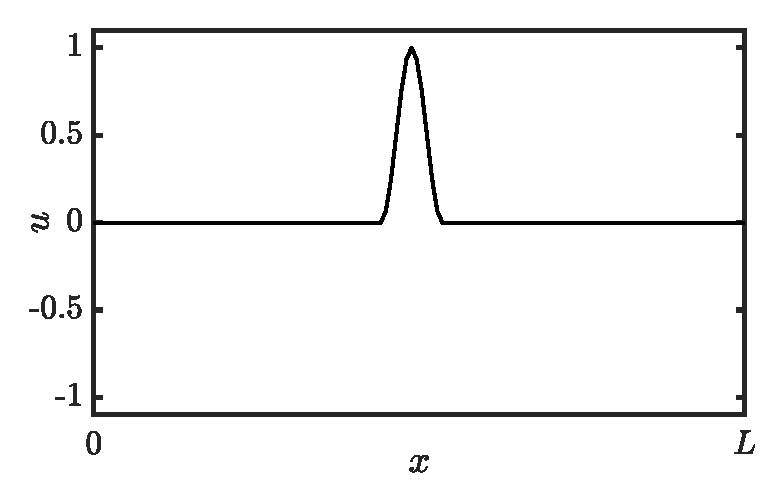
\includegraphics[width=\figWidth\textwidth]{figures/resonators/dispersion1.eps}}\hfill
    \subfloat[$t = 1$ ms.\label{fig:dispersion2}]{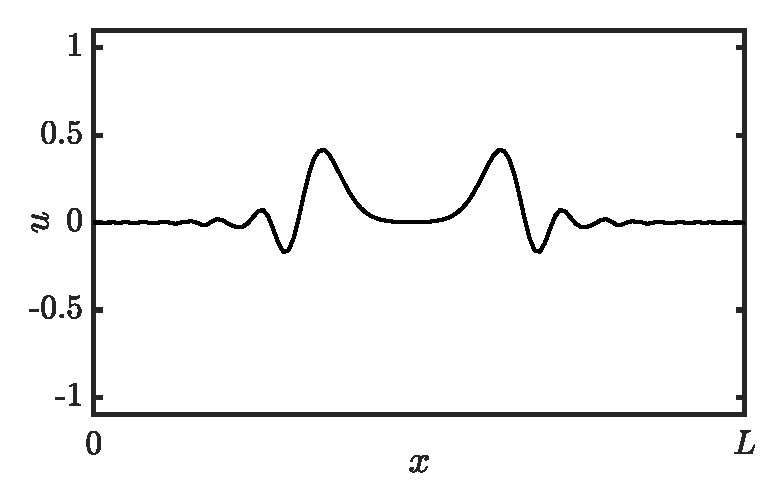
\includegraphics[width=\figWidth\textwidth]{figures/resonators/dispersion2.eps}}\hfill
    \subfloat[$t = 2$ ms.\label{fig:dispersion3}]{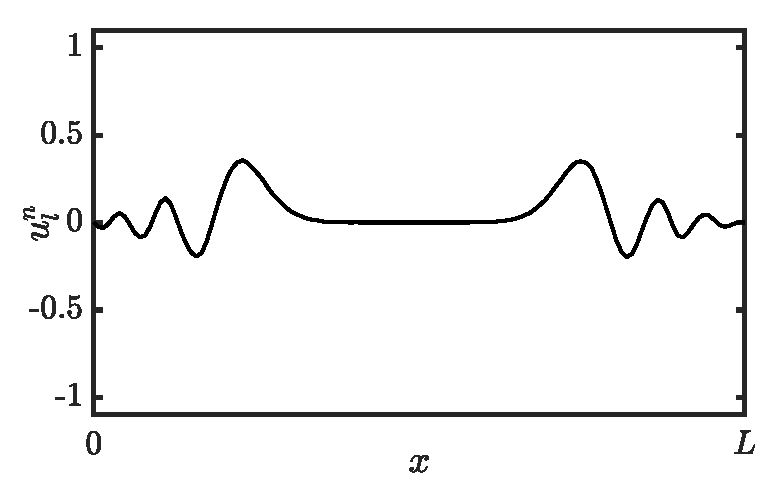
\includegraphics[width=\figWidth\textwidth]{figures/resonators/dispersion3.eps}}
    \caption{Frequency dispersion in a stiff string due to stiffness.\label{fig:dispersion}}
\end{figure}

% \subsubsection{Dispersion Analysis \SWcomment[or: Frequency Dispersion]}
% The 4\thOrder spatial derivative models \textit{frequency dispersion}, a phenomenon that causes different frequencies to travel at different speeds. As opposed to the undesired numerical dispersion 

% \SWcomment[not done]

\subsection{Adding losses}
Before moving on to the discretisation of the PDE in Eq. \eqref{eq:stiffStringPDENoLosses}, losses can be added to the system. In the physical world, strings lose energy through e.g. air viscosity and thermoelastic effects. All frequencies lose energy and die out (damp) over time, but higher frequencies do so at a much faster rate. This phenomenon is called \textit{frequency-dependent damping} and can be modelled using a mixed derivative $\pt \pxx$. This way of frequency-dependent damping first appeared in \cite{Bensa2003} and has been used extensively in the literature since (see e.g. \cite{Webb2015, Bilbao2019}). A damped stiff string can be modelled as
\begin{equation}\label{eq:stiffStringPDE}
    \rho A \ptt u = T \pxx u - EI \pxxxx u - 2 \sz \rho A \pt u + 2 \so \rho A\pt \pxx u,
\end{equation}
where the non-negative loss coefficients $\sz$ (in s$^{-1}$) and $\so$ (in m$^2$/s) determine the frequency-independent and frequency-dependent losses respectively. Appendix \ref{app:intuitionSigma1} attempts to provide some intuition on workings of these damping terms.

A more compact way to write Eq. \eqref{eq:stiffStringPDE}, %and is also found often in the literature (see e.g. \cite{theBible,Bilbao2009Modular})
is to divide all terms by $\rho A$ to get
\begin{equation}\label{eq:stiffStringPDECompact}
    \ptt u = c^2 \pxx u - \kappa^2 \pxxxx u - 2 \sz \pt u + 2 \so \pt \pxx u.
\end{equation} 

% \subsubsection{Intuition}
% Although Eq. \eqref{eq:stiffStringPDE} might look daunting at first, the principle of Newton's second law remains the same. 

% \SWcomment[Something about the 4th spatial derivative and the loss terms here...]

\subsubsection{Boundary conditions}
Section \ref{sec:1DWave} presents two types of boundary conditions for the 1D wave equation in Eq. \eqref{eq:boundaryCond1DWave}. In the case of the stiff string, these can be extended to
\begin{subequations}\label{eq:stiffStringBoundConds}
    \begin{align}
        u = \px u &= 0 \quad \text{(clamped)}\label{eq:BCclamped}\\
        u = \pxx u &= 0 \quad \text{(simply supported)}\label{eq:BCsimplySupported}\\
        \pxx u = \pxxx u &= 0 \quad \text{(free)}\label{eq:BCfree}
    \end{align}
\end{subequations}
at $x = 0, L$. See Figure \ref{fig:boundaryCondsStiffString} for plots of the first modal shape for each respective boundary condition.\footnote{Note that there is a zero-frequency mode if free boundary conditions are used for both ends of the string, which is technically the first mode.} If simply supported boundary conditions are chosen, and for low values of $\kappa$, the frequencies exhibited by the system can be expressed in terms of the fundamental frequency $f_0 = c/2L$ (as in Eq. \eqref{eq:fundamentalFreq}) and frequency of partial $p$ (in Hz) is defined as \cite{Fletcher1964}
\begin{equation}\label{eq:inharmonicityEquation}
    f_p = f_0 p \sqrt{1 + B p^2},
\end{equation}
with inharmonicity coefficient 
\begin{equation*}
    B = \frac{\kappa^2 \pi^2}{c^2}.
\end{equation*}
\def\figWidth{0.32}
\begin{figure}[h]
    \centering
    \subfloat[Clamped.\label{fig:clamped}]{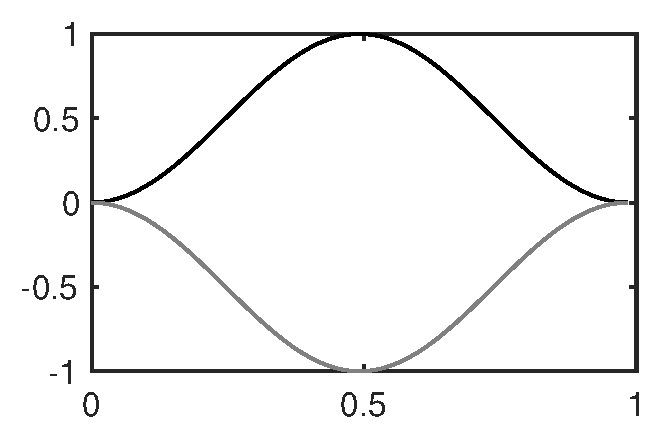
\includegraphics[width=\figWidth\textwidth]{figures/resonators/clamped.eps}}\hfill
    \subfloat[Simply supported.\label{fig:simplySupported}]{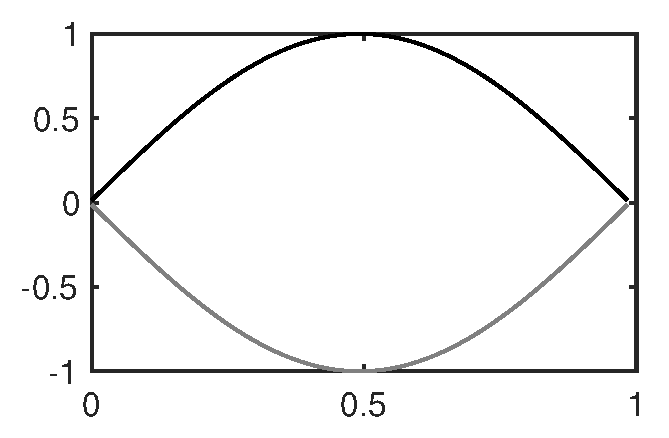
\includegraphics[width=\figWidth\textwidth]{figures/resonators/simplySupported.eps}}\hfill
    \subfloat[Free.\label{fig:free}]{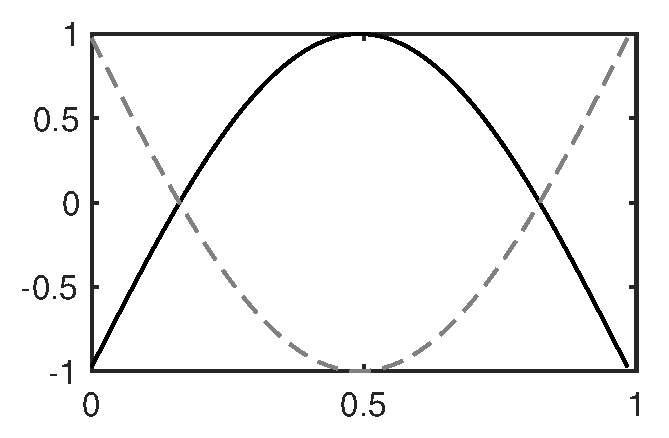
\includegraphics[width=\figWidth\textwidth]{figures/resonators/free.eps}}
    \caption{Plots of the first (normalised) modal shape for the three boundary conditions in Eqs. \eqref{eq:stiffStringBoundConds}. The extremes are indicated with solid black and dashed grey lines respectively. \label{fig:boundaryCondsStiffString}}
\end{figure}

\section{Discrete time}\label{sec:stiffStringDiscrete}
For the sake of compactness, Eq. \eqref{eq:stiffStringPDECompact} will be used in the following. Naturally, the same process can be followed for Eq. \eqref{eq:stiffStringPDE}, the only difference being a multiplication by $\rho A$ of all terms.

Following Section \ref{sec:gridFunctions} and using the FD operators presented in Section \ref{sec:FDoperators}, Eq. \eqref{eq:stiffStringPDECompact} can be discretised as 
\begin{equation}\label{eq:stiffStringFDS}
    \dtt \uln = c^2 \dxx \uln - \kappa^2 \dxxxx \uln - 2 \sz \dtd \uln + 2 \so\dtm\dxx \uln,
\end{equation}
and is defined for domain $l\in\{0, \hdots, N\}$ and number of grid points $N+1$. 
The $\dxxxx$ operator is defined as the second-order spatial difference in Eq. \eqref{eq:discSecondSpace} applied to itself:
\begin{equation}\label{eq:dxxxx}
    \dxxxx = \dxx\dxx = \frac{1}{h^4}\left(e_{x+}^2 - 4e_{x+}+6 - 4e_{x-}+e_{x-}^2\right).
\end{equation} 
A multiplication of two shift operators applied to a grid function simply means to apply each shift individually. 
% The $\dxxxx$ operator applied to $\uln$ thus becomes
% \begin{equation}
%     \dxxxx\uln = \frac{1}{h^4}\left(u_{l+2}^n - 4u_{l+1}^n+6\uln - 4u_{l-1}^n+u_{l-2}^n\right).
% \end{equation}

A definition for the mixed-derivative operator can similarly be found.
Recalling the definitions for $\dtm$ in Eq. \eqref{eq:backwardTimeOperator} and $\dxx$ Eq. \eqref{eq:discSecondSpace}, their combination results in
\begin{align}
    \dtm\dxx &= \frac{1}{k}\left(1-e_{t-}\right)\frac{1}{h^2}\left(e_{x+}-2+e_{x-}\right),\nonumber \\
    &= \frac{1}{kh^2}\left(e_{x+}-2+e_{x-} - e_{t-}(e_{x+}-2+e_{x-})\right).
\end{align}
To have two different shift operators multiplied together still simply means to apply each of them to the grid function individually. 
% The $\dtm\dxx$ operator applied to $\uln$ thus yields
% \begin{equation}
%     \dtm \dxx \uln = \frac{1}{hk^2}\left(u_{l+1}^n - 2 \uln + u_{l-1}^n - u_{l+1}^{n-1} + 2 u_l^{n-1} - u_{l-1}^{n-1}\right).
% \end{equation}
The reason a backwards difference is used here is to keep the system \textit{explicit}. A scheme is explicit if the values of $u_l^{n+1}$ can be calculated from known values at times $n$ and $n-1$. If this is not the case and values of e.g. $u_{l+1}^{n+1}$ and $u_{l-1}^{n+1}$ are required to calculate $u_l^{n+1}$, the scheme is called \textit{implicit}. An example of an implicit scheme, that uses the centred operator for the temporal derivative in the frequency-dependent damping term instead, can be found in Section \ref{sec:implicitStiffString}.

Using the definitions above, 
the operators in scheme \eqref{eq:stiffStringFDS} can be expanded, and after a multiplication of all terms by $k^2$ and collecting the terms, this yields
% \begin{equation}
%     \begin{aligned}\label{eq:expandedStringFDS}
%         \frac{1}{k^2}\big(u_l^{n+1} - 2\uln & + u_l^{n-1} \big) =\frac{c^2}{h^2}\left(u_{l+1}^n - 2\uln + u_{l-1}^n\right) \\
%         &- \frac{\kappa^2}{h^4}\left(u_{l+2}^n - 4u_{l+1}^n+6\uln - 4u_{l-1}^n+u_{l-2}^n\right) \\ 
%         &- \frac{\sz}{k} \left(u_l^{n+1} - u_l^{n-1}\right)\\
%         & + \frac{2\so}{kh^2}\left(u_{l+1}^n - 2\uln + u_{l-1}^n - u_{l+1}^{n-1} + 2u_l^{n-1} + u_{l-1}^{n-1}\right),
%     \end{aligned}
% \end{equation}
% and after multiplication by $k^2$ and collecting the terms yields
\begin{equation}\label{eq:stiffStringUpdate}
    \begin{aligned}
        (1+\sz k) u_l^{n+1} =&\ \left(2 - 2\lambda^2 - 6\mu^2 - \frac{4\so k}{h^2}\right) \uln\\
        & + \left(\lambda^2 + 4\mu^2 + \frac{2\so k}{h^2}\right) (u_{l+1}^n + u_{l-1}^n) \\
        &- \mu^2 (u_{l+2}^n + u_{l-2}^n) + \left(-1+\sz k + \frac{4\so k}{h^2}\right)u_l^{n-1}\\
        & - \frac{2\so k}{h^2}(u_{l+1}^{n-1} + u_{l-1}^{n-1}),
    \end{aligned}
\end{equation}
with 
\begin{equation}\label{eq:stiffStringCourant}
    \lambda = \frac{ck}{h} \qaq \mu = \frac{\kappa k}{h^2}.
\end{equation}
The update equation follows by dividing both sides by $(1+\sz k)$. 

The stability condition for the FD scheme in \eqref{eq:stiffStringFDS} is defined as 
\begin{equation}\label{eq:stiffStringStability}
    h \geq \sqrt{\frac{c^2k^2+4\so k + \sqrt{(c^2k^2 + 4\so k)^2+16\kappa^2k^2}}{2}},
\end{equation}
and will be derived in Section \ref{sec:stiffStringStability} using von Neumann analysis. 
This condition can then be used to calculate the number of intervals $N$ in a similar fashion as for the 1D wave equation shown in Eq. \eqref{eq:orderOfCalc}. First, Eq. \eqref{eq:stiffStringStability} should be satisfied with equality, after which the following calculations are performed:
\begin{equation*}
    N := \floor[\frac{L}{h}] \qaq h := \frac{L}{N},
\end{equation*}
which can then be used to calculate $\lambda$ and $\mu$ in Eq. \eqref{eq:stiffStringCourant}.

\subsubsection{Stencil}
As done in Section \ref{sec:1DWaveDisc}, a stencil for the FD scheme in Eq. 
\eqref{eq:stiffStringFDS} can be created, and is shown in Figure \ref{fig:stencilStiffString}. In order to calculate $u_l^{n+1}$, $5$ points at the current time step are needed due to the 4\thOrder spatial derivative. Due to the mixed derivative in the frequency-dependent damping term, neighbouring points at the previous time step are also required. 
%, the coefficient multiplied onto $u_l^{n+1}$.

% and the terms collected to obtain the following update equation
% \begin{equation}
%     \begin{aligned}
%     % (1+\sz k) u_l^{n+1} =&\ \left(2 - 2\lambda^2 - 6\mu^2 - \frac{4\so k}{h^2}\right) \uln\\
%     % & + \left(\lambda^2 + 4\mu^2 + \frac{2\so k}{h^2}\right) (u_{l+1}^n + u_{l-1}^n) \\
%     % &- \mu^2 (u_{l+2}^n + u_{l-2}^n) + \left(-1+\sz k + \frac{4\sz k}{h^2}\right)u_l^{n-1}\\
%     % & - \frac{2\so k}{h^2}(u_{l+1}^{n-1} + u_{l-1}^{n-1})
%     % \end{aligned}
%     Au_l^{n+1} = &\ B_0 \uln + B_1 (u_{l+1}^n + u_{l-1}^n) + B_2 (u_{l+2}^n + u_{l-2}^n) \\
%     &+ C_0 u_l^{n-1} + C_1(u_{l+1}^{n-1} + u_{l-1}^{n-1}) 
%     \end{aligned}
% \end{equation}
% with coefficients
% \begin{gather*}
%     B_0 = 2 - 2\lambda^2 - 6\mu^2 - \frac{4\so k}{h^2}, \quad B_1 = \lambda^2 + 4\mu^2 + \frac{2\so k}{h^2}, \quad B_2 =- \mu^2, \\[1em]
%     C_0 =  -1+\sz k + \frac{4\so k}{h^2},\quad C_1 = - \frac{2\so k}{h^2}, \qaq A = 1+\sz k.
% \end{gather*}
% Note that for clarity the division by $A$ has been left for implementation. 
\begin{figure}[h]
    \centering
    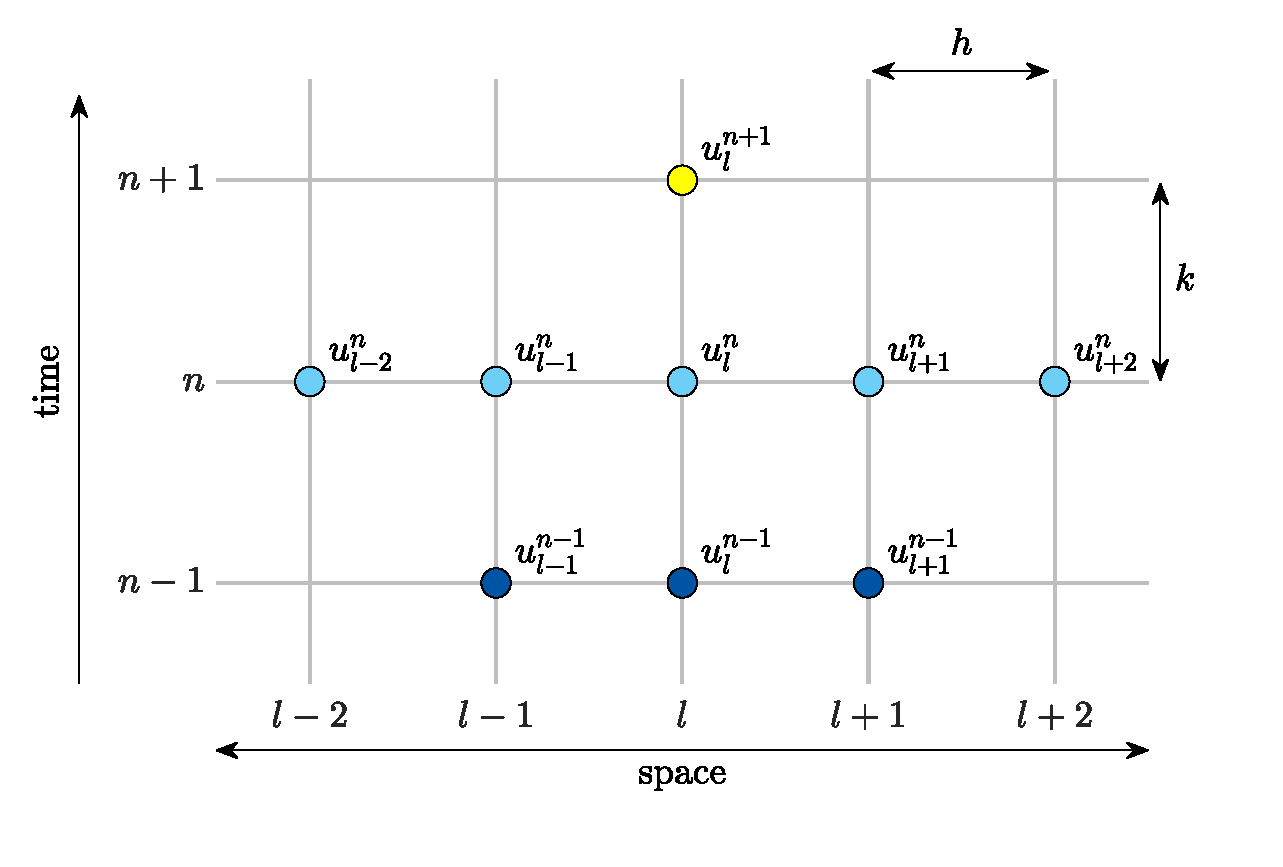
\includegraphics[width=0.8\textwidth]{figures/resonators/stencilDampedStiffString.eps}
    \caption{The stencil for the damped stiff string scheme in Eq. \eqref{eq:stiffStringFDS} (adapted from \citeP[A]).\label{fig:stencilStiffString}}
\end{figure}

\subsection{Boundary conditions}\label{sec:stiffStringBoundaryConditions}
Due to the 4\thOrder spatial derivative, two virtual grid points need to be accounted for at the boundaries of the system. Discretising the boundary conditions in \eqref{eq:stiffStringBoundConds} yields
\begin{subequations}\label{eq:stiffStringBoundCondsDisc}
    \begin{align}
        \uln = \delta_{x\pm} \uln &= 0 \quad \text{(clamped)}\label{eq:BCclampedDisc}\\
        \uln = \dxx \uln &= 0 \quad \text{(simply supported)}\label{eq:BCsimplySupportedDisc}\\
        \dxx \uln = \dxd\dxx \uln &= 0 \quad \text{(free)}\label{eq:BCfreeDisc}
    \end{align}
\end{subequations}
at $l = 0, N$. The operator in the clamped condition uses the $\dxp$ operator at the left boundary ($l = 0$) and $\dxm$ at the right ($l = N$). Notice that to discretise $\px^3$ in the free boundary condition in Eq. \eqref{eq:BCfree}, the more accurate $\dxd\dxx$ operator has been chosen over the less accurate $\dxm \dxx$ and $\dxp \dxx$ operators for the left and right boundary respectively.

Below, the boundary conditions are expanded to obtain definitions for the virtual grid points. 

\subsubsection{Clamped}
Expanding the operators for the clamped condition yields 
\begin{equation}
    u_0^n = u_1^n = 0 \qaq u_{N-1}^n = u_N^n = 0.
\end{equation}
This can be simplified by reducing the range of calculation to $l\in \{ 2, \hdots, N-2\}$.

\subsubsection{Simply supported}
As the states of the end points of a system with simply supported boundary conditions are $0$ at all times, the range of calculation can be reduced to $l\in \{ 1, \hdots, N-1\}$. Evaluating the update equation in Eq. \eqref{eq:stiffStringUpdate} at $l=1$ and $l=N-1$ shows that definitions for the virtual grid points $u_{-1}^n$ and $u_{N+1}^n$ are required. A definition for $u_{-1}^n$ can be found by expanding Eq. \eqref{eq:BCsimplySupportedDisc} at $l = 0$:
\begin{align}
    &\frac{1}{h^2}\left(u_1^n - 2 u_0^n + u_{-1}^n\right) = 0,\nonumber\\[-1em]
    \xLeftrightarrow{\mystrut\ u^n_0 = 0\ } \quad & u_1^n + u_{-1}^n = 0,\nonumber\\[0.25em]
    &u_{-1}^n = -u_1^n,\label{eq:simplySupportedResult}
\end{align}
and similarly for $u_{N+1}^n$ by expanding the condition at $l=N$:
\begin{equation*}
    u_{N+1}^n = -u_{N-1}^n.
\end{equation*}
Substituting the first definition into the expanded scheme in Eq. \eqref{eq:stiffStringUpdate} at $l=1$, yields
\begin{equation}
    \begin{aligned}
        \!\!\!(1+\sz k) u_1^{n+1} =&\ \left(2 - 2\lambda^2 - 5\mu^2 - \frac{4\so k}{h^2}\right) u_1^n + \left(\lambda^2 + 4\mu^2 + \frac{2\so k}{h^2}\right) u_{2}^n \!\!\\
        &-\mu^2u_3^n+ \left(-1+\sz k + \frac{4\sz k}{h^2}\right)u_1^{n-1} - \frac{2\so k}{h^2}u_{2}^{n-1}.
    \end{aligned}
\end{equation}
Doing the same for $l=N-1$ yields
\begin{equation}
    \begin{aligned}
        \!\!(1+\sz k) u_{N-1}^{n+1} =&\ \left(2 - 2\lambda^2 - 5\mu^2 - \frac{4\so k}{h^2}\right) u_{N-1}^n + \left(\lambda^2 + 4\mu^2 + \frac{2\so k}{h^2}\right) u_{N-2}^n \\
        &-\mu^2u_{N-3}^n+ \left(-1+\sz k + \frac{4\sz k}{h^2}\right)u_{N-1}^{n-1} - \frac{2\so k}{h^2}u_{N-2}^{n-1}.
    \end{aligned}
\end{equation}

\subsubsection{Free}
Although rarely used for the stiff string (rather for the ideal bar), free boundary conditions are given here for completeness. The free boundary condition requires all points to be calculated and the range of calculation remains $l\in\{0, \hdots, N\}$. At each respective boundary, two virtual grid points are needed: $u_{-1}^n$ and $u_{-2}^n$ at the left and $u_{N+1}^n$ and $u_{N+2}^n$ at the right boundary respectively.
The third-order spatial FD operator in Eq. \eqref{eq:BCfreeDisc} is defined as:
\begin{align}
    \dxd\dxx &= \frac{1}{2h^3}\left(e_{x+}-e_{x-}\right)\left(e_{x+}-2+e_{x-}\right),\nonumber\\
    &=\frac{1}{2h^3}\left(e_{x+}^2 - 2e_{x+} + 2e_{x-} -e_{x-}^2\right),
\end{align}
and can be used to solve for $u_{-2}^n$ at $l=0$:
\begin{align*}
    \frac{1}{2h^3} &\left(u_2^n - 2 u_1^n + 2u_{-1}^n - u_{-2}^n\right) = 0,\\%[0.25em]
    u_{-2}^n &= u_2^n - 2 u_1^n + 2u_{-1}^n.
    % \\[-1em]
    % \!\!\!\!\!\!\!\!\!\!\!\!\!\!\!\xLeftrightarrow{\mystrut\ \dxx \uln = 0\ \Rightarrow\ \text{ Eq. \eqref{eq:simplySupportedResult}}\ }
    % \quad u_{-2}^n &= u_2^n - 4 u_1^n 
\end{align*}
As $u_0^n$ is not necessarily $0$ at all times, solving the first part of the boundary condition (i.e., $\dxx u_0^n = 0$) yields a different result than in the simply supported case:
\begin{align*}
   &\frac{1}{h^2} \left(u_1^n - 2 u_0^n + u_{-1}^n \right) = 0,\\
    &u_{-1}^n = 2u_0^n - u_1^n.
    % \\[-1em]
    % \!\!\!\!\!\!\!\!\!\!\!\!\!\!\!\xLeftrightarrow{\mystrut\ \dxx \uln = 0\ \Rightarrow\ \text{ Eq. \eqref{eq:simplySupportedResult}}\ }
    % \quad u_{-2}^n &= u_2^n - 4 u_1^n 
\end{align*}
The same can be done at $l=N$ to get the following definitions for the virtual grid points
\begin{equation*}
    u_{N+2}^n = u_{N-2}^n - 2 u_{N-1}^n + 2u_{N+1}^n
    \qaq u_{N+1}^n = 2u_N^n - u_{N-1}^n.
\end{equation*}
The update equations for the boundary points will not be given here. Instead the matrix form of the FD scheme with free boundaries will be provided below. 
% The update equation at $l=0$ then becomes
% \begin{equation}
%     \begin{aligned}
%         \!\!\!\!\!(1+\sz k) u_0^{n+1} =&\ \left(2 - 2\lambda^2 - 2 \mu^2 - \frac{4\so k}{h^2}\right) u_0^n + \left(\lambda^2 +4\mu^2 + \frac{4\so k}{h^2}\right) u_1^n \\
%         &-2\mu^2u_2^n+ \left(-1+\sz k + \frac{4\sz k}{h^2}\right)u_0^{n-1} - \frac{4\so k}{h^2}u_1^{n-1}.
%     \end{aligned}
% \end{equation}
% at $l=1$
% \begin{equation}
%     \begin{aligned}
%         \!\!\!\!\!(1+\sz k) u_1^{n+1} =&\ \left(2 - 2\lambda^2 - 5\mu^2 - \frac{4\so k}{h^2}\right) u_1^n + \left(\lambda^2 + 4\mu^2 + \frac{2\so k}{h^2}\right) u_{2}^n \\
%         &-2\mu^2u_3^n+ \left(-1+\sz k + \frac{4\sz k}{h^2}\right)u_1^{n-1} - \frac{2\so k}{h^2}u_{2}^{n-1}.
%     \end{aligned}
% \end{equation}
\subsubsection{Discussion}
In practice, the simply supported boundary condition is mostly chosen as this most realistically reflects string terminations in the real world. The clamped condition could be chosen for simplicity as this does not require an alternative update at the boundaries. The free boundary condition is more often used to model the boundaries of (damped) ideal bar (Eq. \eqref{eq:stiffStringPDE} with $T = 0$).

\subsection{Implementation and matrix form}\label{sec:implementationStiffString}
When using \texttt{MATLAB}, for a more compact implementation, it is useful to write the scheme in matrix form (see Section \ref{sec:matrixForm}). The FD scheme of the stiff string in \eqref{eq:stiffStringFDS} can be written as 
\begin{equation}\label{eq:matrixFormStiffString}
    A\u^{n+1} = \B\u^n + \C \u^{n-1}
\end{equation}
where 
\begin{equation*}
    \begin{gathered}
    A = (1+\sz k), \quad \B = 2\I + c^2 k^2 \Dxx - \kappa^2 k^2 \Dxxxx + 2 \so k \Dxx, \\
    \text{and} \quad \C = -(1-\sz k)\I - 2\so k \Dxx.
    \end{gathered}
\end{equation*}
Notice that $A$ is a scalar rather than a matrix.

The size of the state vectors and the matrix-form operators depend on the boundary conditions. For clamped conditions, the state vectors ($\u^{n+1}$, $\u^n$ and $\u^{n-1}$) and matrices will be of size $(N-3) \times 1$ and $(N-3) \times (N-3)$ respectively. The $\Dxx$ matrix will be of the form given in Eq. \eqref{eq:DxxDef} and the matrix form of the $\dxxxx$ operator is
\begin{equation}
    \mathbf{D}_{xxxx} = \frac{1}{h^4}\begin{bmatrix}
        6& -4 & 1 & & \mathbf{0} \\
        -4 & 6 &\ddots &\ddots & \\
        1& \ddots & \ddots & \ddots&1 \\
        &\ddots & \ddots & 6 & -4 \\
        \mathbf{0} & & 1& -4 & 6 \\
    \end{bmatrix}.
\end{equation}

For simply supported conditions, the state vectors and matrices will be of size $(N-1) \times 1$ and $(N-1) \times (N-1)$ respectively. Again, $\Dxx$ is as defined in Eq. \eqref{eq:DxxDef} and $\Dxxxx$ can be obtained by multiplying two $\Dxx$ matrices according to 
\begin{equation}
    \mathbf{D}_{xxxx} = \Dxx\Dxx = \frac{1}{h^4}\begin{bmatrix}
        5& -4 & 1 & & & \mathbf{0}& \\
        -4 & 6 &\ddots &\ddots & & & \\
        1& \ddots & \ddots & -4 & 1 & & \\
        & \ddots& -4 & 6 & -4 & \ddots& \\
        & & 1 & -4 & \ddots & \ddots &1 \\
        & & & \ddots & \ddots & 6 & -4 \\
        & \mathbf{0} & & & 1& -4 & 5 \\
    \end{bmatrix}.
\end{equation}

Finally for free boundary conditions given in Eq. \eqref{eq:BCfreeDisc}, the state vectors and matrices are $(N+1)\times 1$ and $(N+1)\times (N+1)$ respectively. Now, the $\Dxx$ matrix is of the form in Eq. \eqref{eq:DxxDefNeumann} instead, and

\setstackgap{L}{16pt}
\setstacktabbedgap{8pt}
\def\lrgap{\kern3pt}
\fixTABwidth{T}
\begin{equation}
    \mathbf{D}_{xxxx} = \frac{1}{h^4}\xbracketMatrixstack{
        2& -4 & 2 & & & \mathbf{0}& \\
        -2 & 5 & -4 & 1 & & & \\
        1& -4 & 6 & -4 & 1 & & \\
        & \ddots & \ddots & \ddots & \ddots &\ddots & \\
        & & 1 & -4 & 6 & -4 &1 \\
        & & & 1 & -4 & 5 & -2 \\
        & \mathbf{0} & & & 2& -4 & 2}.
\end{equation}

\subsection{Parameters and output}\label{sec:paramsAndOutput}
The values of the parameters naturally determine the properties of the output sound. Where in the 1D wave equation, only the fundamental frequency $f_0$ could be affected (through $c$ and $L$ in Eq. \eqref{eq:fundamentalFreq}), the stiff string has many more aspects that can be changed. See Table \ref{tab:stiffStringParams} for parameters most commonly used in this project. 
\begin{table}[h]
    \begin{center}
    \begin{tabular}{|l|c|c|}
        \hline
        Name & Symbol (unit) & Value\\ \hline
        Length & $L$ (m) & $1$\\
        Material density & $\rho$ (kg/m$^3$) & $7850$\\
        Radius & $r$ (m) & $5\cdot10^{-4}$\\
        Tension & $T$ (N) &$100 \leq T \leq 10^4$\\
        Young's modulus & $E$ (Pa) & $2\cdot10^{11}$\\
        Freq.-independent damping & $\sz$ (s$^{-1}$) & $1$\\
        Freq.-dependent damping & $\so$ (m$^2$/s) & $0.005$\\\hline
    \end{tabular}
    \caption{Parameters and their values most commonly used over the course of this project.\label{tab:stiffStringParams}}
    \end{center}
\end{table}
{\renewcommand{\arraystretch}{1}

A formula exists to calculate the loss coefficients $\sz$ and $\so$ from $T_{60}$ values at different frequencies (see \cite[Eq. (7.29)]{theBible}). During this project, however, these values have been tuned by ear and are usually set to be approximately those found in Table \ref{tab:stiffStringParams}. 


\subsubsection{Output}
Figure \ref{fig:stiffStringOutput} shows the time domain and frequency domain output (retrieved at $l = \floor[N/20]$) of an implementation of the stiff string excited using a raised-cosine (see Chapter \ref{ch:physInspExcitations}). The parameters used can be found in Table \ref{tab:stiffStringParams} 
where $T = 3951$ N, and $r = 9.35\cdot 10^{-4}$ m to highlight dispersive effects. Finally, simply supported boundary conditions are chosen. From the left panel, one can observe that over time, dispersive effects show, where higher-frequency components in the excitation travel faster through the medium than lower-frequency components. In frequency domain (the right panel in Figure \ref{fig:stiffStringOutput}), this shows in the fact that the partials are not perfect integer multiples of the fundamental. Notice that the partials are closer to each other for lower frequencies and further apart as their frequency increases. Finally, the frequency-dependent damping term causes higher frequencies to have a lower amplitude than lower frequencies. 

Apart from the obvious material properties such as density, stiffness and geometry, perceptual qualities of the sound are surprisingly much determined by $\so$, and for lower values the output can become extremely metallic.

\begin{figure}[h]
    \centering
    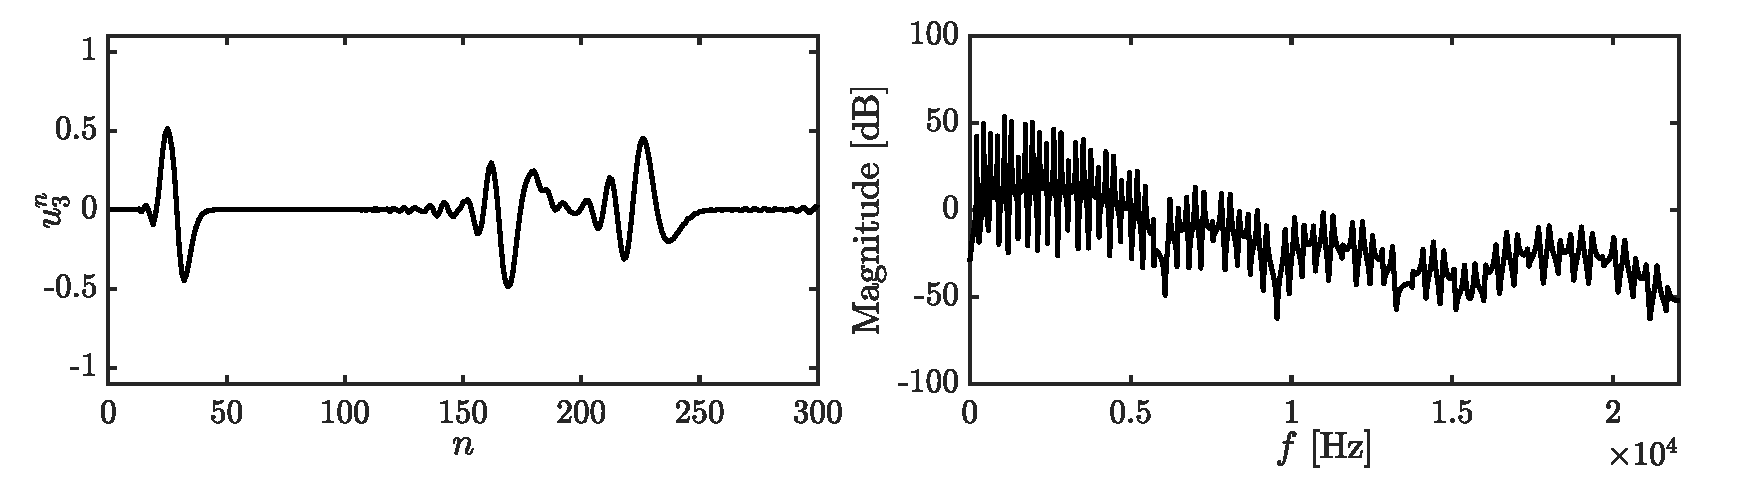
\includegraphics[width=\textwidth]{figures/resonators/outputFFT.eps}
    \caption{The time-domain and frequency domain output of the stiff string. The parameters are set as in Table \ref{tab:stiffStringParams} where $r = 9.35\cdot 10^{-4}$ m to highlight dispersive effects and $T = 3951$ N. %From the left panel, one can observe that over time, dispersive effects show due to the stiffness in the string. In frequency domain (right panel) this shows through the partials not being perfect integer multiples of the fundamental. Lastly, higher frequency components have a lower amplitude due to the frequency-dependent damping.
    \label{fig:stiffStringOutput}}
\end{figure}


\section{von Neumann analysis and stability condition}\label{sec:stiffStringStability}
In order to obtain the stability condition for the damped stiff string, one can perform a von Neumann analysis, as presented in Section \ref{sec:stabilityAnalysis}, on the FD scheme in Eq. \eqref{eq:stiffStringFDS}. A detailed derivation can be found in Appendix \ref{app:vonNeumannString}, and a compact version will be presented here.

Using the definitions found in Eq. \eqref{eq:temporalAnsatz} for the temporal operators, and Eqs. \eqref{eq:dxxAnsatz} and \eqref{eq:dxxxxAnsatz} for the spatial operators, the frequency domain representation of Eq. \eqref{eq:stiffStringFDS} can be obtained:
\begin{align*}
    \!\!\!\!\frac{1}{k^2}\left(z - 2 + z^{-1}\right) =&-\frac{4c^2}{h^2}\sin^2(\beta h/2) - \frac{16\kappa^2}{h^4}\sin^4(\beta h/2) - \frac{\sz}{k}z + \frac{\sz}{k}z^{-1}\\
    & - \frac{8 \so}{kh^2}\sin^2(\beta h/2) + \frac{8 \so}{kh^2} \sin^2(\beta h/2)z^{-1},
\end{align*}
and after collecting the terms, the characteristic equation is as follows
\begin{gather}
    (1+\sz k)z + \left(16\mu^2\sin^4(\beta h/2)+\left(4\lambda^2+\frac{8\so k}{h^2}\right)\sin^2(\beta h/2) - 2\right)\nonumber\\
    +\left(1-\sz k-\frac{8\so k}{h^2}\sin^2(\beta h/2)\right)z^{-1}=0.\label{eq:charDampedString}
\end{gather}
Rewriting this to the form in Eq. \eqref{eq:polynomialForm}, and using condition \eqref{eq:condition214}, its roots can be shown to be bounded by unity for all $\beta$ under the following condition (see Appendix \ref{app:vonNeumannString})
\begin{align*}
    4\mu^2+\lambda^2+ \frac{4\so k}{h^2}&\leq 1.
\end{align*}
Recalling the definitions for $\lambda$ and $\mu$ from Eq. \eqref{eq:stiffStringCourant}, one yields a quadratic equation in $h^2$ which can be shown to be bounded by
\begin{equation}
    h \geq \sqrt{\frac{c^2k^2+4\so k + \sqrt{(c^2k^2 + 4\so k)^2+16\kappa^2k^2}}{2}}.
\end{equation}
This is the stability condition for the damped stiff string also shown in Eq. \eqref{eq:stiffStringStability}.

\section{Energy analysis}\label{sec:energyAnalysisString}
As mentioned in Section \ref{sec:energyAnalysis}, it is useful to perform the energy analysis on the scheme with all physical parameters written out. Discretising the PDE in Eq. \eqref{eq:stiffStringPDE} yields
\begin{equation}
    \rho A \dtt \uln = T \dxx \uln - EI \dxxxx \uln - 2\sz \rho A \dtd \uln + 2 \so \rho A \dtm \dxx \uln,
\end{equation}
defined for $l\in d$ with discrete domain $d = \{0, \hdots, N\}$. This section will follow the 4 steps described in Section \ref{sec:energyAnalysis}.

\subsubsection{Step 1: Obtain $\dtp \h$}
The first step is to take the inner product (see Eq. \eqref{eq:discInnerProd}) of the scheme with $(\dtd \uln)$ over discrete domain $d$:
\begin{equation}\label{eq:rOCStiffString}
    \begin{aligned}
    \dtp \h =&\ \rho A \langle \dtd \uln, \dtt \uln \rangle_d - T \langle \dtd \uln, \dxx \uln\rangle_d + EI \langle \dtd \uln, \dxxxx \uln \rangle_d\\
    & + 2\sz\rho A \langle \dtd \uln, \dtd \uln \rangle_d - 2\so \rho A\langle \dtd \uln, \dtm \dxx \uln \rangle_d = 0.
    \end{aligned}
\end{equation}  
% If the free boundary conditions in \eqref{eq:BCfreeDisc} are used, the primed inner product in Eq. \eqref{eq:primedInnerProd} needs to be used. Here we continue with clamped / simply supported boundaries.

\subsubsection{Step 2: Identify energy types and isolate $\dtp$}
As there is damping present in the system, and the system is distributed, the energy balance will be of the form 
\begin{equation}
    \dtp \h = \mathfrak{b}-\mathfrak{q},
\end{equation}
with boundary term $\b$ and damping term $\q$. The latter is defined as
\begin{equation}\label{eq:dampingTermStiffString}
    \mathfrak{q} = 2\sz \rho A \lVert\dtd\uln\rVert_d^2 - 2 \so \rho A \langle \dtd \uln, \dtm \dxx \uln \rangle_d,
\end{equation}
where the virtual grid points needed to calculate the second term are defined by the boundary conditions given in Eq. \eqref{eq:stiffStringBoundCondsDisc}. Furthermore, $\mathfrak{b}$ appears after rewriting Eq. \eqref{eq:rOCStiffString} using summation by parts (see Section \ref{sec:summationByParts}), specifically, using Eq. \eqref{eq:summationByPartsMinusBar} for the second term and Eq. \eqref{eq:summationByPartsTwiceReduced} for the third, yields
\begin{align*}
    \dtp \h &= \rho A \langle \dtd \uln, \dtt \uln \rangle_d + T \langle \dtd \dxp \uln, \dxp \uln\rangle_{\underline{d}} + EI \langle \dtd \dxx \uln, \dxx \uln \rangle_{\overline{\underline{d}}} \\
    &= \mathfrak{b} - \mathfrak{q},
\end{align*}
where the boundary term becomes
\begin{align*}
    \mathfrak{b} =&\ T\Big((\dtd u_N^n)(\dxp u_N^n) - (\dtd u_0^n) (\dxp u_{-1}^n)\Big) \\
    &+ EI \Big((\dtd u_N^n)(\dxp \dxx u_N^n) - (\dxx u_N^n)(\dxm \dtd u_N^n) \Big)\\
    &- EI \Big((\dtd u_0^n)(\dxm \dxx u_0^n) - (\dxx u_0^n)(\dxp \dtd u_0^n)\Big).
\end{align*}
For the clamped and simply supported boundary conditions in \eqref{eq:BCclampedDisc} and \eqref{eq:BCsimplySupportedDisc} it can easily be shown that $\mathfrak{b} = 0$. If free conditions as in Eq. \eqref{eq:BCfreeDisc} are used, the boundary conditions will vanish when the primed inner product in Eq. \eqref{eq:primedInnerProd} is used in Step 1 and identity \eqref{eq:summationByPartsTwicePrimed} is used when performing summation by parts. Below, only the simply supported case will be considered. 

Isolating $\dtp$ to obtain the total energy $\h$ in the definition for $\dtp \h$ above, requires identities \eqref{eq:prodIdentity1} and \eqref{eq:prodIdentity2} and yields
\begin{equation*}
    \begin{aligned}
        \dtp\h &= \dtp\left(\frac{\rho A}{2}\lVert\dtm \uln\rVert_d^2 + \frac{T}{2}\langle\dxp\uln, e_{t-}\dxp\uln\rangle_{\underline{d}} + \frac{EI}{2}\langle\dxx\uln, e_{t-}\dxx\uln\rangle_{\overline{\underline{d}}}\right) \\
        &=-\mathfrak{q}.
    \end{aligned}
\end{equation*}
From this, the definition for the Hamiltonian $\h$, the kinetic energy $\t$ and potential energy $\v$ can be found:
\begin{equation}\label{eq:energyBalanceStiffString}
    \begin{gathered}
        \h = \t + \v, \qwiq \t = \frac{\rho A}{2}\lVert\dtm \uln\rVert^2_d,\quad \text{and} \\
        \v = \frac{T}{2}\langle\dxp\uln, e_{t-}\dxp\uln\rangle_{\underline{d}} + \frac{EI}{2}\langle\dxx\uln, e_{t-}\dxx\uln\rangle_{\overline{\underline{d}}}\ ,
    \end{gathered}
\end{equation}
and can be shown to be non-negative if condition \eqref{eq:stiffStringStability} is satisfied.

\subsubsection{Step 3: Check units}
Comparing the acquired definitions in Eq. \eqref{eq:energyBalanceStiffString} to those for the 1D wave equation in Eq. \eqref{eq:energyBalance1DWave}, one can observe that the definitions are nearly identical, the only difference being the second term in the definition for $\v$ in Eq. \eqref{eq:energyBalanceStiffString}. 
Writing this term out in units, and recalling that Pa (the unit for $E$) in SI units is kg$\cdot$m$^{-1}\cdot$s$^{-2}$, yields
\begin{align*}
    \frac{EI}{2}\langle\dxx\uln, e_{t-}\dxx\uln\rangle_{\overline{\underline{d}}}\ \overset{\text{in units}}{\xrightarrow{\hspace*{1cm}}}& \quad \text{Pa}\cdot \text{m}^4 \cdot \text{m} \cdot (\text{m}^{-2} \cdot \text{m} \cdot \text{m}^{-2} \cdot \text{m}) \\
    & = \text{kg} \cdot \text{m}^2 \cdot \text{s}^{-2},
\end{align*}
and indeed has the correct units. 

As described in Section \ref{sec:energyAnalysis}, the damping terms in $\mathfrak{q}$ need to have units of Joules per second, or kg $\cdot$ m$^2 \cdot$ s$^{-3}$. Writing the terms in Eq. \eqref{eq:dampingTermStiffString} out in their units yields
\begin{align*}
    2\sz \rho A \lVert\dtd\uln\rVert_d^2\ \overset{\text{in units}}{\xrightarrow{\hspace*{1cm}}}&\quad \text{s}^{-1}\cdot\text{kg}\cdot\text{m}^{-3}\cdot\text{m}^2\cdot \text{m}\cdot(\text{s}^{-1}\cdot\text{m})^2 \\
    &= \text{kg} \cdot \text{m}^2 \cdot \text{s}^{-3},\\
    - 2 \so \rho A \langle \dtd \uln, \dtm \dxx \uln \rangle_d\  \overset{\text{in units}}{\xrightarrow{\hspace*{1cm}}}&\quad \text{m}^2\cdot\text{s}^{-1}\cdot\text{kg}\cdot\text{m}^{-3}\cdot\text{m}^2\\
    &\qquad\cdot\text{m}\cdot(\text{s}^{-1}\cdot\text{m})(\text{s}^{-1}\cdot\text{m}^{-2}\cdot \text{m})\\
    &= \text{kg} \cdot \text{m}^2 \cdot \text{s}^{-3},
\end{align*}
which also have the correct units.
\subsubsection{Step 4: Implementation}
An implementation of the energy calculation for the simply supported boundary condition is given in Algorithm \ref{alg:stiffStringEnergy}. The calculation of the damping is omitted, but the full algorithm (including other boundary conditions) can be found online \cite{stringGist}. Figure \ref{fig:energyStiffString} shows that the damping present in the system causes $\h$ to decrease in the left panel. The right panel shows that the deviation of the total energy calculated using Eq. \eqref{eq:normalisedEnergyDamping} is within machine precision.
\\
\noindent
\begin{minipage}{\textwidth}
\setlstMAT
\begin{lstlisting}[caption=Calculating $\h$ for the simply supported boundary condition., label=alg:stiffStringEnergy]
%%%% Before the main loop: %%%%

% Initialise Dx+ operator to calculate potential energy due to tension
% As the domain is reduced by one, the matrix needs to be of size N x N
Dxp = sparse(1:N, 1:N, -ones(1, N), N, N) + ...
sparse(1:N-1, 2:N, ones(1, N-1), N, N);

%%%% In the main loop: %%%%

% energy in the system
kinEnergy(n) = rho * A * h / 2 * sum((1/k * (u - uPrev)).^2);
potEnergy(n) = T / 2 * h * sum((Dxp * [0; u]) .* (Dxp * [0; uPrev])) ... + E * I * h / 2 * sum((Dxx * u) .* (Dxx * uPrev));
\end{lstlisting}
\end{minipage}

\begin{figure}[h]
    \centering
    \begin{tikzpicture}[->,node distance=3cm,
        thick,main node/.style={circle,draw}]
    
        \node[] (image) at (0,0) {
        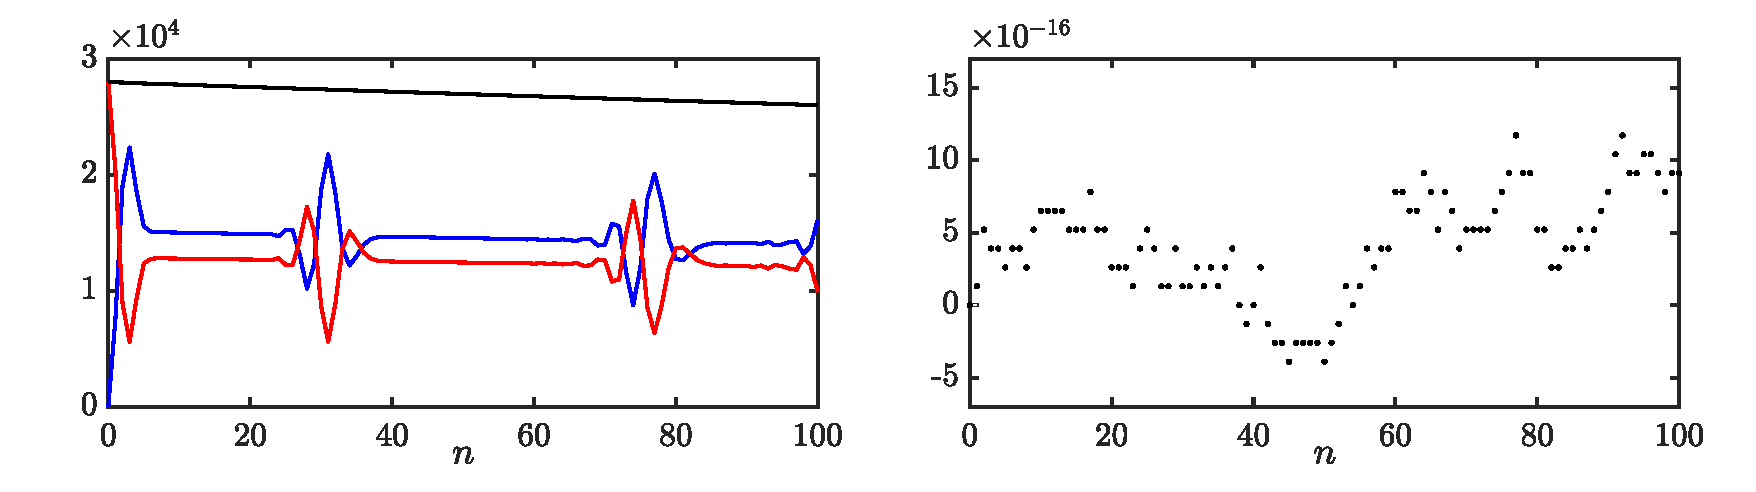
\includegraphics[width=\textwidth]{figures/resonators/stiffStringEnergy.eps}
        };
    
        \node[] (he) at (0.2,0.5) {\small $\mathfrak{h}_\text{e}$};

        \node[] (h) at (-5.75, 1) {\small $\mathfrak{h}$};
        \node[] (v) at (-5.75, 0.5) {\small $\color{red}\mathfrak{v}$};
        \node[] (t) at (-5.75, 0) {\small $\color{blue}\mathfrak{t}$};
      \end{tikzpicture}
      \caption{The kinetic (blue), potential (red), and total (black) energy of an implementation of the stiff string are plotted in the left panel. The right panel shows the normalised energy (according to Eq. \eqref{eq:normalisedEnergyDamping}) and shows that the deviation of the energy is within machine precision. \label{fig:energyStiffString}}
\end{figure}

\section{Modal analysis}\label{sec:stiffStringModalAnalysis}
% To find an expression for the modal frequencies one can ignore the damping terms for now and follow the process in Section \ref{sec:modalAnalysis} to obtain
% \begin{equation}
%     f_p = \frac{1}{\pi k}\sin^{-1}\left(\frac{1}{2}\sqrt{-\eig_p(c^2k^2\Dxx - \kappa^2k^2\Dxxxx)}\right).
% \end{equation}

To be able to perform a modal analysis on the FD scheme in Eq. \eqref{eq:stiffStringFDS}, it must be written in a one-step form -- introduced in Section \ref{sec:oneStepForm} -- due to the damping present in the system. Using the matrix form of the damped stiff string in Eq. \eqref{eq:matrixFormStiffString}, the one-step form can be written as
%needs be used. As there are damping terms present in the system, it is useful to write the update in one-step form as explained in Section \ref{sec:oneStepForm}.
\begin{equation}\label{eq:oneStepFormStiffSTring}
    \underbrace{\begin{bmatrix}
        \u^{n+1}\\
        \u^n
    \end{bmatrix}}_{\w^{n+1}} = 
    \underbrace{\begin{bmatrix}
        \B/A & \C/A\\
        \I & \mathbf{0}
    \end{bmatrix}}_{\Q}
    \underbrace{\begin{bmatrix}
        \u^n\\
        \u^{n-1}
    \end{bmatrix}}_{\w^n},
\end{equation}
where the definitions for $\B$, $\C$ and $A$ can be found in Section \ref{sec:implementationStiffString}. In this analysis, the definitions for $\Dxx$ and $\Dxxxx$ for simply supported boundary conditions will be used.

Assuming test solutions of the form $\w^n = z^n\boldPhi$, and recalling that $z=e^{sk}$ and complex frequency $s = j\omega + \sigma$ (see Section \ref{sec:oneStepForm}), yields the following eigenvalue problem (see Section \ref{sec:eigenValueProblems}):
\begin{equation}
    z\boldPhi = \Q \boldPhi,
\end{equation}
which can be solved for the $p$\th complex modal frequency
\begin{equation}
    s_p = \frac{1}{k}\ln \left(\eig_p(\Q)\right).
\end{equation}
The (angular) frequency of the $p$\th mode can then be obtained using $\mathfrak{I}(s_p)$ and the damping per mode as $\mathfrak{R}(s_p)$. Only selecting the non-negative frequencies obtained from $\mathfrak{I}(s_p)$, these can be plotted, and are shown in Figure \ref{fig:modesStiffString}. The parameters used are the ones found in Table \ref{tab:stiffStringParams} with $T = 1.88\cdot 10^6$ N, and $r = 1.58\cdot 10^{-2}$ m, which are unnaturally high values to highlight inharmonic behaviour. The left panel shows that the system is indeed inharmonic, i.e., modal frequencies increase more as the modal number increases. The right panel shows that higher modes exhibit a higher amount of damping. This is due to the frequency-dependent damping term. If $\sigma_1 = 0$ in Eq. \eqref{eq:stiffStringFDS}, it can be shown that $\sigma_p = \sigma_0$ for every mode $p$ (in this case $\sigma_0 = -1$).

\begin{figure}[t]
    \centering
    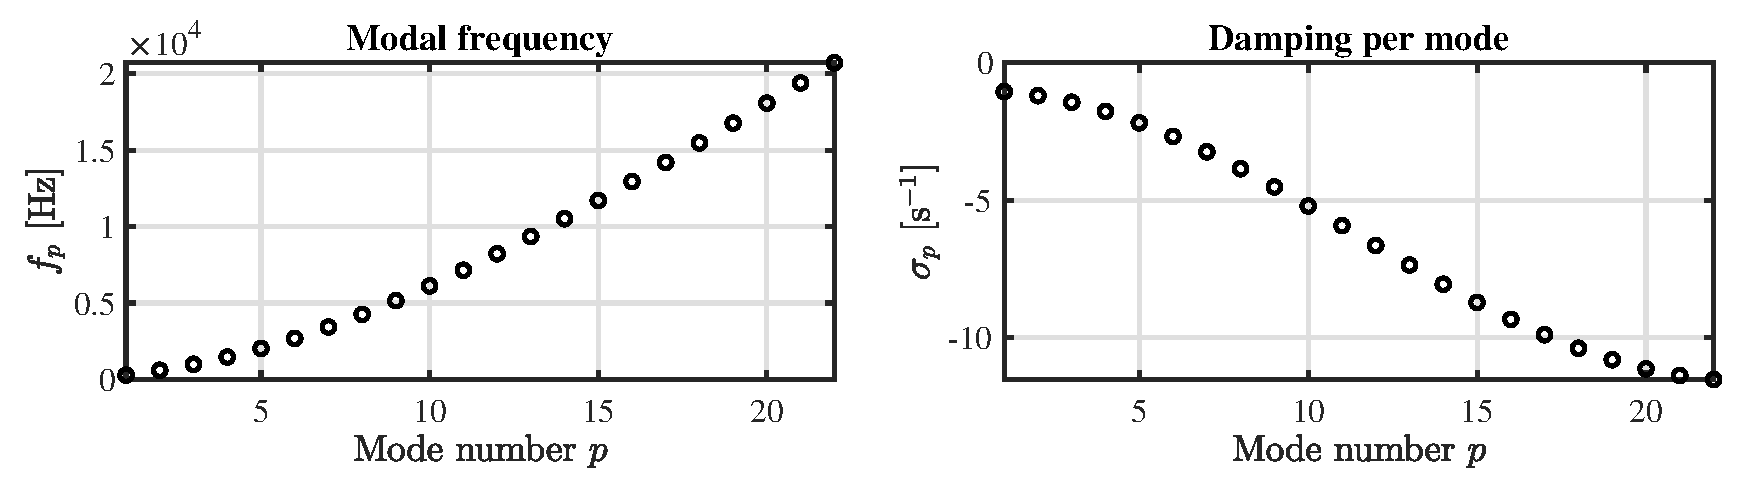
\includegraphics[width=\textwidth]{figures/resonators/modesStiffString.eps}
    \caption{The modal frequencies and damping per mode for the stiff string using the values in Table \ref{tab:stiffStringParams} and $T = 1.88\cdot 10^6$ N and $r = 1.58\cdot 10^{-2}$ m to highlight effects of stiffness. % Notice form the left panel that the frequency increases exponentially with the mode number. The right panel shows that higher modes exhibit a greater amount of damping due to the frequency-dependent damping term.
    \label{fig:modesStiffString}}
\end{figure}

\section{Implicit scheme}\label{sec:implicitStiffString}
Although not used in the published work of this project, it is useful to touch upon an example of an implicit scheme. Consider a discretisation of Eq. \eqref{eq:stiffStringPDECompact} where the (more accurate) centred operator is used for the frequency-dependent damping term:
\begin{equation}\label{eq:stiffStringFDSImplicit}
    \dtt \uln = c^2 \dxx \uln - \kappa^2 \dxxxx \uln - 2 \sz \dtd \uln + 2 \so\dtd\dxx \uln.
\end{equation}
Using the centred operator in the mixed-spatio-temporal operator renders the system \textit{implicit}, meaning that a definition for $u_l^{n+1}$ can not explicitly be found from known values. The stencil in Figure \ref{fig:stencilStiffStringImplicit} also shows this: in order to calculate $u_l^{n+1}$, neighbouring points at the next time step $u_{l+1}^{n+1}$ and $u_{l-1}^{n+1}$ are needed. The issue is that these values are unknown at the time of calculation.

Luckily, as the scheme is linear, it can be treated as a system of linear equations and solved following the technique described in Section \ref{sec:linearEquations}. The drawback is that this requires one matrix inversion per iteration which can be extremely costly.\footnote{In the context of FDTD methods, the matrices to be inverted are \textit{diagonally dominant}, which means that if the off-diagonals are small, specialised methods such as the iterative Jacobi method (see e.g. \cite{Saad2003}) could, with a few iterations, yield an answer for the inverse.} However, both von Neumann and modal analysis (below) show that using the centred instead of the backwards operator has a positive effect on the stability and the modal behaviour of the scheme. 

Considering simply supported boundary conditions such that the region of operation is $l \in \{1, \hdots, N-1\}$, the system will have $N-1$ unknowns ($u_l^{n+1}$ for $l \in \{1, \hdots, N-1\}$) that can be calculated using $N-1$ (update) equations. Writing this in matrix form using column vector $\u^n = [u_1^n, u_2^n, \hdots, u_{N-1}^n]$ yields 

\begin{equation}\label{eq:matrixFormStiffStringImplicit}
    \A\u^{n+1} = \B\u^n + \C \u^{n-1},
\end{equation}
where 
\begin{equation*}
    \begin{gathered}
    \A = (1+\sz k)\I - \so k\Dxx, \quad \B = c^2 k^2 \Dxx - \kappa^2 k^2 \Dxxxx, \\
    \text{and} \quad \C = -(1-\sz k)\I - \so k \Dxx.
    \end{gathered}
\end{equation*}
Equation \eqref{eq:matrixFormStiffStringImplicit} can be considered a system of linear equations (see Section \ref{sec:linearEquations}) and the state at the next time step $\u^{n+1}$ can then be retrieved using a matrix inversion (see \ref{sec:inverse})
\begin{equation}
    \u^{n+1} = \A^{-1}\left(\B\u^n + \C \u^{n-1}\right).
\end{equation}
\begin{figure}[h]
    \centering
    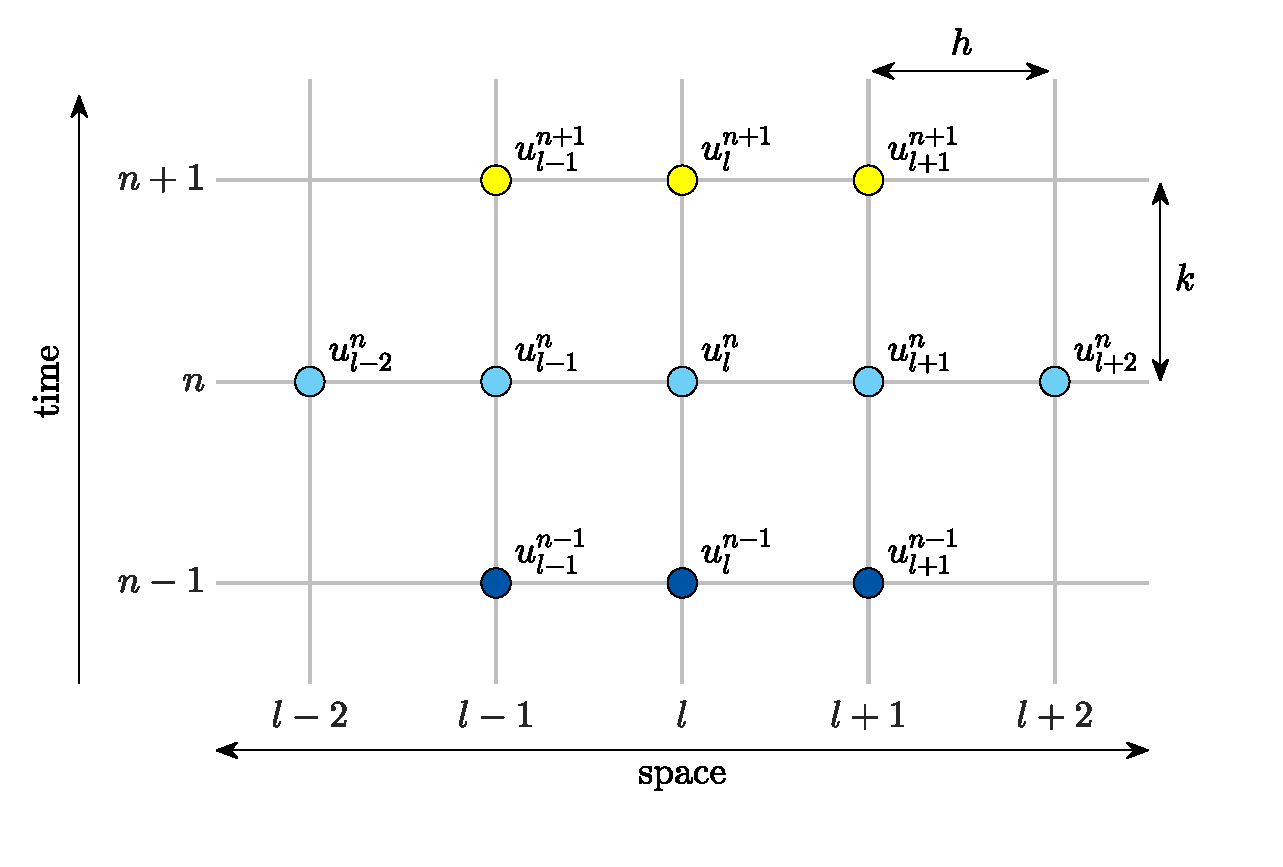
\includegraphics[width=0.8\textwidth]{figures/resonators/stencilImplicitStiffString.eps}
    \caption{The stencil for the damped stiff string scheme in \eqref{eq:stiffStringFDSImplicit}.\label{fig:stencilStiffStringImplicit}}
\end{figure}

\subsection{von Neumann analysis}\label{sec:stiffStringStabilityImplicit}
This section follows the same process as in Section \ref{sec:stiffStringStability}. A full derivation is given in Appendix \ref{app:vonNeumannStringImplicit} and a compact version is given here. 

The definitions in Section \ref{sec:stabilityAnalysis} can be used to obtain a frequency domain representation of the FD scheme in Eq. \eqref{eq:stiffStringFDSImplicit}:
\begin{align*}
    \!\!\!\!\frac{1}{k^2}\left(z - 2 + z^{-1}\right) =&-\frac{4c^2}{h^2}\sin^2(\beta h/2) - \frac{16\kappa^2}{h^4}\sin^4(\beta h/2) - \frac{\sz}{k}z + \frac{\sz}{k} z^{-1}\nonumber\\
    & - \frac{4 \so}{kh^2}\sin^2(\beta h/2)z + \frac{4 \so}{kh^2} \sin^2(\beta h/2)z^{-1},
\end{align*}
and collecting the terms, yields the following characteristic equation:
\begin{gather}
\left(1+\sz k + \frac{4\so k}{h^2}\sin^2(\beta h/2)\right)z + \left(16\mu^2\sin^4(\beta h/2)+4\lambda^2\sin^2(\beta h/2) - 2\right)\nonumber\\
+ \left(1-\sz k - \frac{4\so k}{h^2}\sin^2(\beta h/2)\right)z^{-1} = 0.\label{eq:charDampedImplicitStiffString}
\end{gather}
Rewriting this to the form found in Eq. \eqref{eq:polynomialForm} and using condition \eqref{eq:condition214}, one can show that its roots are bounded by unit for all $\beta$ under the following condition (see Appendix \ref{app:vonNeumannStringImplicit}):
\begin{equation*}
    4\mu^2+\lambda^2 \leq 1,
\end{equation*} 
and places the following condition on the grid spacing:
\begin{equation}\label{eq:implicitStability}
    h \geq \sqrt{\frac{c^2k^2 + \sqrt{c^4k^4 + 16\kappa^2k^2}}{2}}.
\end{equation}

Comparing this to the stability condition for the explicit scheme in Eq. \eqref{eq:stiffStringStability}, one can observe that the terms containing $\so$ have vanished. It can thus be concluded that, if the centred (rather than the backwards) difference is used to discretise the temporal derivative in the frequency-dependent damping term, $\so$ no longer influences the stability of the scheme and the condition is more relaxed. What this means in terms of behaviour of the scheme will be elaborated on in the following section.

\subsection{Modal analysis}
As the matrix form of the implicit FD scheme in Eq. \eqref{eq:matrixFormStiffStringImplicit} matches the form in Eq. \eqref{eq:modalForm}, one can perform a modal analysis by writing the scheme in a one-step form as explained in Section \ref{sec:oneStepForm}. The results of the analysis are shown in Figure \ref{fig:implicitModes} using the same values for $T$ and $r$ as in Section \ref{sec:stiffStringModalAnalysis}. To highlight the difference between using the backwards and centred difference for the frequency-dependent damping term, $\so$ has been set to $1$, which is much higher than one would normally use.

One can observe from Figure \ref{fig:implicitModes} that especially higher-frequency modes in the explicit scheme are affected by $\so$.  
In the continuous case, the modal frequencies should only be affected by values for $c$ and $\kappa$ as per Eq. \eqref{eq:inharmonicityEquation} and the damping should not influence the frequencies of the partials, as one could expect. However, as $\so$ increases, $h$ increases due to Eq. \eqref{eq:stiffStringStability}, causing $\lambda$ and $\mu$ to decrease. This introduces numerical dispersion as explained in Section \ref{sec:quality1DWave}, and the higher the value of $\so$, the more numerical dispersion is introduced.

As the stability condition for the implicit scheme in Eq. \eqref{eq:implicitStability} does not contain $\so$, this value will not affect $\lambda$ and $\mu$ and will thus not affect the modal frequencies. As can be observed from the figure, it even allows for one more grid point to be included in the simulation. It can be concluded that a more accurate simulation can be obtained with fewer numerically dispersive effects, because the frequency-dependent damping term no longer affects the stability condition for the implicit scheme.

\begin{figure}[h]
    \centering
    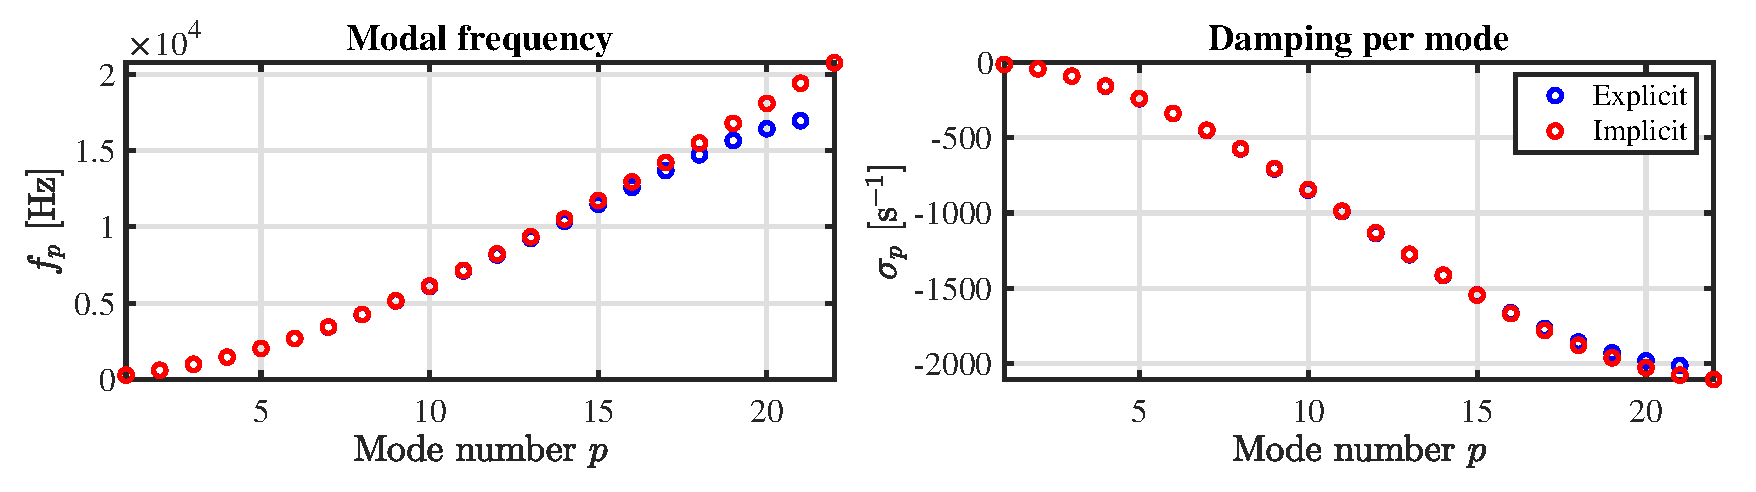
\includegraphics[width=\textwidth]{figures/resonators/implicitModes.eps}
    \caption{A comparison between the modal frequencies and damping per mode of the explicit (blue) and implicit (red) scheme. %Here, $T = 1885$ N, $E = 2\cdot10^{14}$ Pa and $\so = 1$ m$^2$/s to highlight differences between the two schemes. %One can observe that the modes of the implicit scheme follow the expected exponential pattern for the stiff string, where the explicit scheme shows numerically dispersive effects. Furthermore, due to the absence of $\so$ in the stability condition in Eq. \eqref{eq:implicitStability} and allows for one more grid point  
    \label{fig:implicitModes}}
\end{figure}

\subsection{Conclusion}
This section presented an implicit discretisation of the stiff string where the centred operator has been used to discretise the temporal derivative in the frequency-dependent damping term. By means of stability analysis and modal analysis, several advantages that the implicit scheme has over its explicit counterpart (presented in Section \ref{sec:stiffStringDiscrete}) have been shown.

As these advantages only show for higher values of $\so$, much higher than the ones used in this project, it has been chosen to use the explicit scheme for all further implementation. The decrease in accuracy is negligible for lower values of $\so$ and the calculation of the scheme becomes much more complex if the implicit scheme is used. 
\chapter{2D Systems}\label{ch:2Dsyst}


In this work, it is mainly used to model a simplified body in papers...


Rectangular system described by state variable $u = u(x,y,t)$  where $t\geq 0$ and $(x,y) \in \D$ where $\D$ is 2-dimensional. The state variable can then be discretised according to $u(x, y, t) \approx \ulmn$ with space $x = lh$ and $y = mh$ and time $t = nk$ and $k=1/\fs$. For simplicity the grid spacing in both the $x$ and $y$ directions are set to be the same but could be different.

Circular or elliptical systems can be modelled using a staircase approximation or radial coordinates \cite{theBible}

In continuous time the  operators:
\begin{equation}\label{eq:laplacian}
    \Delta = \pxx + \pyy
\end{equation}


The same shift operators as defined in Chapter \ref{ch:FDTD} can be applied to grid function $\ulmn$. Additional ones are
\begin{equation}
    e_{y+}\ulmn = u_{l, m+1}^n,\quad \text{and}\quad e_{y-}\ulmn= u_{l, m-1}^n.
\end{equation}

\section{Analysis Techniques in 2D}\label{sec:analysis2D}
Here, some of the differences between the analysis techniques presented in Chapter \ref{ch:analysis} and those in 2D will be elaborated on. Although, modal analysis remains the same

\subsection{Frequency Domain Analysis}
$p_x + p_y$

ansatz:
\begin{equation}
    \ulmn = z^n e^{jh(l\beta_x + m\beta_y)}
\end{equation}

\subsection{Energy Analysis}
Squared domain 
$d\in \{0, \hdots, N_x\} \times \{0, \hdots, N_y\}$
\begin{equation}\label{eq:2DInnerProd}
    \langle f^n, g^n \rangle_d = \sum_{l = 0}^{N_x}\sum_{m = 0}^{N_y} h^2 f_{l,m}^n g_{l,m}^n
\end{equation}

\subsection{Modal Analysis}
Stacked matrix form

\section{2D Wave Equation}
The 2D wave equation be used to model an ideal membrane such as done in 

It has identical behaviour to the 2D waveguide mesh presented by van Duyne and Smith \cite{Duyne1993}.

Consider a square ideal membrane with side lengths $L_x$ and $L_y$ (both in m) and its transverse displacement described by $u = u(x,y,t)$. The membrane is defined over $(x,y) \in \D$ with domain $\D = [0, L_x] \times[0, L_y]$ and its motion is described by the following PDE
\begin{equation}\label{eq:2DwavePDE}
    \ptt u = c^2\Delta u
\end{equation}
with wave speed $c = \sqrt{T/\rho H}$ (in m/s), tension per unit length (applied to the boundary)\todo{check whether this is right..}$T$ (in N/m), material density $\rho$ (in kg/m$^3$) and thickness $H$.

\section{Thin plate}
Used in \citeP[A], \citeP[B], \citeP[D] and \citeP[E]
biharmonic operator, Laplacian in \eqref{eq:laplacian} applied to itself.
\begin{equation}\label{eq:platePDE}
    \rho H \ptt u = -D\Delta\Delta u
\end{equation}
where $D = EH^3/12(1-\nu^2)$
\section{Stiff membrane}
Combination between Eqs. \eqref{eq:2DwavePDE} and \eqref{eq:platePDE}
\begin{equation}\label{eq:2DwavePDE}
    \rho H \ptt u = T\Delta u - D
    \Delta\Delta u
\end{equation}
\citeP[F]
\chapter{Acoustic Tubes}\label{ch:brass}

The dynamics of woodwind and brass instruments is based on wave propagation in acoustic tubes. Although the physical processes that generate the sound are fundamentally different from those in strings, the underlying models have many similarities. The main difference between acoustic tubes and the (ideal) strings, is that tubes have a varying cross-sectional area, causing wave dispersion and greatly influencing the modal frequencies and modal shapes present in the system.

In this work, planar wave propagation is assumed (rather than spherical), such that the behaviour of the systems can be approximated using 1D systems. Although higher-dimensional models might better capture some physical effects (see e.g. \cite{Kemp2002}), 1D systems already show good agreement between model and measurement \cite{Eveno2012}. Moreover, looking towards real-time implementation of these models, the choice to simplify to 1D has been made due to the low relative computational cost. 

This chapter first presents Webster's equation, which extends the 1D wave equation presented in Section \ref{sec:1DWave} by introducing a spatially varying cross-section. Although not used for the contributions in Part \ref{part:contributions}, Webster's equation forms a good basis for the second part of this chapter, which decomposes Webster's equation into a system of two coupled first-order PDEs. This has been used to model the trombone in paper \citeP[H].

\section{Webster's equation}\label{sec:webstersEq}
For an (axially symmetric) acoustic tube of length $L$ (in m) where the wavelengths of the frequencies at interest are much larger than the radius of the tube, one can simplify the system to be one-dimensional \cite{Bilbao2018}. For low-amplitude vibrations, the air propagation in this tube can be described using \textit{Webster}'s equation \cite{Webster1919}
\begin{equation}\label{eq:webstersPDE}
    S\partial_t^2\Psi = c^2\partial_x(S\partial_x\Psi),
\end{equation}
with \textit{acoustic potential} $\Psi = \Psi(x,t)$ (in m$^2$/s), the cross-sectional area along the tube, or bore profile $S = S(x)$ (in m$^2$) and the speed of sound in air $c$ (in m/s). The state variable $\Psi$ is defined for $t\geq 0$ and $x \in \D$ where domain $\D = [0, L]$. If $S(x)$ is constant, Eq. \eqref{eq:webstersPDE} reduces to the 1D wave equation in Eq. \eqref{eq:1DwavePDE}. This shows that for cylindrical acoustic tube, the fundamental frequency is not affected by the cross-sectional area, but solely relies on length $L$ and wave speed $c$ according to Eq. \eqref{eq:fundamentalFreq}. The acoustic potential can be related to pressure $p = p(x,t)$ (in Pa) and particle velocity $v = v(x,t)$ (in m/s) according to \cite{Bilbao2018}
\begin{equation}\label{eq:pressureVelocityWebster}
    p = \rho_0 \pt \Psi, \qaq v = -\px \Psi,
\end{equation}
with air density $\rho_0$ (in kg/m$^3$).

The interesting thing about the presence of a variable cross-section, is that it causes dispersive or scattering behaviour, especially at locations of high (spatial) variation of $S$. See Figure \ref{fig:websterPropagation}. Contrary to frequency dispersion as happens in a stiff string (see Chapter \ref{ch:stiffString}), all frequencies travel at the same speed, but some components of the wave get reflected due to the geometry of the tube.

\def\figWidth{0.32}
\begin{figure}[h]
    \centering
    \subfloat[$t = 1$ ms.\label{fig:websterPropagation1}]{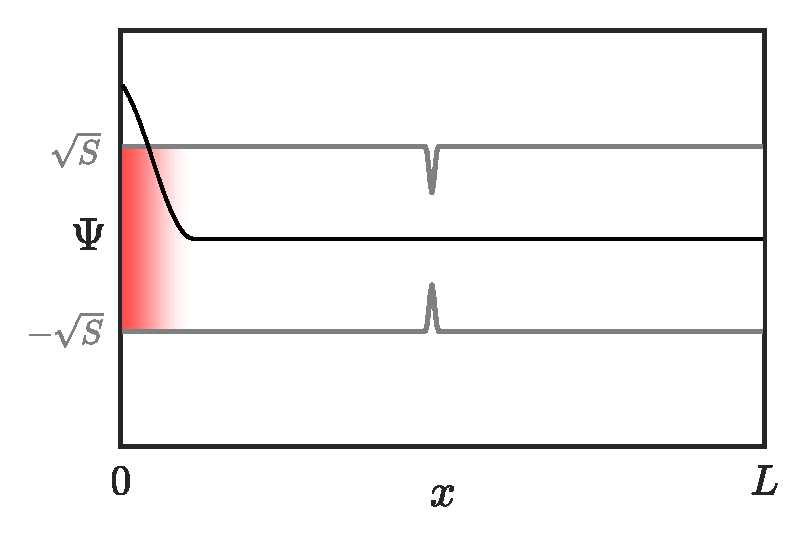
\includegraphics[width=\figWidth\textwidth]{figures/resonators/brass/websterPropagation1.eps}}\hfill
    \subfloat[$t = 5$ ms.\label{fig:websterPropagation2}]{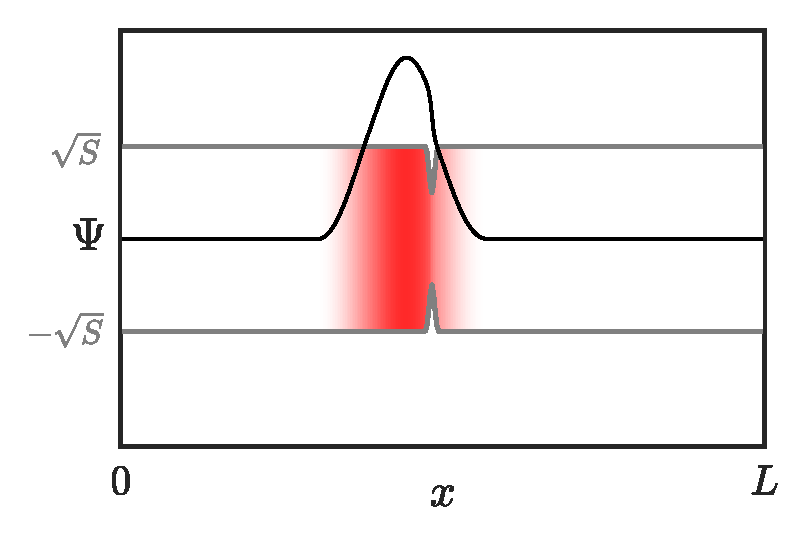
\includegraphics[width=\figWidth\textwidth]{figures/resonators/brass/websterPropagation2.eps}}\hfill
    \subfloat[$t = 8$ ms.\label{fig:websterPropagation3}]{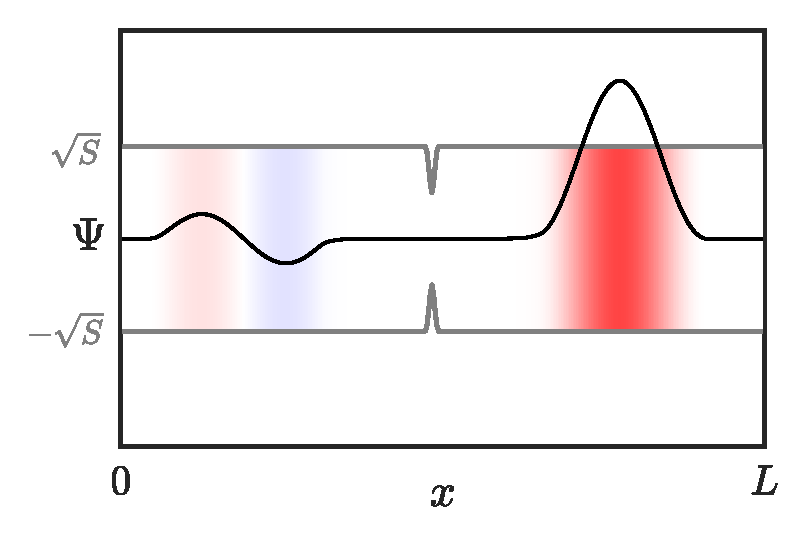
\includegraphics[width=\figWidth\textwidth]{figures/resonators/brass/websterPropagation3.eps}}
    \caption{Wave propagation and dispersion in an acoustic tube of varying cross-section (shown in grey) modelled by Webster's equation in Eq. \eqref{eq:webstersPDE}. Positive acoustic potential $\Psi$ is shown in red and negative in blue, which is also plotted for clarity. \label{fig:websterPropagation}}
\end{figure}
%test for git

\subsubsection{Boundary conditions}
The choices for boundary conditions in an acoustic tube are open and closed, defined as \cite{Bilbao2018}
\begin{subequations}\label{eq:contBoundariesBrass}
    \begin{align}
        \partial_t\Psi(0, t) &= 0, & \partial_t\Psi(L, t) &= 0, & &\text{(Dirichlet, open)},\label{eq:contDirichletBrass}\\
        \partial_x\Psi(0, t) &= 0, & \partial_x\Psi(L, t) &= 0, & &\text{(Neumann, closed)}\label{eq:contNeumannBrass}.
    \end{align}
\end{subequations}
This might be slightly counter-intuitive as when compared to the 1D wave equation, as ``closed" might imply the ``fixed" or Dirichlet boundary condition. The opposite can be intuitively shown by imagining a wave front with a positive acoustic potential (and thus positive pressure according to Eq. \eqref{eq:pressureVelocityWebster}) moving through a tube and hitting a closed end. What reflects is also a wave front with a positive acoustic potential, i.e., the sign of the potential does not flip. This also happens using the free or Neumann condition for the 1D wave equation (see Figure \ref{fig:boundaryCondsCont}).
Here, the following boundaries are chosen
\begin{equation}\label{eq:openClosed}
    \partial_x\Psi(0, t) = 0, \quad \text{and} \quad \partial_t\Psi(L, t) = 0,
\end{equation}
i.e. closed at the left end and open at the right end.

\subsection{Discrete time}
The state variable is discretised to the grid function $\Psi_l^n$ and is defined for $n\in \mathbb{N}^0$ and $l = \{0, \hdots, N\}$, where $N$ is the number of intervals between the grid points.
As the cross-section is distributed in space, $S(x)$ needs to be discretised to a grid function as well, albeit only in space (as it is not time-varying). Following \cite{Bilbao2018}, it is useful to introduce \textit{interleaved grid points} at $l-1/2$ and $l+1/2$ for $S$ and are defined as 
\begin{equation}\label{eq:sHalf}
    \Sm = \mxm S(x=lh), \qaq \Sp = \mxp S(x=lh),
\end{equation}
and approximate a `true' (possibly measured) bore profile $S(x)$ sampled at $x=lh$ with grid spacing $h$ (see Figure \ref{fig:variableCrossSection}). Using these definitions, one can discretise Eq. \eqref{eq:webstersPDE} to the following FD scheme \cite{theBible}\footnote{Notice that in \cite{theBible}, Webster's equation is $\Sbar_l \delta_{tt}\Psi^n_l = c^2\dxp(\Sm(\dxm\Psiln))$ but is identical to Eq. \eqref{eq:discWebster}. This discretisation has been chosen for a more straightforward energy analysis in Section \ref{sec:energyAnalysisWebster}.}
\begin{equation}\label{eq:discWebster}
    \Sbar_l \delta_{tt}\Psi^n_l = c^2\dxm\left(\Sp(\dxp\Psiln)\right),
\end{equation}
where
\begin{equation}\label{eq:Sbar}
    \Sbar_l = \mxp\Sm = \mxm\Sp = \mxx S(x=lh),
\end{equation}
the choice of which will become apparent in Section \ref{sec:stabilityEnergyWebster}.
The right-hand side of the scheme contains an operator applied to two grid functions ($S$ and $\Psi$) multiplied onto each other. In order to expand this, the product rule must be used. Recalling Eq. \eqref{eq:productRule} and applying this to backwards spatial operators instead yields
\begin{equation}
    \dxm (u_l^nw_l^n) = (\dxm u_l^n)(\mxm w_l^n) + (\mxm u_l^n)(\dxm w_l^n).
\end{equation}
Using the product rule, the right-hand side of Eq. \eqref{eq:discWebster} can be expanded to
\begin{equation*}
    \Sbar\dtt\Psiln = c^2\left[(\dxm \Sp)(\mxm (\dxp \Psiln)) + (\mxm \Sp)(\dxm (\dxp \Psiln))\right],
\end{equation*}
and solving for $\Psinp$ yields the following update equation (see Appendix \ref{app:webstersUpdateEq}):
\begin{equation}
    \Psinp = 2(1-\lambda^2)\Psiln-\Psinm+ \frac{\lambda^2\Sp}{\Sbar_l}\Psilp + \frac{\lambda^2\Sm}{\Sbar_l}\Psilm,\label{eq:webstersUpdateEq}
\end{equation}
with 
\begin{equation}
    \lambda = \frac{ck}{h},
\end{equation}
and similar to the 1D wave equation in Section \ref{sec:1DWaveDisc} needs to abide
\begin{equation}\label{eq:CFLwebster}
    \lambda \leq 1,
\end{equation}
in order for the scheme to be stable. See Section \ref{sec:stabilityEnergyWebster} for a derivation. The number of grid points $N$ can then be calculated in the same way as for the 1D wave equation in Eq. \eqref{eq:orderOfCalc}.

Notice that at the boundaries, Eq. \eqref{eq:webstersUpdateEq} requires values of $S$ (through its definition in Eq. \eqref{eq:Sbar}) outside of the defined domain, i.e., $S_{N+1/2}$ and $S_{-1/2}$. To solve this, one can set $\Sbar_0 = S(0)$ and $\Sbar_N = S(L)$ from which $S_{-1/2}$ and $S_{N+1/2}$ can be calculated according to
\begin{subequations}
    \begin{align}
        \Sbar_0 = \frac{1}{2}(S_{1/2} + S_{-1/2}) \ &\Rightarrow \ S_{-1/2} = 2\Sbar_0 - S_{1/2},\\
        \Sbar_N = \frac{1}{2}(S_{N+1/2} + S_{N-1/2}) \ &\Rightarrow \ S_{N+1/2} = 2\Sbar_N - S_{N-1/2}.\label{eq:Snph}
    \end{align} 
\end{subequations}
Although these values will not be needed when discretising the boundary conditions in Eq. \eqref{eq:contBoundariesBrass}, they will be useful at a later point.

\begin{figure}[t]
    \centering
    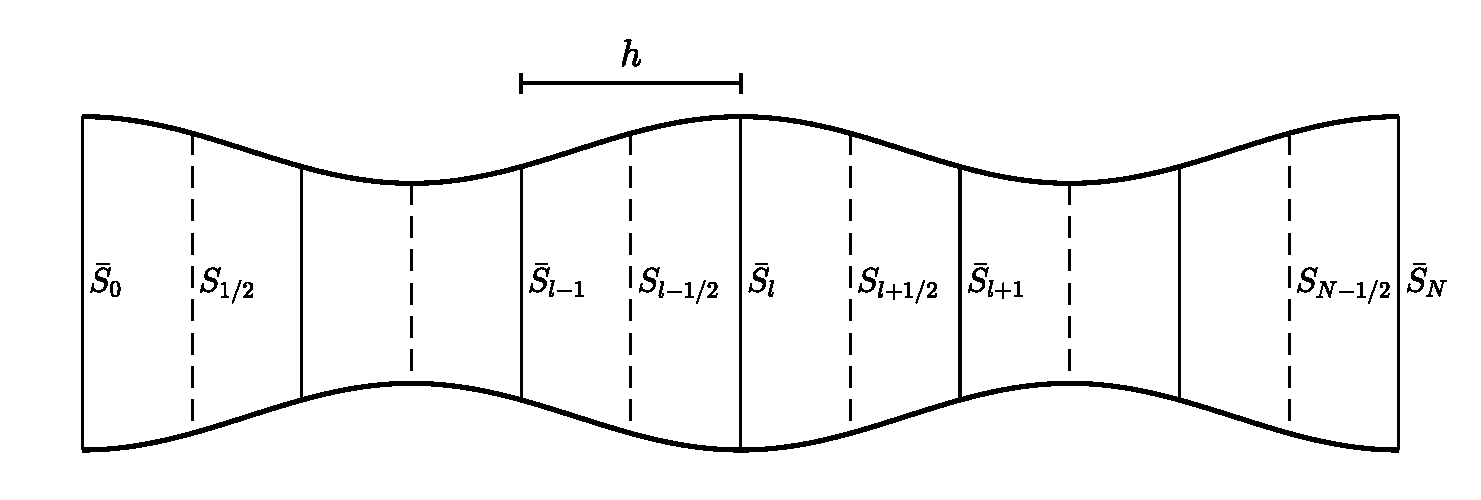
\includegraphics[width=0.9\textwidth]{figures/resonators/brass/variableCrossSection.eps}
    \caption{Approximations to $S(x)$ used in the FD scheme implementing Webster's equation. Dashed lines indicate the interleaved grid on which $S$ is sampled (Eq. \eqref{eq:sHalf}) and solid lines indicate $\Sbar$ which are averages of these (Eq. \eqref{eq:Sbar}). \label{fig:variableCrossSection}}
\end{figure}


\subsubsection{Boundary conditions}
One can discretise the continuous boundary conditions in Eq. \eqref{eq:openClosed} (closed at $x=0$, open at $x=L$) using centred difference operators for higher accuracy
\begin{subequations}\label{eq:discBoundariesBrass}
    \begin{align}
        \dxd\Psi_0^n &= 0 \quad \Rightarrow \quad\Psi_{-1}^n = \Psi_1^n ,\quad \!\!\!\!\!\!&&\text{(Neumann, closed)}, \label{eq:closedLeftBrass}\\
        \dtd\Psi_N^n &= 0\quad\Rightarrow \quad \Psi_N^n = 0, \quad \!\!\!\!\!\!&&\text{(Dirichlet, open)}\label{eq:openRightBrass}.
    \end{align}
\end{subequations} 
At the left boundary, Eq. \eqref{eq:webstersUpdateEq} can be expanded to:
\begin{equation*}
    \begin{aligned}
        \Psi_0^{n+1} &= 2(1-\lambda^2)\Psi_0^n-\Psi_0^{n-1}+ \frac{\lambda^2S_{1/2}}{\bar S_0}\Psi_1^n + \frac{\lambda^2S_{-1/2}}{\bar S_0}\Psi_{-1}^n,\\[-0.5em]
        \xLeftrightarrow{\mystrut\ \text{Eq. \eqref{eq:closedLeftBrass}}\ }\quad\Psi_0^{n+1} &= 2(1-\lambda^2)\Psi_0^n-\Psi_0^{n-1}+ \frac{\lambda^2(S_{1/2}+S_{-1/2})}{\bar S_0}\Psi_1^n,
    \end{aligned}
\end{equation*}
and as $\Sbar_0 = \frac{1}{2}(S_{1/2}+S_{-1/2})$ through Eq. \eqref{eq:Sbar}, this can be solved to
\begin{equation}\label{eq:leftBoundaryWebster}
    \Psi_0^{n+1} = 2(1-\lambda^2)\Psi_0^n-\Psi_0^{n-1}+ 2\lambda^2\Psi_1^n.
\end{equation}
One can implement the right boundary condition by simply reducing the range of operation to $l = \{0, \hdots, N-1\}$, as $\Psi_N^n = 0$ according to Eq. \eqref{eq:openRightBrass}. A more realistic boundary condition for the open end is presented in the following.

\subsection{Radiation}\label{sec:radiating}
One of the ways that an acoustic tube loses energy, is through radiation. The right boundary condition presented in Eq. \eqref{eq:openClosed} can be changed to be radiating according to \cite{theBible}
\begin{equation}\label{eq:radCont}
    \partial_x\Psi(L,t) = -a_1\partial_t\Psi(L,t)-a_2\Psi(L,t),
\end{equation}
where, for a tube terminating on an infinite plane \cite{Atig2004}
\begin{equation}
    a_1 = \frac{1}{2(0.8216)^2c}\ , \quad \text{and} \quad a_2 = \frac{L}{0.8216\sqrt{S_0S(1)/\pi}}\ ,
\end{equation}
which determine the amount of loss and inertia at the radiating boundary respectively. 

The radiating boundary in Eq. \eqref{eq:radCont} can then be discretised to \cite{theBible}
\begin{equation}\label{eq:centRadBound}
    \delta_{x\cdot}\Psi_N^n = -a_1\dtd\Psi_N^n - a_2\mu_{t\cdot}\Psi_N^n,
\end{equation}
which can be expanded and solved for $\Psi_{N+1}^n$ according to
\begin{equation}
    \Psi_{N+1}^n = h\left(-\frac{a_1}{k}(\Psi_N^{n+1} - \Psi_N^{n-1}) - a_2(\Psi_N^{n+1} + \Psi_N^{n-1})\right) + \Psi_{N-1}^n.
\end{equation}
Substitution into Eq. \eqref{eq:webstersUpdateEq} at the $l=N$ yields the following update equation
\begin{equation}
    \Psi_N^{n+1} = \frac{2(1-\lambda^2)\Psi_N^n-\Psi_N^{n-1}+\alpha_-\Psi_N^{n-1} + 2\lambda^2\Psi_{N-1}^n}{\left(1+\alpha_+\right)},
\end{equation}
where
\begin{equation}
    \alpha_\pm = h\left(\frac{a_1}{k}\pm a_2\right)\frac{\lambda^2S_{N+1/2}}{\bar S_N}.
\end{equation}
One can observe that $S_{N+1/2}$ is needed which is outside the defined domain. As mentioned before, setting $\Sbar_N = S(L)$, one can calculate $S_{N+1/2}$ using Eq. \eqref{eq:Snph} to solve the issue. 

\subsection{Excitation}\label{sec:webstersExcitation}
Although excitations will be discussed more in-depth in Part \ref{part:exciters}\todo{maybe refer to chapter/section instead}, a simple way to excite Webster's equation will be presented here.

Following \cite{Bilbao2018}, one can create an input signal $v_\text{in} = v_\text{in}(t)$ that interacts with the particle velocity of the tube. As this relates to the acoustic potential as in Eq. \eqref{eq:pressureVelocityWebster}, one can change the boundary condition of the left boundary to
\begin{equation}
    \px \Psi(0, t) = - v_\text{in}.
\end{equation}
Discretising this using the centred spatial operator yields
\begin{equation}
    \dxd \Psi_0^n = -v_\text{in}^n \quad \Rightarrow \quad \Psi_{-1}^n = 2h v_\text{in}^n + \Psi_1^n,
\end{equation}
and can be substituted into the update equation in Eq. \eqref{eq:webstersUpdateEq} at $l=0$ to get
\begin{align}
    \Psi_0^{n+1} &= 2(1-\lambda^2)\Psi_0^n-\Psi_0^{n-1} \frac{\lambda^2S_{1/2}}{\Sbar_0}\Psi_1^n + \frac{\lambda^2S_{-1/2}}{\Sbar_0}\left(2h v_\text{in}^n + \Psi_1^n\right),\nonumber\\
    \Psi_0^{n+1} &= 2(1-\lambda^2)\Psi_0^n-\Psi_0^{n-1} +2\lambda^2\Psi_1^n + \frac{2h\lambda^2S_{-1/2}}{\Sbar_0} v_\text{in}^n.
\end{align}
The input signal is arbitrary, but looking towards lip excitation, and following \cite{theBible}, one can set the input to a pulse train as shown in Figure \ref{fig:inputWebster}. More details can be found in Chapter \ref{ch:physInspExcitations}.
\begin{figure}[h]
    \centering
    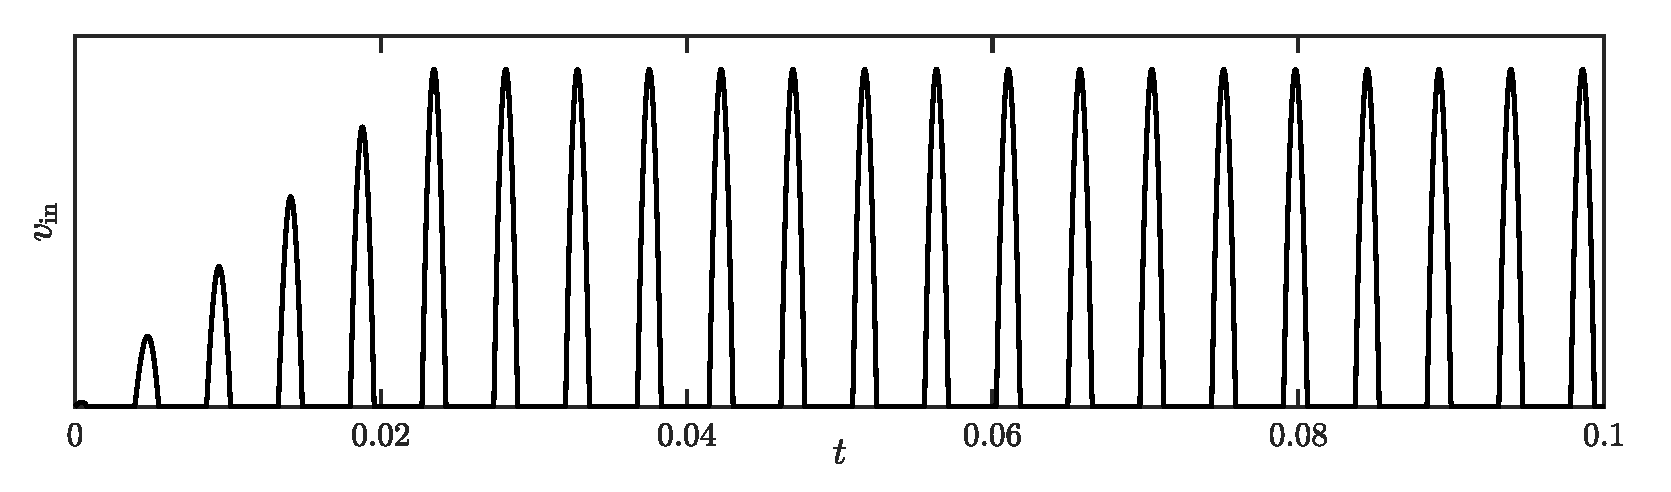
\includegraphics[width=\textwidth]{figures/resonators/brass/inputWebster.eps}
    \caption{A pulse train with a frequency of $213$ Hz. This is used to excite the implementation of Webster's equation in Section \ref{sec:outputWebster}. \label{fig:inputWebster}}
\end{figure}

% At the left boundary, one can sed $\bar S_N = S_N$ from which $S_{N+1/2}$ can be calculated:
% \begin{equation}
%     S_N = \frac{1}{2}(S_{N+1/2} + S_{N-1/2}) \ \Rightarrow \ S_{N+1/2} = 2S_N - S_{N-1/2}.
% \end{equation}
% % \begin{equation}
% %         S_0 = \frac{1}{2}(S_{1/2} + S_{-1/2}) \ \Rightarrow \  S_{-1/2}
% %         = 2S_0 - S_{1/2}
% % \end{equation}



% The same can be done for the right boundary ($\bar S_N = S_N$) if this is chosen to be anything else but open (e.g., closed or radiating -- see Section \ref{sec:radiating}):
% \begin{equation}
%     S_N = \frac{1}{2}(S_{N+1/2} + S_{N-1/2}) \ \Rightarrow \ S_{N+1/2} = 2S_N - S_{N-1/2}.
% \end{equation}
% For now though, we follow the conditions given in \eqref{eq:openClosed} and we can simply set the right boundary to its initial state
% \begin{equation}
%     \Psi_N^n = \Psi_N^0
% \end{equation}
% which is normally $0$. A more realistic open end is a radiating one, which can be found below.

\subsection{Matrix form and output}\label{sec:outputWebster}
One can write scheme \eqref{eq:discWebster} in matrix form by saving the state in a vector $\boldPsi^n = [\Psi_0^n, \hdots, \Psi_N^n]^T$ and creating a $\Dxx$ matrix that includes the effect of the cross-sectional area $S$. Assuming Neumann boundary conditions yields
\begin{equation}
    \Dxx = \frac{1}{h^2}\begin{bmatrix}
        -2& 2 &  & & & \mathbf{0}& \\
        \frac{S_{1/2}}{\Sbar_1} & -2 &\frac{S_{3/2}}{\Sbar_1} & & & & \\
        & \ddots & \ddots & \ddots &  & & \\
        & & \frac{S_{l-1/2}}{\Sbar_l}& -2 & \frac{S_{l+1/2}}{\Sbar_l} & & \\
        & & & \ddots & \ddots & \ddots & \\
        & & &  & \frac{S_{N-3/2}}{\Sbar_{N-1}}  & -2 & \frac{S_{N-1/2}}{\Sbar_{N-1}} \\
        & \mathbf{0} & & & & 2 & -2 \\
    \end{bmatrix}.
\end{equation}
Notice that there are no appearances of $S$ at the boundaries as these vanish due to the boundary conditions as in Eq. \eqref{eq:leftBoundaryWebster}.
Using $\I_N$ as the $N\times N$ identity matrix, one can write scheme \eqref{eq:discWebster} in matrix form as
\begin{equation}\label{eq:matrixFormWebsters}
    \A\boldPsi^{n+1} = \B\boldPsi^n + \C \boldPsi^{n-1} + \mathbf{v}^n
\end{equation}
where 
\begin{equation*}
    \begin{gathered}
    \A = \begin{bmatrix}
        \I_{N}& \mathbf{0}\\\
        \mathbf{0} & 1 + \alpha_+\
    \end{bmatrix}, \quad \B = 2\I + c^2 k^2 \Dxx, \quad \text{and} \quad \C = \begin{bmatrix}
        -\I_N & \mathbf{0}\\\
        \mathbf{0}& -1 + \alpha_-
    \end{bmatrix},
    \end{gathered}
\end{equation*}
and the $(N+1)\times 1$ input vector $\mathbf{v}^n$ consists of zeros except for the first index:
\begin{equation}
    \mathbf{v}_i^n = 
    \begin{cases}
        \frac{2h \lambda^2 S_{-1/2}}{\Sbar_0}v_\text{in}^n, & \text{if } i = 1,\\
        0,& \text{otherwise}.
    \end{cases}
\end{equation}
%
Notice how the radiation is included by changing the last entry of matrices $\A$ and $\C$.
The output of an implementation of Webster's equation is shown in Figure \ref{fig:outputWebster}. The parameters used for the scheme, the input signal and the geometry used to obtain the output can be found in Table \ref{tab:websterParams}, Figure \ref{fig:inputWebster}, and Figure \ref{fig:geometryWebster} respectively.
\begin{figure}[h]
    \centering
    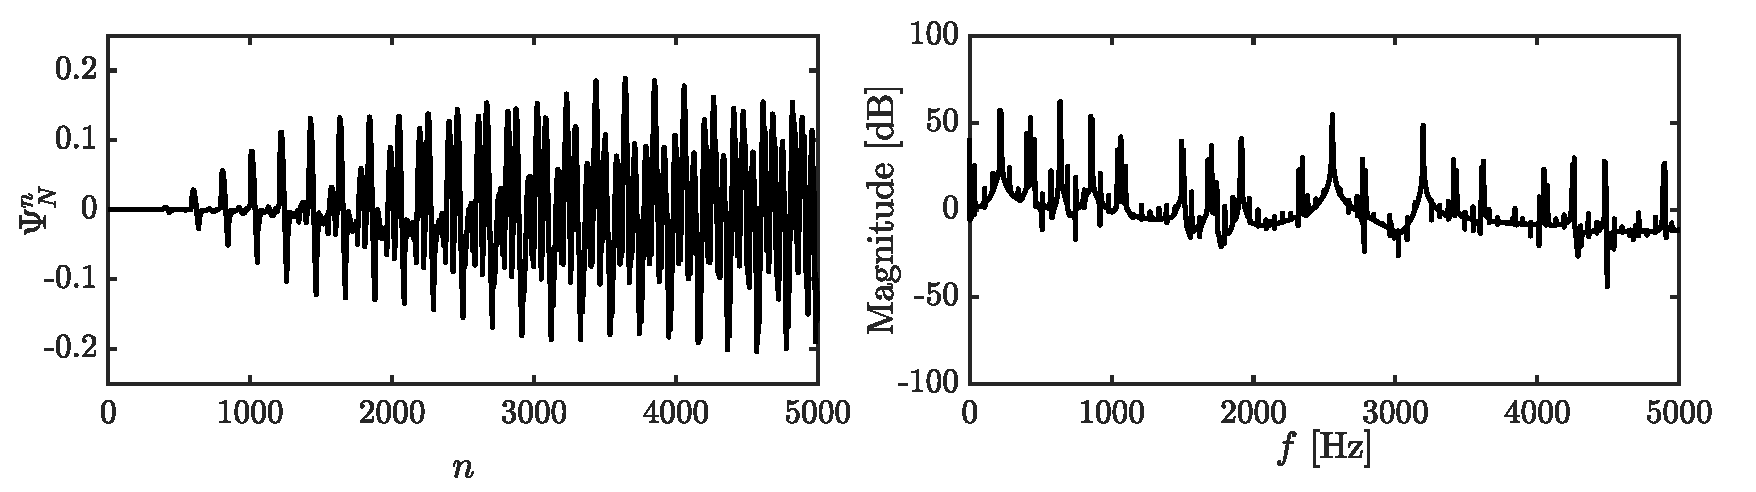
\includegraphics[width=\textwidth]{figures/resonators/brass/outputWebster.eps}
    \caption{The output of Webster's equation at $\Psi_N^n$ using the parameters in Table \ref{tab:websterParams} and geometry in Figure \ref{fig:geometryWebster}. \label{fig:outputWebster}}
\end{figure}

\begin{table}[h]
    \begin{center}
    \begin{tabular}{|l|c|c|}
        \hline
        Name & Symbol (unit) & Value\\ \hline
        Length & $L$ (m) & $\approx 3$\\
        Wave speed & $c$ (m/s) & 343\\
        Cross-sectional area & $S(x)$ & See e.g. paper \citeP[H]\\\hline
        \end{tabular}
    \caption{Parameters for the implementation of Webster's equation. The length is slightly below $3$ m to yield $\lambda = 1$ in Eq. \eqref{eq:CFLwebster}.\label{tab:websterParams}}
    \end{center}
\end{table}
{\renewcommand{\arraystretch}{1}

\hspace{0.1\textwidth}
\begin{figure}[h]
    \centering
    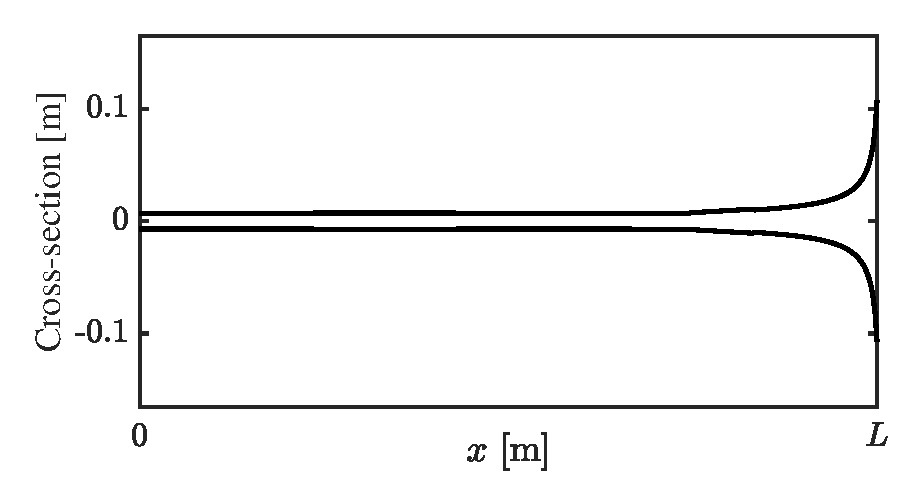
\includegraphics[width=0.6\textwidth]{figures/resonators/brass/geometryWebster.eps}
    \caption{The geometry used for the implementation. See paper \citeP[H] for more details. \label{fig:geometryWebster}}
\end{figure}


\subsection{Energy analysis}\label{sec:energyAnalysisWebster}
The energy analysis of Webster's equation with a radiating boundary might seem straightforward. However, due to the varying cross-sectional area, the energy balance deserves a more detailed treatment, especially at the boundaries. For this analysis, (centred) Neumann boundary conditions are used for both boundaries and the input is ignored. This section follows the steps presented in Section \ref{sec:energyAnalysis}.% to retain generality. %These can then easily be adapted to Dirichlet if needed.

\subsubsection{Step 1: Obtain $\dtp \h$}
Usually, to ensure vanishing boundary terms when using centred Neumann boundary conditions, the primed inner product in Eq. \eqref{eq:primedInnerProd} is chosen. However, as the system has a spatially varying cross-section, the more general \textit{weighted inner product} in Eq. \eqref{eq:weightedInnerProd} has to be chosen instead.

Taking an inner product weighted by free parameters $0 < \el, \er \leq 2$ at the left and right boundary respectively, of scheme \eqref{eq:discWebster} with $(\dtd \Psiln)$ over discrete domain $d$ yields 
\begin{equation}\label{eq:powerBalanceWebster}
    \dtp \h = \langle \dtd\Psiln ,\Sbar_l \delta_{tt}\Psi^n_l\rangle_d^{\el,\er} - c^2\langle\dtd\Psiln, \dxm(\Sp(\delta_{x+}\Psiln))\rangle_d^{\el,\er} = 0.
\end{equation}

\subsubsection{Step 2: Identify energy types and isolate $\dtp$} 
As the right boundary is set to be radiating according to Eq. \eqref{eq:centRadBound}, the energy balance will eventually be of the following form:
\begin{equation}\label{eq:radiatingEnergyForm}
    \delta_{t+}(\mathfrak{h}+\mathfrak{h}_\text{b}) = \b-\mathfrak{q}_\text{b},
\end{equation}
where $\mathfrak{h}_\text{b}$ is the energy stored by the radiating boundary through the inertia term, $\mathfrak{q}_\text{b}$ describes the the energy losses through radiation and $\b$ is the general boundary term.

% As one can rewrite
% \begin{equation}\label{eq:switchSignsWebster}
%     \dxp\left(\Sm(\delta_{x-}\Psiln)\right) \ \Longleftrightarrow\  \dxm\big(\Sp(\dxp\Psiln)\big),
% \end{equation}
Starting at Eq. \eqref{eq:powerBalanceWebster}, the last term can -- using identity \eqref{eq:weightedIdentityMinus} -- be rewritten to
\begin{equation*}
    c^2\langle\Sp \dtd \dxp \Psiln, (\dxp \Psiln)\rangle_{\underline{d}} + \b_\text{r} - \b_\text{l},
\end{equation*}
where
\begin{subequations}
    \begin{align}
     \mathfrak{b}_\text{r} &= c^2(\dtd\Psi_N^n)\left(\frac{\epsilon_\text{r}}{2}S_{N+1/2}(\dxp \Psi_N^n) + \left(1-\frac{\epsilon_\text{r}}{2}\right)S_{N-1/2}(\dxm\Psi_N^n)\right), \\
     \mathfrak{b}_\text{l} &= c^2(\dtd\Psi_0^n)\left(\frac{\epsilon_\text{l}}{2}S_{-1/2}(\dxm\Psi_0^n)+\left(1-\frac{\epsilon_\text{l}}{2}\right)S_{1/2}(\dxp \Psi_0^n))\right),
    \end{align}
\end{subequations}
are the right and left boundary term respectively (notice that $\b_\text{l}$ is subtracted). One can immediately observe that the boundary terms vanish if Dirichlet boundary conditions would be used. 
    
Then, using identities \eqref{eq:prodIdentity1} and \eqref{eq:prodIdentity2} yields 
\begin{equation*}
    \dtp \h = \b_\text{r} - \b_\text{l}
\end{equation*}
where
\begin{equation}\label{eq:energyBalanceWebster}
    \begin{gathered}
        \h = \t + \v, \qwiq \t = \frac{1}{2} \left(\lVert\sqrt{\Sbar_l} \dtm \Psiln \rVert_d^{\el, \er}\right)^2 \quad \text{and} \\
        % \v =c^2\langle\dtd \dxp \Psiln, \Sp(\dxp \Psiln)\rangle_{\underline{d}}\ .
        \v = \frac{c^2}{2}\langle \Sp\dxp \Psiln, e_{t-}\dxp\Psiln\rangle_{\underline{d}}
    \end{gathered}
\end{equation}
Notice that $\Sbar_l$ is included in the norm by using its square-root.

The next step is to find definitions for $\el$ and $\er$ such that the boundary terms vanish if radiation were to be ignored. In other words, the boundary terms need to be rewritten such that 
\begin{align*}
    \dxd \Psi_0^n &= 0\  \Rightarrow\ \b_\text{l} = 0 \\
    \dxd \Psi_N^n &= 0\  \Rightarrow\ \b_\text{r} = 0
\end{align*} 
for the left and right boundary respectively. It can be shown that, for the special cases of $\epsilon_\text{r} = S_{N-1/2}/\mu_{xx}S_N$ and $\epsilon_\text{l} = S_{1/2}/\mu_{xx}S_0$ the boundary terms vanish in this case
\begin{subequations}\label{eq:centStrictDissip}
\begin{align}
    \mathfrak{b}_\text{r} &= c^2 (\dtd\Psi_N^n)S_{N-1/2}(2-\epsilon_\text{r})(\delta_{x\cdot}\Psi_N^n)\label{eq:centStrictDissipRight},\\
    \mathfrak{b}_\text{l} &= c^2 (\dtd\Psi_0^n)S_{1/2}(2-\epsilon_\text{l})(\delta_{x\cdot}\Psi_0^n).\label{eq:centStrictDissipLeft}
\end{align}
\end{subequations}
See Appendix \ref{app:boundaryWebster} for a derivation of this. %Also note that $\el, \er \leq 2$ to the boundary terms to be non-negative. 

To add the energy stored and dissipated by the radiating boundary, its definition in Eq. \eqref{eq:centRadBound} can be substituted into the right boundary term $\b_\text{r}$ in Eq. \eqref{eq:centStrictDissipRight} as 
\begin{align*}
    \mathfrak{b}_\text{r} &= c^2 (\dtd\Psi_N^n)S_{N-1/2}(2-\epsilon_\text{r})(-a_1\dtd\Psi_N^n - a_2\mu_{t\cdot}\Psi_N^n),\\
    &= c^2 S_{N-1/2}(2-\epsilon_\text{r})\left(-a_1(\dtd\Psi_N^n)^2 - a_2(\dtd\Psi_N^n)(\mu_{t\cdot}\Psi_N^n)\right).
\end{align*}
This can then be decomposed in $\h_\text{b}$ and $\q_\text{b}$ used in Eq. \eqref{eq:powerBalanceWebster}. 
% These can be obtained by substituting the definition of the radiating boundary Eq. \eqref{eq:centRadBound} into \eqref{eq:centStrictDissipRight} to get

Using identity \eqref{eq:prodIdentity4} yields the definitions for $\h_\text{b}$ and $\q_\text{b}$ in Eq. \eqref{eq:radiatingEnergyForm}
\begin{equation}
    \h_\text{b} = \frac{c^2 S_{N-1/2}(2-\epsilon_\text{r}) a_2}{2} \mtm(\Psi_N^n)^2, \qaq \q_\text{b} = c^2 S_{N-1/2}(2-\epsilon_\text{r})a_1(\dtd\Psi_N^n)^2.
\end{equation}
Finally, $\b = \b_\text{l}$ and can be shown to vanish for both Dirichlet and (centred) Neumann conditions.

\subsubsection{Step 3: Check units}
\SWcomment[It seems like in order for the units to make sense, one must write Eq. \eqref{eq:webstersPDE} as
\begin{equation}
    \frac{S\rho}{c^2} \ptt\Psi = \frac{B}{c^2}\px(S(\px\Psi)),
\end{equation}
where $B$ is the bulk modulus of air (in N/m$^2$)]
\subsubsection{Step 4: Implementation}
Figure \ref{fig:energyWebsters} shows the energetic output of Webster's equation with a radiating boundary at $x=L$. To highlight the effect of the radiation on the energy the parameters are set to $L = 1$ and $S(x) = 0.01$ for all $x\in \D$.  The system is excited with a raised cosine close to the left boundary, and when the excitation reaches the radiating boundary, the total energy in the system decreases due to the losses. The energy stored by the boundary $\h_\text{b}$ is also shown and indeed increases when the wave reaches the boundary.
\begin{figure}[h]
    \centering
    \begin{tikzpicture}[->,node distance=3cm,
        thick,main node/.style={circle,draw}]
    
        \node[] (image) at (0,0) {
        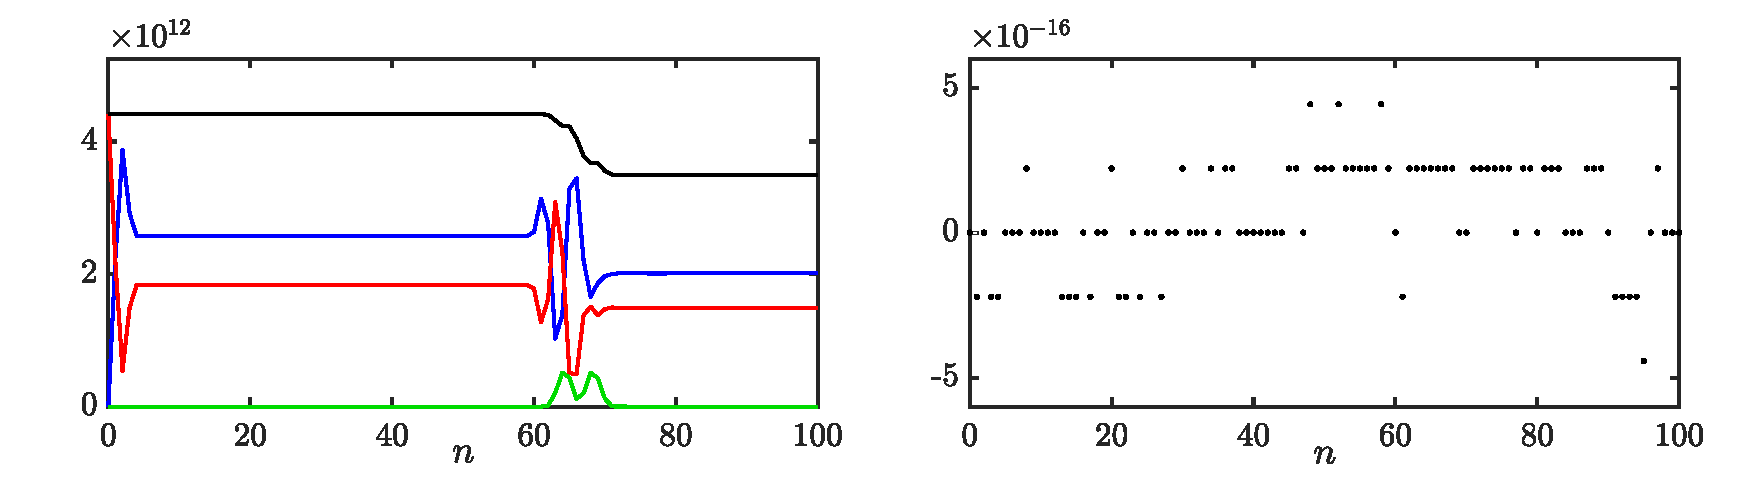
\includegraphics[width=\textwidth]{figures/resonators/brass/energyWebster2.eps}
        };
    
        \node[] (he) at (0.2,0.5) {\small $\mathfrak{h}_\text{e}$};

        \node[] (h) at (-5.75, 1) {\small $\mathfrak{h}$};
        \node[] (v) at (-5.75, 0.5) {\small $\color{red}\mathfrak{v}$};
        \node[] (t) at (-5.75, 0) {\small $\color{blue}\mathfrak{t}$};
        \node[] (hb) at (-5.75, -0.5) {\small $\color[HTML]{00DB00}\mathfrak{h}_\text{b}$};      
    \end{tikzpicture}
      \caption{The kinetic (blue), potential (red), and total (black) energy as well as the energy stored by the radiation condition (green) of an implementation of Webster's equation are plotted in the left panel. Notice that the energy decreases between $n=60$ and $n=70$ as the excitation reached the boundary where damping is included. The right panel shows the normalised energy (according to Eq. \eqref{eq:normalisedEnergyDamping}) and shows that the deviation of the energy is within machine precision. \label{fig:energyWebsters}}
\end{figure}

\subsection{Stability through energy analysis}\label{sec:stabilityEnergyWebster}
Frequency domain analysis as presented in Section \ref{sec:stabilityAnalysis}, or more specifically, von Neumann analysis, can not be performed on Webster's equation due to the varying cross-section of the system \cite{theBible}. Instead, stability conditions can be obtained through energy analysis explained in Section \ref{sec:stabilityAnalysisEnergy}.

Consider the following scheme
\begin{equation}
    [S]_l \delta_{tt}\Psi^n_l = c^2\dxm(\Sp(\delta_{x+}\Psiln)),
\end{equation}
where $[S]_l$ is a still undetermined second-order approximation to the true geometry of the acoustic tube and will be shown to be $\Sbar_l$ below. As done for the 1D wave equation in Section \ref{sec:stabilityAnalysisEnergy}, the potential energy $\v$ in Eq. \eqref{eq:energyBalanceWebster} can be rewritten using identity \eqref{eq:prodIdentityEnergyStab} as
\begin{equation*}
    \v = \frac{c^2}{2}\left(\lVert\sqrt{S_{l+1/2}}\mtm\dxp\Psiln\rVert_{\underline{d}}^2-\frac{k^2}{4}\lVert\sqrt{S_{l+1/2}}\dtm\dxp \Psiln\rVert_{\underline{d}}^2\right).
\end{equation*}
For spatially varying systems, one can use the following extension of the bound given in Eq. \eqref{eq:spatialBound} \cite{theBible}
\begin{equation}\label{eq:spatialBoundWebster}
    \lVert \sqrt{\phi_l}\dxp \uln \rVert_{\underline{d}} \leq\frac{2}{h}\lVert \sqrt{\mxm\phi_l} \uln \rVert_d,
\end{equation}
where spatially varying function $\phi_l > 0$ is defined over the same domain as $u$. The following condition can then be put on $\v$
\begin{align*}
    \v &\geq \frac{c^2}{2}\left(\lVert\sqrt{S_{l+1/2}}\mtm\dxp\Psiln\rVert_{\underline{d}}^2 - \frac{k^2}{4}\left(\frac{2}{h}\lVert\sqrt{\mxm \Sp}\dtm\Psiln\rVert_{d}\right)^2\right),\\
    &\geq \frac{c^2}{2}\left(\lVert\sqrt{S_{l+1/2}}\mtm\dxp\Psiln\rVert_{\underline{d}}^2 - \frac{k^2}{h^2}\lVert\sqrt{\mxx S_l}\dtm\Psiln\rVert_{d}^2\right)\\
    & \geq \frac{c^2}{2}\left(\lVert\sqrt{S_{l+1/2}}\mtm\dxp\Psiln\rVert_{\underline{d}}^2 - \frac{k^2}{h^2}\left(\lVert\sqrt{\mxx S_l}\dtm\Psiln\rVert_{d}^{\el,\er}\right)^2\right),
\end{align*}
where last step is possible because $0 < \el, \er \leq 2$.
% Assuming that $\el, \er \leq 2$, the following is true
% \begin{equation}
%     \lVert \uln \rVert^{\el, \er}_d\leq \lVert \uln\rVert_d
% \end{equation}
% \begin{equation}
%     \t \geq 
% \end{equation}
Substituting this into the energy balance in Eq. \eqref{eq:energyBalanceWebster} yields
\begin{align*}
    \h = \t + \v \geq &\  \frac{1}{2} \left(\lVert\sqrt{[S]_l} \dtm \Psiln \rVert_d^{\el, \er}\right)^2 \\
    &+ \frac{c^2}{2}\left(\lVert\sqrt{S_{l+1/2}}\mtm\dxp\Psiln\rVert_{\underline{d}}^2 - \frac{k^2}{h^2}\left(\lVert\sqrt{\mxx S_l}\dtm\Psiln\rVert_{d}^{\el,\er}\right)^2\right),
\end{align*}
and as $\lVert\sqrt{S_{l+1/2}}\mtm\dxp\Psiln\rVert_{\underline{d}}^2$ is non-negative, the following is also true
\begin{equation*}
    \h = \t + \v \geq \frac{1}{2} \left(\lVert\sqrt{[S]_l} \dtm \Psiln \rVert_d^{\el, \er}\right)^2- \frac{\lambda^2}{2}\left(\lVert\sqrt{\mxx S_l}\dtm\Psiln\rVert_{d}^{\el,\er}\right)^2.
\end{equation*}
This can be written as
\begin{equation}
    \h \geq \frac{1}{2} \sum_d \left(\sqrt{[S]_l} - \lambda^2\sqrt{\mxx S_l}\right)(\dtm \Psiln)^2 
\end{equation}
which is non-negative if
\begin{align*}
    \text{min}\Big(\sqrt{[S]_l} - \lambda^2\sqrt{\mxx S_l}\Big) \geq 0,\\
    \lambda \leq \text{min}\left(\sqrt{\frac{[S]_l}{\mxx S_l}}\right).
\end{align*}
For the special choice of $[S]_l = \mxx S_l$, this condition reduces to
\begin{equation}
    \lambda \leq 1,
\end{equation}
also given in \eqref{eq:CFLwebster}. This choice of $[S]_l$ is equal to $\Sbar_l$ through Eq. \eqref{eq:Sbar}, hence its choice in Eq. \eqref{eq:discWebster}.

\subsection{Modal analysis}
The variable cross-section causes the modes of the system to vary in interesting ways. If the tube is perfectly cylindrical and $S(x)$ is thus constant, Webster's equation reduces to the 1D wave equation and the modal frequencies are integer multiples of the fundamental frequency. 
For low cross-sectional variations, the modes generally follow a linear pattern. See Figure \ref{fig:webstersModes}. The damping per mode, however, follows a different pattern, where higher damping occurs around $\fs/4$, and is due to the comb-filtering effect that the radiation has on the system. \SWcomment[is this true?]

\begin{figure}[h]
    \centering
    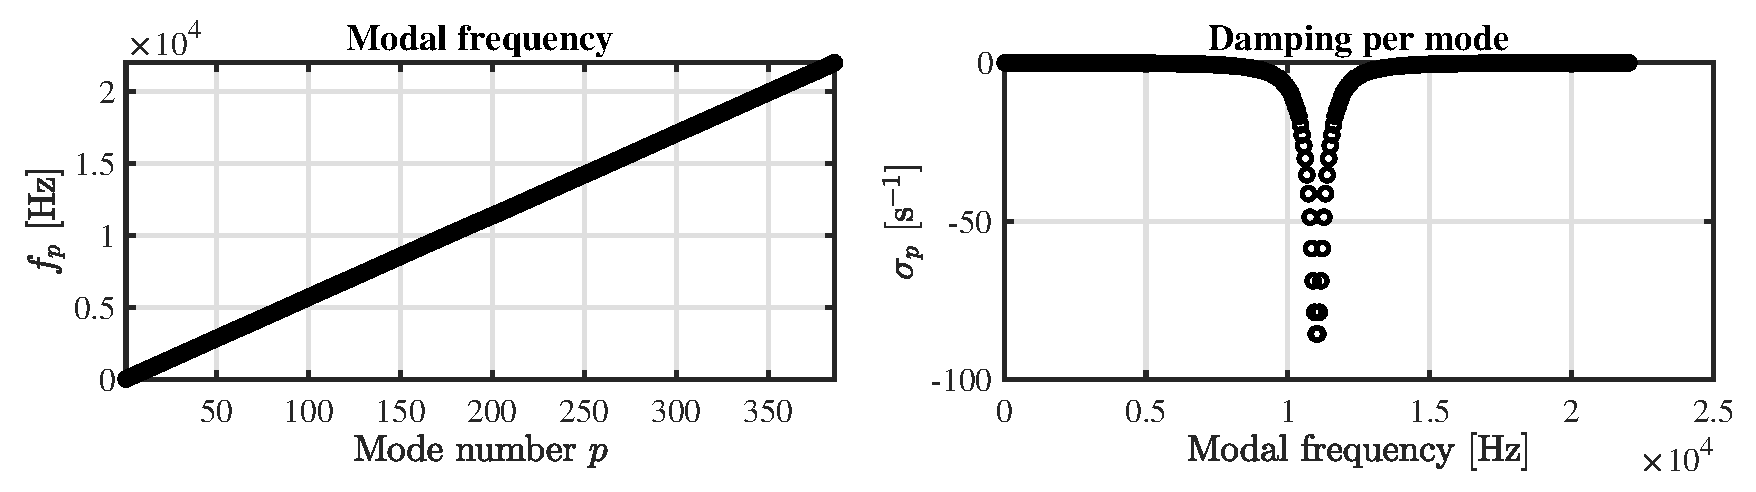
\includegraphics[width=\textwidth]{figures/resonators/brass/webstersModes.eps}
    \caption{The result of a modal analysis of Webster's equation with parameters and geometry given in \ref{sec:outputWebster}. Notice the higher damping for modes around $\fs/4$. \label{fig:webstersModes}}
\end{figure}

\section{First-order system}\label{sec:firstOrderSystem}
Until now, only PDEs  have been presented that second-order in time, i.e., that are dependent on the acceleration of the state variable. This section presents a system of two coupled first-order PDEs which are instead dependent on the velocity. State-of-the-art research on brass instruments in the context of FDTD methods also uses this coupled system (see e.g.\cite{Bilbao2016, Harrison2018}) and has been used in this project to model the trombone in paper \citeP[H].\todo{look at wording}

\subsection{Continuous time}
Using the same variables as before for cross-sectional area $S=S(x)$, wave speed $c$, and air density $\rho_0$, a system of PDEs that describes air propagation in an acoustic tube can be defined as follows:
\begin{subequations}\label{eq:firstOrderSystem}
\begin{align}
    \frac{S}{\rho_0 c^2}\partial_t p &= -\partial_x(Sv),\label{eq:contPressure}\\
    \rho_0\partial_tv &= -\partial_xp\label{eq:discVelocity},
\end{align}
\end{subequations}
where pressure $p = p(x,t)$ (Pa) and particle velocity $v = v(x,t)$ (m/s) are defined for $x\in \D$ with domain $\D = [0, L]$ and tube length $L$ (in m). These state variables are related to the acoustic potential $\Psi$ as shown in Eq. \eqref{eq:pressureVelocityWebster} as
\begin{equation}\label{eq:pressureVelocityFirstOrder}
    p = \rho_0\partial_t \Psi, \quad v = -\partial_x\Psi.
\end{equation}  
Indeed it can be shown by substituting these definitions into Eq. \eqref{eq:contPressure}, Webster's equation can be obtained:
\begin{equation}
  \nonumber
        \frac{S}{\rho_0 c^2}\partial_t(\rho_0 \partial_t\Psi) = -\partial_x(S(-\partial_x\Psi))\quad \Longrightarrow \quad S\partial_t^2\Psi = c^2\partial_x(S\partial_x\Psi).
\end{equation}


\subsubsection{Boundary conditions}
For the first-order PDE system in Eq. \eqref{eq:firstOrderSystem}, the boundary conditions are defined as follows:
\begin{subequations}
    \begin{align}\label{eq:firstOrderBoundaryConditionsCont}
        p(0,t) &= 0, &  p(L,t) &= 0, & &\quad\text{(Dirichlet, open)},\\
        S(0)v(0) &= 0, & S(L)v(L) &= 0, & &\quad \text{(Neumann, closed)},
    \end{align}
\end{subequations}
which, through Eq. \eqref{eq:pressureVelocityFirstOrder}, relate to the boundary conditions of Webster's equation in Eq. \eqref{eq:contBoundariesBrass}.

\subsection{Discrete time}
It is useful to place either $p$ or $v$ on an interleaved grid (see Figure \ref{fig:interleavedGrid}). Following \cite{Harrison2018}, $v$ is placed on this interleaved grid both in space and time. 
Accordingly, system \eqref{eq:firstOrderSystem} is discretised as
\begin{subequations}\label{eq:firstOrderFDS}
    \begin{align}
        \frac{\bar S_l}{\rho_0 c^2}\delta_{t+}p_l^n &= -\delta_{x-}(S_{l+1/2}v_{l+1/2}^{n+1/2}),\label{eq:discPressure}\\
        \rho_0 \delta_{t-}v_{l+1/2}^{n+1/2}&=-\delta_{x+}p_l^n,\label{eq:discVelocity}
    \end{align}
\end{subequations}
after which the update equations become
\begin{subequations}
    \begin{align}
        p_l^{n+1} &= p_l^n - \frac{\rho_0 c \lambda}{\bar{S}_l}(S_{l+1/2}v_{l+1/2}^{n+1/2}-S_{l-1/2}v_{l-1/2}^{n+1/2}),\label{eq:pressureUpdate}\\
        v_{l+1/2}^{n+1/2} &= v_{l+1/2}^{n-1/2}-\frac{\lambda}{\rho_0 c}(p_{l+1}^n - p_l^n),\label{eq:velocityUpdate}
    \end{align}
\end{subequations}
where (again) $\lambda = ck/h \leq 1$ for stability. The pressure is defined for $l=\{0, \hdots, N\}$ and the velocity for $l=\{0, \hdots, N-1\}$ where $N$ is the number of intervals between the grid points on the pressure grid. Notice that the range of calculation for the particle velocity is one fewer grid point than the that of the pressure.

An advantage of using an interleaved grid like this, is that the forward and backward first-order are second-order accurate, and can be shown through a Taylor series expansion as done in \ref{sec:FDoperators} (also see \cite{Harrison2018}).

\begin{figure}
    \centering
    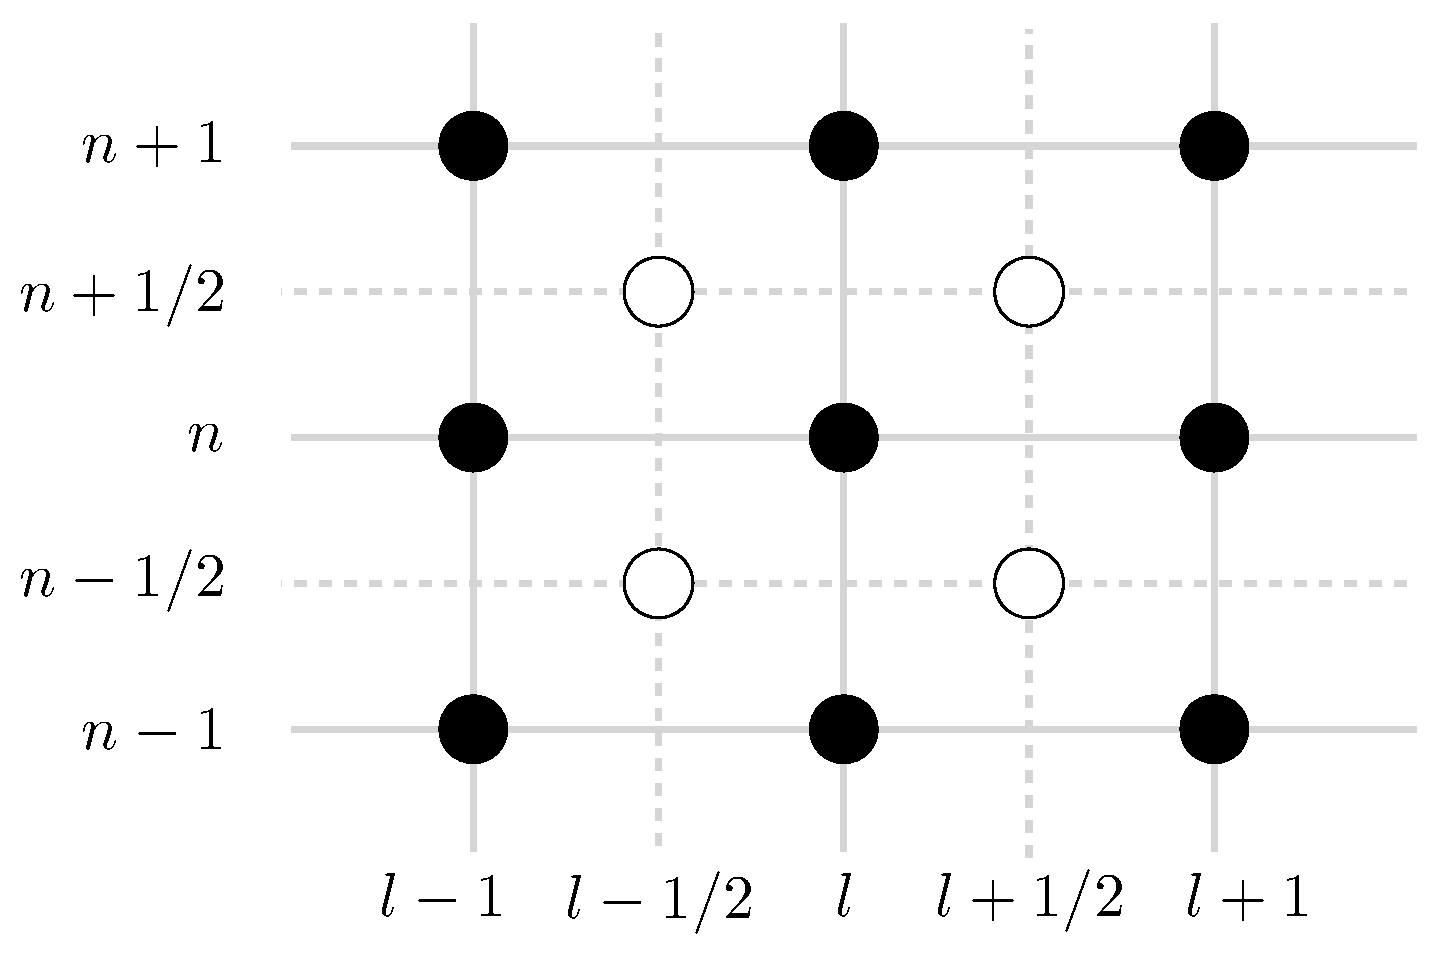
\includegraphics[width=0.7\textwidth]{figures/resonators/brass/interleavedGridFigure.pdf}
    \caption{The interleaved grid used for the system of FD schemes in Eq. \eqref{eq:firstOrderFDS}. Grid points on the regular grid (in black) are used for pressure $p$, while points on the interleaved grid (in white) are used for particle velocity $v$.\label{fig:interleavedGrid}}
\end{figure}

\subsubsection{Boundary conditions}\label{sec:boundariesFirstOrder}
The boundary conditions in Eq. \eqref{eq:firstOrderBoundaryConditionsCont} can be discretised as follows
\begin{subequations}
    \begin{align}\label{eq:firstOrderBoundaryConditions}
        p_0^n &= 0, & p_N^n &= 0, & &\text{(Dirichlet, open),}\\
        \mu_{x-}(S_{1/2}v_{1/2}^n) &= 0, & \mu_{x+}(S_{N-1/2}v_{N-1/2}^n) &= 0, & &\text{(Neumann, closed)}.
    \end{align}
\end{subequations}

\subsection{Matrix form}
System \eqref{eq:firstOrderFDS} can be written in matrix form, by saving the states of $p_l^n$ and $v_{l+1/2}^{n+1}$ in vectors as 
\begin{equation}
    \mathbf{p}^n = [p_0^n, \hdots, p_N^n]^T, \qaq \mathbf{v}^{n+1/2} = [v_{1/2}^{n+1/2}, \hdots, v_{N-1/2}^{n+1/2}]^T
\end{equation}
which are of sizes $(N+1)\times 1$ and $N\times 1$ respectively. One may then write the scheme in matrix form as  
\begin{subequations}
    \begin{align}
        \mathbf{v}^{n+1/2} &= \mathbf{v}^{n-1/2} + \B_p \mathbf{p}^n\\
        \mathbf{p}^{n+1} &= \mathbf{p}^n + \B_v \mathbf{v}^{n+1/2} 
    \end{align}
\end{subequations}
where
\begin{equation}
    \B_v = \frac{\rho_0 c}\lambda \begin{bmatrix}
        -\frac{2S_{1/2}}{\Sbar_0}& & & \mathbf{0}\\
        \frac{S_{1/2}}{\Sbar_1} & -\frac{S_{3/2}}{\Sbar_1} & & \\
        & \ddots & \ddots & \\
        & & \frac{S_{N-3/2}}{\Sbar_{N-1}} & -\frac{S_{N-1/2}}{\Sbar_{N-1}} \\
        \mathbf{0} & & & \frac{2 S_{N-1/2}}{\Sbar_N} \\
    \end{bmatrix}.
\end{equation}
is of size $(N+1) \times N$.

\begin{equation}
    \B_p = \frac{\lambda}{\rho c}\begin{bmatrix}
        1& -1& & & \mathbf{0} &\\
         & 1 & -1 & & & \\
       & & \ddots & \ddots & &\\
         & & & 1& -1& \\
        & \mathbf{0} & & & 1& -1 \\
    \end{bmatrix}.
\end{equation}
is of size $N \times (N+1)$.

Alternatively, one can write the scheme in one-step form by concatenating the states of the pressure and particle velocity into one vector. The matrix form will then be 
\begin{equation}
    \underbrace{\begin{bmatrix}
        \mathbf{p}^{n+1}\\
        \mathbf{v}^{n+1/2}
    \end{bmatrix}}_{\u^{n+1}} = \B\underbrace{\begin{bmatrix}
        \mathbf{p}^{n}\\
        \mathbf{v}^{n-1/2}
    \end{bmatrix}}_{\u^{n}} 
\end{equation}
where
\begin{equation}
    \B = \begin{bmatrix}
        \I_{N+1}+\B_v\B_p & \B_v  \\
        \B_p & \I_{N}
    \end{bmatrix},
\end{equation}
is of size $(2N + 1) \times (2N + 1)$ and may be directly used as matrix $\Q$ for the modal analysis using a one-step form described in Section \ref{sec:oneStepForm}.

Finally the concatenated vectoris defined as,
\begin{equation}
    \u^n = [p_0^n, \hdots, p_N^n, v_{1/2}^{n-1/2}, \hdots, v_{N-1/2}^{n-1/2}]^T
\end{equation}
and will be of size $(2N + 1) \times 1$. 

\subsection{Energy analysis}
This section presents an energy analysis of the first-order system presented above using the techniques presented in Section \ref{sec:energyAnalysis}. For the bulk of the analysis, \cite{Harrison2018} is followed. 

\subsubsection{Step 1: Obtain $\dtp \h$}
To obtain the correct energy balance, an inner product of Eq. \eqref{eq:discPressure} with $\mu_{t+}p_l^n$ needs to be taken over discrete domain $d = \{0, \hdots, N\}$. Using the primed inner product in Eq. \eqref{eq:primedInnerProd} and after taking all terms to the left-hand side yields\footnote{The primed rather than the weighted inner product can be used here as the eventual boundary terms can be shown to vanish when using the boundary conditions in Eq. \eqref{eq:firstOrderBoundaryConditions}.}
\begin{equation}\label{eq:firstOrderPrimed}
    \delta_{t+}\mathfrak{h} = \frac{1}{\rho_0 c^2}\langle \mu_{t+}p_l^n, \Sbar \delta_{t+}p_l^n \rangle_{d}' +\langle \mu_{t+}p_l^n, \dxm(S_{l+1/2}v_{l+1/2}^{n+1/2})\rangle_{d}' = 0.
\end{equation}


\subsubsection{Step 2: Identify energy types and isolate $\dtp$}
For the rest of the analysis, the following superscripts and subscripts will be assumed unless denoted otherwise: $n$ and $l$ for $p$, $l$ for $\bar S$, $l+1/2$ for $S$ and $l+1/2$ and $n+1/2$ for $v$. After performing summation by parts of the last term using identity \eqref{eq:summationByPartsMinusBar}, Eq. \eqref{eq:firstOrderPrimed} becomes
\begin{equation}\label{eq:discEnergyFirstOrder}
    \delta_{t+}\mathfrak{h} = \frac{1}{\rho_0 c^2}\langle \mu_{t+}p, \bar S \delta_{t+}p \rangle_{d}' -\langle \mu_{t+}\dxp p, Sv\rangle_{\underline{d}} = -\mathfrak{b} \quad \end{equation}
where the boundary term is
\begin{align}
    \mathfrak{b} &= \mathfrak{b}_\text{r} + \mathfrak{b}_\text{l}, \quad \text{with} \nonumber\\
    \mathfrak{b}_\text{r} &= (\mu_{t+}p_N)\mu_{x+}(S_{N-1/2}v_{N-1/2})\quad \text{and}\label{eq:firstOrderRightBoundary}\\
    \mathfrak{b}_\text{l} &= -(\mu_{t+}p_0)\mu_{x-}(S_{1/2}v_{1/2})\label{eq:firstOrderLeftBoundary},
\end{align}
and can be shown to vanish under the boundary conditions shown in Eq. \eqref{eq:firstOrderBoundaryConditions}. Then, Eq. \eqref{eq:discVelocity} can be substituted into Eq. \eqref{eq:discEnergyFirstOrder} to get
\begin{align}
    \delta_{t+}\mathfrak{h} &= \frac{1}{\rho_0 c^2}\langle \mu_{t+}p, \bar S \delta_{t+}p \rangle_{d}' -\langle \mu_{t+}(-\rho_0\delta_{t-}v), Sv\rangle_{\underline{d}} = 0\\
    &= \frac{1}{\rho_0 c^2}\langle \mu_{t+}p, \bar S \delta_{t+}p \rangle_{d}' + \rho_0 \langle \delta_{t\cdot}v, Sv\rangle_{\underline{d}} = 0.
\end{align}
Finally, one can use identities \eqref{eq:prodIdentity3} and \eqref{eq:prodIdentity2} for the first and second term respectively to get
\begin{equation}\label{eq:energyBalanceFirstOrder}
    \begin{gathered}
        \mathfrak{h} = \mathfrak{t} + \mathfrak{v}\quad \text{where}\\
       \mathfrak{t} = \frac{\rho_0}{2}\langle Sv, e_{t-}v\rangle_{\underline{d}}\quad \text{and} \quad \mathfrak{v} = \frac{1}{2\rho_0 c^2}\left(\lVert\sqrt{\bar S }p\rVert'_d\right)^2.
    \end{gathered}
\end{equation}
\subsubsection{Step 3: Check units}
Writing the terms in Eq. \eqref{eq:energyBalanceFirstOrder} in their units yields
\begin{align*}
    \frac{\rho_0}{2}\langle Sv, e_{t-}v\rangle_{\underline{d}}\overset{\text{in units}}{\xrightarrow{\hspace*{1cm}}}& \ \text{kg}\cdot \text{m}^{-3}\cdot \text{m} \cdot (\text{m}^2 \cdot \text{m}\cdot\text{s}^{-1} \cdot \text{m}\cdot\text{s}^{-1}),\\
    & = \text{kg} \cdot \text{m}^2 \cdot \text{s}^{-2},\\
    \frac{1}{2\rho_0 c^2}\left(\lVert\sqrt{\bar S }p\rVert'_d\right)^2\overset{\text{in units}}{\xrightarrow{\hspace*{1cm}}}&\  (\text{kg} \cdot \text{m}^{-3} \cdot \text{m}^2 \cdot \text{s}^{-2})^{-1} \cdot(\text{m} \cdot \text{kg} \cdot \text{m}^{-1}\cdot \text{s}^{-2})^2,\\
    &= \text{kg} \cdot \text{m}^2 \cdot \text{s}^{-2},
\end{align*}
and indeed have the correct units.
\subsubsection{Step 4: Implementation}
Figure \ref{fig:energyFirstOrder} shows the energetic output of an implementation of the first order system in Eq. \eqref{eq:firstOrderFDS}, and shows that the energy is within machine precision.

\begin{figure}[h]
    \centering
    \begin{tikzpicture}[->,node distance=3cm,
        thick,main node/.style={circle,draw}]
    
        \node[] (image) at (0,0) {
        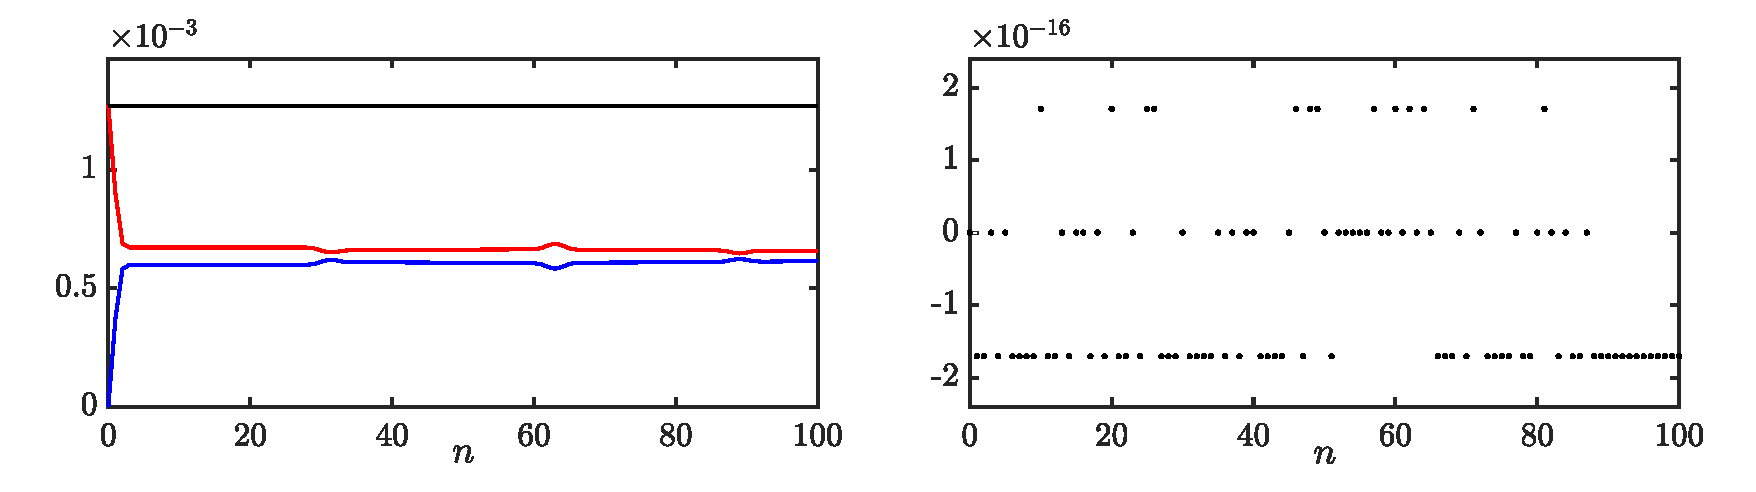
\includegraphics[width=\textwidth]{figures/resonators/brass/energyFirstOrder.eps}
        };
    
        \node[] (he) at (0.2,0.5) {\small $\mathfrak{h}_\text{e}$};

        \node[] (h) at (-5.75, 1) {\small $\mathfrak{h}$};
        \node[] (v) at (-5.75, 0.5) {\small $\color{red}\mathfrak{v}$};
        \node[] (t) at (-5.75, 0) {\small $\color{blue}\mathfrak{t}$};
    \end{tikzpicture}
      \caption{The kinetic (blue), potential (red), and total (black) energy of an implementation of the first-order system in Eq. \eqref{eq:firstOrderFDS} are plotted in the left panel. The right panel shows the normalised energy (according to Eq. \eqref{eq:normalisedEnergy}) and shows that the deviation of the energy is within machine precision. \label{fig:energyFirstOrder}}
\end{figure}

\subsection{Adding radiation}
\def\r{\text{r}}
\def\one{{(1)}}
Following \cite{Harrison2018}, radiation  can be added to the schemes using a circuit representation of the Levine and Schwinger radiation model (See Figure \ref{fig:circuit}). This section will provide a derivation \SWcomment[I'll actually move most of this to an appendix...]

\begin{figure}[h]
    \centering
    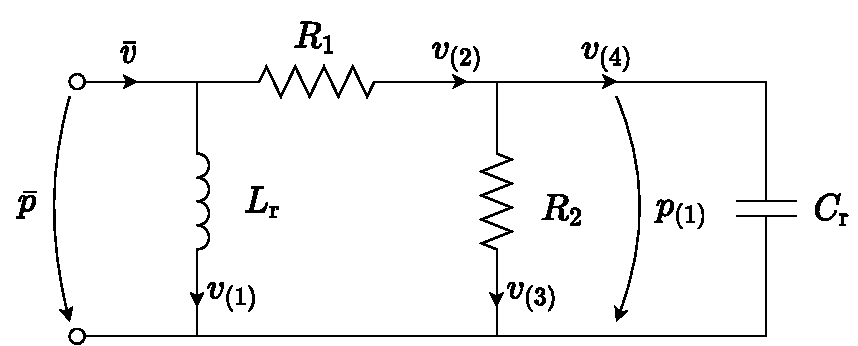
\includegraphics[width=0.7\textwidth]{figures/resonators/brass/circuit.pdf}
    \caption{The circuit representation of the Levine and Schwinger radiation model. \label{fig:circuit}}
\end{figure}

The system can be described as
\begin{subequations}\label{eq:barVPSystem}
    \begin{align}
        \bar v &= \mu_{t+}v_\one + \frac{1}{R_2}\mu_{t+}p_\one + C_\r \delta_{t+}p_\one,\label{eq:barV}\\
        \bar p &= L_\r \delta_{t+}v_\one,\label{eq:barP1}\\
        \bar p &= \left(1+\frac{R_1}{R_2}\right)\mu_{t+}p_\one+ R_1 C_\r\delta_{t+}p_\one\label{eq:barP2},
    \end{align}
\end{subequations}
where $\bar p^{n+1/2}$ and $\bar v^{n+1/2}$ are placed on the interleaved temporal grid and are related to the tube by
\begin{equation}\label{eq:barVars}
    \bar p = \mu_{t+}p^n_N, \quad \bar S_N \bar v = \mu_{x-}\left(S_{N+1/2}v_{N+1/2}^{n+1/2}\right).
\end{equation}
This can applied to the right boundary of the tube by evaluating Eq. \eqref{eq:pressureUpdate} at $l = N$
\begin{equation}
    p_N^{n+1} = p_N^n - \frac{\rho_0 c \lambda}{\bar{S}_N}\left(S_{N+1/2}v_{N+1/2}^{n+1/2}-S_{N-1/2}v_{N-1/2}^{n+1/2}\right),
\end{equation}
and, rewriting this to 
\begin{align}
    p_N^{n+1} &= p_N^n - \frac{\rho_0 c \lambda}{\bar{S}_N}\left(2\mu_{x-}\left(S_{N+1/2}v_{N+1/2}^{n+1/2}\right)-2S_{N-1/2}v_{N-1/2}^{n+1/2}\right)\nonumber,\\
    p_N^{n+1} &= p_N^n - \frac{2\rho_0 c \lambda}{\bar{S}_N}\left(\bar S_N \bar v-S_{N-1/2}v_{N-1/2}^{n+1/2}\right)\label{eq:preSolutP}.
\end{align}
A definition for $\bar v$ can then be found by first expanding Eq. \eqref{eq:barV} to 
\begin{equation}\label{eq:vBarExpanded}
    \bar v = \frac{1}{2}\left(v_\one^{n+1} + v_\one^n\right) + \left(\frac{1}{2R_2} + \frac{C_\r}{k}\right) p_\one^{n+1} +\left(\frac{1}{2R_2} - \frac{C_\r}{k}\right)p_\one^n.
\end{equation}
The goal is to make this definition solely dependent on the known values $v_\one^n$, $p_\one^n$ and $p_N^n$ and the unknown $p_N^{n+1}$ (as this can be obtained using Eq. \eqref{eq:preSolutP}).

Equation \eqref{eq:barP1} can be expanded to 
\begin{equation}\label{eq:voneNext}
    v_\one^{n+1} = \frac{k}{L_\r}\bar p + v_\one^n ,
\end{equation}
and Eq. \eqref{eq:barP2} to 
\begin{align*}
    &\bar p =\left(1+\frac{R_1}{R_2}\right)\mu_{t+}p_\one+ R_1 C_\r\delta_{t+}p_\one,\\
    &\bar p =\frac{1}{2}\left(1+\frac{R_1}{R_2}\right)\left(p_\one^{n+1} + p_\one^n\right) + \frac{R_1C_\r}{k}\left(p_\one^{n+1} - p_\one^n\right),\\
    \left(\frac{1}{2}+\frac{R_1}{2R_2} + \frac{R_1C_\r}{k}\right)&p_\one^{n+1} = \bar p + \left(\frac{R_1C_\r}{k} - \frac{1}{2} - \frac{R_1}{2R_2}\right)p_\one^n
\end{align*}
and finally solved for $p_\one^{n+1}$ as
\begin{equation}\label{eq:poneNext}
    p_\one^{n+1} = \underbrace{\left(\frac{2R_2k}{2R_1R_2C_\r + k(R_1 + R_2)}\right)}_{\zeta_1}\bar p + \underbrace{\left(\frac{2R_1R_2C_\r - k(R_1 + R_2)}{2R_1R_2C_\r + k(R_1 + R_2)}\right)}_{\zeta_2} p_\one^n .
\end{equation}
Equations \eqref{eq:voneNext} and \eqref{eq:poneNext} can then be substituted into Eq. \eqref{eq:vBarExpanded} and using the definition of $\bar p$ from Eq. \eqref{eq:barVars} yields
\begin{align}
    \bar v &= \frac{1}{2}\left(\frac{k}{L_\r}(\mu_{t+}p_N^n) + 2v_\one^n\right)+\left(\frac{1}{2R_2} + \frac{C_\r}{k}\right)\zeta_1\mu_{t+}p_N^n\nonumber \\
    & \qquad\qquad+ \left(\frac{1}{2R_2} + \frac{C_\r}{k}\right)\zeta_2p_\one^n + \left(\frac{1}{2R_2} - \frac{C_\r}{k}\right)p_\one^n\nonumber,\\
    \bar v &= \underbrace{\left(\frac{k}{2L_\r} + \frac{\zeta_1}{2R_2}+\frac{C_\r\zeta_1}{k}\right)}_{\zeta_3}\mu_{t+}p_N^n + v_\one^n + \underbrace{\left(\frac{\zeta_2+1}{2R_2} + \frac{C_\r\zeta_2 - C_\r}{k}\right)}_{\zeta_4}p_\one^n.
\end{align}
Finally, substituting this definition for $\bar v$ into Eq. \eqref{eq:preSolutP} yields
\begin{align}
    p_N^{n+1} &= p_N^n - \frac{2\rho_0c\lambda}{\bar S_N}\left(\bar S_N
    \left[\zeta_3\left(\frac{p_N^{n+1} + p_N^n}{2}\right) + v_\one^n + \zeta_4p_\one^n\right] - S_{N-1/2}v_{N-1/2}^{n+1/2}\right)\nonumber\\
    p_N^{n+1} &= p_N^n - \rho_0c\lambda\left(\zeta_3(p_N^{n+1} + p_N^n) + 2(v_\one^n + \zeta_4p_\one^n)-\frac{2S_{N-1/2}v_{N-1/2}^{n+1/2}}{\bar S_N}\right)\nonumber
\end{align}
and yields a definition for $p_N^{n+1}$ based on known values of the system 
\begin{equation}
    p_N^{n+1} = \frac{1 - \rho_0c\lambda\zeta_3}{1+\rho_0c\lambda\zeta_3}p_N^n - \frac{2\rho_0c\lambda}{1+\rho_0c\lambda\zeta_3} \left( v_\one^n+\zeta_4p_\one^n - \frac{S_{N-1/2}v_{N-1/2}^{n+1/2}}{\bar S_N}\right).
\end{equation}
\subsection{Energy}
\SWcomment[not done yet...]
Recalling the condition at the right boundary from \eqref{eq:firstOrderRightBoundary}
\begin{equation}
    \mathfrak{b}_\r = (\mu_{t+}p_N)\underbrace{\mu_{x+}(S_{N-1/2}v_{N-1/2})}_{\mu_{x-}S_{N+1/2}v_{N+1/2}},
\end{equation}
using Eq. \eqref{eq:barVars} one can rewrite this to
\begin{equation}
    \mathfrak{b}_\r = \bar p\bar S_N\bar v.
\end{equation}
then we can 


\part{Exciters}\label{part:exciters}
\chapter*{Resonators}
<<<<<<< HEAD
Though the physical models described in the previous part are also considered resonators, they are \textit{ideal} cases. In other words, you would not be able to find these ``in the wild'' as they do not includes effects such as losses or frequency dispersion. 

This part presents the different resonators used over the course of the project and is structured as follows: Chapter \ref{ch:stiffString} introduces the stiff string, a model which has been used a lot over the course of this project, Chapter \ref{ch:brass} talks about brass instruments, or more generally, 1D systems of varying geometry along their spatial dimension. Finally, Chapter \ref{ch:2Dsyst} will introduces 2D systems which, in this project, have been used to simulate (simplified) instrument bodies.
=======
Although the physical models described in the previous part -- the simple mass-spring system and the 1D wave equation -- are also considered resonators, they are \textit{ideal} cases. In other words, these can not be found in the real world as effects such as losses or frequency dispersion are not included. 

This part presents the different resonators used over the course of the project that better include these non-ideal physical processes and is structured as follows: Chapter \ref{ch:stiffString} introduces the stiff string, an extension of the 1D wave equation, % and is the single most-used model in this project. 
Chapter \ref{ch:brass} introduces acoustic tubes, used to model brass instruments, and finally, Chapter \ref{ch:2Dsyst} introduces 2D systems which, in this project, have been used to simulate (simplified) instrument bodies. The analysis techniques introduced in the previous part will be applied to all models and described in detail. 
>>>>>>> master

% \chapter{Unmodelled Excitations}\todo{Different title here?}

\section{Initial conditions}

\subsubsection{Hammer}
Full raised cosine

\subsubsection{Pluck}
\begin{itemize}
    \item Cut-off raised cosine
    \item Triangle (for string)
\end{itemize}


\section{Signals}
\subsection{Pulse train}
For brass

\subsection{Noise}
Noise input

\chapter{Excitations}\label{ch:excitations}

\section{Unmodelled excitations}

\subsection{Impulse}
The simplest way of exciting a system is to add an impulse to 
\subsection{The raised cosine}


\subsubsection{Pluck}
\begin{itemize}
    \item Cut-off raised cosine
    \item Triangle (for string)
\end{itemize}

\subsection{Signals}
\subsubsection{Pulse train}
For brass

\subsubsection{Noise}
Noise input

\section{Preamble: Newton-Raphson}\label{sec:newtonRaphson}
Before moving on to more complex excitation mechanisms, it is useful to go over the process of how to solve some of these. 
Iterative root-finding method that finds answers to nonlinear equations. 

\subsection{Mass-spring Systems Revisited: Adding Damping}

Damping can be added to Eq. \eqref{eq:massSpringPDE}  
\begin{equation}
    M\ddot u = -Ku - R\dot u
\end{equation}
with damping coefficient $R$ (in kg/s). To this system we can add an external force:
\begin{equation}
    M\ddot u = -Ku - R\dot u + F
\end{equation}
where 
\section{The Bow}
The bow

Excites the system with a force due to friction, which has a nonlinear relationship to the relative velocity between the bow and the string. 



Helmholtz motion..

\begin{figure}[h]
    \centering
    \begin{tikzpicture}[->,node distance=3cm,
        thick,main node/.style={circle,draw}]
    
        \node[] (image) at (0,0) {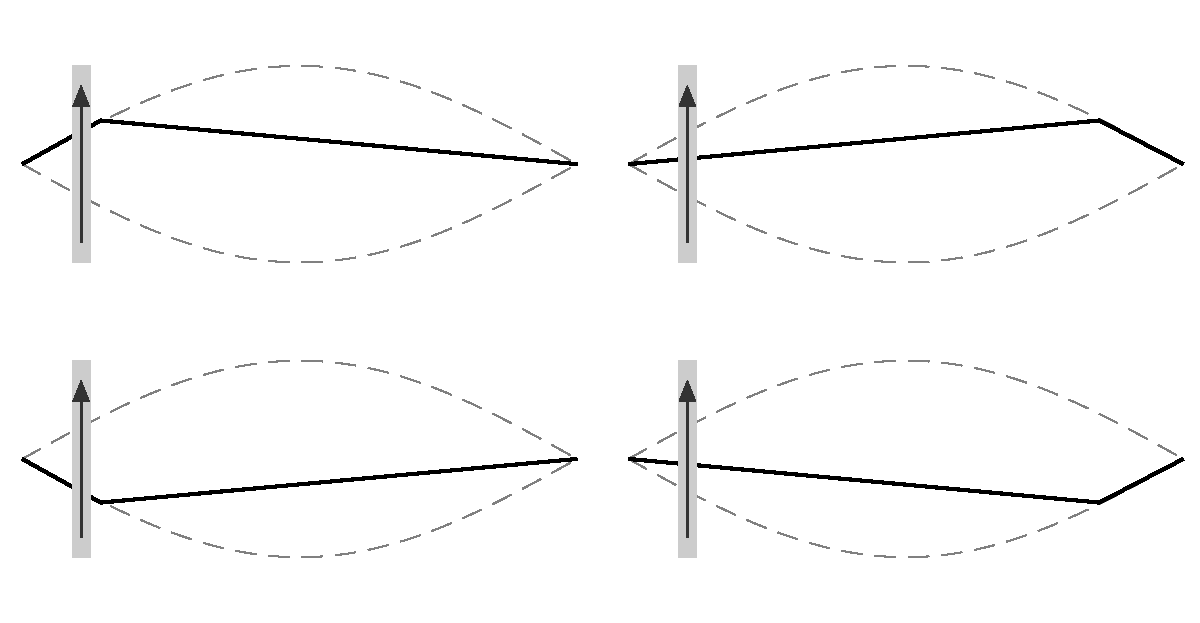
\includegraphics[width=1\columnwidth]{figures/exciters/helmholtz.eps}};
    
        \draw[thick, ->] (-0.25,0.60) arc (110:430:0.6);
        
      \end{tikzpicture}
    \caption{Helmholtz motion. \label{fig:helmholtz}}
\end{figure}

coined as `stick-slip' motion by Bowden and Leben in 1939 \cite{Bowden1939}

See fx. \url{https://www.youtube.com/watch?v=6JeyiM0YNo4}

Characteristic triangular motion (wave shapes?)

\subsection{Static Friction Models}
In static bow-string-interaction models, the friction force is defined as a function of the relative velocity between the bow and the string only.
The first mathematical description of friction was proposed by Coulomb in 1773 \cite{Coulomb1773}\todo{check references here} to which static friction, or \textit{stiction}, was added by Morin in 1833 \cite{Morin1833} and viscous friction, or velocity-dependent friction, by Reynolds in 1886 \cite{Reynolds1886}. In 1902, Stribeck found a smooth transition between the static and the coulomb part of the friction curve now referred to as the Stribeck effect \cite{Stribeck1902}. The latter is still the standard for static friction models today.

In this project, only the following static friction model has been used \cite{theBible}

\begin{equation}\label{eq:frictionCharacteristic}
    \Phi (\vrel) = \sqrt{2a}\vrel e^{-a\vrel^2 + 1/2}
\end{equation}

\todo{FULL DOC SWEEP: check figure centering}\begin{figure}[h]
    \centering
    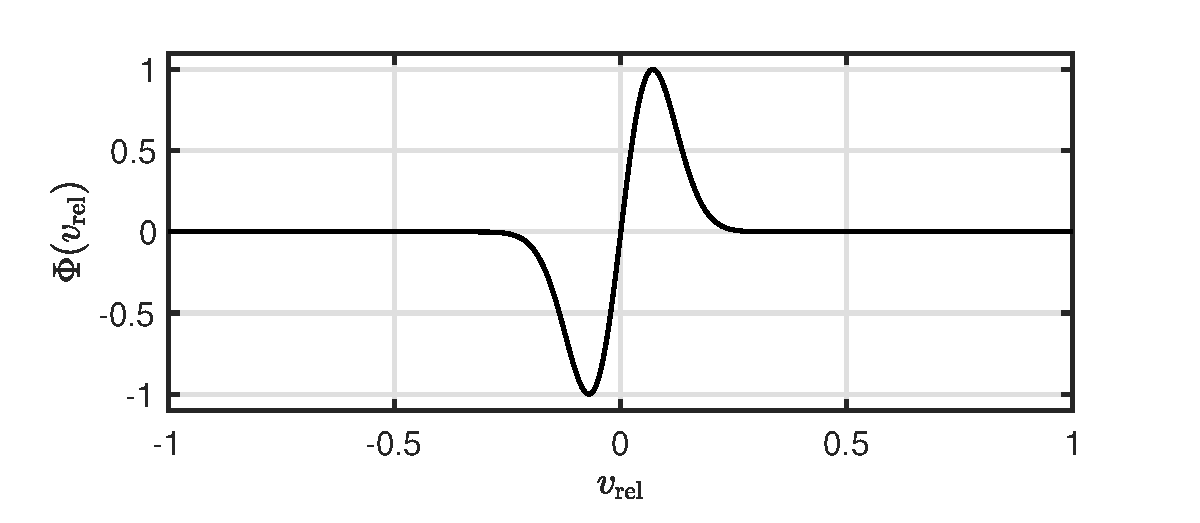
\includegraphics[width=0.8\textwidth]{figures/exciters/frictionCharacteristic.eps}
    \caption{The friction characteristic in \eqref{eq:frictionCharacteristic} with $a = 100$. \label{fig:frictionCharacteristic}}
\end{figure}

\subsection{Dynamic Friction Models}
As opposed to less complex bow models, such as the hyperbolic [source] and exponential [source] models, the elasto-plastic bow model assumes that the friction between the bow and the string is caused by a large quantity of bristles, each of which contributes to the total amount of friction.

Dynamic friction models exhibit \SWcomment[/ model] \textit{hysteresis}: the dependence of a system on its history. 
\begin{figure}[ht]
    \centering
    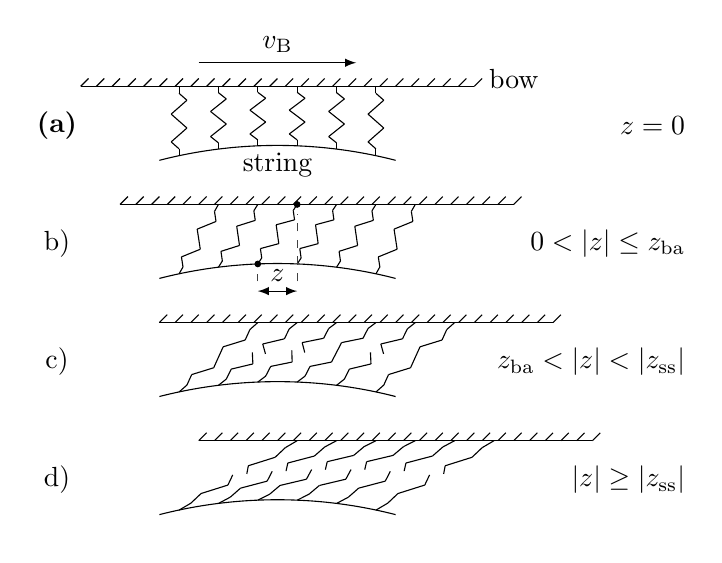
\begin{tikzpicture}
    
    \def\radius{6}; % Radius of the string (>2!)
    \pgfmathsetmacro{\reps}{3}; % How may back-and-forths in the drawing of the springs
    \def\horShift{0.5}; %how far the bow is shifted to the right in b)
    \def\bowSpacing{0.2};
    \def\drawingSpacing{1.5}
    \def\bowWidth{5};
    
    %subfigure letters
    \node (A) at (-2.8, 0.5) {\textbf{(a)}};
    \node (B) at (-2.8, 0.5 - \drawingSpacing) {b)};
    \node (C) at (-2.8, 0.5 - \drawingSpacing * 2) {c)};
    \node (D) at (-2.8, 0.5 - \drawingSpacing * 3) {d)};
    
    %bow velocity arrow
    \draw[->] (-1, 1.3) -- (1, 1.3) node [midway, above] (velText) {$v_\text{B}$};
    
    \pgfmathsetmacro{\zCoordTop}{0};
    \pgfmathsetmacro{\zYCoordBottom}{0};
    \def\springForZ{2}
    \foreach \drawing in {0, ..., 3}
    {
        %% Draw String
        \begin{scope}
            \clip (-1.5,-0.2- \drawing * \drawingSpacing) rectangle (1.5,1.5);
            \draw (0,-\radius + 0.25 - \drawing * \drawingSpacing) circle(\radius);
        \end{scope}

        %% Draw Bow
        \def\halfBW{\bowWidth*0.5}
        \pgfmathsetmacro{\halfNumDiag}{0.5 * \bowWidth / \bowSpacing};
        \draw[-] (-\halfBW + \drawing * \horShift,1 - \drawing * \drawingSpacing) -- (\halfBW + \drawing * \horShift, 1 - \drawing * \drawingSpacing);
        \foreach \bowDiag in {-\halfNumDiag, ...,\halfNumDiag}
        {
        \pgfmathtruncatemacro{\bD}{\bowDiag}
        % \ifnum\drawing=0
        %     \ifnum\bD<-1
        %         \draw[-] (\drawing * \horShift + \bowDiag * \bowSpacing, -\drawing * \drawingSpacing + 1) -- (\drawing * \horShift + \bowDiag * \bowSpacing + 0.1, -\drawing * \drawingSpacing + 0.1 + 1);
        %         \else
        %         \ifnum\bD>1
        %             \draw[-] (\drawing * \horShift + \bowDiag * \bowSpacing, -\drawing * \drawingSpacing + 1) -- (\drawing * \horShift + \bowDiag * \bowSpacing + 0.1, \drawing * -2 + 0.1 + 1);
        %         \fi
        %     \fi
        % \else
            \draw[-] (\drawing * \horShift + \bowDiag * \bowSpacing, -\drawing * \drawingSpacing + 1) -- (\drawing * \horShift + \bowDiag * \bowSpacing + 0.1, -\drawing * \drawingSpacing + 0.1 + 1);
        % \fi
            
        }
        
        \def\brokenSprings{{0, 1, 1, 0, 1, 0}};
        %% Draw Springs
        \foreach \springNo in {0, ..., 5}
        {
            % Calculate spring length depending on the radius of the string
            \pgfmathsetmacro{\startX}{\springNo  * 0.5 - 1.25};
            \pgfmathsetmacro{\calcSpace}{(\radius + 1) - \radius * sin(acos(\startX/\radius)) - 0.25};
            \pgfmathsetmacro{\springLength}{sqrt(\calcSpace*\calcSpace+\drawing*\horShift*\drawing*\horShift)};
            
            \pgfmathsetmacro{\spacing}{\springLength / (\reps + 2)}; 
            % spacing between two spring-back-and-forths
            \ifnum\drawing=0
                \pgfmathsetmacro{\rot}{0};
            \else
                \pgfmathsetmacro{\rot}{(270+(atan(\calcSpace/(\drawing*\horShift))))}; %rotation of the springs
            \fi
            
            \ifnum\drawing=1
                \ifnum\springNo=\springForZ
                    \pgfmathsetmacro{\resTwo}{sqrt(\springLength*\springLength-\horShift*\horShift)};
                    \global\let\zCoordBottom = \resTwo;
                \fi
            \fi
        
            \pgfmathsetmacro{\isBroken}{\brokenSprings[\springNo]};
            % debug code
            % \node (nodeTest\springNo) at (\springNo*1.1-2, -3 - 1 * \drawing + 0.3 * \springNo) {\isBroken};
            
            \begin{scope}[shift={(\startX + \drawing * \horShift,1 -\drawing * \drawingSpacing)}]
                \pgfmathsetmacro{\xWidth}{0.1 - (\drawing * 0.02)};
                \draw[-, rotate = \rot] (0, 0) -- (0, -\spacing * 0.5);
                \draw[-, rotate = \rot] (0, -\spacing * 0.5) -- (\xWidth, -\spacing);
                \def\Y{-\spacing}
                \foreach \idx in {1,...,\reps}
                {
                    \pgfmathsetmacro{\idxMinOne}{\idx-1};
                    \ifnum\drawing=2
                        \ifnum\isBroken=1
                            \pgfmathtruncatemacro{\idxT}{\reps * 0.5 + 1}
                            \ifnum\idx=\idxT
                                \draw[-, rotate = \rot] (\xWidth, \Y - \idxMinOne * \spacing) -- (-\xWidth,\Y - \idx * \spacing*0.6);
                                \draw[-, rotate = \rot] (\xWidth, \Y - \idxMinOne * \spacing * 1.66) -- (-\xWidth,\Y - \idx * \spacing);
                            \else
                                \draw[-, rotate = \rot] (\xWidth, \Y - \idxMinOne * \spacing) -- (-\xWidth,\Y - \idx * \spacing);
                            \fi
                        \else
                                \draw[-, rotate = \rot] (\xWidth, \Y - \idxMinOne * \spacing) -- (-\xWidth,\Y - \idx * \spacing);
                        \fi
                    \else
                        \ifnum\drawing=3
                            \pgfmathtruncatemacro{\idxT}{\reps * 0.5 + 1}
                            \ifnum\idx=\idxT
                                \draw[-, rotate = \rot] (\xWidth, \Y - \idxMinOne * \spacing) -- (-\xWidth,\Y - \idx * \spacing*0.6);
                                \draw[-, rotate = \rot] (\xWidth, \Y - \idxMinOne * \spacing * 1.66) -- (-\xWidth,\Y - \idx * \spacing);
                            \else
                                \draw[-, rotate = \rot] (\xWidth, \Y - \idxMinOne * \spacing) -- (-\xWidth,\Y - \idx * \spacing);
                            \fi
                        \else
                            \draw[-, rotate = \rot] (\xWidth, \Y - \idxMinOne * \spacing) -- (-\xWidth,\Y - \idx * \spacing);
                        \fi
                    \fi
                    \pgfmathsetmacro{\invXWidth}{\xWidth*-1};
                    \global\let\xWidth = \invXWidth;
                    \pgfmathsetmacro{\lastYPre}{\Y - \idx * \spacing};
                    \global\let\lastY = \lastYPre;
                }
                \draw[-, rotate = \rot] (\xWidth, \lastY) -- (0, \lastY - \spacing * 0.5);
                \draw[-, rotate = \rot] (0, \lastY - \spacing * 0.5) -- (0, \lastY - \spacing);
             \end{scope}
             
        }
        % \draw[<->] (2,2-0.707) -- node[right] {$r=\sqrt{2} \Rightarrow A=\pi(\sqrt{2})^2=2\pi$} (2,2+0.707);
        
        % \node(stringText) at (0, -\drawing * 2) {string};
        % \node[block, minimum height = 0.15cm, fill=white, draw=white] (bowText) at (\drawing * \horShift, 1.23 - \drawing * 2) {bow};
    }
    \filldraw[black] (-1.25+\springForZ*0.5 + \horShift,1-\drawingSpacing) circle (1pt) node[anchor=center](topZ){};
    \filldraw[black] (-1.25++\springForZ*0.5,1-\zCoordBottom-\drawingSpacing) circle (1pt) node[anchor=center](bottomZ){};
    
    \node [](leftNode) at (-1.25+\springForZ*0.5,-\drawingSpacing - 0.1) {};
    \node [](rightNode) at (-1.25 +\springForZ*0.5 + \horShift,-\drawingSpacing - 0.1) {};
    
    \draw[<->] (leftNode.center) -- (rightNode.center) node [midway, above] (TextNode) {$z$};
    \draw[dashed, darkgray] (leftNode) -- (bottomZ);
    \draw[dashed, darkgray] (rightNode) -- (topZ);
    %% Draw bow and string texts
        \node(stringText) at (0, 0) {string};
        \node(bowText) at (3, 1.1) {bow};
    %% Draw descriptions of z
    \def\zTexts{{"$z=0$", "$0<|z|<z_{\text{ba}}$", "$z_{\text{ba}}<|z|< z_\text{ss}$", "$|z|>z_\text{ss}$"}};
    
    \node[anchor = east](zText1) at (5.3, 0.5) {$z=0$};
    \node[anchor = east](zText1) at (5.3, 0.5 - \drawingSpacing) {$0<|z|\leq z_{\text{ba}}$};
    \node[anchor = east](zText1) at (5.3, 0.5 - \drawingSpacing * 2) {$z_{\text{ba}}<|z|< |z_\text{ss}|$};
    \node[anchor = east](zText1) at (5.3, 0.5 - \drawingSpacing * 3) {$|z|\geq|z_\text{ss}|$};
    
    \end{tikzpicture}
    \caption{\it Microscopic displacements of the bristles between the bow and the string. The bow moves right with a velocity of $v_\text{B}$. (a) The initial state is where the average bristle displacement $z=0$. (b) The bow has moved right relative to the string. The purely elastic, or presliding regime is entered (stick). (c) After the break-away displacement $z_\text{ba}$, more and more bristles start to `break'. This is defined as the elasto-plastic regime. (d) After all bristles have `broken', the steady state (slip) is reached and the purely plastic regime is entered. (Taken from \citeP[C].)\SWcomment[exactly the same caption as paper]}
    \label{fig:elastoPlastic}
\end{figure}

\section{Lip-reed}
Lip-reed model



Coupling to Tube


\part{Interactions}\label{part:interactions}
\chapter*{Resonators}
<<<<<<< HEAD
Though the physical models described in the previous part are also considered resonators, they are \textit{ideal} cases. In other words, you would not be able to find these ``in the wild'' as they do not includes effects such as losses or frequency dispersion. 

This part presents the different resonators used over the course of the project and is structured as follows: Chapter \ref{ch:stiffString} introduces the stiff string, a model which has been used a lot over the course of this project, Chapter \ref{ch:brass} talks about brass instruments, or more generally, 1D systems of varying geometry along their spatial dimension. Finally, Chapter \ref{ch:2Dsyst} will introduces 2D systems which, in this project, have been used to simulate (simplified) instrument bodies.
=======
Although the physical models described in the previous part -- the simple mass-spring system and the 1D wave equation -- are also considered resonators, they are \textit{ideal} cases. In other words, these can not be found in the real world as effects such as losses or frequency dispersion are not included. 

This part presents the different resonators used over the course of the project that better include these non-ideal physical processes and is structured as follows: Chapter \ref{ch:stiffString} introduces the stiff string, an extension of the 1D wave equation, % and is the single most-used model in this project. 
Chapter \ref{ch:brass} introduces acoustic tubes, used to model brass instruments, and finally, Chapter \ref{ch:2Dsyst} introduces 2D systems which, in this project, have been used to simulate (simplified) instrument bodies. The analysis techniques introduced in the previous part will be applied to all models and described in detail. 
>>>>>>> master

\chapter{Collisions}\label{ch:collisions}
Something about collisions
\section{Classic models}

\section{Michele's tricks}
\chapter{Connections}\label{ch:connections}


Although briefly mentioned in the previous chapter in Section \ref{sec:twoSidedCollision}, \todo{CONNECTION COLLISION}

One can use connections to simulate a point-like damping finger on a string to create different pitches.

Pointlike $\delta(x-x_\ctxt)$ or distributed $E_\ctxt$

When connecting systems, notation becomes extremely important. Subscripts will be extensively used throughout this chapter to denote what variables belong to what system. Although this results in something of a notational jungle, it is better to be explicit and avoid confusion. 

\cite{Bilbao2009Modular} presents a way to explicitly solve an arbitrary system of connections by writing everything in an extremely compact matrix form... 

Before moving on to connected systems, interpolation and spreading operators in 2D will be presented.

\section{Interpolation and spreading in 2D}\label{sec:interpolationSpreading2D}
One can extend the interpolation and spreading operators presented in Section \ref{sec:interpolationSpreading} to 2D by adding an additional argument to the operators \cite{theBible}. Using $l_\itxt = \floor[x_\itxt / h]$ and $m_\itxt = \floor[y_\itxt / h]$, a $0$\thOrder interpolation operator $I_0(x_\itxt, y_\itxt) = I_{(l, m), 0}(x_\itxt, y_\itxt)$ is defined as
\begin{equation}
    I_0(x_\itxt, y_\itxt) = \begin{cases}
        1, & \text{if } l = l_\itxt \text{ and } m = m_\itxt,\\
        0, & \text{otherwise}.
    \end{cases}
\end{equation}
Notice that the same value for the grid spacing $h$ is used for both the $x$ and $y$ direction.

Using the fractional part of the flooring operations $\alpha_x = x_\itxt/h - l_\itxt$ and $\alpha_y= y_\itxt/h - m_\itxt$, a 2D linear interpolator  $I_1(x_\itxt, y_\itxt) = I_{(l, m), 1}(x_\itxt, y_\itxt)$ can then be composed of two 1D linear interpolators as
\begin{equation}
    I_1(x_\itxt, y_\itxt) = \begin{cases}
        (1 - \alpha_x)(1 - \alpha_y)& \text{if } l = l_\itxt \text{ and } m = m_\itxt, \\
        (1 - \alpha_x)\alpha_y& \text{if } l = l_\itxt \text{ and } m = m_\itxt + 1, \\
        \alpha_x(1 - \alpha_y)& \text{if } l = l_\itxt + 1 \text{ and } m = m_\itxt, \\
        \alpha_x\alpha_y& \text{if } l = l_\itxt+1 \text{ and } m = m_\itxt+1, \\
        0, & \text{otherwise}.
    \end{cases}
\end{equation}

Spreading operators are defined in the same way as in Section \ref{sec:interpolationSpreading}. A $0$\thOrder spreading operator $J_0(x_\itxt, y_\itxt) = J_{(l,m),0}(x_\itxt, y_\itxt)$ can be defined as
\begin{equation}
    J_0(x_\itxt, y_\itxt) = \frac{1}{h^2}\begin{cases}
        1, & \text{if } l = l_\itxt \text{ and } m = m_\itxt,\\
        0, & \text{otherwise},
    \end{cases}
\end{equation}
as well as a linear spreading operator $J_1(x_\itxt, y_\itxt) = J_{(l,m),1}(x_\itxt, y_\itxt)$ as
\begin{equation}
    J_1(x_\itxt, y_\itxt) = \frac{1}{h^2}\begin{cases}
        (1 - \alpha_x)(1 - \alpha_y)& \text{if } l = l_\itxt \text{ and } m = m_\itxt, \\
        (1 - \alpha_x)\alpha_y& \text{if } l = l_\itxt \text{ and } m = m_\itxt + 1, \\
        \alpha_x(1 - \alpha_y)& \text{if } l = l_\itxt + 1 \text{ and } m = m_\itxt, \\
        \alpha_x\alpha_y& \text{if } l = l_\itxt+1 \text{ and } m = m_\itxt+1, \\
        0, & \text{otherwise}.
    \end{cases}
\end{equation}
Notice that the scaling is by $1/h^2$ (due to the 2D system) rather than $1/h$ in the 1D case. Some intuition on this will be given below. 

As in the 1D case, the spreading operator approximates a spatial Dirac delta function which in 2D is defined as 
\begin{equation}\label{eq:spatialDirac2D}
    \delta(x,y)= \begin{cases}
        \infty, & x = y = 0,\\
        0, & \text{otherwise},
    \end{cases} \qaq \int_{-\infty}^{\infty} \int_{-\infty}^{\infty} \delta(x,y)dxdy = 1.
\end{equation}
where $\delta(x,y)$ has units of m$^{-2}$. Again, as described in Section \ref{sec:interpolationSpreading}, this definition will be approximated by spreading operators, rather than be used directly. 

\subsubsection{Alternative interpretation of grid points}
Section \ref{sec:gridFunctions} gives an introduction to how a continuous 1D system is subdivided into grid points in space (see Figure \ref{fig:gridExp}) in a process called discretisation. An alternative way to see grid points after discretisation is shown in Figure \ref{fig:gridExp2}. Rather than grid `points' with a spacing $h$ between them, a continuous system is divided into grid `sections' of width $h$. This interpretation allows the `weight' of a grid point to be calculated from its material properties and geometry. Notice that boundaries have a width of $h/2$ such that the total length $L = Nh$ m.

As an example, the weight of one grid point (or now rather grid section) of a string can be calculated as $\rho A h$. The weight of one grid point of a 2D plane can be calculated as $\rho H h^2$. As these grid points interact with each other, the forces resulting from this interaction will scaled by their respective weight per grid point as will be shown in Section \ref{sec:stringPlateConnection}.
This interpretation hopefully provides a better intuition for the interactions between components shown in this chapter. 

\begin{figure}[h]
    \centering
    % \subfloat[If $N=5$ there are 5 sections of length $h$ and 6 grid points describing the state of the system ($l=\{0, \hdots, 5\}$).\label{fig:gridExp1}]{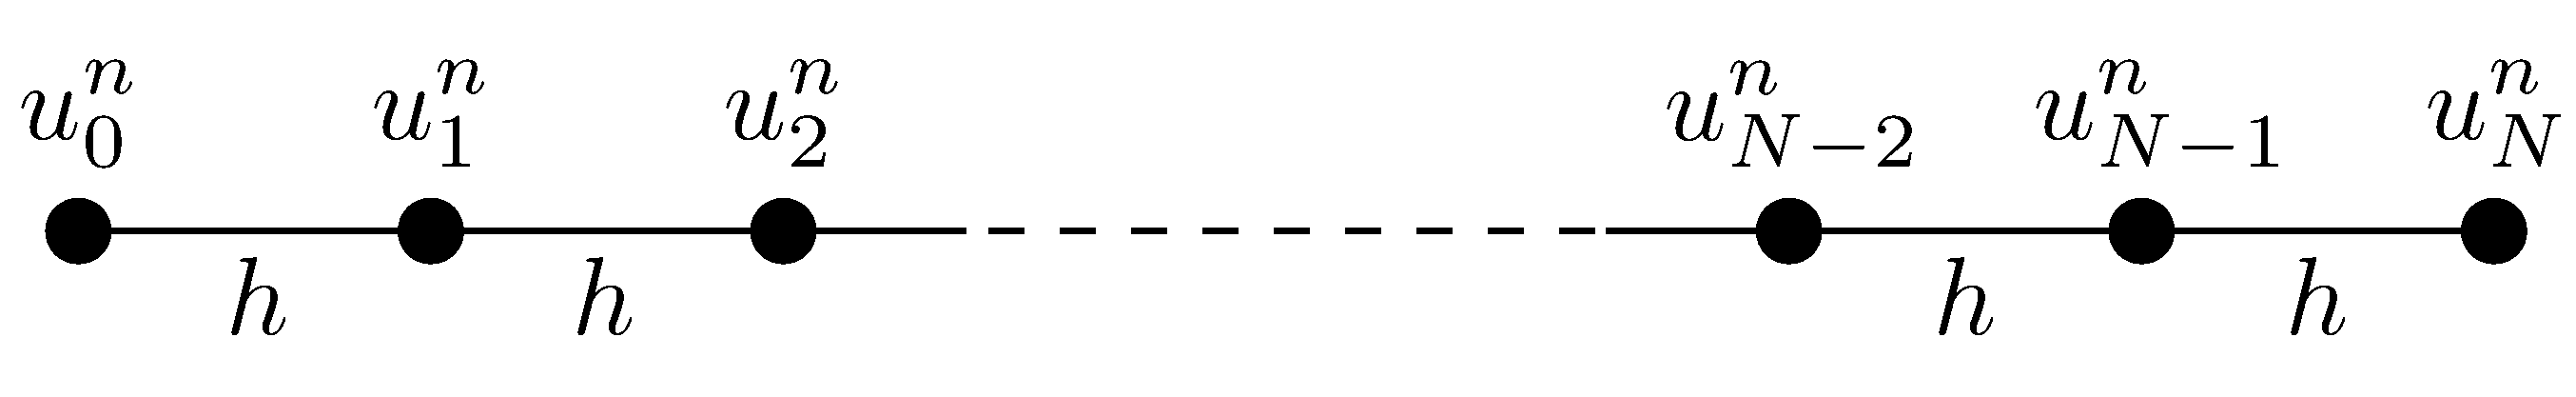
\includegraphics[width=0.45\textwidth]{figures/fdtd/gridExplanation.pdf}}\hspace{0.06\textwidth}
    % \subfloat[If $N$ is large (as is usually the case), The 1D system is divided into $N$ sections of length $h$ and $l=\{0, \hdots, N\}$.\label{fig:gridExp2}]{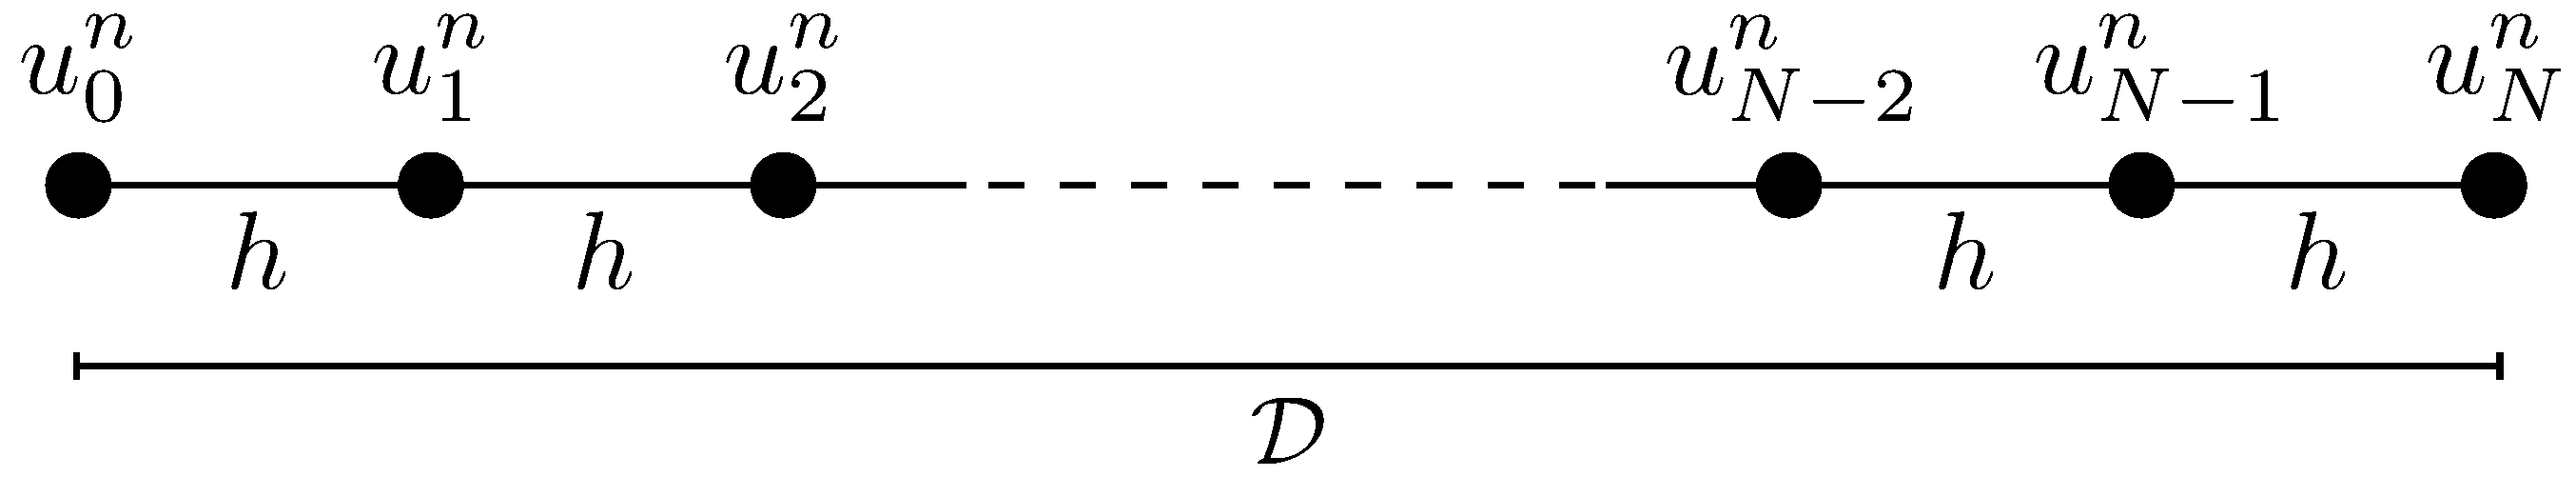
\includegraphics[width=0.45\textwidth]{figures/fdtd/gridExplanation2.pdf}}
    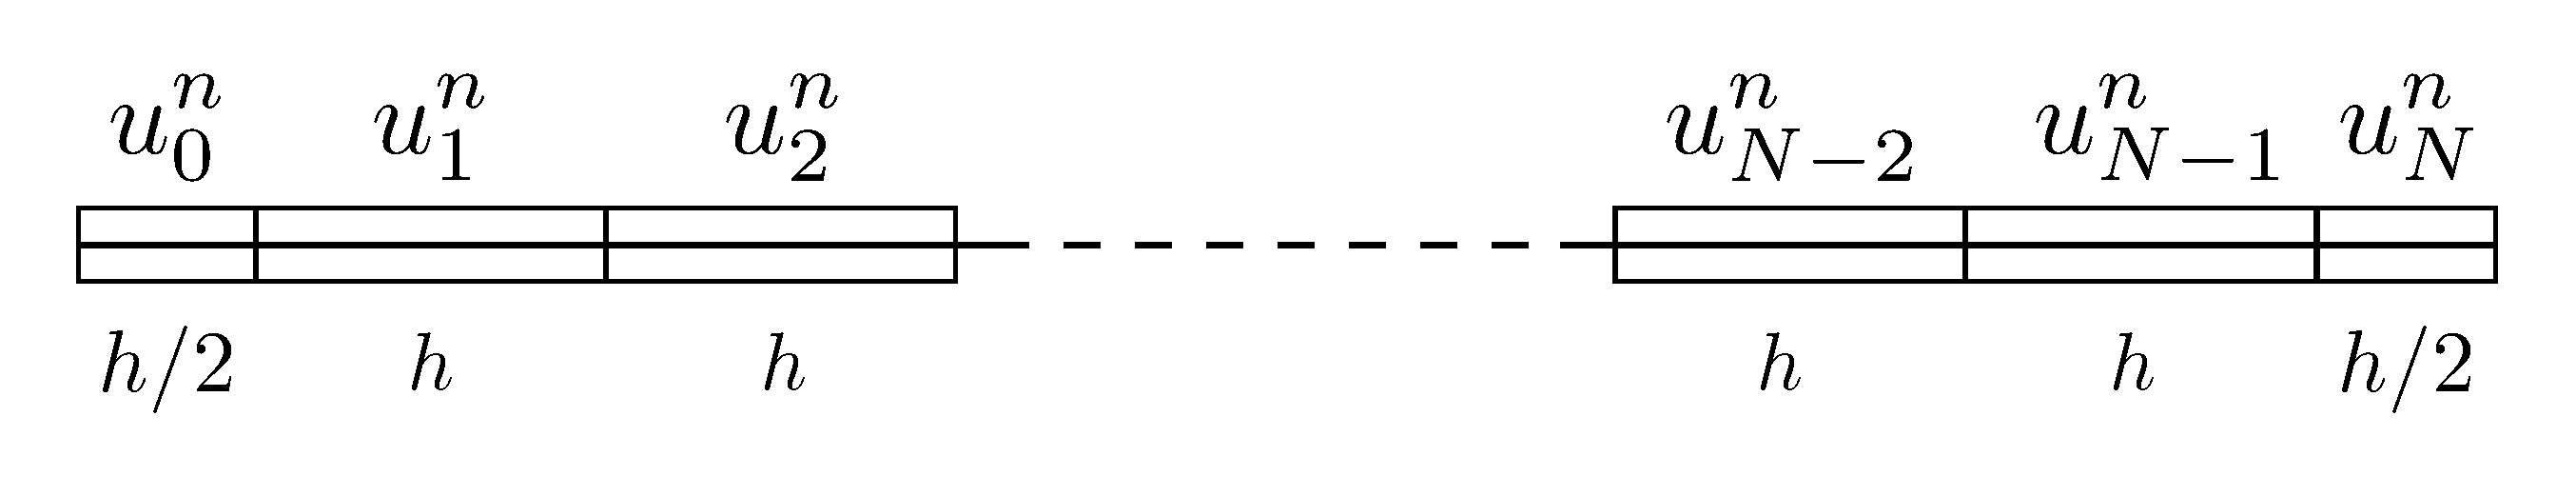
\includegraphics[width=0.75\textwidth]{figures/fdtd/gridFigure2.pdf}
    \caption{Alternative interpretation of the discretisation of $u(x,t)$. The continuous system is divided into $N-1$ sections of width $h$ plus $2$ sections of width $h/2$ at the boundaries. Through this interpretation, the `weight' of a grid point can be calculated from its physical parameters. \label{fig:gridExp2}}
\end{figure}

\section{Connected ideal strings}\label{sec:connIdealStrings}
As an test case for the following sections, consider two ideal strings of length $L_u$ and $L_w$ (both in m) their transverse displacement denoted as $u=u(x,t)$ and $w = w(\chi,t)$ (both in m) (see Section \ref{sec:1DWave}).\footnote{Recall that the ideal string is the 1D wave equation with $c=\sqrt{T/\rho A}$.}  The systems are defined for $x\in \D_u$ with domain $\D_u=[0,L_u]$ and $\chi \in \D_w$ with domain $\D_w=[0,L_w]$ respectively. Notice that $\chi$ is used as the spatial coordinate for $w$ to denote that the two systems use different coordinate systems. Connecting these systems at $x_\ctxt\in \D_u$ and $\chi_\ctxt\in\D_w$ yields the following system of PDEs:
\begin{subequations}\label{eq:conn1DwavePDE}
    \begin{align}
        \rho_u A_u \ptt u &= T_u \pxx u -\delta(x-x_\ctxt)f, \label{eq:conn1DwavePDEu} \\
        \rho_w A_w \ptt w &= T_w \partial_\chi^2 w + \delta(\chi-\chi_\ctxt)f,\label{eq:conn1DwavePDEw}
    \end{align}
\end{subequations}
where subscripts $u$ and $w$ denote whether a variable belongs to system $u$ or $w$ respectively. Notice that the $\partial_\chi$ in Eq. \eqref{eq:conn1DwavePDEw} denotes a partial derivative with respect to $\chi$ and is an identical operation to $\px$, but on a different coordinate system. Furthermore, $f = f(t)$ is the connection force (in N) which should be equal and opposite for the connected systems (hence the inverse signs). The definition for $f$ depends on the connection type, and two alternatives will be given shortly. Finally, the spatial Dirac delta function $\delta$ is defined as in Eq. \eqref{eq:spatialDirac}, and localises the connection force along the systems. 
% The relative displacement between the two systems at their respective connection locations (in m) is defined as 
% \begin{equation}
%     \eta(t) = u(x_\text{c},t) - w_(\chi_\ctxt),
% \end{equation}
% and will be used later on. 

\subsubsection{Relative location of objects}\todo{COLLISION CONNECTION}
When working with multiple interacting objects, it is important to keep in mind relative location of the connected objects, i.e., whether one object is `above' or `below' an other. This relative location will affect sign of the force term. As a connection should `pull' the systems towards each other, the connection force should have a negative effect on the object `above' and a positive effect on the object `below'. From the signs of the force terms in system \eqref{eq:conn1DwaveFDS}, one can observe that $u$ has been placed above $w$.  

\subsection{Discrete time}
One can then discretise the state variables $u$ and $w$ to grid functions $\uln$ and $\wmn$ using $x = lh_u$ and $\chi = mh_w$ where $l\in \{0, \hdots, N_u\}$ and $m\in \{0, \hdots, N_w\}$.\footnote{Here, $m$ is used for the spatial index of $\wmn$ to avoid double subscripts $l_u$ and $l_w$.} Also see Section \ref{sec:gridFunctions}. Furthermore, $h_u$ and $h_w$ are the values of the grid spacing (both in m) and $N_u+1$ and $N_w+1$ are the number of grid points for $\uln$ and $\wmn$ respectively. Dividing Eqs. \eqref{eq:conn1DwavePDEu} and \eqref{eq:conn1DwavePDEw} by $\rho_u A_u$ and $\rho_w A_w$ respectively yields
\begin{subequations}\label{eq:conn1DwaveFDS}
    \begin{align}
        \dtt \uln &= c_u^2 \dxx \uln -\Ju\frac{f^n}{\rho_u A_u}, \label{eq:conn1DwaveFDSu} \\
        \dtt \wmn &= c_w^2 \delta_{\chi\chi} \wmn + \Jw\frac{f^n}{\rho_w A_w},\label{eq:conn1DwaveFDSw}
    \end{align}
\end{subequations}
where $c_u = \sqrt{T_u / \rho_uA_u}$ and $c_w = \sqrt{T_w / \rho_wA_w}$. The spreading operators $\Ju = J_{l, o_u, u}(x_\ctxt)$ and $J_{l, w}(\chi_\ctxt) = J_{l, o_w, w}(\chi_\ctxt)$ are as defined in Section \ref{sec:interpolationSpreading}, and their orders $o_u$ and $o_w$ are left unspecified. 

The next step would be to solve for connection force $f^n$. First, one needs to isolate the schemes in system \eqref{eq:conn1DwaveFDS} at their respective connection locations $x_\ctxt$ and $\chi_\ctxt$. This is done by taking an inner product of each scheme in system \eqref{eq:conn1DwaveFDS} with their respective spreading operator $J_{l, u}$ and $J_{l, w}$ over discrete domains $d_u = \{0, \hdots, N_u\}$ and $d_w = \{0, \hdots, N_w\}$ respectively. Using identity \eqref{eq:identityIJ} one can write
\begin{subequations}\label{eq:conn1DwaveFDSXc}
    \begin{align}
        \Iu\dtt \uln &= c_u^2 \Iu\dxx \uln -\lVert \Ju\rVert_{d_u}^2\frac{f^n}{\rho_u A_u}, \label{eq:conn1DwaveuXc} \\
        \Iw\dtt \wmn &= c_w^2 \Iw\delta_{\chi\chi} \wmn + \lVert \Jw\rVert_{d_w}^2\frac{f^n}{\rho_w A_w},\label{eq:conn1DwavewXc}
    \end{align}
\end{subequations}
Here, interpolation operators $\Iu = I_{l, o_u, u}(x_\ctxt)$ and $\Iw = I_{l, o_w, w}(\chi_\ctxt)$ are as defined in Section \ref{sec:interpolationSpreading}. Notice that the order of these operators need 
to match their `dual' spreading operator, but the orders $o_u$ and $o_w$ may differ.

The definition of the force depends on the connection type. Below, two alternatives will be presented: the rigid connection and the spring connection. 

\section{Rigid connection}\label{sec:rigidConn}
The simplest connection-type is the \textit{rigid connection}. This connection type states that the displacement of two connected points should always be equal, and thus the distance between them should be 0 at all times. 
For the rigid connection, the following is true
\begin{equation}\label{eq:contRigid}
    u(x_\ctxt, t) = w(\chi_\ctxt, t),
\end{equation}
which in discrete time becomes
\begin{equation}\label{eq:discRigid}
    \Iu\uln = \Iw\wmn.
\end{equation}
If Eq. \eqref{eq:discRigid} is true, the following must also hold:
\begin{equation}\label{eq:discAccelRigid}
    \Iu\dtt\uln = \Iw\dtt\wmn.
\end{equation}
In other words, if the displacement of two objects is equal, their acceleration must also be. This definition can then immediately be used to solve for $f^n$ and the right-hand sides in system \eqref{eq:conn1DwaveFDSXc} can be substituted in Eq. \eqref{eq:discAccelRigid} to get
\begin{equation*}
    c_u^2 \Iu\dxx \uln -\lVert \Ju\rVert_{d_u}^2\frac{f^n}{\rho_u A_u}
    \!=\! c_w^2 \Iw\delta_{\chi\chi} \wmn + \lVert \Jw\rVert_{d_w}^2\frac{f^n}{\rho_w A_w},
\end{equation*}
which can be explicitly solved for $f^n$ according to
\begin{equation}\label{eq:rigidForce}
    f^n = \frac{c_u^2 \Iu\dxx \uln - c_w^2 \Iw\delta_{\chi\chi} \wmn}{\frac{\lVert \Ju\rVert_{d_u}^2}{\rho_u A_u} + \frac{\lVert \Jw\rVert_{d_w}^2}{\rho_w A_w}}.
\end{equation}
This value can then be used in the update equation obtained after expanding system \eqref{eq:conn1DwaveFDS} as
\begin{subequations}
    \begin{align}
        \!\!\!u_l^{n+1} &= \left(2-2\lambda_u^2\right) \uln  + \lambda_u^2\left(u_{l+1}^n + u_{l-1}^n\right) - u_l^{n-1} -\Ju\frac{k^2 f^n}{\rho_u A_u}\\
        \!\!\!w_m^{n+1} &= \left(2-2\lambda_w^2\right) \wmn\! +\! \lambda_w^2\left(w_{m+1}^n\! +\! w_{m-1}^n\right) \! -\! w_m^{n-1} +\Jw\frac{k^2 f^n}{\rho_w A_w}
    \end{align}
\end{subequations}
where $\lambda_u = c_uk/h_u \leq 1$ and  $\lambda_u = c_uk/h_u \leq 1$ are the Courant numbers for each individual scheme (see Section \ref{sec:1DWave}).

Figure \ref{fig:connectedWaveEqs} shows an implementation of system \eqref{eq:conn1DwaveFDS} with $x_\ctxt = 0.25$ m and $\chi_\ctxt = 0.75$ m. The wave equations have the same mass per unit length, i.e., $\rho_uA_u = \rho_wA_w$, and the same length $L_u=L_w = 1$ m, but operate at different wave speeds $c_u=300$ m/s and $c_w=400$ m/s.

\begin{figure}[h]
    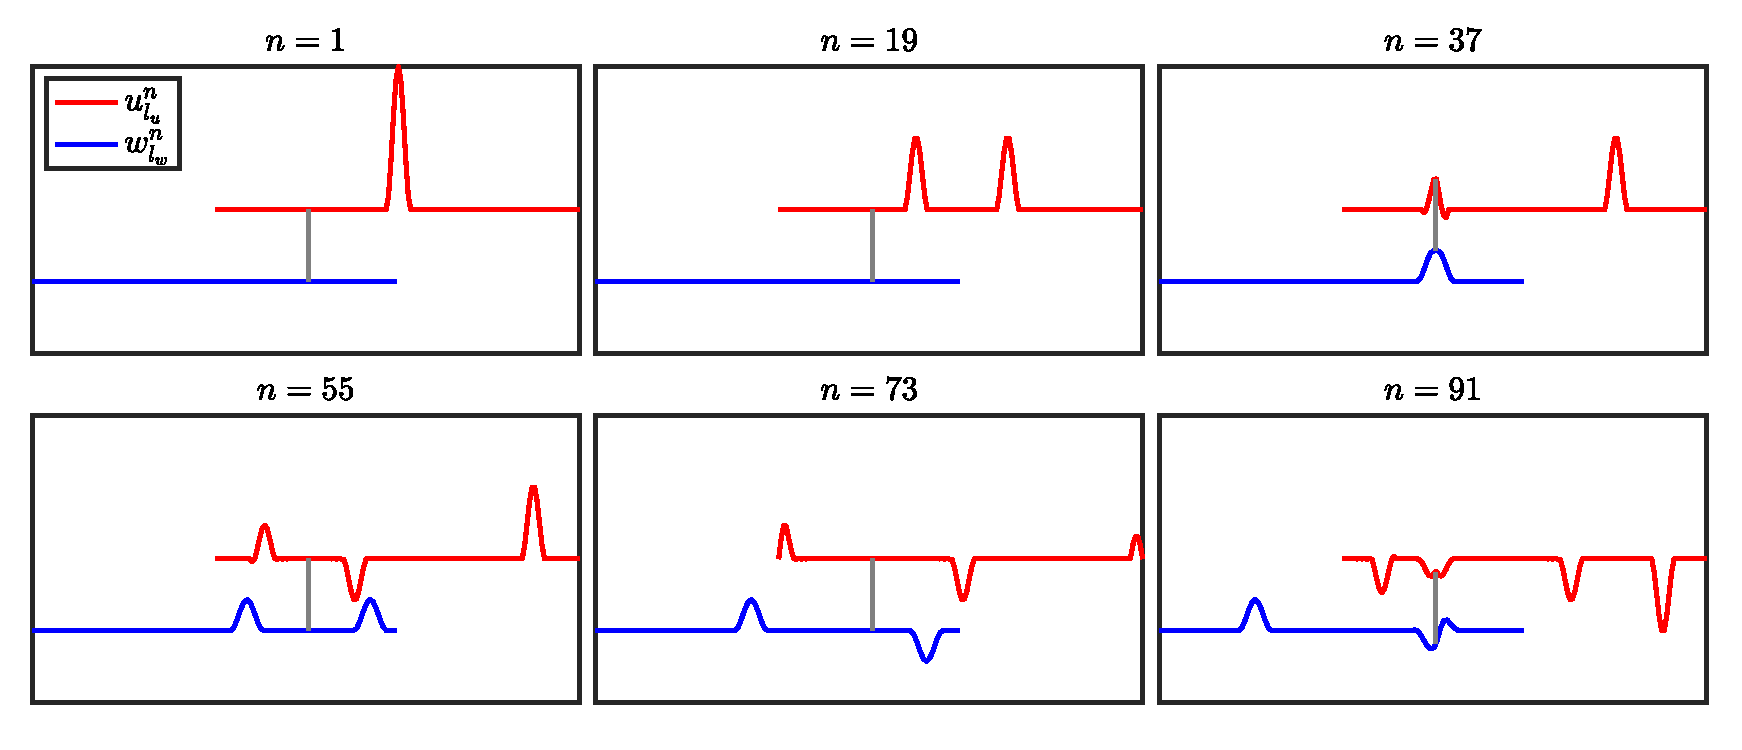
\includegraphics[width=\textwidth]{figures/interactions/connectedWaveEqs.eps}
    \caption{The wave propagation of two connected 1D wave equations with the same mass per unit length. The systems are offset for clarity, but the relative displacement at the connection location is 0. \label{fig:connectedWaveEqs}}
\end{figure}

\subsubsection{Notation simplification}
In the above equations, the orders of the spreading and interpolation operators have been left unspecified to retain generality. If one would like to connect two systems at specified grid points without needing to worry about interpolation, the notation can greatly simplified.%\footnote{The same can be achieved if the orders of the interpolation and spreading operators are chosen to be 0, or if $\alpha_\itxt = 0$ for arbitrary orders.}

Recalling that $\Iu = I_{l, o_u, u}(x_\ctxt)$ and $\Iw = I_{l, o_w, w}(\chi_\ctxt)$, one can set the interpolation orders to 0, i.e., $o_u = o_w = 0$, to yield the following short-hand notations
\begin{equation}\label{eq:shorthandI}
    I_{l,0,u}(x_\text{c})\uln = \ulcn, \qaq I_{m,0,w}(\chi_\text{c})\wmn = \wmcn,
\end{equation}
where $l_\ctxt = \floor[x_\ctxt/h_u]$ and $m_\ctxt = \floor[\chi_\ctxt/h_w]$, and
\begin{equation}\label{eq:shorthandJ}
    \lVert J_{l, 0, u}(x_\text{c})\rVert_{d_u}^2 = \frac{1}{h_u}, \qaq \lVert J_{m, 0, w}(\chi_\text{c})\rVert_{d_w}^2 = \frac{1}{h_w}.
\end{equation}
This simplifies Eqs. \eqref{eq:conn1DwaveFDSXc} to
\begin{subequations}\label{eq:conn1DwaveFDSXcSimple}
    \begin{align}
        \dtt \ulcn &= c_u^2 \dxx \ulcn -\frac{f^n}{\rho_u A_u h_u}, \label{eq:conn1DwaveuXcSimple} \\
        \dtt \wmcn &= c_w^2 \delta_{\chi\chi} \wmcn + \frac{f^n}{\rho_w A_w h_w},\label{eq:conn1DwavewXcSimple}
    \end{align}
\end{subequations}
which, after rewriting Eq. \eqref{eq:discAccelRigid} to
\begin{equation}
    \dtt\ulcn = \dtt\wmcn,
\end{equation}
one can solve for $f^n$, yielding the following  simplified form of Eq. \eqref{eq:rigidForce}
\begin{equation}
    f^n = \frac{c_u^2 \dxx \ulcn - c_w^2 \delta_{\chi\chi} \wmcn}{\frac{1}{\rho_u A_u h_u} + \frac{1}{\rho_w A_w h_w}}.
\end{equation}

\subsection{Energy Analysis}\label{sec:energyAnalysis1DwaveConnRigid}
This section follows the energy analysis techniques shown in Section \ref{sec:energyAnalysis} (though not explicitly following Steps 1-4). As the analysis has previously been performed on the 1D wave equation, this part of the analysis will not be detailed here. 

Starting with the FD scheme in Eq. \eqref{eq:conn1DwaveFDSu}, one can take an inner product of the scheme (after a multiplication with $\rho_u A_u$) with $(\dtd\uln)$ over discrete domain $d_u$ to get
\begin{equation}\label{eq:powerBalanceConn1DwaveU}
    \dtp \h_u = \langle \dtd\uln, -\Ju f^n\rangle_{d_u},
\end{equation}
where $\h_u$ is the total energy in system $u$ and is as defined in Eq. \eqref{eq:energyBalance1DWave}. The same can be done for Eq. \eqref{eq:conn1DwaveFDSw} (after a multiplication with $\rho_w A_w$) by taking an inner product with $(\dtd\wmn)$ over discrete domain $d_w$ ti get 
\begin{equation}\label{eq:powerBalanceConn1DwaveW}
    \dtp \h_w = \langle \dtd\wmn, \Jw f^n\rangle_{d_w},
\end{equation}
where $\h_w$ is the total energy in system $w$. As the total energy in the system is an addition of $\h_u$ and $\h_w$, and using identity \eqref{eq:identityIJ} for the the right hand sides of Eqs. \eqref{eq:powerBalanceConn1DwaveU} and \eqref{eq:powerBalanceConn1DwaveW}, one can write 
\begin{equation}\label{eq:rOCconnSystem}
    \dtp (\h_u + \h_w) = -\Iu \dtd \uln f^n + \Iw \dtd \wmn f^n.
\end{equation}
Finally, due to the rigid connection in Eq. \eqref{eq:discRigid}, $\Iu \dtd \uln = \Iw \dtd \wmn$ (if the displacements are equal, their velocities must also be) and the right hand side vanishes:
\begin{equation*}
    \dtp (\h_u + \h_w) = 0.
\end{equation*}
This shows that the rigid connection does not affect the total energy in the system and thus does not affect the stability of the scheme.

Figure \ref{fig:energyConn1DWave} shows the energy of an implementation of the 1D wave system in \eqref{eq:conn1DwaveFDS}. The 
\begin{figure}[h]
    \centering
    \begin{tikzpicture}[->,node distance=3cm,
        thick,main node/.style={circle,draw}]
    
        \node[] (image) at (0,0) {
        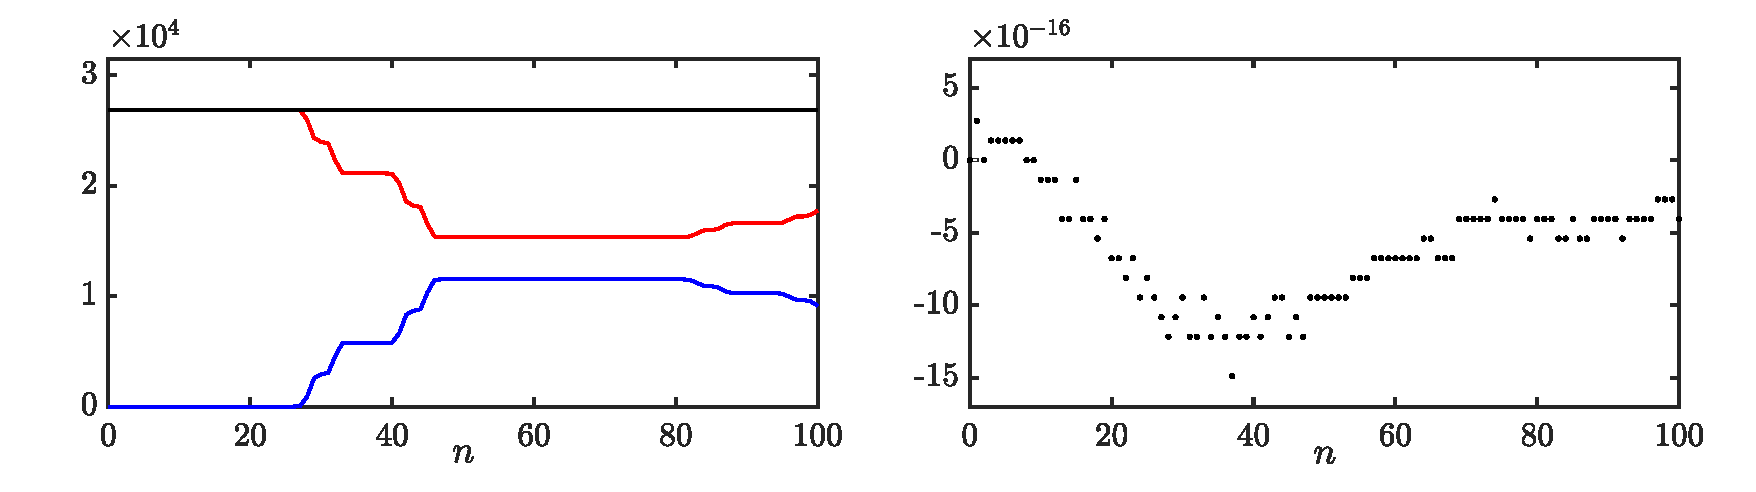
\includegraphics[width=\textwidth]{figures/interactions/connected1DEnergy.eps}
        };
    
        \node[] (he) at (0.2,0.5) {\small $\mathfrak{h}_\text{e}$};

        \node[] (h) at (-5.8, 1) {\small $\mathfrak{h}$};
        \node[] (v) at (-5.8, 0.5) {\small $\color{red}\mathfrak{h}_u$};
        \node[] (t) at (-5.8, 0) {\small $\color{blue}\mathfrak{h}_w$};
      \end{tikzpicture}
      \caption{The energy of $u$ (blue), the energy of $w$ (red), and the total (black) energy of the system of connected 1D wave equations in \eqref{eq:conn1DwaveFDS}. The energy corresponds to Figure \ref{fig:connectedWaveEqs}. The right panel shows the normalised energy (according to Eq. \eqref{eq:normalisedEnergy} shows that the deviation of the energy is within machine precision. \label{fig:energyConn1DWave}}
\end{figure}

\subsection{Matrix form}\label{sec:matrixFormRigid}
% In order to perform a modal analysis on the system, one must use the matrix form of the system in Eq. \eqref{eq:conn1DwaveMatrix}. 

One can write the system in Eq. \eqref{eq:conn1DwaveFDS} with a rigid connection in matrix form, albeit slightly more involved due to the interconnection of the schemes.

To start, the definition of the force in Eq. \eqref{eq:rigidForce} must be substituted into the system, which, after expansion of the left hand side of the system, becomes
\begin{subequations}\label{eq:forceExpanded1Dwaves}
    \begin{align}
        &\begin{aligned}
            u_l^{n+1} &= 2\uln - u_l^{n-1} + c^2k^2\dxx \uln \\
            &- \Ju\frac{k^2}{\rho_u A_u} \left(\frac{c_u^2 \Iu\dxx \uln - c_w^2 \Iw\delta_{\chi\chi} \wmn}{\frac{\lVert \Ju\rVert_{d_u}^2}{\rho_u A_u} + \frac{\lVert \Jw\rVert_{d_w}^2}{\rho_w A_w}}\right), 
        \end{aligned}\\
        &\begin{aligned}
            w_m^{n+1} &= 2\wmn - w_m^{n-1} + c^2k^2\dxx \wmn \\
            &+ \Jw\frac{k^2}{\rho_w A_w} \left(\frac{c_u^2 \Iu\dxx \uln - c_w^2 \Iw\delta_{\chi\chi} \wmn}{\frac{\lVert \Ju\rVert_{d_u}^2}{\rho_u A_u} + \frac{\lVert \Jw\rVert_{d_w}^2}{\rho_w A_w}}\right).
        \end{aligned}
    \end{align}
\end{subequations}
Using Dirichlet boundary conditions for both ideal strings, their values can be stored in the following vectors
\begin{equation*}
    \u^n =[u_1^n, \hdots, u_{N_u-1}^n]^T, \qaq \w^n =[w_1^n, \hdots, w_{N_u-1}^n]^T.
\end{equation*}
These vectors can then be concatenated to one larger state vector and after the terms in Eqs. \eqref{eq:forceExpanded1Dwaves} are grouped by the grid functions at various time indices, one obtains the following compact matrix form of system \eqref{eq:conn1DwaveFDS}:
\begin{equation}\label{eq:conn1DwaveMatrix} 
    \begin{bmatrix}
        \u^{n+1}\\
        \w^{n+1}
    \end{bmatrix} = \B \begin{bmatrix}
        \u^n\\
        \w^n
    \end{bmatrix} - \begin{bmatrix}
        \u^{n-1}\\
        \w^{n-1}
    \end{bmatrix}
\end{equation}
% \begin{equation}
%     \mathbf{v}^{n+1} = \B \mathbf{v}^n - \mathbf{v}^{n-1}
% \end{equation}
where 
\begin{equation*}
    \B = \begin{bmatrix}
        \B_u & \mathbf{0}\\
        \mathbf{0} & \B_w 
    \end{bmatrix} + \begin{bmatrix}
        -\j_u\\
        \j_w
    \end{bmatrix}
    \begin{bmatrix}
        \mathbf{f}_u& -\mathbf{f}_w
    \end{bmatrix}.
\end{equation*}
The first matrix in the definition of $\B$ contains the operations of the 1D wave equation (also see Eq. \eqref{eq:1DwaveMatrix}),
\begin{equation}    
    \B_u = 2\I_{N_u-1} +c_u^2k^2 (\Dxx)_u \qaq \B_w = 2\I_{N_w-1} +c_w^2k^2 (\Dxx)_w
\end{equation}
where matrices $(\Dxx)_u$ and $(\Dxx)_w$ are as defined in Eq. \eqref{eq:DxxDef} and are of the appropriate sizes. The vector multiplication in the definition of $\B$ results in a matrix, and adds the effect of the connection force to the system. Here, $\j_u$ and $\j_w$ are column vectors of size $(N_u-1)\times 1$ and $(N_w-1)\times 1$ containing the values of the spreading operators $\Ju$ and $\Jw$ respectively. Finally,
\begin{align*}
    \mathbf{f}_u = \frac{k^2}{\rho_uA_u} \left(\frac{c_u^2\i_u(\Dxx)_u}{\frac{\i_u \j_u}{ \rho_u A_u} + \frac{\i_w \j_w}{\rho_w A_w}}\right),& \quad \mathbf{f}_w =  \frac{k^2}{\rho_uA_u}\left(\frac{c_w^2k^2 \i_w(\Dxx)_w}{\frac{\i_u \j_u}{ \rho_u A_u} + \frac{\i_w \j_w}{\rho_w A_w}}\right),
\end{align*}
%are row vectors of size $1\times (N_u-1)$ and $1\times (N_w-1)$, 
where $\i_u$ and $\i_w$ are row vectors of size $1\times (N_u-1)$ and $1\times (N_w-1)$ containing the values of the interpolation operators $\Iu$ and $\Iw$ respectively. Finally, $\i_u\j_u$ and $\i_w\j_w$ are matrix-vector forms of $\lVert \Ju\rVert_d^2$ and $\lVert \Jw\rVert_d^2$ respectively (see Eq. \eqref{eq:JnormIJ}) and reduce to a scalar. \SWcomment[check with stefan if this is a correct notation for this]

Equation \eqref{eq:conn1DwaveMatrix} can then easily be rewritten in one-step form as described in Section \ref{sec:oneStepForm} and used for modal analysis.\footnote{Due to the lack of damping in the system, the system could be analysed directly, not using a one-step form.}
% Following Section \ref{sec:oneStepForm}, one can rewrite Eq. \eqref{eq:conn1DwaveMatrix} to

% \begin{equation}
%     \underbrace{\begin{bmatrix}
%         \u^{n+1}\\
%         \w^{n+1}\\
%         \u^{n}\\
%         \w^{n}
%     \end{bmatrix}}_{\mathbf{v}^{n+1}} = \underbrace{\begin{bmatrix}
%         \B & -\I\\
%         \I,& \mathbf{0}
%     \end{bmatrix}}_{\Q}\underbrace{\begin{bmatrix}
%         \u^{n}\\
%         \w^{n}\\
%         \u^{n-1}\\
%         \w^{n-1}
%     \end{bmatrix}}_{\mathbf{v}^n},
% \end{equation}
% one can insert a test solution $\mathbf{v}^n=z^n\boldPhi$ to get
% \begin{equation*}
%     z\boldPhi = \Q\boldPhi,
% \end{equation*}
% and solved for the $p$\th eigenvalue by following the process in Section \ref{sec:oneStepForm}.

% \todo{figure?}

\section{Spring connection}\label{sec:springConnection}
An alternative connection type is the \textit{spring connection}. As in the rigid case, forces are still equal and opposite, but spring connections allow the relative displacement between the two connected elements to be non-zero. This relative displacement is used to determine the connection force. Interestingly, nonlinearities can be added in a fairly straightforward manner, after which the system can still be solved explicitly.\todo{wording} The most complex springs used in this project have a linear and a nonlinear component, as well as a damping term. For ease of explanation, this section will only use a linear spring. A damped nonlinear spring will appear in Section \ref{sec:stringPlateConnection}. 

The force between two components connected by a linear spring can be defined as
\begin{equation}\label{eq:linearSpringForceCont}
    f = f(t) = K\eta,
\end{equation}
where $K\geq 0$ is the spring constant (in N/m) and
\begin{equation}\label{eq:etaLinSpringCont}
    \eta = \eta(t) = u(x_\ctxt, t) - w(\chi_\ctxt, t)
\end{equation}
is the relative displacement between the two systems at their respective connection locations (in m).\footnote{Note that if $u$ was placed 'below' $w$ (see Section \ref{sec:connIdealStrings}), the signs of the force terms in system \eqref{eq:conn1DwaveFDS} would have been flipped and $u(x_\ctxt, t)$ would have been subtracted from $w(\chi_\ctxt, t)$ in Eq. \eqref{eq:etaLinSpringCont} instead.} 

% This is important for the signs when adding the force terms to the schemes.
%$\eta$ is thus also, effectively, the length of the spring.

In discrete time, Eq. \eqref{eq:linearSpringForceCont} becomes
\begin{equation}\label{eq:linearSpringForceDisc}
    f^n = K\mtd\eta^n,
\end{equation}
where
\begin{equation}\label{eq:discEtaConn1Dwave}
    \eta^n = \Iu\uln - \Iw\wmn.
\end{equation}
Here, the centred averaging operator is used for stability (see Section \ref{sec:conn1DwaveEnergySpring}), but when substituted into Eq. \eqref{eq:conn1DwaveFDSXc} seems to make the system implicit. However, one can find an explicit solution, even for an arbitrary amount of connections \cite{Bilbao2009Modular}. These systems are therefore referred to as being \textit{semi-implicit}, and an explicit solution will be shown below.

\subsection{Explicit solution}\label{sec:explicitSolutionSpringConn}
When compared to the rigid connection in Section \ref{sec:rigidConn}, solving for $f^n$ requires an extra step. After isolating the schemes at their respective connection locations -- resulting in Eqs. \eqref{eq:conn1DwaveFDSXc} -- one needs to expand the scheme and solve for the states at $n+1$:
\begin{subequations}\label{eq:intermediateConn1Dwave}
    \begin{align}
        \Iu u_l^{n+1} &= u^\star - \lVert\Ju\rVert_{d_u}^2 \frac{k^2f^n}{\rho_u A_u},\\
        \Iw w_m^{n+1} &= w^\star + \lVert\Jw\rVert_{d_w}^2 \frac{k^2f^n}{\rho_w A_w},
    \end{align}
\end{subequations}
where
\begin{equation*}
    u^\star = \Iu(2\uln - u_l^{n-1}) + c_u^2k^2\Iu\dxx\uln,
\end{equation*}
and
\begin{equation*}
    w^\star = \Iw(2\wmn - w_m^{n-1}) + c_w^2k^2\Iw\dxx\wmn,
\end{equation*}
are the update equations of the system at their respective connection locations without the term containing the connection force\todo{COLLISION CONNECTION (refer to Collision chapter if this is chapter 11 now}. Evaluating Eq. \eqref{eq:discEtaConn1Dwave} at $n+1$ yields
\begin{equation*}
    \eta^{n+1} = \Iu u_l^{n+1} - \Iw w_m^{n+1},
\end{equation*}
into which Eqs. \eqref{eq:intermediateConn1Dwave} can be substituted
\begin{equation}\label{eq:etaNp1Schemes}
    \eta^{n+1} = u^\star - \lVert\Ju\rVert_{d_u}^2 \frac{k^2f^n}{\rho_u A_u} - \left(w^\star + \lVert\Jw\rVert_{d_w}^2 \frac{k^2f^n}{\rho_w A_w}\right).
\end{equation}
A second definition for $\eta^{n+1}$ can be obtained after expanding Eq. \eqref{eq:linearSpringForceDisc}:
\begin{equation}\label{eq:etaExpanded}
    \eta^{n+1} = \frac{2 f^n}{K} - \eta^{n-1}
\end{equation}
and can be substituted into Eq. \eqref{eq:etaNp1Schemes} to get
\begin{equation}
    \frac{2 f^n}{K} - \eta^{n-1} = u^\star - \lVert\Ju\rVert_{d_u}^2 \frac{k^2f^n}{\rho_u A_u} - \left(w^\star + \lVert\Jw\rVert_{d_w}^2 \frac{k^2f^n}{\rho_w A_w}\right).
\end{equation}
Finally, one can group the terms for $f^n$ 
\begin{equation*}
    \left(\frac{2}{K} + \frac{\lVert\Ju\rVert_{d_u}^2k^2}{\rho_u A_u} +  \frac{\lVert\Jw\rVert_{d_w}^2k^2}{\rho_w A_w}\right)f^n = u^\star - w^\star + \eta^{n-1}
\end{equation*}
and solve for the force, solely based on known values of the system
\begin{equation}
    f^n = \frac{u^\star - w^\star + \eta^{n-1}}{\frac{2}{K} + \frac{\lVert\Ju\rVert_{d_u}^2k^2}{\rho_u A_u} +  \frac{\lVert\Jw\rVert_{d_w}^2k^2}{\rho_w A_w}}\ .
\end{equation}

Figure \ref{fig:connectedWaveEqsSpring} shows the wave propagation of the system connected with a spring with spring constant $K = 5\cdot 10^4$ N/m. The same parameters and excitation are used as for the rigid connection in Section \ref{sec:rigidConn}. When compared to the wave propagation of the system with a rigid connection in Figure \ref{fig:connectedWaveEqs}, one can observe that, the transfer of energy from $u$ to $w$ is slower than in the rigid case due to the extension of the spring.

\begin{figure}[h]
    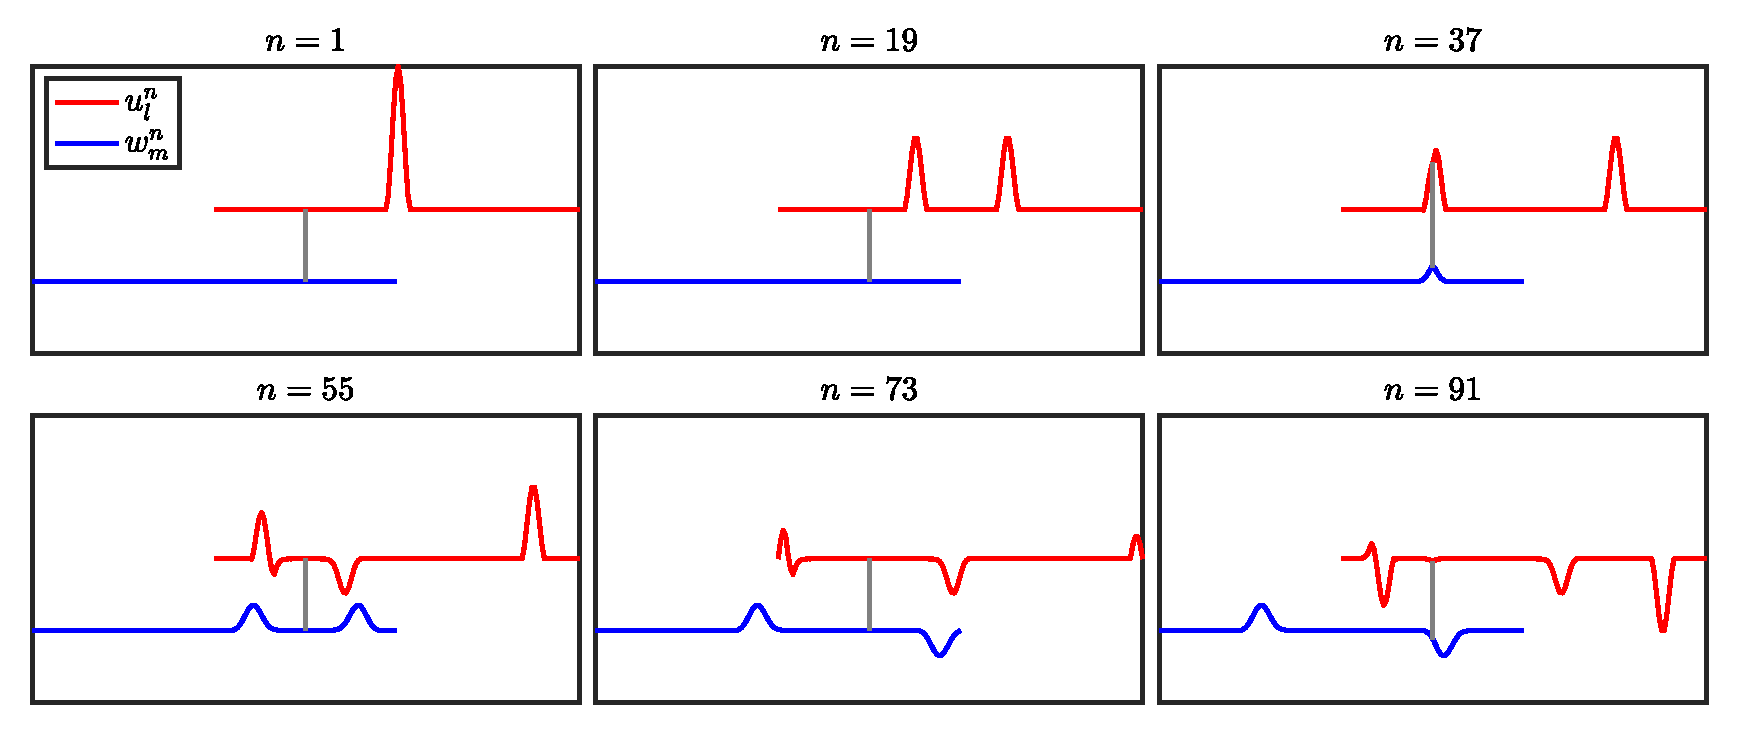
\includegraphics[width=\textwidth]{figures/interactions/connectedWaveEqsSpring.eps}
    \caption{The wave propagation of two ideal strings with the same mass per unit length connected using a spring with $K = 5 \cdot 10^4$ N/m. \label{fig:connectedWaveEqsSpring}}
\end{figure}

\subsection{Energy analysis}\label{sec:conn1DwaveEnergySpring}
As springs store energy themselves, it needs to be shown that stability is maintained.\todo{wording} That the discretisation of the spring force chosen in Eq. \eqref{eq:linearSpringForceDisc} is inherently stable will be shown below. 

Following the same process as Section \ref{sec:energyAnalysis1DwaveConnRigid}, one can analyse system \eqref{eq:conn1DwaveFDS}, and arrive at Eq. \eqref{eq:rOCconnSystem}:
\begin{equation*}
    \dtp (\h_u + \h_w) = -\Iu \dtd \uln f^n + \Iw \dtd \wmn f^n,
\end{equation*}
which can be rewritten to
\begin{equation*}
    \dtp (\h_u + \h_w) = -\dtd\left(\Iu \uln - \Iw \wmn\right)f^n.
\end{equation*}
One can then substitute the definitions for $f^n$ and $\eta^n$ from Eqs. \eqref{eq:linearSpringForceDisc} and \eqref{eq:discEtaConn1Dwave} to get
\begin{equation}\label{eq:energyAfterForceSubstitution}
    \dtp (\h_u + \h_w) = -K(\dtd \eta^n) (\mtd \eta^n),
\end{equation}
which, using identity \eqref{eq:prodIdentity4}, can be rewritten to
\begin{equation}
    \dtp (\h_u + \h_w + \h_\ctxt) = 0,
\end{equation}
where
\begin{equation}
    \h_\ctxt = \frac{K}{2}\left(\mtm(\eta^n)^2\right)
\end{equation}
is the energy stored by the connection. As this definition is non-negative it is inherently stable. The spring stiffness $K$ could potentially be infinitely large, which would effectively reduce the spring connection to a rigid connection.

Figure \ref{fig:energyConn1DWaveSpring} shows the energy of an implementation of system \eqref{eq:conn1DwaveFDS} connected with a spring with stiffness $K=5\cdot 10^4$ and other parameters are the same as for the rigid connection in Section \ref{sec:rigidConn}. One can observe that when compared to the energetic behaviour of the system with a rigid connection in Figure \ref{fig:energyConn1DWave}, less energy is transferred from $u$ to $w$, and some energy is stored in the spring shown in green. 


\begin{figure}[h]
    \centering
    \begin{tikzpicture}[->,node distance=3cm,
        thick,main node/.style={circle,draw}]
    
        \node[] (image) at (0,0) {
        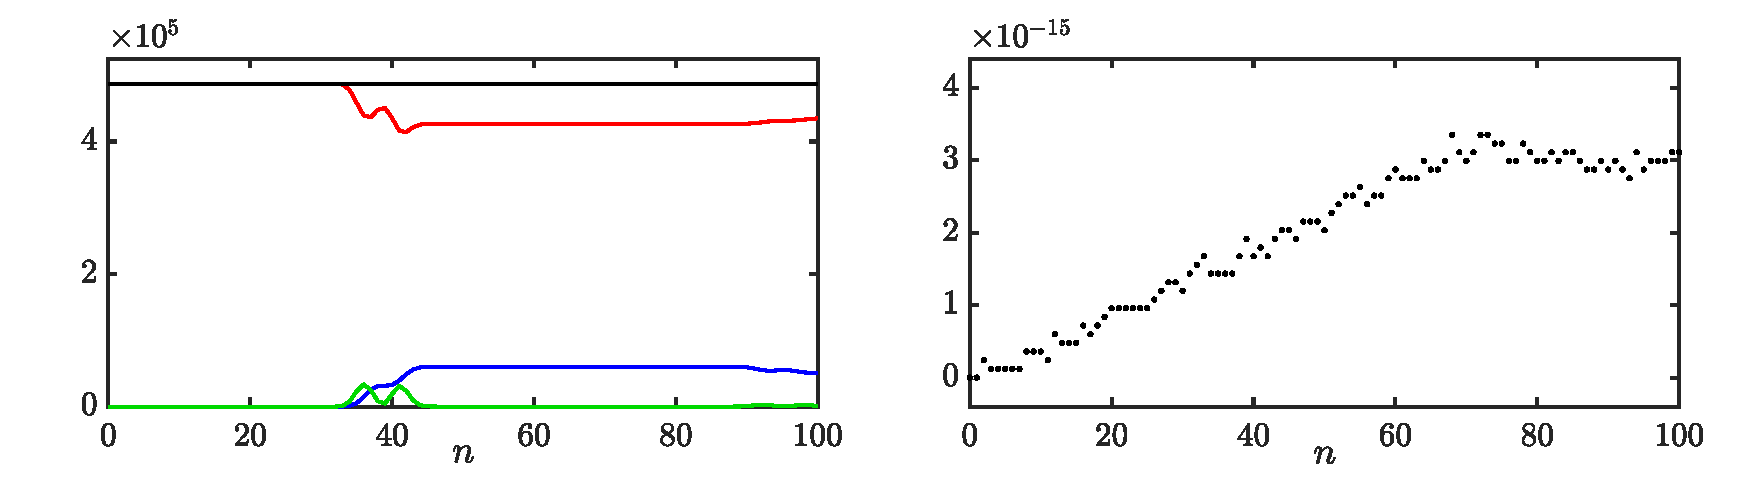
\includegraphics[width=\textwidth]{figures/interactions/connected1DEnergySpring.eps}
        };
    
        \node[] (he) at (0.2,0.5) {\small $\mathfrak{h}_\text{e}$};

        \node[] (h) at (-5.8, 1) {\small $\mathfrak{h}$};
        \node[] (v) at (-5.8, 0.5) {\small $\color{red}\mathfrak{h}_u$};
        \node[] (t) at (-5.8, 0) {\small $\color{blue}\mathfrak{h}_w$};
        \node[] (c) at (-5.8, -0.5) {\small $\color[HTML]{00DB00}\mathfrak{h}_\ctxt$};

      \end{tikzpicture}
      \caption{The energy of $u$ (blue), the energy of $w$ (red), the energy of the spring (green) and the total energy (black) of the system of connected 1D wave equations in \eqref{eq:conn1DwaveFDS}. The energy corresponds to the system in Figure \ref{fig:connectedWaveEqsSpring}. The right panel shows the normalised energy (according to Eq. \eqref{eq:normalisedEnergy}) shows that the deviation of the energy is within machine precision. \label{fig:energyConn1DWaveSpring}}
\end{figure}

\subsubsection{Unstable discretisation}
To show why an averaging operator is used in Eq. \eqref{eq:linearSpringForceDisc}, consider a more straightforward discretisation of Eq. \eqref{eq:linearSpringForceCont} without the averaging operator, such that
\begin{equation*}
    f^n = K\eta^n.
\end{equation*}
Performing an energy analysis of the system would yield 
\begin{equation*}
    \dtp (\h_u + \h_w) = -K(\dtd \eta^n) (\eta^n),
\end{equation*}
(instead of Eq. \eqref{eq:energyAfterForceSubstitution}) and using identity \eqref{eq:prodIdentity2}, this can be rewritten to
\begin{equation*}
    \dtp (\h_u + \h_w + \h_\ctxt) = 0,
\end{equation*}
where
\begin{equation*}
    \h_\ctxt = \frac{K}{2}\left(\eta^ne_{t-}\eta^n\right).
\end{equation*}
As this is not necessarily non-negative, the connection places a larger restriction on the stability of the system at the connection location. In other words, $\lambda \leq 1$ for the ideal strings does not ensure stability at the connection loaction. Also see \cite[pp. 190--192]{theBible}.

% \section{Spring-like connections}

% Forces are still equal and opposite as the springs are not distributed...

% \subsection{Connection with rigid barrier (scaled)}
% Consider the (scaled) 1D wave equation with an additional force term $F^n$
% \begin{equation}\label{eq:1DwaveConnRigid}
%     \dtt \uln = \gamma^2\dxx \uln + J_l(x_\ctxt)F^n
% \end{equation}
% where
% \begin{equation}\label{eq:1DwaveConnRigidForce}
%     F^n = -\omega_0^2\mtd\eta^n - \omega_1^4(\eta^n)^2\mtd\eta^n - 2\sigma_\times \dtd \eta^n
% \end{equation}
% and
% \begin{equation}\label{eq:etaRigid}
%     \eta^n = I_l(x_\ctxt)\uln.
% \end{equation}

% To obtain $F^n$, an inner product of scheme \eqref{eq:1DwaveConnRigid} needs to be taken with $J_l(x_\ctxt)$ over domain $\D$ which, using identity \eqref{eq:identityIJ} yields 
% \begin{equation}\label{eq:1DwaveConnRigidInnerProd}
%     \dtt I_l(x_\ctxt)\uln = \gamma^2 I_l(x_\ctxt)\dxx \uln + \underbrace{I_l(x_\ctxt)J_l(x_\ctxt)}_{\lVert J_l(x_\ctxt) \rVert^2_\D}F^n.
% \end{equation}
% As $u$ is connected to a rigid barrier according to \eqref{eq:etaRigid}, a shortcut can be taken and Eqs. \eqref{eq:1DwaveConnRigidForce} and \eqref{eq:etaRigid} can be directly substituted into Eq. \eqref{eq:1DwaveConnRigidInnerProd} to get
% \begin{equation}
%     \dtt \eta^n = \gamma^2 I_l(x_\ctxt)\dxx \uln + \lVert J_l(x_\ctxt)\rVert^2_\D\left( -\omega_0^2\mtd\eta^n - \omega_1^4(\eta^n)^2\mtd\eta^n - 2\sigma_\times \dtd \eta^n\right).
% \end{equation}
% and solved for $\eta^{n+1}$:
% \begin{equation}
%     \begin{aligned}
%     &\!\!\!\!\!\!\!\!\!\!\!\!\!\!\Big(1 + \lVert J_l(x_\ctxt)\rVert^2_\D k^2[\omega_0^2/2 + \omega_1^4(\eta^n)^2/2 + \sigma_\times/k] \Big)\eta^{n+1} \\
%    = &\ 2 \eta^n - \Big(1 + \lVert J_l(x_\ctxt)\rVert^2_\D k^2[\omega_0^2/2 + \omega_1^4(\eta^n)^2/2 - \sigma_\times/k]\Big)
%     \eta^{n-1}\\
%     &+ \gamma^2k^2 I_l(x_\ctxt)\dxx\uln
%     \end{aligned}
% \end{equation}
% This can then be used to calculate $F^n$ in \eqref{eq:1DwaveConnRigidForce} and can in turn be used to calculate $u_l^{n+1}$ in \eqref{eq:1DwaveConnRigid}.

\section{String-plate connection}\label{sec:stringPlateConnection}
As an example of a more complicated connected system used in papers \citeP[A] and \citeP[B], consider a stiff string connected to a plate using a nonlinear damped spring. This could be interpreted as a simplified form of how for a stringed instrument the string would be connected to the body. In the following, subscripts `s' and `p' are used to denote a string or plate parameter respectively. 

\subsection{Continuous time}
Consider a damped stiff string of length $L$ (in m), its transverse displacement described by $u = u(\chi,t)$ (in m) defined for $t\geq 0$ and $\chi \in \D_\stxt$ where domain $\D_\stxt = [0, L]$. Its PDE is described as (see Eq. \eqref{eq:stiffStringPDE})
\begin{equation}
    \rho_\stxt A\ptt u = T \partial_{\chi\chi} u - E_\stxt I \partial_{\chi\chi\chi\chi} u - 2\szX[\stxt]\rho_\stxt A\pt u + 2\soX[\stxt]\rho_\stxt A\pt\partial_{\chi\chi} u,
\end{equation}
where parameters are as in Eq. \eqref{eq:stiffStringPDE}.

The transverse displacement of a damped rectangular thin plate of side lengths $L_x$ and $L_y$ (both in m) can be described as $w=w(x,y,t)$ (in m), which is defined for $t\geq 0$ and $(x,y)\in \D_p$ where domain $\D_p = [0, L_x] \times [0, L_y]$. Its PDE is defined as (see Eq. \eqref{eq:platePDE})
\begin{equation}
    \rho_\ptxt H\ptt w = -D\Delta\Delta w - 2\szX[\ptxt]\rho_\ptxt H\pt w + 2\soX[\ptxt] \rho_\ptxt H\pt\pxx w,
\end{equation}
where parameters are as in Eq. \eqref{eq:platePDE}.

One can connect the above PDEs by adding a localised connection force. After a division by $\rho_\stxt A$ and $\rho_\ptxt H$ respectively the connected string-plate system becomes
\begin{subequations}\label{eq:connStringPlatePDEs}
    \begin{align}
        \!\!\ptt u &= c^2 \partial_{\chi\chi} u - \kappa_\stxt^2 \partial_{\chi\chi\chi\chi} u - 2\szX[\stxt]\pt u + 2\soX[\stxt] \pt\partial_{\chi\chi} u - \delta(\chi-\chi_\ctxt)\frac{f}{\rho_\stxt A},\\
    \!\!\ptt w &= -\kappa_\ptxt^2\Delta\Delta w - 2\szX[\ptxt]\pt w + 2\soX[\ptxt] \pt\pxx w + \delta(x-x_\ctxt, y-y_\ctxt)\frac{f}{ \rho_\ptxt H},
    \end{align}
\end{subequations}
where $\delta(\chi-\chi_\ctxt)$ (in m$^{-1}$) and $\delta(x-x_\ctxt, y-y_\ctxt)$ (in m$^{-2}$) are the 1D and 2D spatial Dirac delta functions as defined in Eqs. \eqref{eq:spatialDirac} and \eqref{eq:spatialDirac2D} respectively and locate the connection force at $\chi_\ctxt \in \D_s$ (in m) along the string and $(x_\ctxt,y_\ctxt)\in \D_p$ (in $(\text{m}, \text{m})$) on the plate.

The force between the two components (in N) is set to be a nonlinear damped spring defined as (used in \cite{Webb2015} and in scaled form in \cite{Bilbao2009Modular})
\begin{equation}\label{eq:nonlinearForce}
    f = f(t) = K_1\eta+K_3\eta^3+R \dot\eta,
\end{equation}
with linear and nonlinear spring coefficients $K_1$ (in N/m) and $K_3$ (in N/m$^3$) and damping coefficient $R$ (in kg/s). Furthermore, the distance (in m) between the string and the plate at their respective connection locations is defined as
\begin{equation}
    \eta = \eta(t) = u(\chi_\ctxt, t) - w(x_\ctxt, y_\ctxt, t).
\end{equation}


\subsection{Discrete time}
To discretise $u(\chi, t)$, one can use grid function $\uqn$ where $n\in\mathbb{N}^0$ and $q\in\{0, \hdots, N\}$ with number of grid points $N+1$ (see Section \ref{sec:gridFunctions}). Next, $w(x, y, t)$ can be discretised using grid function $\wlmn$ with $l \in \{0, \hdots, N_x\}$ and $m \in \{0, \hdots, N_y\}$ where $N_x+1$ and $N_y+1$ are the number of grid points in the $x$ and $y$ direction respectively (see Section \ref{sec:2Dintro}). 

Using these grid functions, system \eqref{eq:connStringPlatePDEs} can then be discretised as
\begin{align}\label{eq:connStringPlateFDSs}
    &\begin{aligned}
        \dtt \uqn &= c^2 \dcc \uqn - \kappa_\stxt^2 \dcccc \uqn - 2\szX[\stxt]\dtd \uqn + 2\soX[\stxt] \dtm\dcc \uqn \\
        &\qquad - J_q(\chi_\ctxt)\frac{f^n}{\rho_\stxt A}\ ,
    \end{aligned}\\
    &\begin{aligned}
        \dtt \wlmn &= -\kappa_\ptxt^2\dDelta\dDelta \wlmn - 2\szX[\ptxt]\dtd \wlmn + 2\soX[\ptxt] \dtm\dxx \wlmn \\
        &\qquad + J_{l, m}(x_\ctxt, y_\ctxt)\frac{f^n}{\rho_\ptxt H}\ ,
    \end{aligned}
\end{align}
where $J_q(\chi_\ctxt) = J_{q, o_\stxt} (\chi_\ctxt)$ is a 1D spreading operator of order $o_\stxt$ as defined in Section \ref{sec:interpolationSpreading} and $J_{l, m}(x_\ctxt, y_\ctxt) = J_{(l, m), o_\ptxt}(x_\ctxt, y_\ctxt)$ is a 2D spreading operator of order and $o_\ptxt$ as defined in Section \ref{sec:interpolationSpreading2D}. 

The definition of the force in Eq. \eqref{eq:nonlinearForce} can be discretised as\footnote{The second-order averaging operator has been chosen here as a test case, could also be a centred first-order averaging operator as used in Eq.\eqref{eq:linearSpringForceDisc}.}
\begin{equation}\label{eq:discForceStringPlate}
    f^n = K_1\mtt\eta^n+K_3(\eta^n)^2\mtd\eta^n+R\dtd\eta^n,
\end{equation}
where
\begin{equation}\label{eq:discEtaStringPlate}
    \eta^n = I_q(x_\ctxt)\uqn - I_{l, m}(x_\ctxt, y_\ctxt)\wmn.
\end{equation}
Here, $I_q(\chi_\ctxt) = I_{q, o_\stxt} (\chi_\ctxt)$ and $I_{l, m}(x_\ctxt, y_\ctxt) = I_{(l, m), o_\ptxt}(x_\ctxt, y_\ctxt)$ are interpolation operators of the same order as $J_q(\chi_\ctxt)$ and $J_{l,m}(x_\ctxt)$ respectively. 


\subsection{Solving for $f$}
Following the same process as in Section \ref{sec:explicitSolutionSpringConn}, system \eqref{eq:connStringPlateFDSs} needs be isolated at the connection locations. This is done by taking an inner product of the schemes in \eqref{eq:connStringPlateFDSs} with their respective spreading operators over discrete domains $d_u = \{0, \hdots, N\}$ and $d_w = \{0, \hdots, N_x\}\times \{0, \hdots, N_y\}$ respectively. Taking these inner products, expanding the $\dtt$ and $\dtd$ operators (as these contain $u_q^{n+1}$) and solving for the states at $n+1$ yields
\begin{subequations}\label{eq:connStringPlateFDSsAtConn}
    \begin{align}
        \Iq u_q^{n+1} &= u^\star- \lVert J_q(\chi_\ctxt)\rVert_{d_u}^2\frac{k^2f^n}{\rho_\stxt A(1+\szX[\stxt])}\ ,\\
        \Ilm w_{l,m}^n &= w^\star+ \lVert J_{l, m}(x_\ctxt, y_\ctxt)\rVert_{d_w}^2\frac{k^2f^n}{\rho_\ptxt H(1+\szX[\ptxt]k)}\ ,
    \end{align}
\end{subequations}
where
\begin{align*}
    u^{\star} =&\ \Big(\Iq (2\uqn - u_q^{n-1}) + c^2k^2 \Iq\dcc \uqn - \kappa_\stxt^2k^2 \Iq\dcccc \uqn\\
    &+ \szX[\stxt]k\Iq u_q^{n-1} + 2\soX[\stxt]k^2 \Iq\dtm\dcc \uqn\Big) / (1+\szX[\stxt]k)
\end{align*}
and
\begin{align*}
    w^\star =\frac{-\kappa_\ptxt^2\Ilm\dDelta\dDelta \wlmn - \szX[\ptxt]k\Ilm w_{l,m}^{n-1} + 2\soX[\ptxt] \Ilm\dtm\dxx \wlmn}{1+\szX[\ptxt]k},
\end{align*}
are the update equations of the schemes at their respective connection locations without the force term. 

Evaluating Eq. \eqref{eq:discEtaStringPlate} at $n+1$ and substituting Eqs. \eqref{eq:connStringPlateFDSsAtConn} yields
\begin{equation}\label{eq:etaNextStringPlate1}
    \begin{aligned}
    \eta^{n+1} =&\ u^\star- \lVert J_q(\chi_\ctxt)\rVert_{d_u}^2\frac{k^2f^n}{\rho_\stxt A(1+\szX[\stxt]k)} \\
    &- \left(w^\star + \lVert J_{l, m}(x_\ctxt, y_\ctxt)\rVert_{d_w}^2\frac{k^2f^n}{\rho_\ptxt H(1+\szX[\ptxt]k)}\right).
    \end{aligned}
\end{equation}
Then expanding Eq. \eqref{eq:discForceStringPlate} to
\begin{equation*}
     f^n = \underbrace{\left(\frac{K_1}{4}+\frac{K_3(\eta^n)^2}{2} + \frac{R}{2k}\right)}_{r_+^n}\eta^{n+1} + \frac{K_1}{2}\eta^n + \underbrace{\left(\frac{K_1}{4}+\frac{K_3(\eta^n)^2}{2} - \frac{R}{2k}\right)}_{r_-^n}\eta^{n-1},
\end{equation*}
and solving for $\eta^{n+1}$ yields
\begin{equation}
    \eta^{n+1} = \frac{f^n}{r_+^n} - \frac{K_1}{2r_+^n}\eta^n - \frac{r_-^n}{r_+^n}\eta^{n-1}.
\end{equation}
Substituting this into Eq. \eqref{eq:etaNextStringPlate1}, one can find a definition for the connecting force
\begin{equation}\label{eq:stringPlateForce}
    f^n = \frac{u^\star - w^\star + \frac{K_1}{2r_+^n}\eta^n + \frac{r_-^n}{r_+^n}\eta^{n-1}}{\frac{1}{r_+^n} + \frac{\lVert J_q(\chi_\ctxt)\rVert_{d_u}^2k^2}{\rho_\stxt A(1+\szX[\stxt]k)} + \frac{\lVert J_{l, m}(x_\ctxt, y_\ctxt)\rVert_{d_w}^2k^2}{\rho_\ptxt H(1+\szX[\ptxt]k)}}.
\end{equation}

\subsection{Implementation}\label{sec:implementationStringPlate}
This section shows an example of an implementation of the string-plate system. The parameters for the stiff string can be found in Table \ref{tab:stiffStringParams} (with $L = 1.5$ m and $T = 555$ N) and for the thin plate in Table \ref{tab:thinPlateParams} (with $H=5\cdot10^{-4}$) and both systems use simply supported boundary conditions. Additional parameters used for the connection are
\begin{equation*}
    K_1 = 10^4\ \,\text{N/m}, \quad K_3 = 10^7\ \,\text{N/m}^3, \qaq R = 10\ \,\text{kg/s}.
\end{equation*}
The \texttt{MATLAB} code of the implementation can be found online \cite{stringPlateGist}.\footnote{Note that $L$, $L_x$ and $L_y$ have been halved to reduce computations and avoid crashes on some machines.}  Figure \ref{fig:stringPlate} shows an visualisation of the string plate system excited with a raised cosine. 
\begin{figure}[h]
    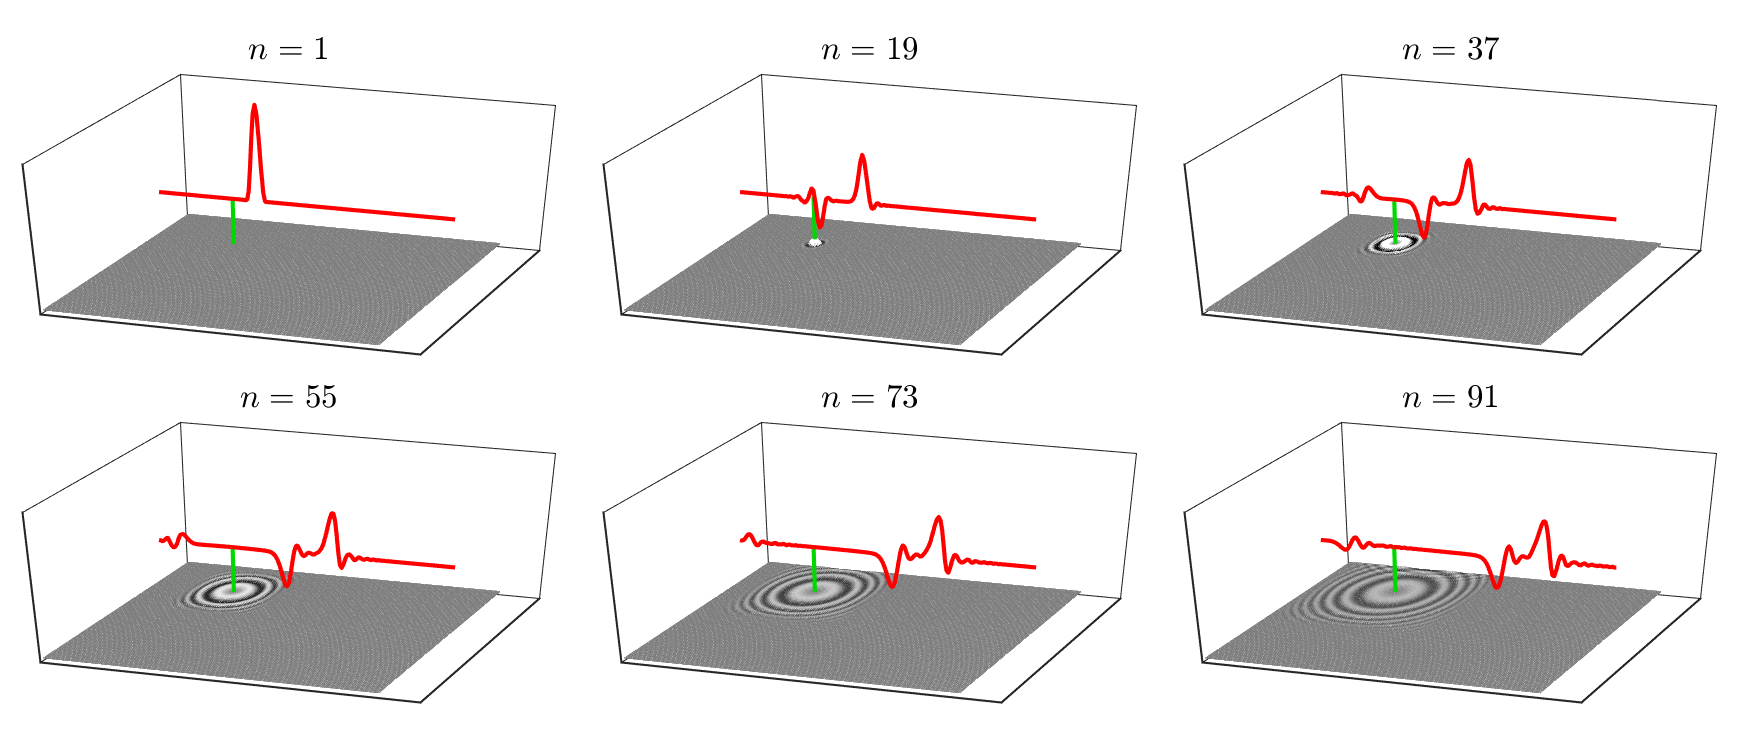
\includegraphics[width=\textwidth]{figures/interactions/stringPlate.eps}
    \caption{A visualisation of string-plate system. The string is shown in red, the plate in gray and the connection in green. \label{fig:stringPlate}}
\end{figure}

In the following, the $\i$ and $\j$ vectors are used as in Section \ref{sec:matrixFormRigid} and are of the appropriate sizes. The matrices for the string can be found in Eq. \eqref{eq:matrixFormStiffString} and those for the plate in Eq. \eqref{eq:matrixFormThinPlate}. When implementing connections (or any other interactions for that matter), one mostly performs the following steps in the main loop:
\begin{enumerate}
    \item Calculate entire scheme without force terms:\\
    \vspace{-0.5em}\begin{equation*}
        \u^\star = (\B_\stxt\u^n + \C_\stxt\u^{n-1}) / A_\stxt, \qaq \w^\star = (\B_\ptxt\w^n + \C_\ptxt\w^{n-1})/A_\ptxt
    \end{equation*}
    \item Obtain $u^\star$ and $w^\star$:\\
    \vspace{-1em}\begin{equation*}
       u^\star = \i_u \u^\star, \qaq w^\star = \i_w \w^\star
    \end{equation*}
    \item Calculate the connection force $f^n$ (Eq. \eqref{eq:stringPlateForce}).
    \item Add force terms to the schemes without connection forces:\\
    \begin{equation*}
        \u^{n+1} = \u^{\star} - \j_u \frac{f^n k^2}{\rho_\stxt A (1+\szX[\stxt])},\qaq \w^{n+1} = \w^{\star} + \j_w \frac{f^n k^2}{\rho_\ptxt H (1+\szX[\ptxt])}
    \end{equation*} 
\end{enumerate}

\subsection{Energy analysis}
Recalling the total energy and damping terms for the string and plate in Sections \ref{sec:energyAnalysisString} and \ref{sec:energyAnalysisThinPlate} respectively, one can --  similar to Eq. \eqref{eq:rOCconnSystem} -- arrive at the following:
\begin{equation}
    \dtp(\h_\stxt + \h_\ptxt) + \q_\stxt + \q_\ptxt = -\Iq (\dtd \uqn)f^n +\Ilm(\dtd \wlmn)f^n
\end{equation}
which can be rewritten to
\begin{equation*}
    \dtp(\h_\stxt + \h_\ptxt) + \q_\stxt + \q_\ptxt = -\dtd \left(\Iq \uqn - \Ilm\wlmn\right)f^n.
\end{equation*}
Substituting the definitions for $f^n$ and $\eta^n$ from Eqs. \eqref{eq:discForceStringPlate} and \eqref{eq:discEtaStringPlate} respectively, yields
\begin{equation*}
    \dtp(\h_\stxt + \h_\ptxt) + \q_\stxt + \q_\ptxt = -(\dtd\eta^n)(K_1\mtt\eta^n+K_3(\eta^n)^2\mtd\eta^n+R\dtd\eta^n).
\end{equation*}
Due to the nonlinear dependency on $\eta^n$ one must isolate $\dtp$ from the nonlinear term manually, according to
\begin{align*}
    &\ \ K_3(\eta^n)^2(\dtd \eta^n)(\mtd \eta^n),\\
    = &\ \ \frac{K_3(\eta^2)}{2k}(\eta^{n+1} - \eta^{n-1})\frac{1}{2}(\eta^{n+1} + \eta^{n-1}),\\
    = &\ \ \frac{K_3(\eta^n)^2}{4k}\left((\eta^{n+1})^2 - (\eta^{n-1})^2\right),\\
    = &\ \ \frac{K_3}{4k}\left((\eta^{n+1}\eta^n)^2 - (\eta^n\eta^{n-1})^2\right),\\
    = &\ \ \dtp\left(\frac{K_3}{4}(\eta^n\eta^{n-1})^2\right).
\end{align*}
% \begin{equation*}
%     (\dtd \eta^n)K_1\mtt\eta^n \quad \xRightarrow{\text{Eq. \eqref{eq:prodIdentity5}}} \quad \frac{K_1}{8}(\eta^n+\eta^{n-1})^2 
% \end{equation*}
Finally, using identity \eqref{eq:prodIdentity5} for the linear term, the following balance follows
\begin{equation}
    \dtp(\h_\stxt + \h_\ptxt + \h_\ctxt) = - \q_\stxt - \q_\ptxt - \q_\ctxt,
\end{equation}
where the energy stored by the spring connection is
\begin{equation*}
    \h_\ctxt = \frac{K_1}{8}(\eta^n+\eta^{n-1})^2 + \frac{K_3}{4}(\eta^n\eta^{n-1})^2
\end{equation*}
and the damping term of the connection is
\begin{equation*}
    \q_\ctxt = R(\dtd\eta^n)^2.
\end{equation*}
Figure \ref{fig:energyStringPlate} shows the energetic output of the string-plate system corresponding to Figure \ref{fig:stringPlate}. One can observe that, due to the high value for spring-damping $R$, the total energy decreases substantially as the excitation reaches the connection location along the string. 

\begin{figure}[h]
    \centering
    \begin{tikzpicture}[->,node distance=3cm,
        thick,main node/.style={circle,draw}]
    
        \node[] (image) at (0,0) {
        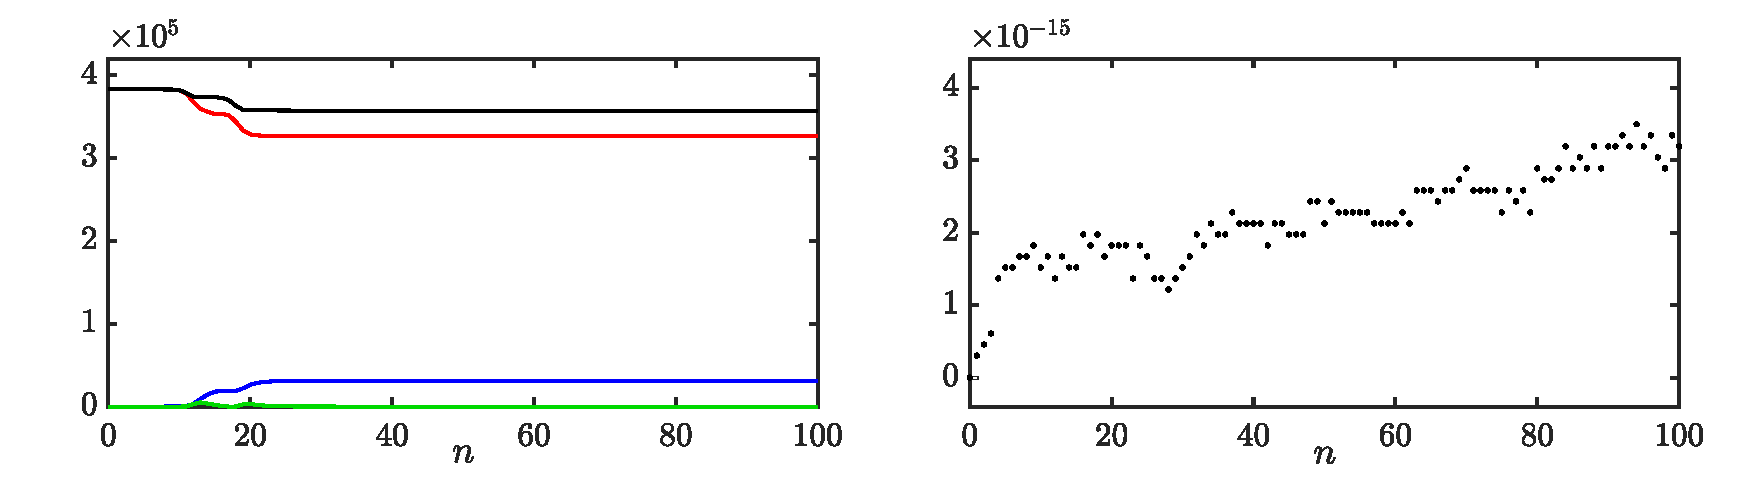
\includegraphics[width=\textwidth]{figures/interactions/stringPlateEnergy.eps}
        };
    
        \node[] (he) at (0.2,0.5) {\small $\mathfrak{h}_\text{e}$};

        \node[] (h) at (-5.8, 1) {\small $\mathfrak{h}$};
        \node[] (v) at (-5.8, 0.5) {\small $\color{red}\mathfrak{h}_\stxt$};
        \node[] (t) at (-5.8, 0) {\small $\color{blue}\mathfrak{h}_\ptxt$};
        \node[] (c) at (-5.8, -0.5) {\small $\color[HTML]{00DB00}\mathfrak{h}_\ctxt$};

      \end{tikzpicture}
      \caption{The energy of the string (red), the plate (blue), the spring (green) and the total energy (black) of the connected string-plate system \eqref{eq:connStringPlateFDSs}. The energy corresponds to the system in Figure \ref{fig:stringPlate}. The right panel shows the normalised energy (according to Eq. \eqref{eq:normalisedEnergyDamping}) shows that the deviation of the energy is within machine precision. \label{fig:energyStringPlate}}
\end{figure}

% \subsection{Non-dimensional}
% The scaled system can be written as:
% \begin{align}
%     \ptt u &= \gamma^2 \pxx u - \kappa_\stxt^2 \pxxxx u - 2\szX[\stxt]\pt u + 2\soX[\stxt] \pt\pxx u - \delta(x-x_\ctxt)F\\
%    \pt w &= -\kappa_\ptxt^2\Delta\Delta w - 2\szX[\ptxt]\pt w + 2\soX[\ptxt] \pt\pxx w + \delta(x-x_\ctxt, y-y_\ctxt)F
% \end{align}
% where
% \begin{equation}
%     F = F(t) = \omega_1^2\eta+\omega_3^4\eta^3+\sigma_\ctxt \dot\eta
% \end{equation}
% and
% \begin{equation}
%     \eta = \eta(t) = u(x_\ctxt, t) - w(x_\ctxt, y_\ctxt, t)
% \end{equation}


% \begin{equation}
%     I(x_\ctxt)\delta_{tt}\uqn = c^2
%     \left(I(x_\ctxt)\dxx\uqn\right) + I(x_\ctxt)J(x_\ctxt)F
% \end{equation}


% \subsubsection{Relative location of objects}\todo{look at this compared to when I talk about it in chapter \ref{ch:collisions}}


% Forces should be equal and opposite. 

% % \part{Real-Time Implementation and Control}\label{part:realtime}
% % \chapter*{Resonators}
<<<<<<< HEAD
Though the physical models described in the previous part are also considered resonators, they are \textit{ideal} cases. In other words, you would not be able to find these ``in the wild'' as they do not includes effects such as losses or frequency dispersion. 

This part presents the different resonators used over the course of the project and is structured as follows: Chapter \ref{ch:stiffString} introduces the stiff string, a model which has been used a lot over the course of this project, Chapter \ref{ch:brass} talks about brass instruments, or more generally, 1D systems of varying geometry along their spatial dimension. Finally, Chapter \ref{ch:2Dsyst} will introduces 2D systems which, in this project, have been used to simulate (simplified) instrument bodies.
=======
Although the physical models described in the previous part -- the simple mass-spring system and the 1D wave equation -- are also considered resonators, they are \textit{ideal} cases. In other words, these can not be found in the real world as effects such as losses or frequency dispersion are not included. 

This part presents the different resonators used over the course of the project that better include these non-ideal physical processes and is structured as follows: Chapter \ref{ch:stiffString} introduces the stiff string, an extension of the 1D wave equation, % and is the single most-used model in this project. 
Chapter \ref{ch:brass} introduces acoustic tubes, used to model brass instruments, and finally, Chapter \ref{ch:2Dsyst} introduces 2D systems which, in this project, have been used to simulate (simplified) instrument bodies. The analysis techniques introduced in the previous part will be applied to all models and described in detail. 
>>>>>>> master

\input{realtime/realtimeImp}
\chapter{Control}

\section{Sensel Morph}
150 Hz

\section{Phantom OMNI}

% \part{Contributions}\label{part:contributions}
% \chapter*{Resonators}
<<<<<<< HEAD
Though the physical models described in the previous part are also considered resonators, they are \textit{ideal} cases. In other words, you would not be able to find these ``in the wild'' as they do not includes effects such as losses or frequency dispersion. 

This part presents the different resonators used over the course of the project and is structured as follows: Chapter \ref{ch:stiffString} introduces the stiff string, a model which has been used a lot over the course of this project, Chapter \ref{ch:brass} talks about brass instruments, or more generally, 1D systems of varying geometry along their spatial dimension. Finally, Chapter \ref{ch:2Dsyst} will introduces 2D systems which, in this project, have been used to simulate (simplified) instrument bodies.
=======
Although the physical models described in the previous part -- the simple mass-spring system and the 1D wave equation -- are also considered resonators, they are \textit{ideal} cases. In other words, these can not be found in the real world as effects such as losses or frequency dispersion are not included. 

This part presents the different resonators used over the course of the project that better include these non-ideal physical processes and is structured as follows: Chapter \ref{ch:stiffString} introduces the stiff string, an extension of the 1D wave equation, % and is the single most-used model in this project. 
Chapter \ref{ch:brass} introduces acoustic tubes, used to model brass instruments, and finally, Chapter \ref{ch:2Dsyst} introduces 2D systems which, in this project, have been used to simulate (simplified) instrument bodies. The analysis techniques introduced in the previous part will be applied to all models and described in detail. 
>>>>>>> master

\chapter{Dynamic Grid}\label{ch:dynamicGrid}

\textit{Often in math, you should view the definition not as a starting point, but as a target. Contrary to the structure of textbooks, mathematicians do not start by making definitions and then listing a lot of theorems, and proving them, and showing some examples. The process of discovering math typically goes the other way around. They start by chewing on specific problems, and then generalising those problems, then coming up with constructs that might be helpful in those general cases,and only then you write down a new definition (or extend an old one). - Grant Sanderson (AKA 3Blue1Brown) https://youtu.be/O85OWBJ2ayo?t=359}

This chapter provides an extended summary to the paper ``Dynamic grids for Finite-Difference Schemes in Musical Instrument Simulations'' \citeP[G]. The paper presents a novel method to smoothly add and remove grid points from a FD scheme which allows for dynamic parameter variations without compromising stability or quality of the simulation (see Section \ref{sec:quality1DWave}). 

After a brief introduction  and summary of the method, the chapter will extend on paper \citeP[G] by providing some design considerations as a result of iterations done as well as providing details on the implementation of the displacement correction and the modal analysis shown in the paper. 

\section{Background and motivation}
Simulating musical instruments using physical modelling -- as mentioned in Chapter \ref{ch:physMod} -- allows for manipulations of the instrument that are impossible in the physical world. Examples of this are changes in material density or stiffness, cross-sectional area (1D), thickness (2D) and size of the system in general. 



\subsection{Examples}
Apart from being potentially sonically interesting, there are examples in the physical world where certain aspects of the instrument are manipulated in real-time.

Tension in a string is changed when tuning it

Some artists even use this in their performances \cite{Gomm2011, Mayer2008}
Or gr4yhound: https://www.youtube.com/watch?v=fSQ9Dg65EFo

The hammered dulcimer is another example where the strings are tensioned over a bridge where one can play the string at one side of the bridge, while pushing down on the same string on the other side \cite{Glenn2014}.

\noindent 1D:
\begin{itemize}
    \item Trombone
    \item Slide whistle
    \item Guitar strings
    \begin{itemize}
        \item Fretting finger pitch bend
        \item Above the nut \cite{Mayer2008}
        \item Tuning pegs directly \cite{Gomm2011}
    \end{itemize}
    \item Hammered dulcimer \cite{Glenn2014}
    \item Erhu? 
\end{itemize}
%
2D: 
\begin{itemize}
    \item Timpani
    \item Bodhr\'an: https://youtu.be/b9HyB5yNS1A?t=146
    \item Talking drum (hourglass drum): https://youtu.be/B4oQJZ2TEVI?t=9
    \item Flex-a-tone (could also be 1D tbh..): https://www.youtube.com/watch?v=HEW1aG8XJQk.
\end{itemize}

A more relevant example is that of the trombone, where the size of the instrument is changed in order to play different pitches. Modelling this using FDTD methods would require

% \section{Issues with FDTD methods}


In his thesis, Harrison points out that in order to model the trombone, grid points need to be introduced 


Something about time-dependent variable coefficient Stokes flow:
https://arxiv.org/abs/1010.2832

Time-varying propagation speed in waveguides: https://quod.lib.umich.edu/cgi/p/pod/dod-idx/fractional-delay-application-time-varying-propagation-speed.pdf?c=icmc;idno=bbp2372.1997.069;format=pdf

Special boundary conditions (look at!):
Modeling of Complex Geometries and Boundary Conditions in Finite Difference/Finite Volume Time Domain Room Acoustics Simulation (\url{https://www.researchgate.net/publication/260701231_Modeling_of_Complex_Geometries_and_Boundary_Conditions_in_Finite_DifferenceFinite_Volume_Time_Domain_Room_Acoustics_Simulation})



\section{Summary}
The variations are assumed to be at sub-audio rate (i.e., human gestural control) so that analysis techniques are still valid to some degree.


Consider the 1D wave equation  as presented in Section \ref{sec:1DWave}, describing the motion of a system of length $L$, its state described by $q = q(x,t)$ defined for $t\geq 0$ and $x\in\D$ with domain $\D = [0, L]$. This state variable can be discretised to a grid function $\qln$ with $n\in \mathbb{N}^0$ and $l \in \{0, \hdots, N\}$ with $N$ being tthe number of intervals between the grid points. The PDE in \eqref{eq:1DwavePDE} can then be discretised to the following FD scheme
\begin{equation}
    \dtt \qln = c^2\dxx \qln.
\end{equation}

Rather than working with this scheme directly, paper \citeP[G] proposes to split it into two to get the following system 
\begin{subequations}
    \begin{equation}
        \dtt \ulun = c^2\dxx \ulun,
        \dtt \wlwn = c^2\dxx \wlwn.
    \end{equation}
\end{subequations}

\section{Iterations}
Iterations have been:
\begin{itemize}
    \item Interpolated boundary conditions
    \item Linear interpolation
\end{itemize}

\todo{These sections are taken from the JASA appendix} In this appendix, some iterations done over the course of this project will be shown in more detail. In the following, the 1D wave equation with a wave speed of $c = 1470$ m/s, a length of $L = 1$ m, Dirichlet boundary conditions and a sample rate of $f_\text{s} = 44100$ Hz is considered, and -- through Eq. \eqref{eq:compactLambda} -- satisfies the CFL condition with equality. These values result in $N = 30$, or a grid of 31 points including the boundaries. Then, the wave speed is decreased to $c \approx 1422.6$ m/s, i.e., the wave speed that results in $N=31$ and satisfies the stability condition with equality again. 

\subsection{Full-grid interpolation}
One way to go from one grid to another is performing a full-grid interpolation \cite[Chap. 5]{theBible}. If the number of points changes according to Eq. \eqref{eq:orderOfCalcGrid}, i.e., if $N^n \neq N^{n-1}$ the full state of the system ($u_l^n, u_l^{n-1}\ \forall l$)  can be interpolated to the new state. See Figure \ref{fig:fullGrid}. 

\begin{figure}[ht]
    \centering

%% \reprintcolumnwidth is the same in preprint and reprint for
%% ease of use for authors:
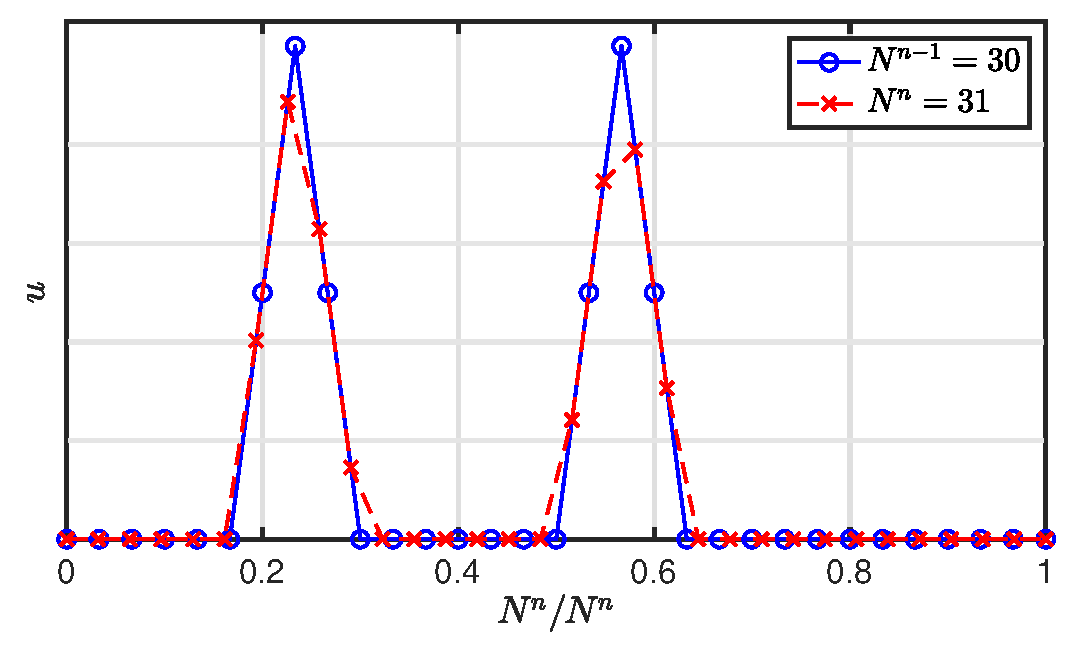
\includegraphics[width=0.5\textwidth]{figures/contributions/dynamicgrid/fullGrid.eps}
\caption{\label{fig:fullGrid}{Upsampling $u$ (with an arbitrary state) using (linear) full-grid interpolation with $N^{n-1} = 30$ and $N^n = 31$. The horizontal axis is normalised with respect to $N^n$.}}
\end{figure} 

An issue that arises using this method is that the Courant number $\lambda$ will slightly deviate from the CFL condition as $c$ changes. Using Eq. \eqref{eq:compactLambda} with $L/ck$ approaching $31$ (from below), the minimum value of $\lambda \approx 30/31 \approx 0.9677$.
%\footnote{Eq. \eqref{eq:orderOfCalcGrid} can be compactly rewritten as $\lambda = \frac{ck}{L}\cdot \text{floor}\left(\frac{L}{ck}\right)$. As $L/ck$ approaches $31$ (from below), $\lambda \approx \frac{30}{31}$.}
This, employing Eq. \eqref{eq:fmax}, has a maximum frequency output of $f_\text{max} \approx 18,475$ Hz. 
%For slightly lower values of $c$, $N = 31$ and $\lambda \approx 1$. 
The Courant number will deviate more for higher values of $c$ and thus lower values for $N$ -- for instance, if $N$ approaches $11$ (from below), $\lambda \approx 10/11 \approx 0.9091$ and $f_\text{max} \approx 16,018$ Hz.

Another problem with full-grid interpolation, is that it has a low-passing effect on the system state, and thus on the output sound. %Figure \ref{fig:fullGrid} shows the biggest changes are in the state are at the locations with the biggest difference between the states of consecutive grid points.
Furthermore, this state-interpolation causes artefacts or `clicks' in the output sound as the method causes sudden variations in the states.  

All the aforementioned issues could be solved by using a (much) higher sample rate and thus more grid points, but this would render this method impossible to work in real time.

\subsection{Adding and removing points at the boundary}\label{sec:addAtBoundary}
To solve the issues exhibited by a full-grid interpolation, points can be added and removed at a single location and leave most points unaffected by the parameter changes. A good candidate for a location to do this is at a fixed (Dirichlet) boundary. The state $u$ at this location is always $0$ so points can be added smoothly. 

As $c$ decreases, $h$ can be calculated according to Eq. \eqref{eq:orderOfCalcGrid} and decreases as well.

This has a physical analogy with tuning a guitar string. Material enters and exits the neck (playable part of the string) at the nut, which in discrete time means grid points appearing and disappearing at one boundary.

To yield smooth changes between grid configurations, an interpolated boundary has been developed, the possibility of which has been briefly mentioned in \cite[p. 145]{theBible}. The Dirichlet condition in Eq. \eqref{eq:contDirichlet} can be extended to be the simply supported boundary condition:
\begin{equation}
    u(x, t) = \frac{\partial^2}{\partial x^2}u(x, t) = 0 \quad \text{where} \quad x = 0, L,
\end{equation}
or, when discretised,
\begin{equation}\label{eq:simplySupportedDiscrete}
    u_l^n = \delta_{xx}u_l^n = 0, \quad \text{where} \quad l = 0, N.
\end{equation}
This means that on top of that the state of the boundary should be $0$, the curvature around it should also be $0$. One can again solve for the virtual grid points at the boundary locations, yielding
\begin{equation}
    u_{-1}^n = -u_1^n \quad \text{and} \quad u_{N+1}^n = -u_{N-1}^n.
\end{equation}
This is visualised in Figure \ref{fig:simplySupportedBound}.

\begin{figure}
    \centering
    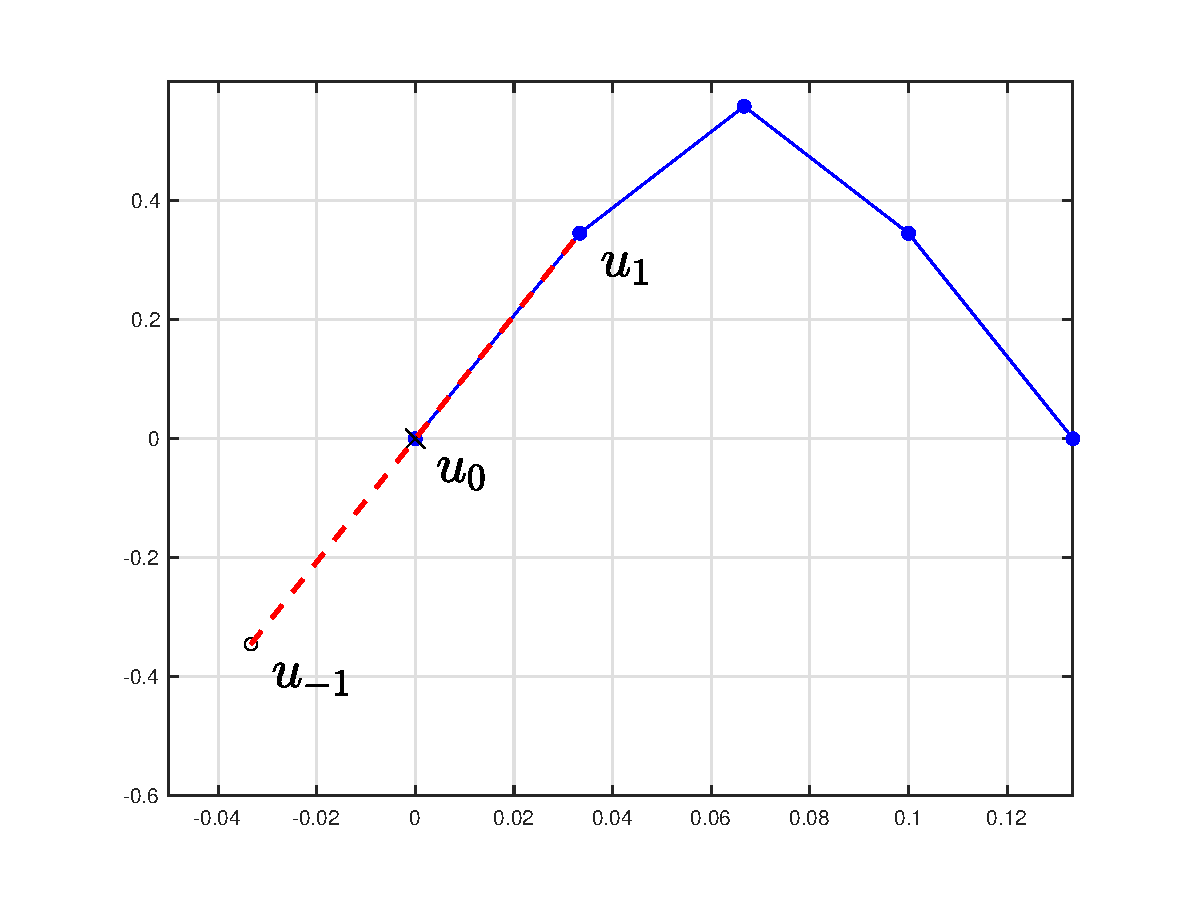
\includegraphics[width=0.7\textwidth]{figures/contributions/dynamicgrid/simplySupportedBoundary.eps}
    \caption{\label{fig:simplySupportedBound}{The simply supported boundary condition: both the state and the curvature at the boundary -- at $l=0$ -- should be $0$.}}
\end{figure} 

If the flooring operation in Eq. \eqref{eq:numberOfIntervals} is removed this introduces a fractional number of grid points.


The by-product of using a fractional $N$ this is that the CFL condition in \eqref{eq:CFL} can now always be satisfied with equality no matter what the wave speed is.

An issue with this method is that removing points is much harder than adding.

their interactions change through a change in the grid spacing and wave speed. This interaction, though, is defined by $\lambda$ which 

\begin{figure}
    \centering
%% \reprintcolumnwidth is the same in preprint and reprint for
%% ease of use for authors:
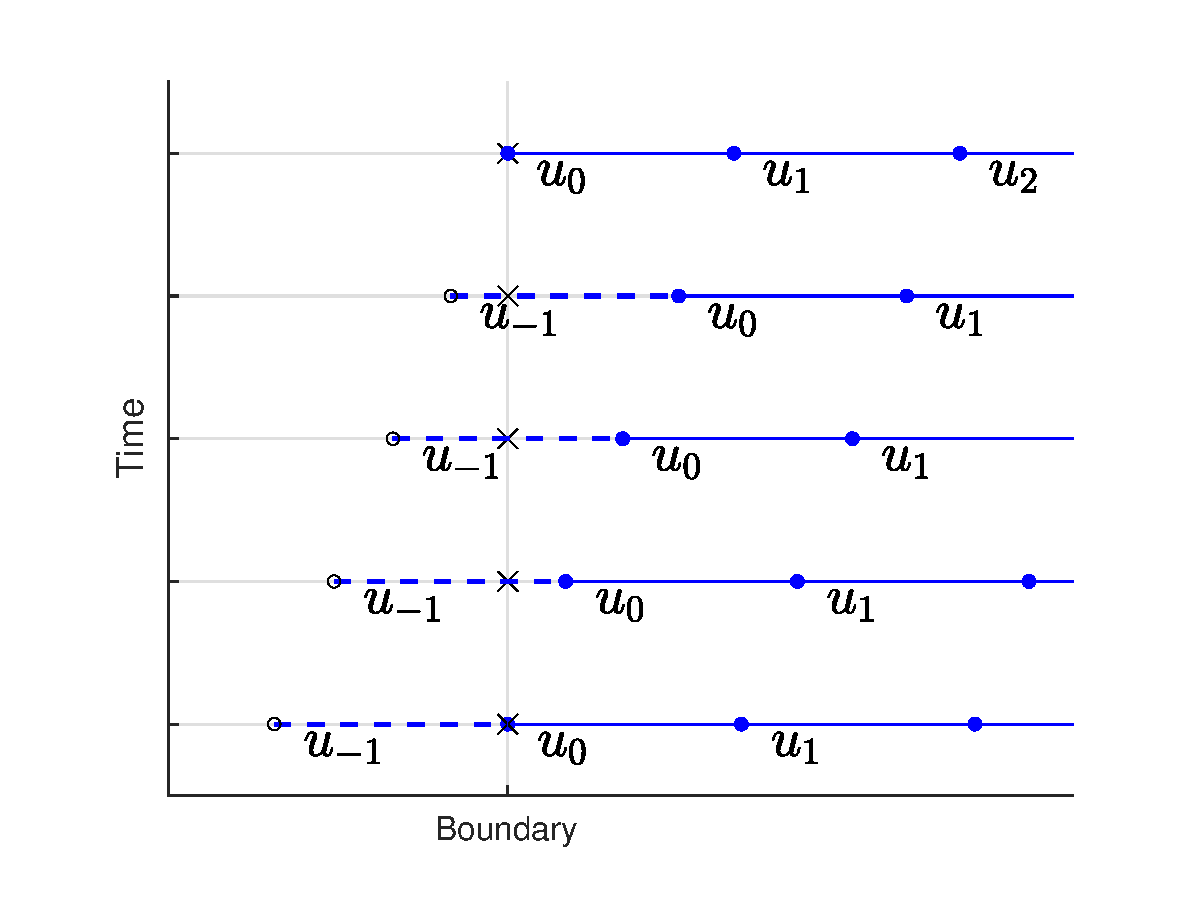
\includegraphics[width=0.7\textwidth]{figures/contributions/dynamicgrid/boundaryGrid.eps}
\caption{\label{fig:changingBoundary}{The grid changing over time}}
\end{figure}

\subsection{Cubic interpolation}

\subsection{Sinc interpolation}


\section{Displacement correction implementation} 
One detail that was not provided in paper \citeP[G], is the impelmentation of the displacement correction.
When the wave speed is increased and points are removed, it is not necessarily true that $u_M = w_0$ at the time of removal and the rigid connection in \eqref{eq:rigid} is violated. On top of the virtual grid point ``generation'' from the interpolation described above, one could add a connection force that is dependent on how close the inner boundaries $u_M$ and $w_0$ are.

Equation \eqref{eq:systemHalfStrings} can be extended to include a spring force between $u_M$ and $w_0$ as
\begin{equation}\label{eq:dispCorrSyst}
    \begin{cases}
        \delta_{tt}u^n &= c^2\delta_{xx}u^n + J(x_{u_M})F\\
        \delta_{tt}w^n &= c^2\delta_{xx}w_0^n - J(x_{w_0})F
    \end{cases}
\end{equation}
with 
\begin{equation}\label{eq:corrForceNoDamp}
    F = \beta \mu_{t\cdot}\eta^n.
\end{equation}
Here,
\begin{equation}\label{eq:etaCorrDef}
    \eta^n \triangleq w_0^n - u_M^n
\end{equation}
is the difference in displacement between the inner boundaries
and $\beta = \beta(\alpha)$ 
acts as a spring coefficient that is a function of the distance between the inner boundaries along the grid, i.e., $\alpha$. Furthermore, the centred temporal averaging operator $\mu_{t\cdot}$ is used in \eqref{eq:corrForceNoDamp} to ensure stability \cite{Bilbao2009Modular}.

We then continue by finding a definition for $\beta$ that is inversely proportional to $\alpha$, i.e., the smaller $\alpha$ is the higher the `correction' effect, ideally approaching an infinite stiffness, or rigid connection, when $\alpha = 0$ and no stiffness when $\alpha \rightarrow 1$. This can be achieved by defining $\beta = \beta(\alpha)$ as
\def\plusEps{+ \epsilon}
% \def\plusEps{};
\def\alfPlusEps{(\alpha \plusEps)}
% \def\alfPlusEps{\alpha}
\begin{equation}\label{eq:betaDef}
    \beta = \frac{1 - \alpha}{\alpha \plusEps},
\end{equation}
with $0<\epsilon \ll 1$ to prevent a division by 0. It will be shown that when calculating the force after expansion, a division by 0 can be prevented and $\epsilon = 0$ will still yield a defined solution. We can observe that when $\alpha = 0$ and the correction effect needs to be at a maximum, $\beta\rightarrow \infty$. When $\alpha \rightarrow 1$, $\beta \rightarrow 0$.

We can also add a damping term to \eqref{eq:corrForceNoDamp} which is also scaled by $\beta$ as
\begin{equation}\label{eq:corrForce}
    F = \beta \left(\mu_{t\cdot}\eta^n +\sigma_0\delta_{t\cdot}\eta^n \right),
\end{equation}
where $\sigma_0$ is the damping coefficient. Then, we can solve for $\eta^{n+1}$ 
\begin{align}
    F &= \beta\left(\frac{1}{2}\left(\eta^{n+1}+\eta^{n-1}\right) + \frac{\sigma_0}{2k}\left(\eta^{n+1}-\eta^{n-1}\right)\right)\nonumber\\
    F&= \left(\frac{\beta (1 + \sigma_0/k)}{2}\right)\eta^{n+1} + \left(\frac{\beta (1 - \sigma_0/k)}{2}\right) \eta^{n-1}\nonumber\\
    \xLeftrightarrow{\mystrut\ \text{Eq. \eqref{eq:betaDef}}\ } \quad \eta^{n+1} &= \left(\frac{2
    \alfPlusEps}{(1+\sigma_0/k)(1-\alpha)}\right)F - \underbrace{\frac{1-\sigma_0/k}{1+\sigma_0/k}}_{r}\eta^{n-1}.\label{eq:etaSolut1}
\end{align}
Using superscript $\text{I}$ to denote an intermediate state describing of $u^{n+1}_M$ and $w^{n+1}_0$ without the connection force (see \eqref{eq:resultOneConnectedPoint}), we also know, through Eq. \eqref{eq:etaCorrDef}, that 

\begin{align}
    \eta^{n+1} &= w_0^\text{I}-\frac{k^2}{h}F-\left(u_M^\text{I}+\frac{k^2}{h}F\right)\nonumber\\
    \eta^{n+1} &= w_0^\text{I} - u_M^\text{I} - \frac{2k^2}{h}F,\label{eq:etaNext}
\end{align}
which can be set equal to \eqref{eq:etaSolut1} and solved for $F$ according to 

\begin{align*}
    \left(\frac{2
    \alfPlusEps}{(1+\sigma_0/k)(1-\alpha)}\right)F - r \eta^{n-1} &= w_0^{I} - u_M^{I}- \frac{2k^2}{h}F\\
    \left(\frac{2h
    \alfPlusEps + 2k^2(1+\sigma_0/k)(1-\alpha)}{h(1+\sigma_0/k)(1-\alpha)}\right)F &= w_0^{I} - u_M^{I}+r\eta^{n-1}\\
    F &= \left(w_0^{I} - u_M^{I}+r\eta^{n-1}\right)\left(\frac{h(1+\sigma_0/k)(1-\alpha)}{2h \alfPlusEps + 2k^2(1+\sigma_0/k)(1-\alpha)}\right).
\end{align*}
It is clear now that no matter the value of $\alpha$, no division by 0 will occur, so $\epsilon = 0$ is still defined. The final equation for $F$ can thus be written as
\begin{equation}\label{eq:finalForce}
    F = \left(w_0^{I} - u_M^{I}+r\eta^{n-1}\right)\underbrace{\left(\frac{h(1+\sigma_0/k)(1-\alpha)}{2h\alpha + 2k^2(1+\sigma_0/k)(1-\alpha)}\right)}_{\Psi}.
\end{equation}
This can then be filled into \eqref{eq:dispCorrSyst} and used to get $u_M^{n+1}$ and $w_0^{n+1}$ respectively. \SWcomment[Using $\alpha = 0$ and $\sigma_0 = 0$ as a test case to see what would happen to the scheme at the inner boundaries when they perfectly overlap (and without damping, just restoring force), we get that $r = 1$ and \eqref{eq:finalForce} becomes
\begin{align*}
    F &= \left(w_0^{I} - u_M^{I}+\eta^{n-1}\right)\left(\frac{h}{2k^2}\right)\\
    \xLeftrightarrow{\mystrut\ \text{Eq. \eqref{eq:etaNext}}\ } \quad F &= \left(\eta^{n+1} + \frac{2k^2}{h}F + \eta^{n-1}\right)\left(\frac{h}{2k^2}\right)\\
    F - F &= \eta^{n+1} + \eta^{n-1}\\
    2\mu_{t\cdot}\eta^n &= 0\\
    \mu_{t\cdot}\eta^n &= 0
\end{align*}
showing that when $\alpha = 0$, the $\eta^n$ should be 0 and thus boils down to a rigid connection.]

\subsubsection{Modal analysis}
Due to the damping that is present in the system, it needs to be written in one-step form. Recalling \eqref{eq:uVecDef} we can write \eqref{eq:dispCorrSyst} in vector-matrix form
\begin{equation}\label{eq:formForOneStep}
    \A \U^{n+1} = \B \U^n + \C\U^{n-1}
\end{equation}
and rewrite to one-step form as \SWcomment[decapitalise u!]
\begin{equation}\label{eq:oneStepFormDynamicGrid}
    \underbrace{\begin{bmatrix}
        \U^{n+1}\\
        \U^n
    \end{bmatrix}}_{\mathbf{W}^{n+1}} = 
    \underbrace{\begin{bmatrix}
        \A^{-1}\B & \A^{-1}\C\\
        \I & \mathbf{0}
    \end{bmatrix}}_{\Q}
    \underbrace{\begin{bmatrix}
        \U^n\\
        \U^{n-1}
    \end{bmatrix}}_{\mathbf{W}^n}
\end{equation}

The most straightforward way to obtain the matrices, is to expand the forces in system \eqref{eq:dispCorrSyst} directly. 
% \begin{equation}
%     \begin{cases}
%         \delta_{tt}u^n &= c^2\delta_{xx}u^n + J(x_{u_M})\frac{\beta}{2}(\eta^{n+1} + \eta^{n-1} + \sigma_0/k (\eta^{n+1} - \eta^{n-1}))\\
%         \delta_{tt}w^n &= c^2\delta_{xx}w_0^n - J(x_{w_0})\frac{\beta}{2}(\eta^{n+1} + \eta^{n-1} + \sigma_0/k (\eta^{n+1} - \eta^{n-1}))
%     \end{cases}
% \end{equation}
% and
Recalling $\U$ from \eqref{eq:uVecDef} (of size $\mathcal{M} = M+M_w$) and including the virtual grid point definitions encapsulated in $\B_2$, we can rewrite the system to
\begin{equation}
    \I\U^{n+1} = \B_2\U^n - \I\U^{n-1} + (\J\boldsymbol{\eta})\frac{\beta k^2}{2}\left((1+\sigma_0/k)\U^{n+1} + (1-\sigma_0/k)\U^{n-1}\right)
\end{equation}
where 
\begin{equation}
    \J = [\mathbf{0}_{M-1}, 1/h, -1/h, \mathbf{0}_{M_w-1}]^T
\end{equation}
where $\mathbf{0}_i$ is a row-vector of zeros with length $i$ and
\begin{equation}
    \boldsymbol{\eta} = [\mathbf{0}_{M-1}, -1, 1, \mathbf{0}_{M_w-1}].
\end{equation}
vectorising the effect of \eqref{eq:etaCorrDef} on $\U$. Note that as $\J$ is a column vector and $\boldsymbol{\eta}$ a row vector, the multiplication of the two yields an $\mathcal{M}\times\mathcal{M}$ matrix.

Then refactoring to the form in \eqref{eq:formForOneStep} and using identity matrix $\I$ with size $\mathcal{M} \times \mathcal{M}$ yields the following matrices
% \begin{equation}
%     \underbrace{\left(\I - \frac{\beta k^2 (1+\sigma_0/k)}{2}\J\boldsymbol{\eta}\right)}_{\A}\U^{n+1} = \underbrace{\mathbf{B}_2}_{\B}\U^n +\underbrace{\left(- \I - \frac{\beta k^2 (1-\sigma_0/k)}{2}\J\boldsymbol{\eta}\right)}_{\C} \U^{n-1}
% \end{equation}

\begin{equation}
    \A = \I - \frac{\beta k^2 (1+\sigma_0/k)}{2}\J\boldsymbol{\eta}, \qquad \B = \mathbf{B}_2, \qquad \text{and} \qquad \C = -\left(\I - \frac{\beta k^2 (1-\sigma_0/k)}{2}\J\boldsymbol{\eta}\right)
\end{equation}
Although substituting these definitions into \eqref{eq:oneStepFormDynamicGrid} gives an identical result to the matrix definitions above (comparisons show a difference between the $\Q$ matrices around machine precision), $\beta$ can still go to infinity. In this case, $\epsilon \neq 0$ in \eqref{eq:betaDef}. 

\section{%Modal 
Analysis and experiments}
\subsection{Interpolation technique}
\subsection{Interpolation range}
\subsection{Location}
... where to add and remove points

Using the whole range, we can still add/remove points at the sides. 

\section{Discussion and conclusion}\label{sec:conclusion}
\chapter{Large Scale Modular Physical Models}\label{ch:largeScale}
This chapter provides an extended summary for the work presented in the papers ``Real-Time Control of Large-Scale Modular Physical Models using the Sensel Morph'' \citeP[A] and ``Physical Models and Real-Time Control with the Sensel Morph'' \citeP[B].  Paper \citeP[A] presents the work done on various physical models connected by nonlinear springs using three instruments as case studies: the esraj (bowed sitar), the hammered dulcimer and the hurdy gurdy. The implementations and a video showcasing the hurdy gurdy can be found online.\footnote{\url{https://github.com/SMC-AAU-CPH/ConnectedElements/releases/tag/v5.0}}\textsuperscript{,}\footnote{\url{https://youtu.be/BkxLji2ap1w}} Paper \citeP[A] follows \cite{theBible} and \cite{Bilbao2009Modular} and uses `scaling' (see Section \ref{sec:1DwaveContTime}). To relate the paper to the theory presented in this thesis, this chapter presents the models in a non-scaled, dimensional form. The eventual implementation of the models is equivalent. Then, a summary of the remaining parts of the paper is provided, including descriptions of the instruments.
% Furthermore, this chapter will build on the contents of paper \citeP[A] by providing more details on the implementation.\todo{will it though?}

\section{Physical models}\label{sec:modelsLargeScale}
All instruments use multiple instances of the stiff string presented in Chapter \ref{ch:stiffString} and one instance of the thin plate presented in Section \ref{sec:thinPlate}. The latter was used as a simplified instrument body for the resulting simulations (see Section \ref{sec:largeScaleInstruments}). Theory on connections can be found in Chapter \ref{ch:connections}, and information on the string-plate connection specifically, is presented in Section \ref{sec:stringPlateConnection}.

Consider a set of strings, where the transverse displacement of string $s$ is described by $u_s = u_s(\chi_s, t)$ (in m) defined for $t\geq 0$ and $\chi_s \in \D_s$ for domain $\D_s = [0, L_s]$ and length $L_s$ (in m). Notice that every string is defined for a separate coordinate system $\chi_s$. In the following, spatial derivatives $\partial_{\chi_s}$ are the same as those described in Section \ref{sec:FDoperators}, but with respect to coordinate $\chi_s$ (similar to Chapter \ref{ch:connections}). The PDE of string $s$ with an external connection force is defined as %(after division by $\rho_sA_s$)
\begin{equation}
    \ptt u_s = c_s^2 \partial_{\chi_s}^2 u_s - \kappa_s^2 \partial_{\chi_s}^4 u_s - 2 \szX[s]\pt u_s + 2 \soX[s] \partial_{\chi_s}^2 u_s - \delta(\chi_s - \chi_{s, \ctxt})\frac{f_s}{\rho_sA_s},
\end{equation}
where spatial Dirac delta function $\delta(\chi_s - \chi_{s,\ctxt})$ (in m$^{-1}$) localises the connection force between the string $s$ and the plate to connection location $\chi_{s, \ctxt}$. Other parameters are as defined in Eq. \eqref{eq:stiffStringPDE} but have a subscript $s$ to denote that they can be different for each string. 

As all connections in the implementation are between an individual string and the plate, the PDE of the thin plate in Eq. \eqref{eq:platePDE} can be extended to 
\begin{equation}
    \begin{aligned}
    \!\!\!\!\ptt w = -\kappa_\ptxt^2\Delta\Delta w &\!-\! 2\szX[\ptxt]\pt w\! +\! 2\soX[\ptxt] \pt\pxx w+ \!\sum_s\delta(x \!-\! x_{\ctxt,s}, y \!-\! y_{\ctxt,s})\frac{f_s}{\rho_\ptxt H},\!\!\!\!\!\!
    \end{aligned}
\end{equation}
where 2D spatial Dirac delta function $\delta(x_s - x_{s,\ctxt}, y_s - y_{s,\ctxt})$ (in m$^{-2}$) localises the connection force of between the plate and string $s$ to coordinate $(x_s, y_s)$ on the plate. Other parameters are as defined in Eq. \eqref{eq:platePDE}. 

Finally, the connection force between the plate and string $s$ is defined as a nonlinear damped spring (see Eq. \eqref{eq:nonlinearForce})
\begin{equation}
    f_s = K_1\eta_s + K_3\eta_s^3 + R \dot \eta_s,
\end{equation}
where
\begin{equation}
    \eta_s = u_s(\chi_{\ctxt,s}, t) - w(x_{\ctxt,s}, y_{\ctxt,s}, t)
\end{equation}
is the relative displacement between string $s$ and the plate at their respective connection locations. Notice that the plate is placed below the strings such that the sign of the force term is negative for the strings and positive for the plate.

\subsection{Implementation}
Here, some considerations for implementing the above models are provided. Details on discretisation of the models and how to solve for the connection forces $f_s$, are presented in Section \ref{sec:stringPlateConnection} and are not given here. 

The spatial Dirac delta functions are discretised using 0\thOrder spreading operators for simplicity (see Section \ref{sec:interpolationSpreading} (1D) and Section \ref{sec:interpolationSpreading2D} (2D)). Furthermore, the connection locations on the plate are implemented to be non-overlapping. Overlaps would require to solve a system of linear equations to obtain the connection forces (see e.g. \cite{Bilbao2009Modular}). Looking towards real-time implementation, an explicit solution for each connection is desired.

\section{Summary}
This section provides a summary of the instrument simulations presented in paper \citeP[A]. All instruments were implemented in real-time in C++ using the JUCE framework (see Chapter \ref{ch:realtime}). Finally, a summary of the results and the conclusion will be given.

\subsection{Instruments}\label{sec:largeScaleInstruments}
Using the setup presented in Section \ref{sec:modelsLargeScale}, various configurations inspired by real instruments were made. The choices of simulated instruments were aimed at those containing many (sympathetic) strings.\footnote{Sympathetic strings -- apart from being friendly -- are strings that add resonances to the instrument without being excited directly.} Another condition was that no FDTD-based physical models of these instruments existed in the literature at the time of writing the papers.

Three implementations inspired by real-life instruments were created and their setups are presented here. The implementations were controlled by a pair of Sensel Morph controllers (see Section \ref{sec:sensel}). The mapping between the controllers and the instruments is explained in papers \citeP[A] and \citeP[B].

\subsubsection{Esraj: bowed sitar}
The first instrument simulation was inspired by the \textit{esraj}: the bowed sitar. This instrument uses many strings, some of which are bowed and others are sympathetic strings that resonate when the instrument is played. As one can also interact with the latter, several strings in the implementation could be plucked as well. 

In total, 20 strings were implemented, all connected to a thin plate: 2 strings could be bowed, 5 strings could be plucked, and 13 strings are sympathetic. The bow was implemented using the static friction model presented in Section \ref{sec:staticFricMod} and the pluck was modelled as a time-varying raised cosine found in Section \ref{sec:timeVaryingRaisedCos}.

\subsubsection{Hammered dulcimer}
The hammered dulcimer, or santur, can be seen as an `open piano' where the player hammers several strings at once. In the implementation, 20 pairs of strings were implemented, and one in each pair was connected to the plate. This caused a slight detuning between the strings, resulting in a characteristic `chorus' effect exhibited by the instrument. To excite the strings, the time-varying strike presented in Section \ref{sec:timeVaryingRaisedCos} was used.

\subsubsection{Hurdy gurdy}
The hurdy gurdy is a bowed string instrument, that also uses sympathetic strings. Rather than a bow, the instrument uses a rosined wheel attached to a crank that bows the strings as it is turned. As for the esraj, the static friction model presented in Section \ref{sec:staticFricMod} was used to implement the wheel. 

The instrument simulation consisted of 5 bowed strings and 13 sympathetic strings, all connected to a plate. 

\subsection{Results and conclusion}
All instrument simulations were able to run in real time on a MacBook Pro with a 2.2 GHz Intel i7 processor.
Interaction with the implementations shows that when exciting one string, the connections with the plate cause other (sympathetic) strings to vibrate as well. Specifically, strings tuned to one of the harmonic partials of the excited string were found to resonate to a high degree. This phenomenon is consistent to real-world processes.

Finally, informal evaluations of the instruments were carried out on experts in the sound and music computing field, and showed that the mapping between the Sensels and the instruments, specifically the bowing interaction, was considered to be intuitive.
\chapter{Tromba Marina}\label{ch:tromba}
This chapter presents the work done in the papers ``Real-time Implementation of a Physical Model of the Tromba Marina'' \citeP[D] and ``Resurrecting the Tromba Marina: A Bowed Virtual Reality Instrument using Haptic Feedback and Accurate Physical Modelling'' \citeP[E]. After a brief introduction of the tromba marina, and summarising the physical model referring to the theory explained in the previous parts of this thesis, this chapter elaborates on the contents of the above papers by providing more details on the implementation. As much as possible, this chapter follows the notation of paper \citeP[D], as long as it is coherent with what has already been presented in this thesis. Discrepancies between this chapter and the paper will be clearly highlighted. 

\section{Introduction}
The tromba marina is a bowed monochord instrument from medieval Europe. It has a long quasi-trapezoidal body and is unique due to its oddly-shaped bridge that the string rests on. The bridge is often called a `shoe' due to its shape and is free to rattle against the body in sympathy with the movement of the vibrating string. This rattling causes a sound with brass or trumpet-like qualities, hence the name \textit{tromba} which stems from the Italian word trumpet. The rarity of the instrument as well as its interesting physics makes it an ideal case for a physical modelling implementation.

\section{Physical Model}
The full musical instrument has been divided into three parts: the string, the bridge and the body each of which will briefly be elaborated on. 
\subsection{Continuous Time}
Each component in isolation is of the form 
\begin{equation}\label{eq:trombaPDEForm}
    \L q = 0
\end{equation}
with linear (partial) differential operator $\L$. Furthermore, $q(\boldsymbol{x}, t)$ describes the state of the component in isolation and is defined for time $t\geq 0$ and spatial coordinate $\boldsymbol{x}\in \D$ where the dimensions of domain $\D$ depend on the dimensions of the system at hand. Using the form in Eq. \eqref{eq:trombaPDEForm} allows for a much more compact notation later on. In the following, subscripts `s', `m' and `p' will be used to denote the `string', `bridge' (mass), and `body' (plate) respectively.

\subsubsection{String}
The string is modelled as a damped stiff string of length $L$ (in m). With reference to the form in \eqref{eq:trombaPDEForm}, its transverse displacement is described by $q = u(\chi, t)$ (in m) and is defined for $\chi \in \D_\stxt$ where domain $\D_\stxt = [0, L]$.\footnote{Notice that $\chi$ rather than $x$ is used here. As the $x$ will be used for the body later on, a different symbol is used for the spatial coordinate for the string to differentiate between different coordinate systems.} Using partial differential operator $\L = \L_\text{s}$, the PDE describing its motion is defined as
\begin{equation}\label{eq:trombaStiffString}
    \L_\stxt u =  0,
\end{equation}
where (see Eq. \eqref{eq:stiffStringPDE})
\begin{equation*}
    \L_\stxt = \rho_\stxt A \ptt - T\partial_\chi^2 + E_\text{s}I\partial_\chi^4+2\rho_\stxt A\szX[\stxt]\pt-2\rho_\stxt A\soX[\stxt]\pt\partial_\chi^2\ .
\end{equation*}
The parameters are as defined for Eq. \eqref{eq:stiffStringPDE} with the possible addition of the `s' subscript.
Compared to the schemes presented in previous chapters, using a partial differential operator to combine all operators like this, is purely different from a notational point of view, and does not change the behaviour of the system. If Eq. \eqref{eq:trombaStiffString} is expanded and all terms except for $\rho_\stxt A \ptt$ are moved to the right-hand side, one arrives again at the damped stiff string PDE in Eq. \eqref{eq:stiffStringPDE}.

As the string is bowed, one can extend the PDE in \eqref{eq:trombaStiffString} can be extended to 
\begin{equation}
    \L_\stxt u =  - \delta(\chi-\chi_\text{B})F_\text{B}\Phi(\vrel),
\end{equation}
with bow position $\chi_\text{B} = \chi_\text{B}(t) \in \D_\stxt$ (in m), bow force $F_\text{B} = F_\text{B}(t)$ and relative velocity between the bow and the string $\vrel=\vrel(t)$. The static friction model in Eq. \eqref{eq:staticFriction} has been chosen for simplicity. For more details on this bow model, see Section \ref{sec:staticFricMod}.

\subsubsection{Bridge}
The bridge is modelled using a mass-spring-damper system (see Section \ref{sec:massSpringDamping}). With reference to Eq. \eqref{eq:trombaPDEForm}, the transverse displacement of the mass is described by $q = w(t)$ (in m) and using differential operator $\L = \L_\text{m}$ its PDE is 
\begin{equation}
    \L_\text{m} w = 0
\end{equation}
where (see Eq. \eqref{eq:massSpringDampingPDE})
\begin{equation*}
    \mathcal{L}_\text{m}=M\frac{d^2}{dt^2}+M\omega_0^2+M\sigma_\text{m}\frac{d}{dt}.
\end{equation*}
Here, $\omega_0 = \sqrt{K/M}$ (in s$^{-1}$) and $\sigma_\text{m} = R/M$ (in s$^{-1}$) and other parameters are as in Eq. \eqref{eq:massSpringDampingPDE}.\footnote{In paper \citeP[D], the symbol $R$ is used for the damping coefficient, but for coherence in this work, $\sigma_\text{m}$ is used instead.} 

Notice that when using a differential operator for an ODE, the dots to denote a temporal derivative (as e.g. Eq. \eqref{eq:massSpringDampingPDE}) need to be written in an operator form. Here, Leibniz's notation is chosen (see Section \ref{sec:differentialEquations}). 


\subsubsection{Body}
The body of the instrument is simplified to a rectangular thin plate of side lengths $L_x$ and $L_y$ (in m). Again, with reference to Eq. \eqref{eq:trombaPDEForm}, its transverse displacement is described by $q = z(x, y, t)$ (in m) and is defined for $(x, y) \in \D_\ptxt$ where domain $\D_\stxt = [0, L_x] \times [0, L_y]$. Using partial differential operator $\L = \L_\ptxt$, the PDE describing the motion of the body is 
\begin{equation*}
    \L_\ptxt z = 0,
\end{equation*}
where (see Eq. \eqref{sec:thinPlate})
\begin{equation}
    \mathcal{L}_\text{p} = \rho_\text{p}H\partial_t^2 + D\Delta\Delta +2\rho_\text{p}H\sigma_{0,\text{p}}\partial_t-2\rho_\text{p}H\sigma_{1,\text{p}}\partial_t\Delta,
\end{equation}


\subsubsection{Interactions}
The three components interact using the non-iterative collision methods presented in Chapter \ref{ch:collisions}. With reference to the importance of relative location of the various objects (see Section \ref{sec:massRigidBarrier}), the string is placed above the bridge which is placed above the body. This arrangement will determine the definitions of $\eta$ and the directions of the forces in the eventual system.

The bridge-body interaction is modelled using the collision-potential in Eq. \eqref{eq:potential}:
\begin{equation}
    \phi(\eta) = \frac{K_\mp}{\alpha_\mp+1}[\eta_\mp]_+^{\alpha_\mp+1},
\end{equation}
where $\eta_\mp = \eta_\mp(t) = w(t) - z(x_\mp, y_\mp, t)$ and the location on the plate where the bridge collides is $(x_\mp, y_\mp)\in \D_\ptxt$. 

The string interacts with the bridge using the two-sided collision potential presented in Section \ref{sec:twoSidedCollision}:
\begin{equation}\label{eq:stringMassPotential}
    \phi(\eta_\sm) = \frac{K_\sm}{\alpha_\sm+1}|\eta_\sm|^{\alpha_\sm+1},
\end{equation}
which acts as a connection.  Here, $\eta_\sm = \eta_\sm(t) = u(\chi_\sm, t) - w(t)$ (in m) and the location of where the bridge is connected along the string is $\chi_\sm \in \D_\stxt$. 

Recalling the process of writing the collision potential in quadratic form in Eq. \eqref{eq:quadraticPotential}
\begin{equation}\label{eq:quadraticPotentialTromba}
    \phi'(\eta) = \psi\psi' \quad \text{where} \quad \psi = \sqrt{2\phi} \quad \text{and} \quad \psi' = \frac{\dot{\psi}}{\dot{\eta}}\ ,
\end{equation}
the complete system can be written next.

\subsubsection{Complete system}
Looking towards discretisation, the separate variables $g_\sm=\psi_\sm'$ and $g_\mp=\psi_\mp'$ are used and the full system can be written as 
\begin{subequations}\label{eq:trombaSystemPDE}
    \begin{align}
        \L_\text{s}u &= -\delta(\chi-\chi_\Btxt)F_\Btxt + \delta(\chi - \chi_\sm)\psi_\sm g_\sm,\\
        \L_\text{m}w &= - \psi_\sm g_\sm + \psi_\mp g_\mp,\\
        \L_\text{p}z &= -\delta(x-x_\mp, y-y_\mp)\psi_\mp g_\mp,\\
        \dot\psi_\sm &= g_\sm \dot \eta_\sm,\label{eq:trombaPDEPsiSM}\\
        \dot\psi_\mp &= g_\mp \dot \eta_\mp,\label{eq:trombaPDEPsiMP}\\
        \eta_\sm(t) &= w(t) - u(\chi_\sm, t),\\
        \eta_\mp(t) &= z(x_\mp, y_\mp, t) - w(t).
    \end{align}
\end{subequations}
Notice that when compared to the system presented in paper \citeP[D], Eqs. \eqref{eq:trombaPDEPsiSM} and \eqref{eq:trombaPDEPsiMP} have been added for coherency with the theory presented in Chapter \ref{ch:collisions} as well as the introduction of $g_\sm$ and $g_\mp$.

\subsubsection{Discrete Time}
Using the process explained in Section \ref{sec:solvingMassBarrier} for discretising the collision terms and introducing\footnote{This definition was wrong in paper \citeP[D], where $\psi^{n-1/2}$ was subtracted rather than added.} 
\begin{equation}
    \xi^n = \frac{k}{2}g^n\delta_{t\cdot}\eta^n + \psi^{n-1/2},
\end{equation}
for brevity, system \eqref{eq:trombaSystemPDE} can be discretised as follows:

\begin{subequations}\label{eq:trombaSystemPDE}
    \begin{align}
        \ell_\text{s}\uln &= -J_3(\chi_\text{B})F_\Btxt + J_0(\chi_\sm)\xi_\sm^n g^n_\sm,\\
        \ell_\text{m}w^n &= - \xi_\sm^n g^n_\sm + \xi_\mp^n g^n_\mp,\\
        \ell_\text{p}\zlmn &= -J_0(x-x_\mp, y-y_\mp)\xi_\mp^n g^n_\mp,\\
        \dtp\psi^{n-1/2}_\sm &= g^n_\sm \dtd \eta^n_\sm,\\
        \dtp\psi^{n-1/2}_\mp &= g^n_\mp \dtd \eta^n_\mp,\\
        \eta^n_\sm &= w^n - u_{l_\sm}^n,\label{eq:etaSM}\\
        \eta^n_\mp &= z_{(l_\mp, m_\mp)}^n - w^n.\label{eq:etaMP}
    \end{align}
\end{subequations}
As $0$\thOrder spreading operators are used for the collision terms in the string and body FD schemes, the definitions of Eqs. \eqref{eq:etaSM} and \eqref{eq:etaMP} do not use interpolation operators to obtain the values of interest for the string and the plate. Instead, these are simplified to have the subscripts $l_\sm = \floor[\chi_\sm / h_\stxt]$ and $(l_\mp, m_\mp) = (\floor[x_\mp / h_\ptxt], \floor[y_\mp / h_\ptxt])$ to indicate the grid-location of interest. 

\subsection{Solving the system}


It is also possible to solve for  $\delta_{t\cdot}\eta_1^n$ and $\delta_{t\cdot}\eta_2^n$ instead. Recalling \eqref{eq:eta1Col} and \eqref{eq:eta2Col}, we know that the following has to be true:

\begin{equation}
\begin{aligned}
    \delta_{t\cdot}\eta_1^n &= \delta_{t\cdot}(w^n - u_\text{br}^n) \quad \text{and}\\
    \delta_{t\cdot}\eta_2^n &= \delta_{t\cdot}(v_\text{br}^n - w^n)
    \end{aligned}
\end{equation}
which when (semi)expanded yields:
\begin{equation}\label{eq:expandedEtas}
\begin{aligned}
    2k\delta_{t\cdot}\eta_1^n &= w^{n+1}-w^{n-1}-u_\text{br}^{n+1}+u_\text{br}^{n-1} \quad \text{and}\\  2k\delta_{t\cdot}\eta_2^n &= v_\text{br}^{n+1}-v_\text{br}^{n-1}-w^{n+1}+w^{n-1}
    \end{aligned}
\end{equation}
Solving the equations described in \eqref{eq:fdsOperators} for their states at $n+1$ we get:
\begin{subequations}
\begin{align}
    % \left(\frac{\rho_\text{s}A}{k^2}+\frac{\rho_\text{s}A\sigma_{0,\text{s}}}{k}\right) u_\text{br}^{n+1} =
    % &\ \frac{\rho_\text{s}A}{k^2}(2u_\text{br}^n-u_\text{br}^{n-1}) + T\delta_{xx}u_\text{br}^n-EI\delta_{xxxx}u_\text{br}^n+\frac{\rho_\text{s}A\sigma_{0,\text{s}}}{k}u_\text{br}^{n-1}-2\rho_\text{s}A\sigma_{1,\text{s}}\delta_{t-}\delta_{xx}u_\text{br}^n\\
    % & +\frac{1}{h_\text{s}}\left(\frac{(g_1^n)^2k}{2}\delta_{t\cdot}\eta_1^n+\psi_1^{n-1/2}\right)\nonumber\\
    u_\text{br}^{n+1} &= u_\text{br}^\text{I}
     +\frac{k^2}{h_\text{s}\rho_\text{s}A(1+\sigma_{0,\text{s}}k)}\left(\frac{(g_1^n)^2k}{2}\delta_{t\cdot}\eta_1^n+\psi_1^{n-1/2}g_1^n\right)\nonumber\\
    % \left(\frac{M}{k^2}+\frac{MR}{2k}\right)w^{n+1} = &\ \frac{M}{k^2}(2w^n-w^{n-1}) - M\omega_0^2w^n + \frac{MR}{2k}w^{n-1}-\left(\frac{(g_1^n)^2k}{2}\delta_{t\cdot}\eta_1^n+\psi_1^{n-1/2}\right)\\
    % &+\left(\frac{(g_2^n)^2k}{2}\delta_{t\cdot}\eta_2^n+\psi_2^{n-1/2}\right)\nonumber
    w^{n+1} &= w^\text{I}-\frac{k^2}{M\left(1+\frac{Rk}{2}\right)}\left(\frac{(g_1^n)^2k}{2}\delta_{t\cdot}\eta_1^n+\psi_1^{n-1/2}g_1^n\right)+\frac{k^2}{M\left(1+\frac{Rk}{2}\right)}\left(\frac{(g_2^n)^2k}{2}\delta_{t\cdot}\eta_2^n+\psi_2^{n-1/2}g_2^n\right)\nonumber\\
    v_\text{br}^{n+1} &= v_\text{br}^\text{I}-\frac{k^2}{h_\text{p}^2\rho_\text{p}H(1+\sigma_{0,\text{p}}k)}\left(\frac{(g_2^n)^2k}{2}\delta_{t\cdot}\eta_2^n+\psi_2^{n-1/2}g_2^n\right)\nonumber
\end{align}
\end{subequations}
where
\begin{subequations}\label{eq:intermediateColCol}
    \begin{align}
        u^\text{I}_\text{br}& = \frac{2u_\text{br}^n-u_\text{br}^{n-1}+\frac{Tk^2}{\rho_\text{s}A}\delta_{xx}u_\text{br}^n-\frac{EIk^2}{\rho_\text{s}A}\delta_{xxxx}u_\text{br}^n + \sigma_{0,\text{s}}ku_\text{br}^{n-1} + 2\sigma_{1,\text{s}}k^2\delta_{t-}\delta_{xx}u^n_\text{br}}{1 + \sigma_{0,\text{s}}k} \\
        w^\text{I} & = \frac{2w^n-w^{n-1}-k^2\omega_0^2w^n+\frac{Rk}{2}w^{n-1}}{1 + \frac{Rk}{2}}\\
        v^\text{I}_{\text{br}} & = \frac{2v_{\text{br}}^n-v_{\text{br}}^{n-1}-\frac{Dk^2}{\rho_\text{p}H}\delta_{\Delta\boxplus}\delta_{\Delta\boxplus}v_{\text{br}}^n+\sigma_{0,\text{p}}kv^{n-1}_\text{br}+ 2\sigma_{1,\text{p}}k^2\delta_{t-}\delta_{xx}v^n_\text{br}}{1+\sigma_{0,\text{p}}k}
    \end{align}
\end{subequations}
These can then be inserted into \eqref{eq:expandedEtas} and solved for $\delta_{t\cdot}\eta_1^n$ and $\delta_{t\cdot}\eta_2^n$
\begin{equation}
    \begin{bmatrix}
        \delta_{t\cdot}\eta_1^n\\
        \delta_{t\cdot}\eta_2^n
    \end{bmatrix}
    = 
    \mathbf{A}^{-1}\mathbf{v}
\end{equation}
where
\begin{equation}
\begin{gathered}
\mathbf{A} = 
    \begin{bmatrix}
        1 + \frac{(g_1^n)^2k^2}{2M(2+Rk)} + \frac{(g_1^n)^2k^2}{4\rho_\text{s}Ah_\text{s}(1+\sigma_{0,\text{s}}k)} & -\frac{(g_2^n)^2k^2}{2M(2+Rk)} \\
        -\frac{(g_1^n)^2k^2}{2M(2+Rk)} & 1+\frac{(g_2^n)^2k^2}{2M(2+Rk)}+\frac{(g_2^n)^2k^2}{4h_\text{p}^2\rho_\text{p}H(1+\sigma_{0,\text{p}}k)}
    \end{bmatrix}
    \quad \text{and}\\
    \mathbf{v} = 
    \begin{bmatrix}
        \frac{w^\text{I}-w^{n-1}-u_\text{br}^\text{I}+u_\text{br}^{n-1}}{2k} - \frac{k(\psi_1^{n-1/2}g_1^n-\psi_2^{n-1/2}g_2^n)}{M(2+Rk)}-\frac{\psi_1^{n-1/2}g_1^nk}{2\rho_\text{s}Ah_\text{s}(1+\sigma_{0,\text{s}}k)}\\
        \frac{v_\text{br}^\text{I}-v_\text{br}^{n-1}-w^\text{I}+w^{n-1}}{2k}+\frac{k(\psi_1^{n-1/2}g_1^n-\psi_2^{n-1/2}g_2^n)}{M(2+Rk)}-\frac{\psi_2^{n-1/2}g_2^nk}{2h_\text{p}^2\rho_\text{p}H(1+\sigma_{0,\text{p}}k)}
    \end{bmatrix}
    \nonumber
\end{gathered}
\end{equation}
\section{Real-Time Implementation}

\subsection{Control using Sensel Morph}

\subsection{VR Application}

\chapter{Trombone}\label{ch:trombone}
\section{Introduction}

\section{Physical Model}
Most has been described in Chapter \ref{ch:brass}

\subsection{Continuous}

\subsection{Discrete}

\section{Real-Time Implementation}
\subsubsection{Unity??}

% % % % % \part{Complete Instruments}\label{part:instrument}
% % % % % \chapter*{Resonators}
<<<<<<< HEAD
Though the physical models described in the previous part are also considered resonators, they are \textit{ideal} cases. In other words, you would not be able to find these ``in the wild'' as they do not includes effects such as losses or frequency dispersion. 

This part presents the different resonators used over the course of the project and is structured as follows: Chapter \ref{ch:stiffString} introduces the stiff string, a model which has been used a lot over the course of this project, Chapter \ref{ch:brass} talks about brass instruments, or more generally, 1D systems of varying geometry along their spatial dimension. Finally, Chapter \ref{ch:2Dsyst} will introduces 2D systems which, in this project, have been used to simulate (simplified) instrument bodies.
=======
Although the physical models described in the previous part -- the simple mass-spring system and the 1D wave equation -- are also considered resonators, they are \textit{ideal} cases. In other words, these can not be found in the real world as effects such as losses or frequency dispersion are not included. 

This part presents the different resonators used over the course of the project that better include these non-ideal physical processes and is structured as follows: Chapter \ref{ch:stiffString} introduces the stiff string, an extension of the 1D wave equation, % and is the single most-used model in this project. 
Chapter \ref{ch:brass} introduces acoustic tubes, used to model brass instruments, and finally, Chapter \ref{ch:2Dsyst} introduces 2D systems which, in this project, have been used to simulate (simplified) instrument bodies. The analysis techniques introduced in the previous part will be applied to all models and described in detail. 
>>>>>>> master

\chapter{Large Scale Modular Physical Models}\label{ch:largeScale}
This chapter provides an extended summary for the work presented in the papers ``Real-Time Control of Large-Scale Modular Physical Models using the Sensel Morph'' \citeP[A] and ``Physical Models and Real-Time Control with the Sensel Morph'' \citeP[B].  Paper \citeP[A] presents the work done on various physical models connected by nonlinear springs using three instruments as case studies: the esraj (bowed sitar), the hammered dulcimer and the hurdy gurdy. The implementations and a video showcasing the hurdy gurdy can be found online.\footnote{\url{https://github.com/SMC-AAU-CPH/ConnectedElements/releases/tag/v5.0}}\textsuperscript{,}\footnote{\url{https://youtu.be/BkxLji2ap1w}} Paper \citeP[A] follows \cite{theBible} and \cite{Bilbao2009Modular} and uses `scaling' (see Section \ref{sec:1DwaveContTime}). To relate the paper to the theory presented in this thesis, this chapter presents the models in a non-scaled, dimensional form. The eventual implementation of the models is equivalent. Then, a summary of the remaining parts of the paper is provided, including descriptions of the instruments.
% Furthermore, this chapter will build on the contents of paper \citeP[A] by providing more details on the implementation.\todo{will it though?}

\section{Physical models}\label{sec:modelsLargeScale}
All instruments use multiple instances of the stiff string presented in Chapter \ref{ch:stiffString} and one instance of the thin plate presented in Section \ref{sec:thinPlate}. The latter was used as a simplified instrument body for the resulting simulations (see Section \ref{sec:largeScaleInstruments}). Theory on connections can be found in Chapter \ref{ch:connections}, and information on the string-plate connection specifically, is presented in Section \ref{sec:stringPlateConnection}.

Consider a set of strings, where the transverse displacement of string $s$ is described by $u_s = u_s(\chi_s, t)$ (in m) defined for $t\geq 0$ and $\chi_s \in \D_s$ for domain $\D_s = [0, L_s]$ and length $L_s$ (in m). Notice that every string is defined for a separate coordinate system $\chi_s$. In the following, spatial derivatives $\partial_{\chi_s}$ are the same as those described in Section \ref{sec:FDoperators}, but with respect to coordinate $\chi_s$ (similar to Chapter \ref{ch:connections}). The PDE of string $s$ with an external connection force is defined as %(after division by $\rho_sA_s$)
\begin{equation}
    \ptt u_s = c_s^2 \partial_{\chi_s}^2 u_s - \kappa_s^2 \partial_{\chi_s}^4 u_s - 2 \szX[s]\pt u_s + 2 \soX[s] \partial_{\chi_s}^2 u_s - \delta(\chi_s - \chi_{s, \ctxt})\frac{f_s}{\rho_sA_s},
\end{equation}
where spatial Dirac delta function $\delta(\chi_s - \chi_{s,\ctxt})$ (in m$^{-1}$) localises the connection force between the string $s$ and the plate to connection location $\chi_{s, \ctxt}$. Other parameters are as defined in Eq. \eqref{eq:stiffStringPDE} but have a subscript $s$ to denote that they can be different for each string. 

As all connections in the implementation are between an individual string and the plate, the PDE of the thin plate in Eq. \eqref{eq:platePDE} can be extended to 
\begin{equation}
    \begin{aligned}
    \!\!\!\!\ptt w = -\kappa_\ptxt^2\Delta\Delta w &\!-\! 2\szX[\ptxt]\pt w\! +\! 2\soX[\ptxt] \pt\pxx w+ \!\sum_s\delta(x \!-\! x_{\ctxt,s}, y \!-\! y_{\ctxt,s})\frac{f_s}{\rho_\ptxt H},\!\!\!\!\!\!
    \end{aligned}
\end{equation}
where 2D spatial Dirac delta function $\delta(x_s - x_{s,\ctxt}, y_s - y_{s,\ctxt})$ (in m$^{-2}$) localises the connection force of between the plate and string $s$ to coordinate $(x_s, y_s)$ on the plate. Other parameters are as defined in Eq. \eqref{eq:platePDE}. 

Finally, the connection force between the plate and string $s$ is defined as a nonlinear damped spring (see Eq. \eqref{eq:nonlinearForce})
\begin{equation}
    f_s = K_1\eta_s + K_3\eta_s^3 + R \dot \eta_s,
\end{equation}
where
\begin{equation}
    \eta_s = u_s(\chi_{\ctxt,s}, t) - w(x_{\ctxt,s}, y_{\ctxt,s}, t)
\end{equation}
is the relative displacement between string $s$ and the plate at their respective connection locations. Notice that the plate is placed below the strings such that the sign of the force term is negative for the strings and positive for the plate.

\subsection{Implementation}
Here, some considerations for implementing the above models are provided. Details on discretisation of the models and how to solve for the connection forces $f_s$, are presented in Section \ref{sec:stringPlateConnection} and are not given here. 

The spatial Dirac delta functions are discretised using 0\thOrder spreading operators for simplicity (see Section \ref{sec:interpolationSpreading} (1D) and Section \ref{sec:interpolationSpreading2D} (2D)). Furthermore, the connection locations on the plate are implemented to be non-overlapping. Overlaps would require to solve a system of linear equations to obtain the connection forces (see e.g. \cite{Bilbao2009Modular}). Looking towards real-time implementation, an explicit solution for each connection is desired.

\section{Summary}
This section provides a summary of the instrument simulations presented in paper \citeP[A]. All instruments were implemented in real-time in C++ using the JUCE framework (see Chapter \ref{ch:realtime}). Finally, a summary of the results and the conclusion will be given.

\subsection{Instruments}\label{sec:largeScaleInstruments}
Using the setup presented in Section \ref{sec:modelsLargeScale}, various configurations inspired by real instruments were made. The choices of simulated instruments were aimed at those containing many (sympathetic) strings.\footnote{Sympathetic strings -- apart from being friendly -- are strings that add resonances to the instrument without being excited directly.} Another condition was that no FDTD-based physical models of these instruments existed in the literature at the time of writing the papers.

Three implementations inspired by real-life instruments were created and their setups are presented here. The implementations were controlled by a pair of Sensel Morph controllers (see Section \ref{sec:sensel}). The mapping between the controllers and the instruments is explained in papers \citeP[A] and \citeP[B].

\subsubsection{Esraj: bowed sitar}
The first instrument simulation was inspired by the \textit{esraj}: the bowed sitar. This instrument uses many strings, some of which are bowed and others are sympathetic strings that resonate when the instrument is played. As one can also interact with the latter, several strings in the implementation could be plucked as well. 

In total, 20 strings were implemented, all connected to a thin plate: 2 strings could be bowed, 5 strings could be plucked, and 13 strings are sympathetic. The bow was implemented using the static friction model presented in Section \ref{sec:staticFricMod} and the pluck was modelled as a time-varying raised cosine found in Section \ref{sec:timeVaryingRaisedCos}.

\subsubsection{Hammered dulcimer}
The hammered dulcimer, or santur, can be seen as an `open piano' where the player hammers several strings at once. In the implementation, 20 pairs of strings were implemented, and one in each pair was connected to the plate. This caused a slight detuning between the strings, resulting in a characteristic `chorus' effect exhibited by the instrument. To excite the strings, the time-varying strike presented in Section \ref{sec:timeVaryingRaisedCos} was used.

\subsubsection{Hurdy gurdy}
The hurdy gurdy is a bowed string instrument, that also uses sympathetic strings. Rather than a bow, the instrument uses a rosined wheel attached to a crank that bows the strings as it is turned. As for the esraj, the static friction model presented in Section \ref{sec:staticFricMod} was used to implement the wheel. 

The instrument simulation consisted of 5 bowed strings and 13 sympathetic strings, all connected to a plate. 

\subsection{Results and conclusion}
All instrument simulations were able to run in real time on a MacBook Pro with a 2.2 GHz Intel i7 processor.
Interaction with the implementations shows that when exciting one string, the connections with the plate cause other (sympathetic) strings to vibrate as well. Specifically, strings tuned to one of the harmonic partials of the excited string were found to resonate to a high degree. This phenomenon is consistent to real-world processes.

Finally, informal evaluations of the instruments were carried out on experts in the sound and music computing field, and showed that the mapping between the Sensels and the instruments, specifically the bowing interaction, was considered to be intuitive.
\chapter{Tromba Marina}\label{ch:tromba}
This chapter presents the work done in the papers ``Real-time Implementation of a Physical Model of the Tromba Marina'' \citeP[D] and ``Resurrecting the Tromba Marina: A Bowed Virtual Reality Instrument using Haptic Feedback and Accurate Physical Modelling'' \citeP[E]. After a brief introduction of the tromba marina, and summarising the physical model referring to the theory explained in the previous parts of this thesis, this chapter elaborates on the contents of the above papers by providing more details on the implementation. As much as possible, this chapter follows the notation of paper \citeP[D], as long as it is coherent with what has already been presented in this thesis. Discrepancies between this chapter and the paper will be clearly highlighted. 

\section{Introduction}
The tromba marina is a bowed monochord instrument from medieval Europe. It has a long quasi-trapezoidal body and is unique due to its oddly-shaped bridge that the string rests on. The bridge is often called a `shoe' due to its shape and is free to rattle against the body in sympathy with the movement of the vibrating string. This rattling causes a sound with brass or trumpet-like qualities, hence the name \textit{tromba} which stems from the Italian word trumpet. The rarity of the instrument as well as its interesting physics makes it an ideal case for a physical modelling implementation.

\section{Physical Model}
The full musical instrument has been divided into three parts: the string, the bridge and the body each of which will briefly be elaborated on. 
\subsection{Continuous Time}
Each component in isolation is of the form 
\begin{equation}\label{eq:trombaPDEForm}
    \L q = 0
\end{equation}
with linear (partial) differential operator $\L$. Furthermore, $q(\boldsymbol{x}, t)$ describes the state of the component in isolation and is defined for time $t\geq 0$ and spatial coordinate $\boldsymbol{x}\in \D$ where the dimensions of domain $\D$ depend on the dimensions of the system at hand. Using the form in Eq. \eqref{eq:trombaPDEForm} allows for a much more compact notation later on. In the following, subscripts `s', `m' and `p' will be used to denote the `string', `bridge' (mass), and `body' (plate) respectively.

\subsubsection{String}
The string is modelled as a damped stiff string of length $L$ (in m). With reference to the form in \eqref{eq:trombaPDEForm}, its transverse displacement is described by $q = u(\chi, t)$ (in m) and is defined for $\chi \in \D_\stxt$ where domain $\D_\stxt = [0, L]$.\footnote{Notice that $\chi$ rather than $x$ is used here. As the $x$ will be used for the body later on, a different symbol is used for the spatial coordinate for the string to differentiate between different coordinate systems.} Using partial differential operator $\L = \L_\text{s}$, the PDE describing its motion is defined as
\begin{equation}\label{eq:trombaStiffString}
    \L_\stxt u =  0,
\end{equation}
where (see Eq. \eqref{eq:stiffStringPDE})
\begin{equation*}
    \L_\stxt = \rho_\stxt A \ptt - T\partial_\chi^2 + E_\text{s}I\partial_\chi^4+2\rho_\stxt A\szX[\stxt]\pt-2\rho_\stxt A\soX[\stxt]\pt\partial_\chi^2\ .
\end{equation*}
The parameters are as defined for Eq. \eqref{eq:stiffStringPDE} with the possible addition of the `s' subscript.
Compared to the schemes presented in previous chapters, using a partial differential operator to combine all operators like this, is purely different from a notational point of view, and does not change the behaviour of the system. If Eq. \eqref{eq:trombaStiffString} is expanded and all terms except for $\rho_\stxt A \ptt$ are moved to the right-hand side, one arrives again at the damped stiff string PDE in Eq. \eqref{eq:stiffStringPDE}.

As the string is bowed, one can extend the PDE in \eqref{eq:trombaStiffString} can be extended to 
\begin{equation}
    \L_\stxt u =  - \delta(\chi-\chi_\text{B})F_\text{B}\Phi(\vrel),
\end{equation}
with bow position $\chi_\text{B} = \chi_\text{B}(t) \in \D_\stxt$ (in m), bow force $F_\text{B} = F_\text{B}(t)$ and relative velocity between the bow and the string $\vrel=\vrel(t)$. The static friction model in Eq. \eqref{eq:staticFriction} has been chosen for simplicity. For more details on this bow model, see Section \ref{sec:staticFricMod}.

\subsubsection{Bridge}
The bridge is modelled using a mass-spring-damper system (see Section \ref{sec:massSpringDamping}). With reference to Eq. \eqref{eq:trombaPDEForm}, the transverse displacement of the mass is described by $q = w(t)$ (in m) and using differential operator $\L = \L_\text{m}$ its PDE is 
\begin{equation}
    \L_\text{m} w = 0
\end{equation}
where (see Eq. \eqref{eq:massSpringDampingPDE})
\begin{equation*}
    \mathcal{L}_\text{m}=M\frac{d^2}{dt^2}+M\omega_0^2+M\sigma_\text{m}\frac{d}{dt}.
\end{equation*}
Here, $\omega_0 = \sqrt{K/M}$ (in s$^{-1}$) and $\sigma_\text{m} = R/M$ (in s$^{-1}$) and other parameters are as in Eq. \eqref{eq:massSpringDampingPDE}.\footnote{In paper \citeP[D], the symbol $R$ is used for the damping coefficient, but for coherence in this work, $\sigma_\text{m}$ is used instead.} 

Notice that when using a differential operator for an ODE, the dots to denote a temporal derivative (as e.g. Eq. \eqref{eq:massSpringDampingPDE}) need to be written in an operator form. Here, Leibniz's notation is chosen (see Section \ref{sec:differentialEquations}). 


\subsubsection{Body}
The body of the instrument is simplified to a rectangular thin plate of side lengths $L_x$ and $L_y$ (in m). Again, with reference to Eq. \eqref{eq:trombaPDEForm}, its transverse displacement is described by $q = z(x, y, t)$ (in m) and is defined for $(x, y) \in \D_\ptxt$ where domain $\D_\stxt = [0, L_x] \times [0, L_y]$. Using partial differential operator $\L = \L_\ptxt$, the PDE describing the motion of the body is 
\begin{equation*}
    \L_\ptxt z = 0,
\end{equation*}
where (see Eq. \eqref{sec:thinPlate})
\begin{equation}
    \mathcal{L}_\text{p} = \rho_\text{p}H\partial_t^2 + D\Delta\Delta +2\rho_\text{p}H\sigma_{0,\text{p}}\partial_t-2\rho_\text{p}H\sigma_{1,\text{p}}\partial_t\Delta,
\end{equation}


\subsubsection{Interactions}
The three components interact using the non-iterative collision methods presented in Chapter \ref{ch:collisions}. With reference to the importance of relative location of the various objects (see Section \ref{sec:massRigidBarrier}), the string is placed above the bridge which is placed above the body. This arrangement will determine the definitions of $\eta$ and the directions of the forces in the eventual system.

The bridge-body interaction is modelled using the collision-potential in Eq. \eqref{eq:potential}:
\begin{equation}
    \phi(\eta) = \frac{K_\mp}{\alpha_\mp+1}[\eta_\mp]_+^{\alpha_\mp+1},
\end{equation}
where $\eta_\mp = \eta_\mp(t) = w(t) - z(x_\mp, y_\mp, t)$ and the location on the plate where the bridge collides is $(x_\mp, y_\mp)\in \D_\ptxt$. 

The string interacts with the bridge using the two-sided collision potential presented in Section \ref{sec:twoSidedCollision}:
\begin{equation}\label{eq:stringMassPotential}
    \phi(\eta_\sm) = \frac{K_\sm}{\alpha_\sm+1}|\eta_\sm|^{\alpha_\sm+1},
\end{equation}
which acts as a connection.  Here, $\eta_\sm = \eta_\sm(t) = u(\chi_\sm, t) - w(t)$ (in m) and the location of where the bridge is connected along the string is $\chi_\sm \in \D_\stxt$. 

Recalling the process of writing the collision potential in quadratic form in Eq. \eqref{eq:quadraticPotential}
\begin{equation}\label{eq:quadraticPotentialTromba}
    \phi'(\eta) = \psi\psi' \quad \text{where} \quad \psi = \sqrt{2\phi} \quad \text{and} \quad \psi' = \frac{\dot{\psi}}{\dot{\eta}}\ ,
\end{equation}
the complete system can be written next.

\subsubsection{Complete system}
Looking towards discretisation, the separate variables $g_\sm=\psi_\sm'$ and $g_\mp=\psi_\mp'$ are used and the full system can be written as 
\begin{subequations}\label{eq:trombaSystemPDE}
    \begin{align}
        \L_\text{s}u &= -\delta(\chi-\chi_\Btxt)F_\Btxt + \delta(\chi - \chi_\sm)\psi_\sm g_\sm,\\
        \L_\text{m}w &= - \psi_\sm g_\sm + \psi_\mp g_\mp,\\
        \L_\text{p}z &= -\delta(x-x_\mp, y-y_\mp)\psi_\mp g_\mp,\\
        \dot\psi_\sm &= g_\sm \dot \eta_\sm,\label{eq:trombaPDEPsiSM}\\
        \dot\psi_\mp &= g_\mp \dot \eta_\mp,\label{eq:trombaPDEPsiMP}\\
        \eta_\sm(t) &= w(t) - u(\chi_\sm, t),\\
        \eta_\mp(t) &= z(x_\mp, y_\mp, t) - w(t).
    \end{align}
\end{subequations}
Notice that when compared to the system presented in paper \citeP[D], Eqs. \eqref{eq:trombaPDEPsiSM} and \eqref{eq:trombaPDEPsiMP} have been added for coherency with the theory presented in Chapter \ref{ch:collisions} as well as the introduction of $g_\sm$ and $g_\mp$.

\subsubsection{Discrete Time}
Using the process explained in Section \ref{sec:solvingMassBarrier} for discretising the collision terms and introducing\footnote{This definition was wrong in paper \citeP[D], where $\psi^{n-1/2}$ was subtracted rather than added.} 
\begin{equation}
    \xi^n = \frac{k}{2}g^n\delta_{t\cdot}\eta^n + \psi^{n-1/2},
\end{equation}
for brevity, system \eqref{eq:trombaSystemPDE} can be discretised as follows:

\begin{subequations}\label{eq:trombaSystemPDE}
    \begin{align}
        \ell_\text{s}\uln &= -J_3(\chi_\text{B})F_\Btxt + J_0(\chi_\sm)\xi_\sm^n g^n_\sm,\\
        \ell_\text{m}w^n &= - \xi_\sm^n g^n_\sm + \xi_\mp^n g^n_\mp,\\
        \ell_\text{p}\zlmn &= -J_0(x-x_\mp, y-y_\mp)\xi_\mp^n g^n_\mp,\\
        \dtp\psi^{n-1/2}_\sm &= g^n_\sm \dtd \eta^n_\sm,\\
        \dtp\psi^{n-1/2}_\mp &= g^n_\mp \dtd \eta^n_\mp,\\
        \eta^n_\sm &= w^n - u_{l_\sm}^n,\label{eq:etaSM}\\
        \eta^n_\mp &= z_{(l_\mp, m_\mp)}^n - w^n.\label{eq:etaMP}
    \end{align}
\end{subequations}
As $0$\thOrder spreading operators are used for the collision terms in the string and body FD schemes, the definitions of Eqs. \eqref{eq:etaSM} and \eqref{eq:etaMP} do not use interpolation operators to obtain the values of interest for the string and the plate. Instead, these are simplified to have the subscripts $l_\sm = \floor[\chi_\sm / h_\stxt]$ and $(l_\mp, m_\mp) = (\floor[x_\mp / h_\ptxt], \floor[y_\mp / h_\ptxt])$ to indicate the grid-location of interest. 

\subsection{Solving the system}


It is also possible to solve for  $\delta_{t\cdot}\eta_1^n$ and $\delta_{t\cdot}\eta_2^n$ instead. Recalling \eqref{eq:eta1Col} and \eqref{eq:eta2Col}, we know that the following has to be true:

\begin{equation}
\begin{aligned}
    \delta_{t\cdot}\eta_1^n &= \delta_{t\cdot}(w^n - u_\text{br}^n) \quad \text{and}\\
    \delta_{t\cdot}\eta_2^n &= \delta_{t\cdot}(v_\text{br}^n - w^n)
    \end{aligned}
\end{equation}
which when (semi)expanded yields:
\begin{equation}\label{eq:expandedEtas}
\begin{aligned}
    2k\delta_{t\cdot}\eta_1^n &= w^{n+1}-w^{n-1}-u_\text{br}^{n+1}+u_\text{br}^{n-1} \quad \text{and}\\  2k\delta_{t\cdot}\eta_2^n &= v_\text{br}^{n+1}-v_\text{br}^{n-1}-w^{n+1}+w^{n-1}
    \end{aligned}
\end{equation}
Solving the equations described in \eqref{eq:fdsOperators} for their states at $n+1$ we get:
\begin{subequations}
\begin{align}
    % \left(\frac{\rho_\text{s}A}{k^2}+\frac{\rho_\text{s}A\sigma_{0,\text{s}}}{k}\right) u_\text{br}^{n+1} =
    % &\ \frac{\rho_\text{s}A}{k^2}(2u_\text{br}^n-u_\text{br}^{n-1}) + T\delta_{xx}u_\text{br}^n-EI\delta_{xxxx}u_\text{br}^n+\frac{\rho_\text{s}A\sigma_{0,\text{s}}}{k}u_\text{br}^{n-1}-2\rho_\text{s}A\sigma_{1,\text{s}}\delta_{t-}\delta_{xx}u_\text{br}^n\\
    % & +\frac{1}{h_\text{s}}\left(\frac{(g_1^n)^2k}{2}\delta_{t\cdot}\eta_1^n+\psi_1^{n-1/2}\right)\nonumber\\
    u_\text{br}^{n+1} &= u_\text{br}^\text{I}
     +\frac{k^2}{h_\text{s}\rho_\text{s}A(1+\sigma_{0,\text{s}}k)}\left(\frac{(g_1^n)^2k}{2}\delta_{t\cdot}\eta_1^n+\psi_1^{n-1/2}g_1^n\right)\nonumber\\
    % \left(\frac{M}{k^2}+\frac{MR}{2k}\right)w^{n+1} = &\ \frac{M}{k^2}(2w^n-w^{n-1}) - M\omega_0^2w^n + \frac{MR}{2k}w^{n-1}-\left(\frac{(g_1^n)^2k}{2}\delta_{t\cdot}\eta_1^n+\psi_1^{n-1/2}\right)\\
    % &+\left(\frac{(g_2^n)^2k}{2}\delta_{t\cdot}\eta_2^n+\psi_2^{n-1/2}\right)\nonumber
    w^{n+1} &= w^\text{I}-\frac{k^2}{M\left(1+\frac{Rk}{2}\right)}\left(\frac{(g_1^n)^2k}{2}\delta_{t\cdot}\eta_1^n+\psi_1^{n-1/2}g_1^n\right)+\frac{k^2}{M\left(1+\frac{Rk}{2}\right)}\left(\frac{(g_2^n)^2k}{2}\delta_{t\cdot}\eta_2^n+\psi_2^{n-1/2}g_2^n\right)\nonumber\\
    v_\text{br}^{n+1} &= v_\text{br}^\text{I}-\frac{k^2}{h_\text{p}^2\rho_\text{p}H(1+\sigma_{0,\text{p}}k)}\left(\frac{(g_2^n)^2k}{2}\delta_{t\cdot}\eta_2^n+\psi_2^{n-1/2}g_2^n\right)\nonumber
\end{align}
\end{subequations}
where
\begin{subequations}\label{eq:intermediateColCol}
    \begin{align}
        u^\text{I}_\text{br}& = \frac{2u_\text{br}^n-u_\text{br}^{n-1}+\frac{Tk^2}{\rho_\text{s}A}\delta_{xx}u_\text{br}^n-\frac{EIk^2}{\rho_\text{s}A}\delta_{xxxx}u_\text{br}^n + \sigma_{0,\text{s}}ku_\text{br}^{n-1} + 2\sigma_{1,\text{s}}k^2\delta_{t-}\delta_{xx}u^n_\text{br}}{1 + \sigma_{0,\text{s}}k} \\
        w^\text{I} & = \frac{2w^n-w^{n-1}-k^2\omega_0^2w^n+\frac{Rk}{2}w^{n-1}}{1 + \frac{Rk}{2}}\\
        v^\text{I}_{\text{br}} & = \frac{2v_{\text{br}}^n-v_{\text{br}}^{n-1}-\frac{Dk^2}{\rho_\text{p}H}\delta_{\Delta\boxplus}\delta_{\Delta\boxplus}v_{\text{br}}^n+\sigma_{0,\text{p}}kv^{n-1}_\text{br}+ 2\sigma_{1,\text{p}}k^2\delta_{t-}\delta_{xx}v^n_\text{br}}{1+\sigma_{0,\text{p}}k}
    \end{align}
\end{subequations}
These can then be inserted into \eqref{eq:expandedEtas} and solved for $\delta_{t\cdot}\eta_1^n$ and $\delta_{t\cdot}\eta_2^n$
\begin{equation}
    \begin{bmatrix}
        \delta_{t\cdot}\eta_1^n\\
        \delta_{t\cdot}\eta_2^n
    \end{bmatrix}
    = 
    \mathbf{A}^{-1}\mathbf{v}
\end{equation}
where
\begin{equation}
\begin{gathered}
\mathbf{A} = 
    \begin{bmatrix}
        1 + \frac{(g_1^n)^2k^2}{2M(2+Rk)} + \frac{(g_1^n)^2k^2}{4\rho_\text{s}Ah_\text{s}(1+\sigma_{0,\text{s}}k)} & -\frac{(g_2^n)^2k^2}{2M(2+Rk)} \\
        -\frac{(g_1^n)^2k^2}{2M(2+Rk)} & 1+\frac{(g_2^n)^2k^2}{2M(2+Rk)}+\frac{(g_2^n)^2k^2}{4h_\text{p}^2\rho_\text{p}H(1+\sigma_{0,\text{p}}k)}
    \end{bmatrix}
    \quad \text{and}\\
    \mathbf{v} = 
    \begin{bmatrix}
        \frac{w^\text{I}-w^{n-1}-u_\text{br}^\text{I}+u_\text{br}^{n-1}}{2k} - \frac{k(\psi_1^{n-1/2}g_1^n-\psi_2^{n-1/2}g_2^n)}{M(2+Rk)}-\frac{\psi_1^{n-1/2}g_1^nk}{2\rho_\text{s}Ah_\text{s}(1+\sigma_{0,\text{s}}k)}\\
        \frac{v_\text{br}^\text{I}-v_\text{br}^{n-1}-w^\text{I}+w^{n-1}}{2k}+\frac{k(\psi_1^{n-1/2}g_1^n-\psi_2^{n-1/2}g_2^n)}{M(2+Rk)}-\frac{\psi_2^{n-1/2}g_2^nk}{2h_\text{p}^2\rho_\text{p}H(1+\sigma_{0,\text{p}}k)}
    \end{bmatrix}
    \nonumber
\end{gathered}
\end{equation}
\section{Real-Time Implementation}

\subsection{Control using Sensel Morph}

\subsection{VR Application}

\chapter{Trombone}\label{ch:trombone}
\section{Introduction}

\section{Physical Model}
Most has been described in Chapter \ref{ch:brass}

\subsection{Continuous}

\subsection{Discrete}

\section{Real-Time Implementation}
\subsubsection{Unity??}

% \part{Conclusions and Perspectives}\label{part:conclusion}
% \section{Discussion and Conclusion}\label{sec:conclusion}



\pagebreak

% \nocite{*} %only if you want all references in there
\todo{check whether all references are used}
\makeatletter
\renewenvironment{thebibliography}[1]
     {\chapter*{\bibname}%
      \@mkboth{\MakeUppercase\bibname}{\MakeUppercase\bibname}%
      \list{\@biblabel{\@arabic\c@enumiv}}%
           {\settowidth\labelwidth{\@biblabel{#1}}%
            \leftmargin\labelwidth
            \advance\leftmargin\labelsep
            \@openbib@code
            \usecounter{enumiv}%
            \let\p@enumiv\@empty
            \renewcommand\theenumiv{\@arabic\c@enumiv}}%
      \sloppy
      \clubpenalty4000
      \@clubpenalty \clubpenalty
      \widowpenalty4000%
      \sfcode`\.\@m}
     {\def\@noitemerr
       {\@latex@warning{Empty `thebibliography' environment}}%
      \endlist}
\makeatother

{\bibliographystyle{IEEEtran}\bibliography{bib/mybib}}
\addcontentsline{toc}{chapter}{References}\todo{check whether to sort references or not}


%backmatter
\newif\ifapp
\apptrue % uncomment to include appendices

\newif\ifpapers
% \paperstrue % uncomment to include papers

\ifapp
  \renewcommand\thesection{\thechapter.\arabic{section}}
  \begin{subappendices}
    \begin{appendices}
      \renewcommand\appendixname{Paper} 
      \setcounter{chapter}{0} % reset stuff
      \renewcommand\thesection{\arabic{section}}
      \part{Papers}\label{part:papers}
      % \pagestyle{plain}
      \titleformat{%command
      \chapter
      }[%shape
      display%
      ]{%format
      \normalfont\huge
      }{%label
      \begin{center}\color{aaublue}\chaptertitlename\ \thechapter\end{center}
      }{%style
      1cm
      }{%code before title
      \thispagestyle{empty}\begin{center}\Large
        }[%code after title
      \end{center}
      ]
      
      % %  A simple AAU PhD thesis template (collection of papers).
%  2016-08-01 v. 1.3.1
%  Copyright 2012-2016 by Jesper Kjær Nielsen <jkn@es.aau.dk>
%
%  This is free software: you can redistribute it and/or modify
%  it under the terms of the GNU General Public License as published by
%  the Free Software Foundation, either version 3 of the License, or
%  (at your option) any later version.
%
%  This is distributed in the hope that it will be useful,
%  but WITHOUT ANY WARRANTY; without even the implied warranty of
%  MERCHANTABILITY or FITNESS FOR A PARTICULAR PURPOSE.  See the
%  GNU General Public License for more details.
%
%  You can find the GNU General Public License at <http://www.gnu.org/licenses/>.
%
\documentclass[10pt,twoside,openright]{book}
%%%%%%%%%%%%%%%%%%%%%%%%%%%%%%%%%%%%%%%%%%%%%%%%
% Language, Encoding and Fonts
% http://en.wikibooks.org/wiki/LaTeX/Internationalization
%%%%%%%%%%%%%%%%%%%%%%%%%%%%%%%%%%%%%%%%%%%%%%%%
% Select encoding of your inputs. Depends on
% your operating system and its default input
% encoding. Typically, you should use
%   Linux  : utf8 (most modern Linux distributions)
%            latin1 
%   Windows: ansinew
%            latin1 (works in most cases)
%   Mac    : applemac
% Notice that you can manually change the input
% encoding of your files by selecting "save as"
% an select the desired input encoding. 
\usepackage[utf8]{inputenc}
% Make latex understand and use the typographic
% rules of the language used in the document.
\usepackage[danish,english]{babel}
% Use the palatino font
\usepackage{newpxtext}
\linespread{1.05}         % Palatino needs more leading (space between lines)
% Choose the font encoding
% Choose the font encoding
\usepackage[T1]{fontenc}
%%%%%%%%%%%%%%%%%%%%%%%%%%%%%%%%%%%%%%%%%%%%%%%%
% Graphics and Tables
% http://en.wikibooks.org/wiki/LaTeX/Importing_Graphics
% http://en.wikibooks.org/wiki/LaTeX/Tables
% http://en.wikibooks.org/wiki/LaTeX/Colors
%%%%%%%%%%%%%%%%%%%%%%%%%%%%%%%%%%%%%%%%%%%%%%%%
% load a colour package
\usepackage[dvipsnames]{xcolor}
% UniPrint prefers that no colours are used in the template by default.
% However, if you want some colours, then you can easily change the following
\definecolor{aaublue}{RGB}{0,0,0}% black
%\definecolor{aaublue}{RGB}{33,26,82}% dark blue
% The standard graphics inclusion package
\usepackage{graphicx}
% Set up how figure and table captions are displayed
\usepackage{caption}
\captionsetup{%
  font=footnotesize,% set font size to footnotesize
  labelfont=bf % bold label (e.g., Figure 3.2) font
}
% Make the standard latex tables look so much better
\usepackage{array,booktabs}
\usepackage{tabularx}
\usepackage{multirow}
% Enable the use of frames around, e.g., theorems
% The framed package is used in the example environment
\usepackage{framed}
% Create beautiful plots using TikZ and PGFPLOTS
\usepackage{tikz,pgfplots}
%%%%%%%%%%%%%%%%%%%%%%%%%%%%%%%%%%%%%%%%%%%%%%%%
% Mathematics
% http://en.wikibooks.org/wiki/LaTeX/Mathematics
%%%%%%%%%%%%%%%%%%%%%%%%%%%%%%%%%%%%%%%%%%%%%%%%
% Defines new environments such as equation,
% align and split 
\usepackage{amsmath}
% Adds new math symbols
\usepackage{amssymb}
\usepackage{mathtools}

% Use theorems in your document
% The ntheorem package is also used for the example environment
% When using thmmarks, amsmath must be an option as well. Otherwise \eqref doesn't work anymore.
\usepackage[framed,amsmath,amsthm,thmmarks]{ntheorem}

%%%%%%%%%%%%%%%%%%%%%%%%%%%%%%%%%%%%%%%%%%%%%%%%
% Page Layout and appearance
% http://en.wikibooks.org/wiki/LaTeX/Page_Layout
%%%%%%%%%%%%%%%%%%%%%%%%%%%%%%%%%%%%%%%%%%%%%%%%
% Change margins, papersize, etc of the document
\usepackage[
  paperwidth=17cm, % width of a page
  paperheight=24cm, % height of a page
  outer=2.5cm, % right margin on an odd page
  inner=2.5cm, % left margin on an odd page
  top=2.5cm, % top margin
  bottom=2.5cm % bottom margin
  ]{geometry}
% Enable the crop package if you want to print on a4 paer
%\usepackage[a4,cam,center]{crop}
% Modify how \chapter, \section, etc. look
% \renewcommand{\thesection}{\arabic{section}}
% The titlesec package is very configureable
\usepackage{titlesec}
\titleformat*{\section}{\normalfont\Large\bfseries\color{aaublue}}
\titleformat*{\subsection}{\normalfont\large\bfseries\color{aaublue}}
\titleformat*{\subsubsection}{\normalfont\normalsize\bfseries\color{aaublue}}
%\titleformat*{\paragraph}{\normalfont\normalsize\bfseries\color{aaublue}}
%\titleformat*{\subparagraph}{\normalfont\normalsize\bfseries\color{aaublue}}
% Change some default names
\addto\captionsenglish{%this line is required when using the babel package
  % \renewcommand\appendixname{Paper} % change Appendix to Paper
  \renewcommand\bibname{References} % change Bibliography to references
  \renewcommand\figurename{Fig.} % change Figure to Fig.
}

% Change the headers and footers
\usepackage{fancyhdr}
\pagestyle{fancy}
\fancyhf{} %delete everything
\renewcommand{\headrulewidth}{0pt} %remove the horizontal line in the header
\fancyhead[CE]{\color{aaublue}\small\nouppercase\leftmark} %even page - chapter title
\fancyhead[CO]{\color{aaublue}\small\nouppercase\rightmark} %uneven page - section title
\fancyfoot[CE,CO]{\thepage} %page number on all pages
% Do not stretch the content of a page. Instead,
% insert white space at the bottom of the page
\raggedbottom
% Enable arithmetics with length. Useful when
% typesetting the layout.
\usepackage{calc}
% fix the marginpar command so it is always on the correct side
\usepackage{mparhack}
\usepackage{ragged2e}
\usepackage{longtable}
% \usepackage{pbox}

%%%%%%%%%%%%%%%%%%%%%%%%%%%%%%%%%%%%%%%%%%%%%%%%
% Bibliography
% http://en.wikibooks.org/wiki/LaTeX/Bibliography_Management
%%%%%%%%%%%%%%%%%%%%%%%%%%%%%%%%%%%%%%%%%%%%%%%%
% Bibliography for each chapter
% \usepackage[sectionbib]{chapterbib}
% Custom bibliograhy - used in the list of papers
\usepackage[resetlabels]{multibib}
% \usepackage[style=ieee, backend=biber]{biblatex}
% \addbibresource{bib/mybib.bib}

\newcites{main}{References}
\newcites{M}{Main Publications}
\newcites{S}{Publications with a Supervisory Role}
\newcites{O}{Other Publications}
\newcites{A}{References}


\setcounter{tocdepth}{1}
% \renewcommand*{\bibliographyitemlabel}{[\alph{enumiv}]}

% \makeatletter
% \newrobustcmd*{\mknumAlph}[1]{%
%   \begingroup
%   \blx@tempcnta=#1\relax
%   \ifnum\blx@tempcnta>702 %
%   \else
%     \ifnum\blx@tempcnta>26 %
%       \advance\blx@tempcnta\m@ne
%       \divide\blx@tempcnta26\relax
%       \blx@numalph\blx@tempcnta
%       \multiply\blx@tempcnta26\relax
%       \blx@tempcnta=\numexpr#1-\blx@tempcnta\relax
%     \fi
%   \fi
%   \blx@numAlph\blx@tempcnta
%   \endgroup}
% \def\blx@numAlph#1{%
%   \ifcase#1\relax\blx@warning@entry{Value out of range}\number#1\or
%   A\or B\or C\or D\or E\or F\or G\or H\or I\or J\or K\or L\or M\or
%   N\or O\or P\or Q\or R\or S\or T\or U\or V\or W\or X\or Y\or Z\else
%   \blx@warning@entry{Value out of range}\number#1\fi}
% \makeatother

% \DeclareFieldFormat{labelnumber}{\ifkeyword{mine}{\mknumAlph{#1}}{#1}}



% Change [1,2,3,4] into [1-4]
% \usepackage{cite}

%%%%%%%%%%%%%%%%%%%%%%%%%%%%%%%%%%%%%%%%%%%%%%%%
% Misc
%%%%%%%%%%%%%%%%%%%%%%%%%%%%%%%%%%%%%%%%%%%%%%%%
% Add bibliography and index to the table of
% contents
\usepackage{tocbibind}
% Enable subappendices
\usepackage{appendix}
\renewcommand{\setthesection}{\Alph{section}} % remove the chapter numbering
% Add the command \pageref{LastPage} which refers to the
% page number of the last page
\usepackage{lastpage}
% Add notes to in your document
\usepackage[
%  disable, %turn off todonotes
  colorinlistoftodos, %enable a coloured square in the list of todos
  textwidth=2cm, %set the width of the todonotes
  textsize=scriptsize, %size of the text in the todonotes
  ]{todonotes}
\setlength{\marginparwidth}{2cm}

%%%%%%%%%%%%%%%%%%%%%%%%%%%%%%%%%%%%%%%%%%%%%%%%
% Hyperlinks
% http://en.wikibooks.org/wiki/LaTeX/Hyperlinks
%%%%%%%%%%%%%%%%%%%%%%%%%%%%%%%%%%%%%%%%%%%%%%%%
% Enable hyperlinks and insert info into the pdf
% file. Hypperref should be loaded as one of the 
% last packages
\usepackage{hyperref}
\hypersetup{%
	pdfpagelabels=true,%
	plainpages=false,%
	pdfauthor={Author},%
	pdftitle={Title},%
	pdfsubject={Subject},%
	bookmarksnumbered=true,%
	colorlinks=true,%
	citecolor=aaublue,%
	filecolor=aaublue,%
	linkcolor=aaublue,% you should probably change this to black before printing
	urlcolor=aaublue,%
	pdfstartview=FitH%
}

\DeclareMathAlphabet\mathbfcal{OMS}{cmsy}{b}{n} % for paper A

\usepackage{xcolor}
\def\SBcomment[#1]{\textcolor{Red}{#1}}
\def\SWcomment[#1]{\textcolor{Cyan}{#1}}
\def\MDcomment[#1]{\textcolor{Green}{#1}}
\def\SScomment[#1]{\textcolor{Bittersweet}{#1}}

\usepackage{cases}
\usepackage[final]{pdfpages}
\usepackage{textcomp}
\newcommand{\textApprox}{\raisebox{0.5ex}{\texttildelow}}

\usepackage{dirtytalk}
\usepackage{subfig}
\usepackage{algorithm2e, setspace}
\usepackage{tikz}
\tikzset{>=latex}
\tikzstyle{block} = [draw,minimum size=0.5cm]
\usetikzlibrary{math,arrows,positioning,shapes.geometric, decorations.markings}

\usepackage{listings}
\usepackage{courier}
\usepackage{multirow}
\usepackage{xfrac}

\usepackage[most]{tcolorbox}
\usepackage{tabstackengine}
\stackMath
\newenvironment{rightcases}
  {\left.\begin{alignedat}{2}}
  {\end{alignedat}\right\rbrace}

  \newcommand\norm[1]{\left\lVert#1\right\rVert}

\def\eqrefMatlab[#1]{%
    \hypersetup{linkcolor=[HTML]008400}%
    \color[HTML]{008400}{\texttt{(\ref{#1}})}
}
\def\refMatlab[#1]{%
    \hypersetup{linkcolor=[HTML]008400}%
    \color[HTML]{008400}{\texttt{\ref{#1}}}}


\renewcommand{\lstlistingname}{Algorithm}% 
\def\setlstCpp
{
  \lstset{ %
  backgroundcolor=\color{black!0},   % choose the background color; you must add \usepackage{color} or \usepackage{xcolor}
  basicstyle=\footnotesize\ttfamily,        % the size of the fonts that are used for the code
  breakatwhitespace=true,         % sets if automatic breaks should only happen at whitespace
  breaklines=true,                 % sets automatic line breaking
  captionpos=b,                    % sets the caption-position to bottom
  commentstyle=\color[HTML]{008400},    % comment style
  % escapeinside={\%*}{*)},          % if you want to add LaTeX within your code
  extendedchars=true,              % lets you use non-ASCII characters; for 8-bits encodings only, does not work with UTF-8
  frame=tb,	                   	   % adds a frame around the code
  keepspaces=true,                 % keeps spaces in text, useful for keeping indentation of code (possibly needs columns=flexible)
  keywordstyle=\color[HTML]{B82BA1},       % keyword style
  language=C++,                 % the language of the code (can be overrided per snippet)
  % otherkeywords={*,...},           % if you want to add more keywords to the set
  numbers=none,                    % where to put the line-numbers; possible values are (none, left, right)
  numbersep=5pt,                   % how far the line-numbers are from the code
  numberstyle=\tiny\color{black},%\noncopynumber, % the style that is used for the line-numbers
  rulecolor=\color{black},         % if not set, the frame-color may be changed on line-breaks within not-black text (e.g. comments (green here))
  showspaces=false,                % show spaces everywhere adding particular underscores; it overrides 'showstringspaces'
  showstringspaces=false,          % underline spaces within strings only
  showtabs=false,                  % show tabs within strings adding particular underscores
  stepnumber=1,                    % the step between two line-numbers. If it's 1, each line will be numbered
  stringstyle=\color[HTML]{D12F1B}, % string literal style
  tabsize=2,	                   % sets default tabsize to 2 spaces
  title=\lstname,                  % show the filename of files included with \lstinputlisting; also try caption instead of title
  columns=fixed,                    % Using fixed column width (for e.g. nice alignment),
  deletekeywords={*, float},            % if you want to delete keywords from the given language
  }
}

\def\setlstMAT
{
  \lstset{ %
    backgroundcolor=\color[HTML]{FCFDDB},   % choose the background color; you must add \usepackage{color} or \usepackage{xcolor}
    basicstyle=\footnotesize\ttfamily,        % the size of the fonts that are used for the code
    breakatwhitespace=false,         % sets if automatic breaks should only happen at whitespace
    breaklines=true,                 % sets automatic line breaking
    captionpos=b,                    % sets the caption-position to bottom
    commentstyle=\color[HTML]{008400},    % comment style
    escapeinside={\%*}{*)},          % if you want to add LaTeX within your code
    extendedchars=true,              % lets you use non-ASCII characters; for 8-bits encodings only, does not work with UTF-8
    frame=tb,	                   	   % adds a frame around the code
    keepspaces=true,                 % keeps spaces in text, useful for keeping indentation of code (possibly needs columns=flexible)
    keywordstyle=\color[HTML]{0000FF},       % keyword style
    language=MATLAB,                 % the language of the code (can be overrided per snippet)
    otherkeywords={...},           % if you want to add more keywords to the set
    numbers=left,                    % where to put the line-numbers; possible values are (none, left, right)
    numbersep=5pt,                   % how far the line-numbers are from the code
    numberstyle=\tiny\color{black},%\noncopynumber, % the style that is used for the line-numbers
    rulecolor=\color{black},         % if not set, the frame-color may be changed on line-breaks within not-black text (e.g. comments (green here))
    showspaces=false,                % show spaces everywhere adding particular underscores; it overrides 'showstringspaces'
    showstringspaces=false,          % underline spaces within strings only
    showtabs=false,                  % show tabs within strings adding particular underscores
    stepnumber=1,                    % the step between two line-numbers. If it's 1, each line will be numbered
    stringstyle=\color[HTML]{A100F4}, % string literal style
    tabsize=2,	                   % sets default tabsize to 2 spaces
    title=\lstname,                  % show the filename of files included with \lstinputlisting; also try caption instead of title
    columns=fixed,                   % Using fixed column width (for e.g. nice alignment)
    deletekeywords={pi, zeros, plot, round, ceil, floor, cos, sin, sum, abs, eps, exp, toeplitz, eye, min, max, reshape, kron, speye, sqrt, sparse, ls, amp},            % if you want to delete keywords from the given language
    morestring=[b]"
  }
}% package inclusion and set up of the document
% see, e.g., http://en.wikibooks.org/wiki/LaTeX/Formatting#Hyphenation
% for more information on word hyphenation
\hyphenation{ex-am-ple hy-phen-a-tion short}
\hyphenation{long la-tex}
% 
% see, e.g., http://en.wikibooks.org/wiki/LaTeX/Customizing_LaTeX#New_commands
% for more information on how to create macros

%%%%%%%%%%%%%%%%%%%%%%%%%%%%%%%%%%%%%%%%%%%%%%%%
% Macros for the titlepage
%%%%%%%%%%%%%%%%%%%%%%%%%%%%%%%%%%%%%%%%%%%%%%%%
%Creates the aau titlepage
\newcommand{\aautitlepage}[3]{%
  {
    %set up various length
    \ifx\titlepageleftcolumnwidth\undefined
      \newlength{\titlepageleftcolumnwidth}
      \newlength{\titlepagerightcolumnwidth}
    \fi
    \setlength{\titlepageleftcolumnwidth}{0.5\textwidth-\tabcolsep}
    \setlength{\titlepagerightcolumnwidth}{\textwidth-2\tabcolsep-\titlepageleftcolumnwidth}
    %create title page
    \thispagestyle{empty}
    \noindent%
    \begin{tabular}{@{}ll@{}}
      \parbox{\titlepageleftcolumnwidth}{
        \iflanguage{danish}{%
          
\includegraphics[width=\titlepageleftcolumnwidth]{AAUgraphics/aau_logo_da}
        }{%
          
\includegraphics[width=\titlepageleftcolumnwidth]{AAUgraphics/aau_logo_en}
        }
      } &
      \parbox{\titlepagerightcolumnwidth}{\raggedleft\sf\small
        #2
      }\bigskip\\
       #1 &
      \parbox[t]{\titlepagerightcolumnwidth}{%
      \textbf{Abstract:}\bigskip\par
        \fbox{\parbox{\titlepagerightcolumnwidth-2\fboxsep-2\fboxrule}{%
          #3
        }}
      }\\
    \end{tabular}
    \vfill
    \iflanguage{danish}{%
      \noindent{\footnotesize\emph{Rapportens indhold er frit tilgængeligt, men offentliggørelse (med kildeangivelse) må kun ske efter aftale med forfatterne.}}
    }{%
      \noindent{\footnotesize\emph{The content of this report is freely available, but publication (with reference) may only be pursued due to agreement with the author.}}
    }
    \clearpage
  }
}

%Create english project info
\newcommand{\englishprojectinfo}[8]{%
  \parbox[t]{\titlepageleftcolumnwidth}{
    \textbf{Title:}\\ #1\bigskip\par
    \textbf{Theme:}\\ #2\bigskip\par
    \textbf{Project Period:}\\ #3\bigskip\par
    \textbf{Project Group:}\\ #4\bigskip\par
    \textbf{Participant(s):}\\ #5\bigskip\par
    \textbf{Supervisor(s):}\\ #6\bigskip\par
    \textbf{Copies:} #7\bigskip\par
    \textbf{Page Numbers:} \pageref{LastPage}\bigskip\par
    \textbf{Date of Completion:}\\ #8
  }
}

%Create danish project info
\newcommand{\danishprojectinfo}[8]{%
  \parbox[t]{\titlepageleftcolumnwidth}{
    \textbf{Titel:}\\ #1\bigskip\par
    \textbf{Tema:}\\ #2\bigskip\par
    \textbf{Projektperiode:}\\ #3\bigskip\par
    \textbf{Projektgruppe:}\\ #4\bigskip\par
    \textbf{Deltager(e):}\\ #5\bigskip\par
    \textbf{Vejleder(e):}\\ #6\bigskip\par
    \textbf{Oplagstal:} #7\bigskip\par
    \textbf{Sidetal:} \pageref{LastPage}\bigskip\par
    \textbf{Afleveringsdato:}\\ #8
  }
}

%%%%%%%%%%%%%%%%%%%%%%%%%%%%%%%%%%%%%%%%%%%%%%%%
% An example environment
%%%%%%%%%%%%%%%%%%%%%%%%%%%%%%%%%%%%%%%%%%%%%%%%
\theoremheaderfont{\normalfont\bfseries}
\theorembodyfont{\normalfont}
\theoremstyle{break}
\def\theoremframecommand{{\color{gray!50}\vrule width 5pt \hspace{5pt}}}
\newshadedtheorem{exa}{Example}[chapter]
\newenvironment{example}[1]{%
		\begin{exa}[#1]
}{%
		\end{exa}
}
% my new macros

\begin{document}
\DeclareGraphicsExtensions{.png,.jpg,.pdf, eps.}
\renewcommand\thesection{\arabic{section}}
\pagestyle{empty} %disable headers and footers

\graphicspath{figures/}
\def\paperFigWidth{0.8}

\begin{abstract}
This paper proposes a multisensory simulation of a tromba marina -- a bowed string instrument in virtual reality. The auditory feedback is generated by an accurate physical model, the haptic feedback is provided by the PHANTOM Omni, and the visual feedback is rendered through an Oculus Rift CV1 head-mounted display (HMD). Moreover, a user study exploring the experience of interacting with a virtual bowed string instrument is presented, as well as evaluating the playability of the system. The study comprises of both qualitative (observations, think aloud and interviews) and quantitative (survey) data collection methods. The results indicate that the implementation was successful, offering participants realistic feedback, as well as a satisfactory multisensory experience, allowing them to use the system as a musical instrument.
\end{abstract}

\section{Introduction}\label{sec:introduction}

\begin{figure}[h]
    \centering
    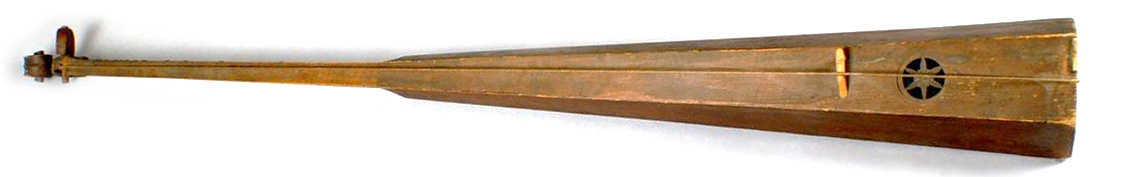
\includegraphics[width=1.0\columnwidth]{figures/trombaHorizontal.jpg}
    \caption{A tromba marina owned by \textit{Nationalmuseet} in Copenhagen, Denmark.}
    \label{fig:trombaHorizontal}
\end{figure}
The tromba marina is a bowed monochord from medieval Europe \cite{encyclopaedia2020} (see Figure \ref{fig:trombaHorizontal}). The string rests on a loose bridge that rattles against the body. This rattling mechanism creates a sound with brass- or trumpet-like qualities. Unlike other bowed string instruments, different frequencies are created by slightly damping the string with a finger of the non-bowing hand as opposed to pressing the string fully against the neck. This interaction at different locations along the string triggers the different harmonics of the open string. Furthermore, the tromba marina is bowed closer to the nut, and the finger determining the frequency is closer to the bridge (below the bow).
As the tromba marina is a rare instrument which can be merely found in museums, very few have the opportunity to play it and discover its interesting timbral possibilities. 
We wish to recreate the feeling of playing this instrument by using physics based  multisensory simulations \cite{pai2005multisensory}.

In the context of musical applications, physics based multisensory simulations have shown some interest in the sound and music computing community. 
As stated in 
\cite{danieau2012enhancing}, the combination of haptics and audio visual content has its own specific challenges worth investigating.
Sile O'Modhrain is one of the pioneers that noticed the tight connection between auditory and haptic feedback and investigated how haptic feedback can improve the playability of virtual instruments \cite{o2001playing}.
At the same time, Charles Nichols developed the vBow, a haptic human computer interface for bowing \cite{nichols2002vbow}.
For several years, researchers from ACROE in Grenoble have developed multisensory instruments based on the mass-spring-system paradigm, with custom-made bowing interfaces \cite{florens1990modeles,luciani2005action}.
Such multisensory simulations have recently been made open source \cite{villeneuve2019mass}.
Haptic feedback has also been combined with digital waveguide models for simulating bowed string interactions \cite{sinclair2009audio}.

Simulating the feeling of string-instrument vibrations is particularly important since it has been shown how vibrations' level can be strongly perceived \cite{askenfelt1992vibration}. 
We use democratized VR technologies controlled by a commercial device called the PHANTOM Omni (or simply Omni) by SenseAble Technologies (now 3D Systems) \cite{phantom}.
The Omni is a six-degrees-of-freedom system providing the tracking and haptic feedback (up to 3.3 N) in our application.
Using the same device, Avanzini and Crosato tested the influence of haptic and auditory cues on perception of material stiffness   \cite{avanzini2006}.
Auditory stimuli were obtained using a physically-based audio model of impact, in which the colliding objects are described as modal resonators that interact through a non-linear impact force \cite{avanzini2004physical}.
Auditory stiffness was varied while haptic stiffness was kept constant. Results show a significant interaction between auditory stiffness and haptic stiffness, the first affecting the perception of the second. Passalenti et. al's also used the Omni to simulate the act of plucking a virtual guitar string \cite{passalenti2019a, passalenti2019b, Fontana2020}.

%We want to emphasize that the visuals are only used for guiding the user, as we are most interested in the haptic feedback and audio.

The goal of this project is to explore the experience of interacting with virtual bowed instrument by using physics based simulations and haptic feedback, together with a visual virtual reality (VR) experience. This effectively makes the implementation a virtual reality musical instrument (VRMI) \cite{Serafin2016}. The tromba marina is used solely as inspiration because it affords itself to being a solid starting point by having only one string. Besides that, the rarity of the instrument ensures that the participants do not have prior experience playing a tromba marina, nullifying possible comparisons between a real instrument and the virtual one. At no point the system was evaluated as an alternative to the real tromba marina. The system (and its evaluation) is targeted towards musicians in order to avoid discouragement frequently encountered when non-musicians interact with musical instruments. It is assumed that musicians acknowledge that mastering any instrument require extended study, therefore it is expected that they will not evaluate this system exclusively based on its difficulty to play.

We start by describing the implementation of the system, both from the hardware and software perspective in Section \ref{sec:implementation}, followed by presenting a study that evaluates the setup in Section \ref{sec:eval}. Section \ref{sec:results} shows the results of the evaluation and Section \ref{sec:discussion} discusses these. Finally, concluding remarks appear in \ref{sec:conclusion}.

\section{Implementation}\label{sec:implementation}
The virtual tromba marina consists of three main components: auditory, visual and haptic feedback, all of which will be elaborated on in this section. For visuals, the Oculus Rift CV1 setup was used \cite{Oculus2020}. The setup consists of a head-mounted display (HMD) and a pair of of wireless controllers that provide tracking information and user input through several buttons and a joystick. A diagram showing the full setup of the system can be found in Figure \ref{fig:systemLayout}. The controls, their mapping to the system and the final setup of the system will also be presented. A video showing the implementation can be found in \cite{Trombavideo2020}.

\subsection{Auditory Feedback}
The audio is generated by a physical model of the tromba marina presented in a companion paper \cite{Willemsen2020}. Some parameters of the model are exposed and can be controlled by the user. These are the velocity, force and position of the bow and the position of the finger inducing the harmonics. The algorithm will not be discussed in detail here, but the mapping to the various parameters of the model will be described in Section \ref{sec:controls}.
\begin{figure}[h]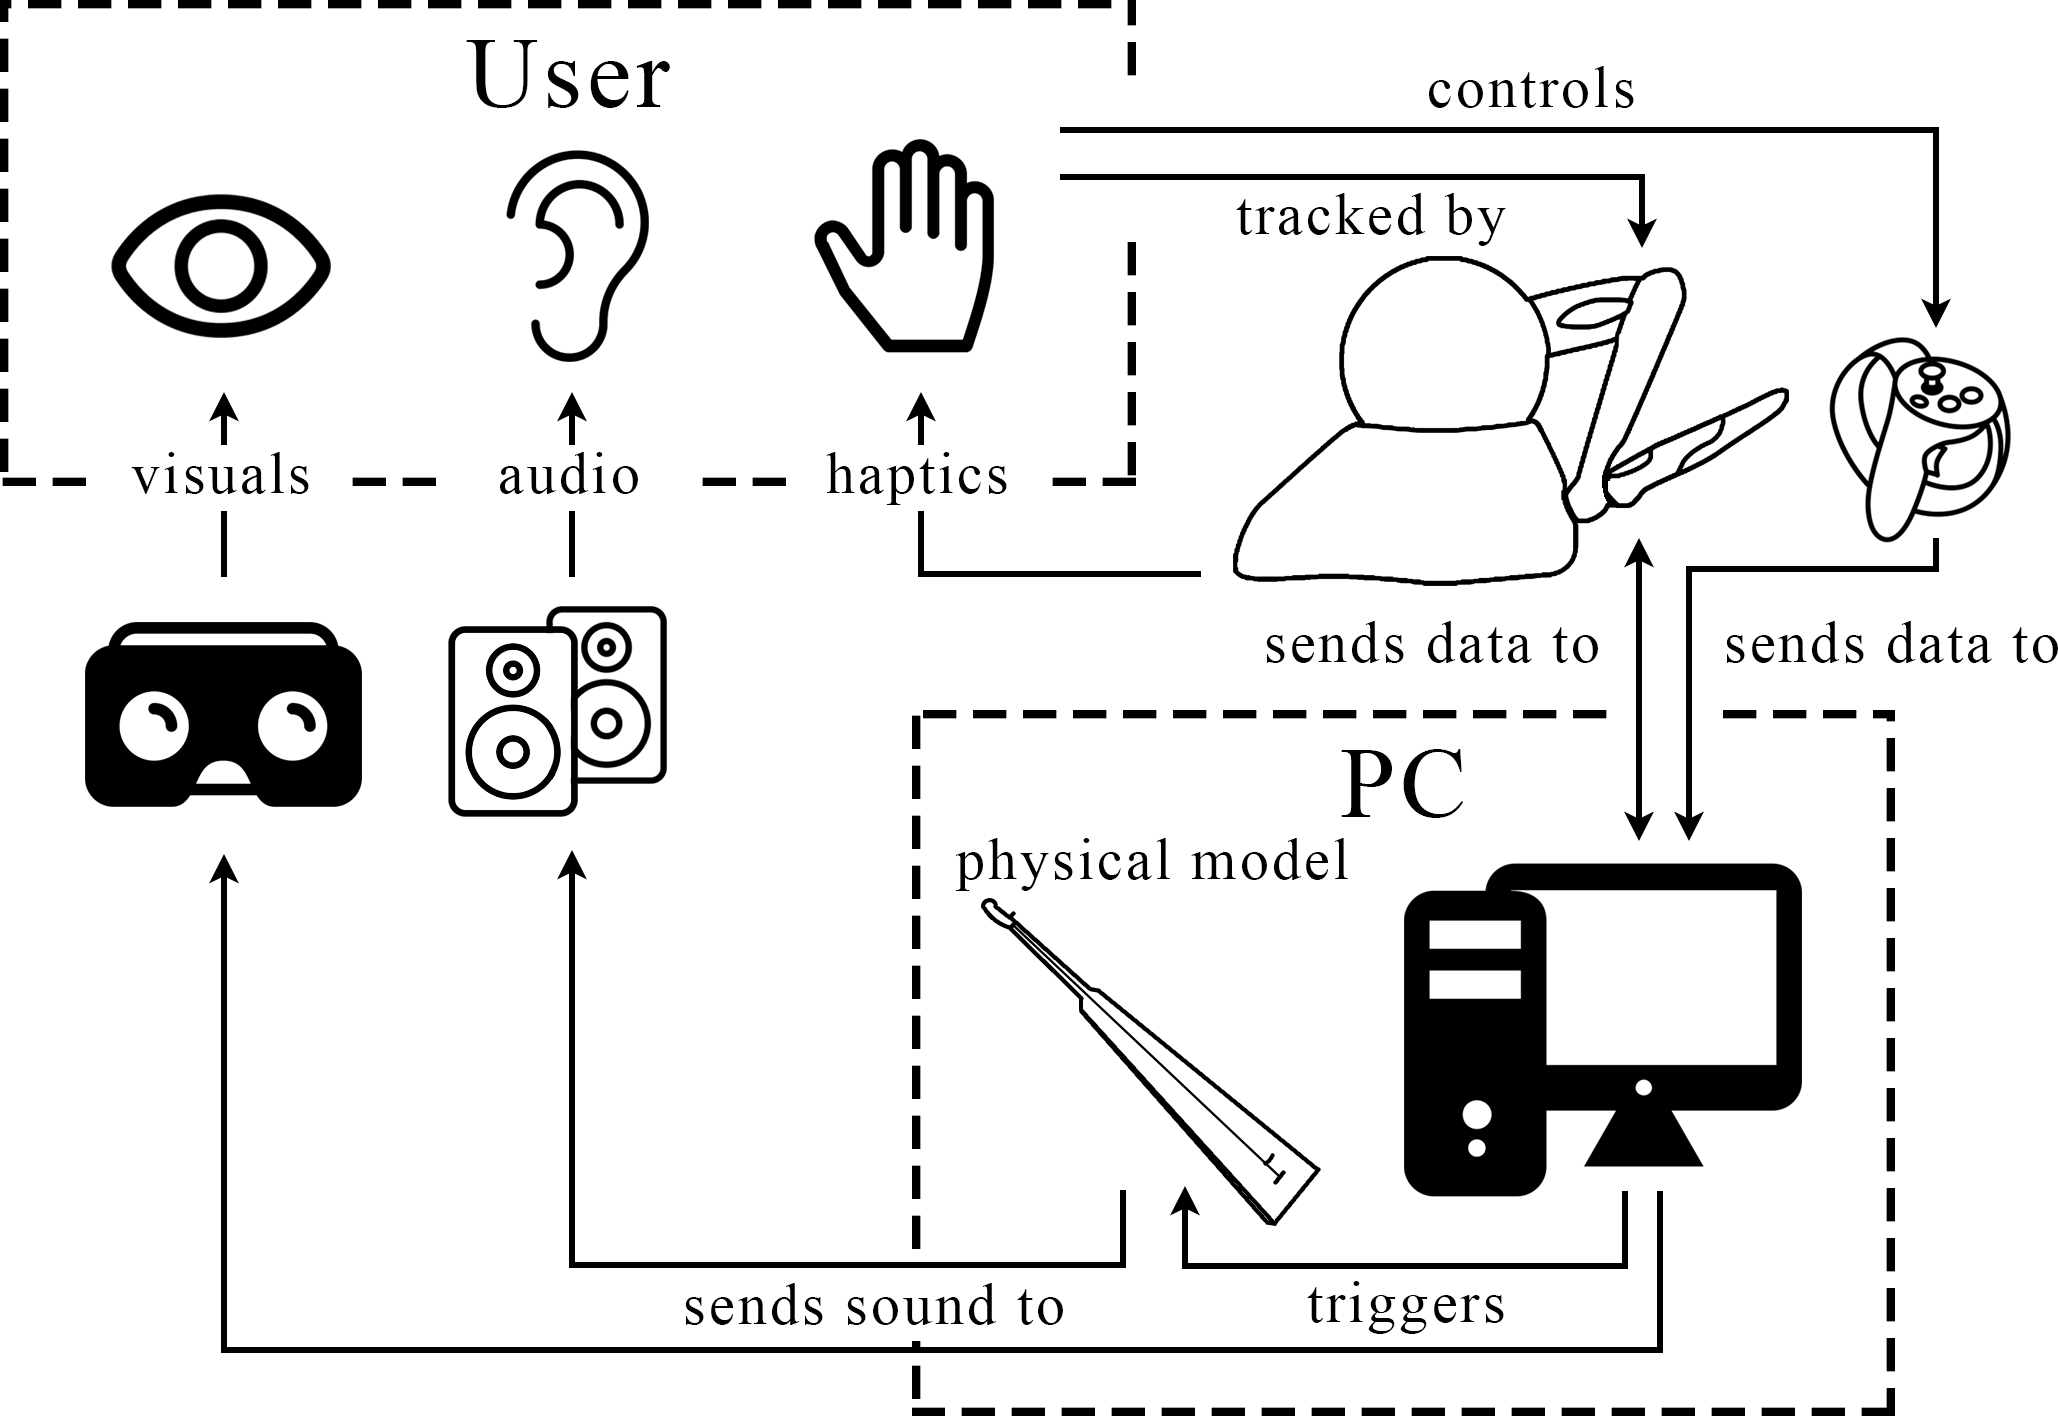
\includegraphics[width=\paperFigWidth\textwidth]{figures/blockdiagram.png}
\centering
    \caption{Diagram showing the system layout of the application. The user interacts with the system using the Omni -- which in turn provides haptic feedback -- and the Oculus Touch controller. These trigger the physical model of the tromba marina. Auditory feedback then comes from speakers and visual feedback from the Oculus Rift headset. A detailed explanation can be found in Section \ref{subsec:physicalSetup}. \label{fig:systemLayout}}
\end{figure}
\subsection{Visual Feedback}
The application was built using the cross-platform game engine Unity3D (or simply Unity) \cite{unity} which can be used to build VR applications. Even though the visual feedback is not the focus of the implementation and eventual evaluation, it was used to guide the users' movements and give them a sense of where the virtual instrument was located. Figure \ref{fig:vrView} shows a screenshot of the view from the HMD, depicting the virtual instrument, the bow and the damping finger indicator. A 3D model of the tromba marina was made inspired by a real-life instrument (presented in \cite{Baldwin2016}) available to the authors. The overall environment resembled a medieval room, providing context to tromba marina's historical nature.

\begin{figure}[ht]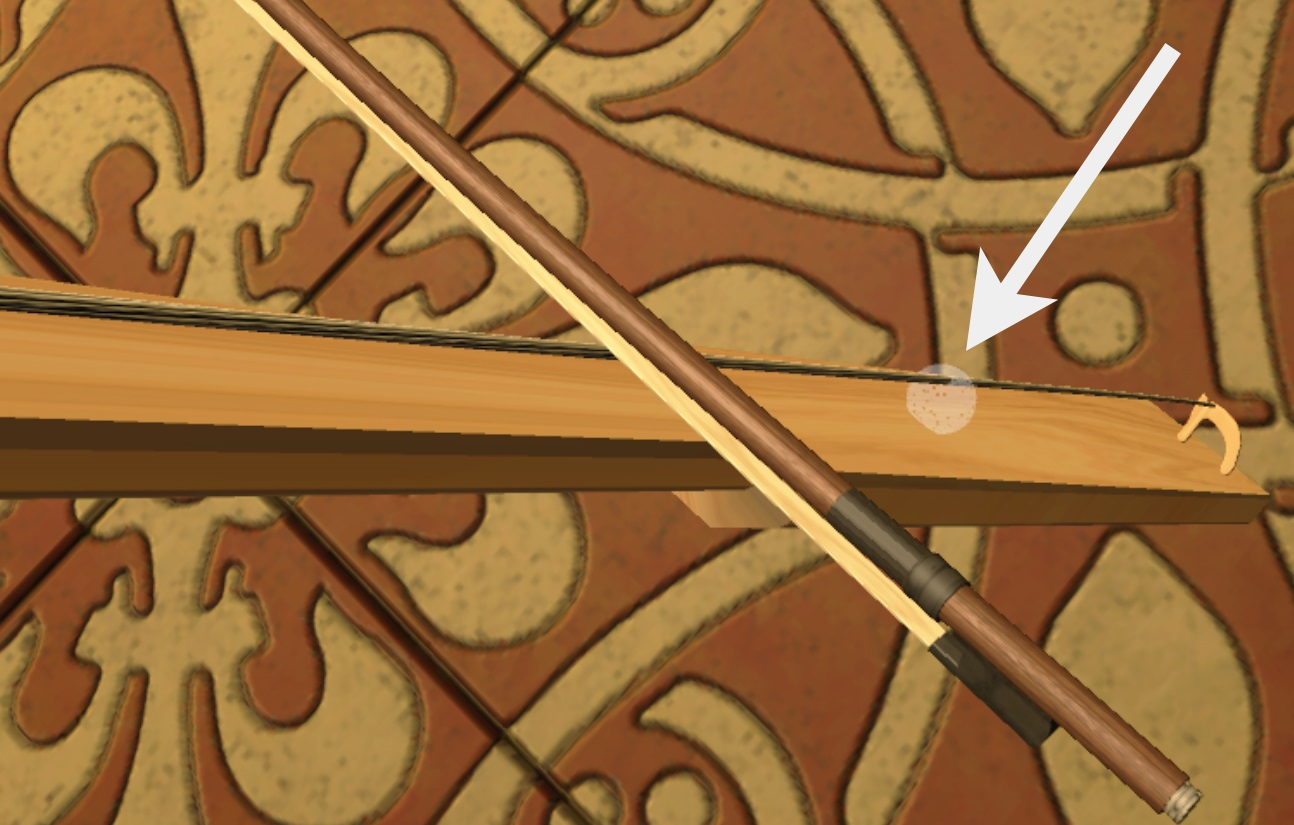
\includegraphics[width=\paperFigWidth\textwidth]{figures/vrView.jpg}
\centering
    \caption{The view from the head-mounted display (HMD). The damping finger is highlighted and shown as a transparent white sphere. \label{fig:vrView}}
\end{figure}

\subsection{Haptic Feedback}
The PHANTOM Omni (or simply Omni) is a six-degrees-of-freedom tracking and haptic system developed by SensAble Technologies (see Figure \ref{fig:omni}). The device has a pen-shaped arm that a user interacts with.  

\begin{figure}[t]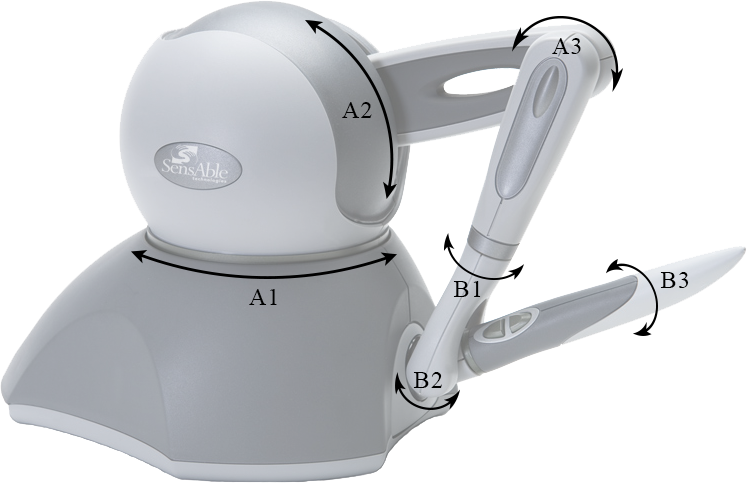
\includegraphics[width=\paperFigWidth\textwidth]{figures/omniSchematic.png}
\centering
    \caption{The PHANTOM Omni has six axes of rotation, three of which provide force feedback (A1-3), and three only tracking position (B1-3). Together, these axes provide six degrees of freedom: x, y and z positions of B2 (according to the shown coordinate system) and rotations of the pen. \label{fig:omni}}
\end{figure}

The raw data provided by the Omni are 1) the absolute position of pivot point B2 (three degrees of freedom), 2) the rotation (three degrees of freedom), and 3) the pressure (touching depth). The latter is calculated from the absolute euclidean distance between the virtual collision point of the object (in our case the bow) and the virtual position of the pen.

The axes are labelled as follows in relation to the virtual tromba marina (also see global coordinate system in Figure \ref{fig:localGlobal}): x-axis (width): horizontally across the soundboard (the common interaction direction), y-axis (height): floor to ceiling, and z-axis (depth): perpendicular to the soundboard. The orientation of the Omni with respect to the aforementioned axis can be seen from the coordinate system in Figure \ref{fig:omni}.

The fact that pivot points B1-3 do not provide force feedback gives rise to an issue in our application. The virtual bow's frog (where it is held by the player) has been placed at the pivot point B2, whereas the interaction between the virtual bow and string happens at an offset as seen in Figure \ref{fig:localGlobal}. To solve this issue, we created a separate game object with which the bow (pivot point B2 to be exact) will interact with in the virtual world Figure \ref{fig:localGlobal}. This `(hidden) collision block' lives in a local coordinate system and its x and y-position exactly follow that of the Omni-pen. The y-rotation will change the rotation of the local coordinate system and uses the virtual string as the center point. If, for any reason, the bow ends up behind the string, the collision block will be offset to the left along the (local) x-axis so that no collision occurs when trying to return the bow to the normal playing area. 

\begin{figure}[t]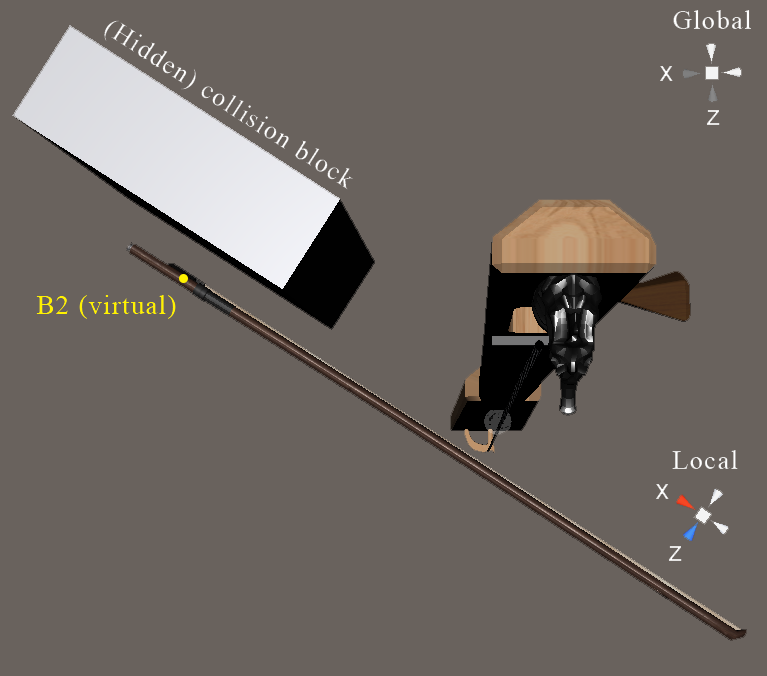
\includegraphics[width=\paperFigWidth\textwidth]{figures/globalLocalUpdated.png}
\centering
    \caption{Top-down view of the global and local coordinate system (x-z--plane). The rotation of the local coordinate system around the (global) y-axis is determined by the y-rotation of the bow. The (normally hidden) collision block lives in the local coordinate system. Its (local) x and y-position follows the (local) x and y-position of B2.\label{fig:localGlobal}}
\end{figure}
Through a list of pseudophysical parameters, the collision forces computed by Unity's physics engine are mapped to the haptic feedback produced by the Omni. Through empirical testing, the following pseudophysical parameters have been found: \textit{Stiffness}: 0.003, \textit{Damping}: 0.0071, \textit{Static Friction}: 0, \textit{Dynamic Friction}: 0.109, and \textit{Pop-through}: 0. For more information, please refer to \cite{OmniAPI2018}.

Throughout implementation, it was considered to actuate the Omni's pen with the output of the physical model used for the auditory feedback, in order to replicate the stick-slip interaction encountered in a real bowing scenario. This was deemed unnecessary, as the Omni's internal gearing systems provide a similar, though uncorrelated, haptic feedback, which satisfied the authors.

% \begin{table}[h]
%     \centering
%     \begin{tabular}{|c|c|}
%     \hline
%         Parameter & Value \\\hline
%         Stiffness & $0.003$ \\
%         Damping & $0.0071$ \\
%         Static Friction & 0 \\
%         Dynamic Friction & 0.109 \\ 
%         Pop-through & 0\\\hline
%     \end{tabular}
%     \caption{Pseudophysical parameters chosen for the haptics.}
%     \label{tab:pseudoParams}
% \end{table}
%
\subsection{Controls and Mapping}\label{sec:controls}
As most people are right-handed, it was chosen to also have the bow in the right hand in the application. The (now-local) x-velocity of the Omni is mapped to the bow velocity, pressure to bow force and y-position (including rotation around the local z-axis) to bow position. The left hand is used to control the pitch by changing the position of the damping finger along the string. This position is defined as
\begin{equation}\label{eq:node}
    x_\text{f} = L\cdot n^{-1},
\end{equation}
%
where $L$ is the length of the string and $n \in [2,8]$. If $n$ is an integer, it is the number of the harmonic we want to induce. The lowest harmonic has been set at half the string length $L/2$, meaning that the string is never completely open. The highest harmonic (8 in this case) has been chosen to be the one that can still be (comfortably) reached. The location of the damping finger $x_\text{f}$ is controlled using the `X' and `Y' buttons and the joystick on the left Oculus Touch controller. % (see Figure \ref{fig:oculusController}). 
The buttons are used for ``discrete harmonic" control of the damping finger, i.e. integer values of $n$ in Equation \eqref{eq:node}, where `Y' increases $n$ and `X' decreases it. The joystick allows for fine pitch control, i.e., decimal values of $n$, and moves the damping finger up and down the string. The latter could potentially create pitch glides in the output sound of the application, but make it harder to `hit' a perfect harmonic according to Equation \eqref{eq:node}. If a button is pressed while the current finger position is between two discrete points, the position will move to the next or previous discrete position, depending on the button pressed.
%As the position of the first node along the string is at \begin{equation}\label{eq:node}
%     x_\text{node} = L\cdot n^{-1},
% \end{equation}
% where $L$ is the length of the string and $n \in [2,8]$ is the harmonic number, we want the damping finger to be set to these positions to induce these harmonics. The lowest harmonic has been set at half the string length $L/2$, meaning that the string is never completely open. The highest harmonic has been chosen to be the one that can still be (comfortably) played. The location of the damping finger ($x_\text{f}$) is controlled using the `X' and `Y' buttons and the joystick on the left Oculus controller (see Figure \ref{fig:oculusController}). The buttons are for discrete control of the damping finger, where `Y' increases $n$ in Equation \eqref{eq:node} and `X' decreases it. The joystick allows for fine pitch control  and moves the damping finger up and down the string. The latter could potentially create pitch glides in the output sound of the application, but make it harder to `hit' a perfect harmonic according to Equation \eqref{eq:node}. If a button is pressed while the current finger position is between two discrete points, the position will move to the next or previous discrete position, depending on the button pressed.

% \begin{figure}[ht]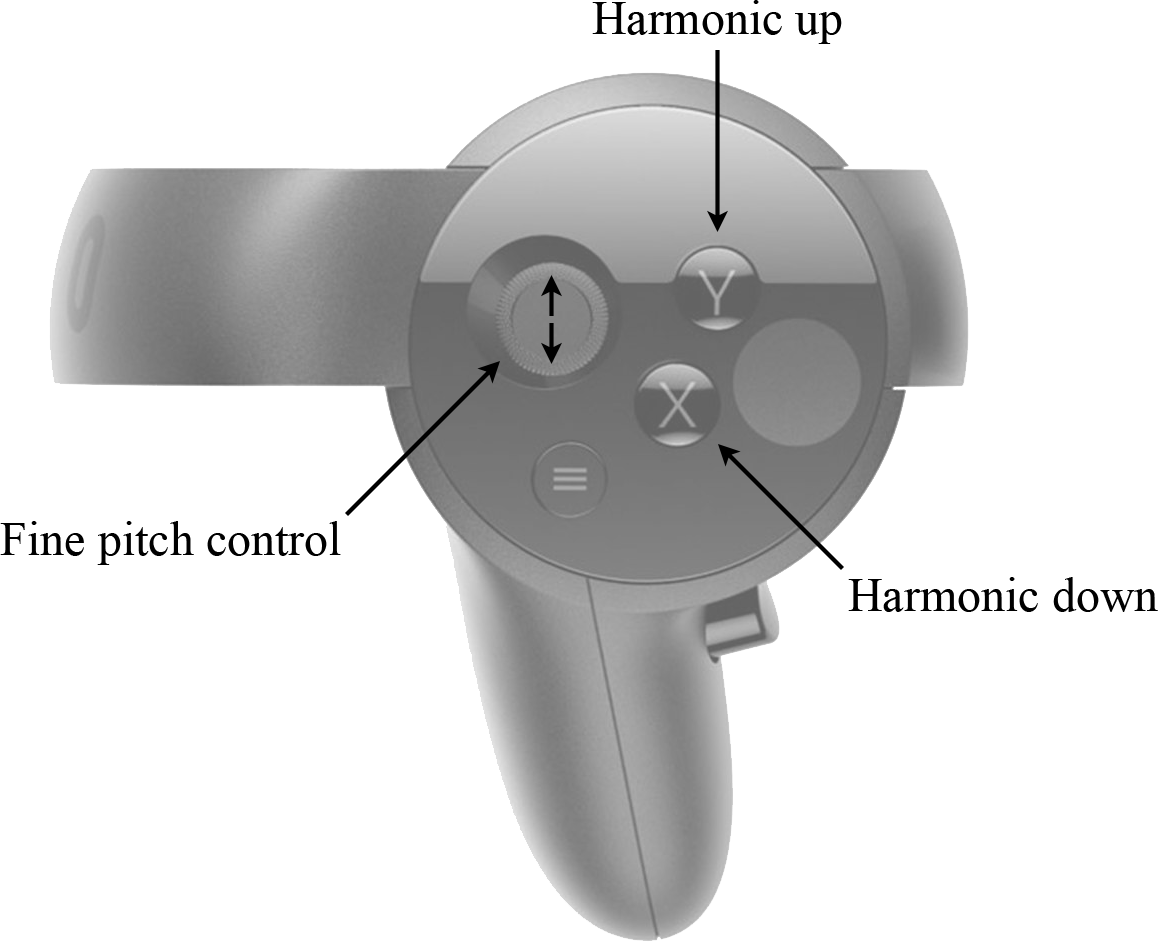
\includegraphics[width=1.0\columnwidth]{figures/controller.png}
% \centering
%   \caption{The left Oculus Touch controller. The controls for changing the pitch are highlighted. \label{fig:oculusController}}
% \end{figure}
\subsection{Physical Setup}\label{subsec:physicalSetup}
The physical setup is shown in Figure \ref{fig:physicalSetup}. The Omni is mounted on a stand at \textapprox125 cm to match the approximate bowing height of the real instrument. As can be seen in Figure \ref{fig:physicalSetup}, the right Oculus Touch controller is mounted right underneath the Omni. This is used to align the physical setup with the virtual tromba marina, both in the x-z--plane but also the height of the bow in the application. After the scene is initialised the controller is used for a tilting interaction so that the instrument can rest on the user's body, as is done with the real instrument. The aforementioned alignment came with a drawback -- as the center of the x-axis range of the Omni was aligned with the tromba marina and B2 was aligned with one end of the bow, only half of the range of the Omni could be used for bowing.

% \begin{figure}[ht]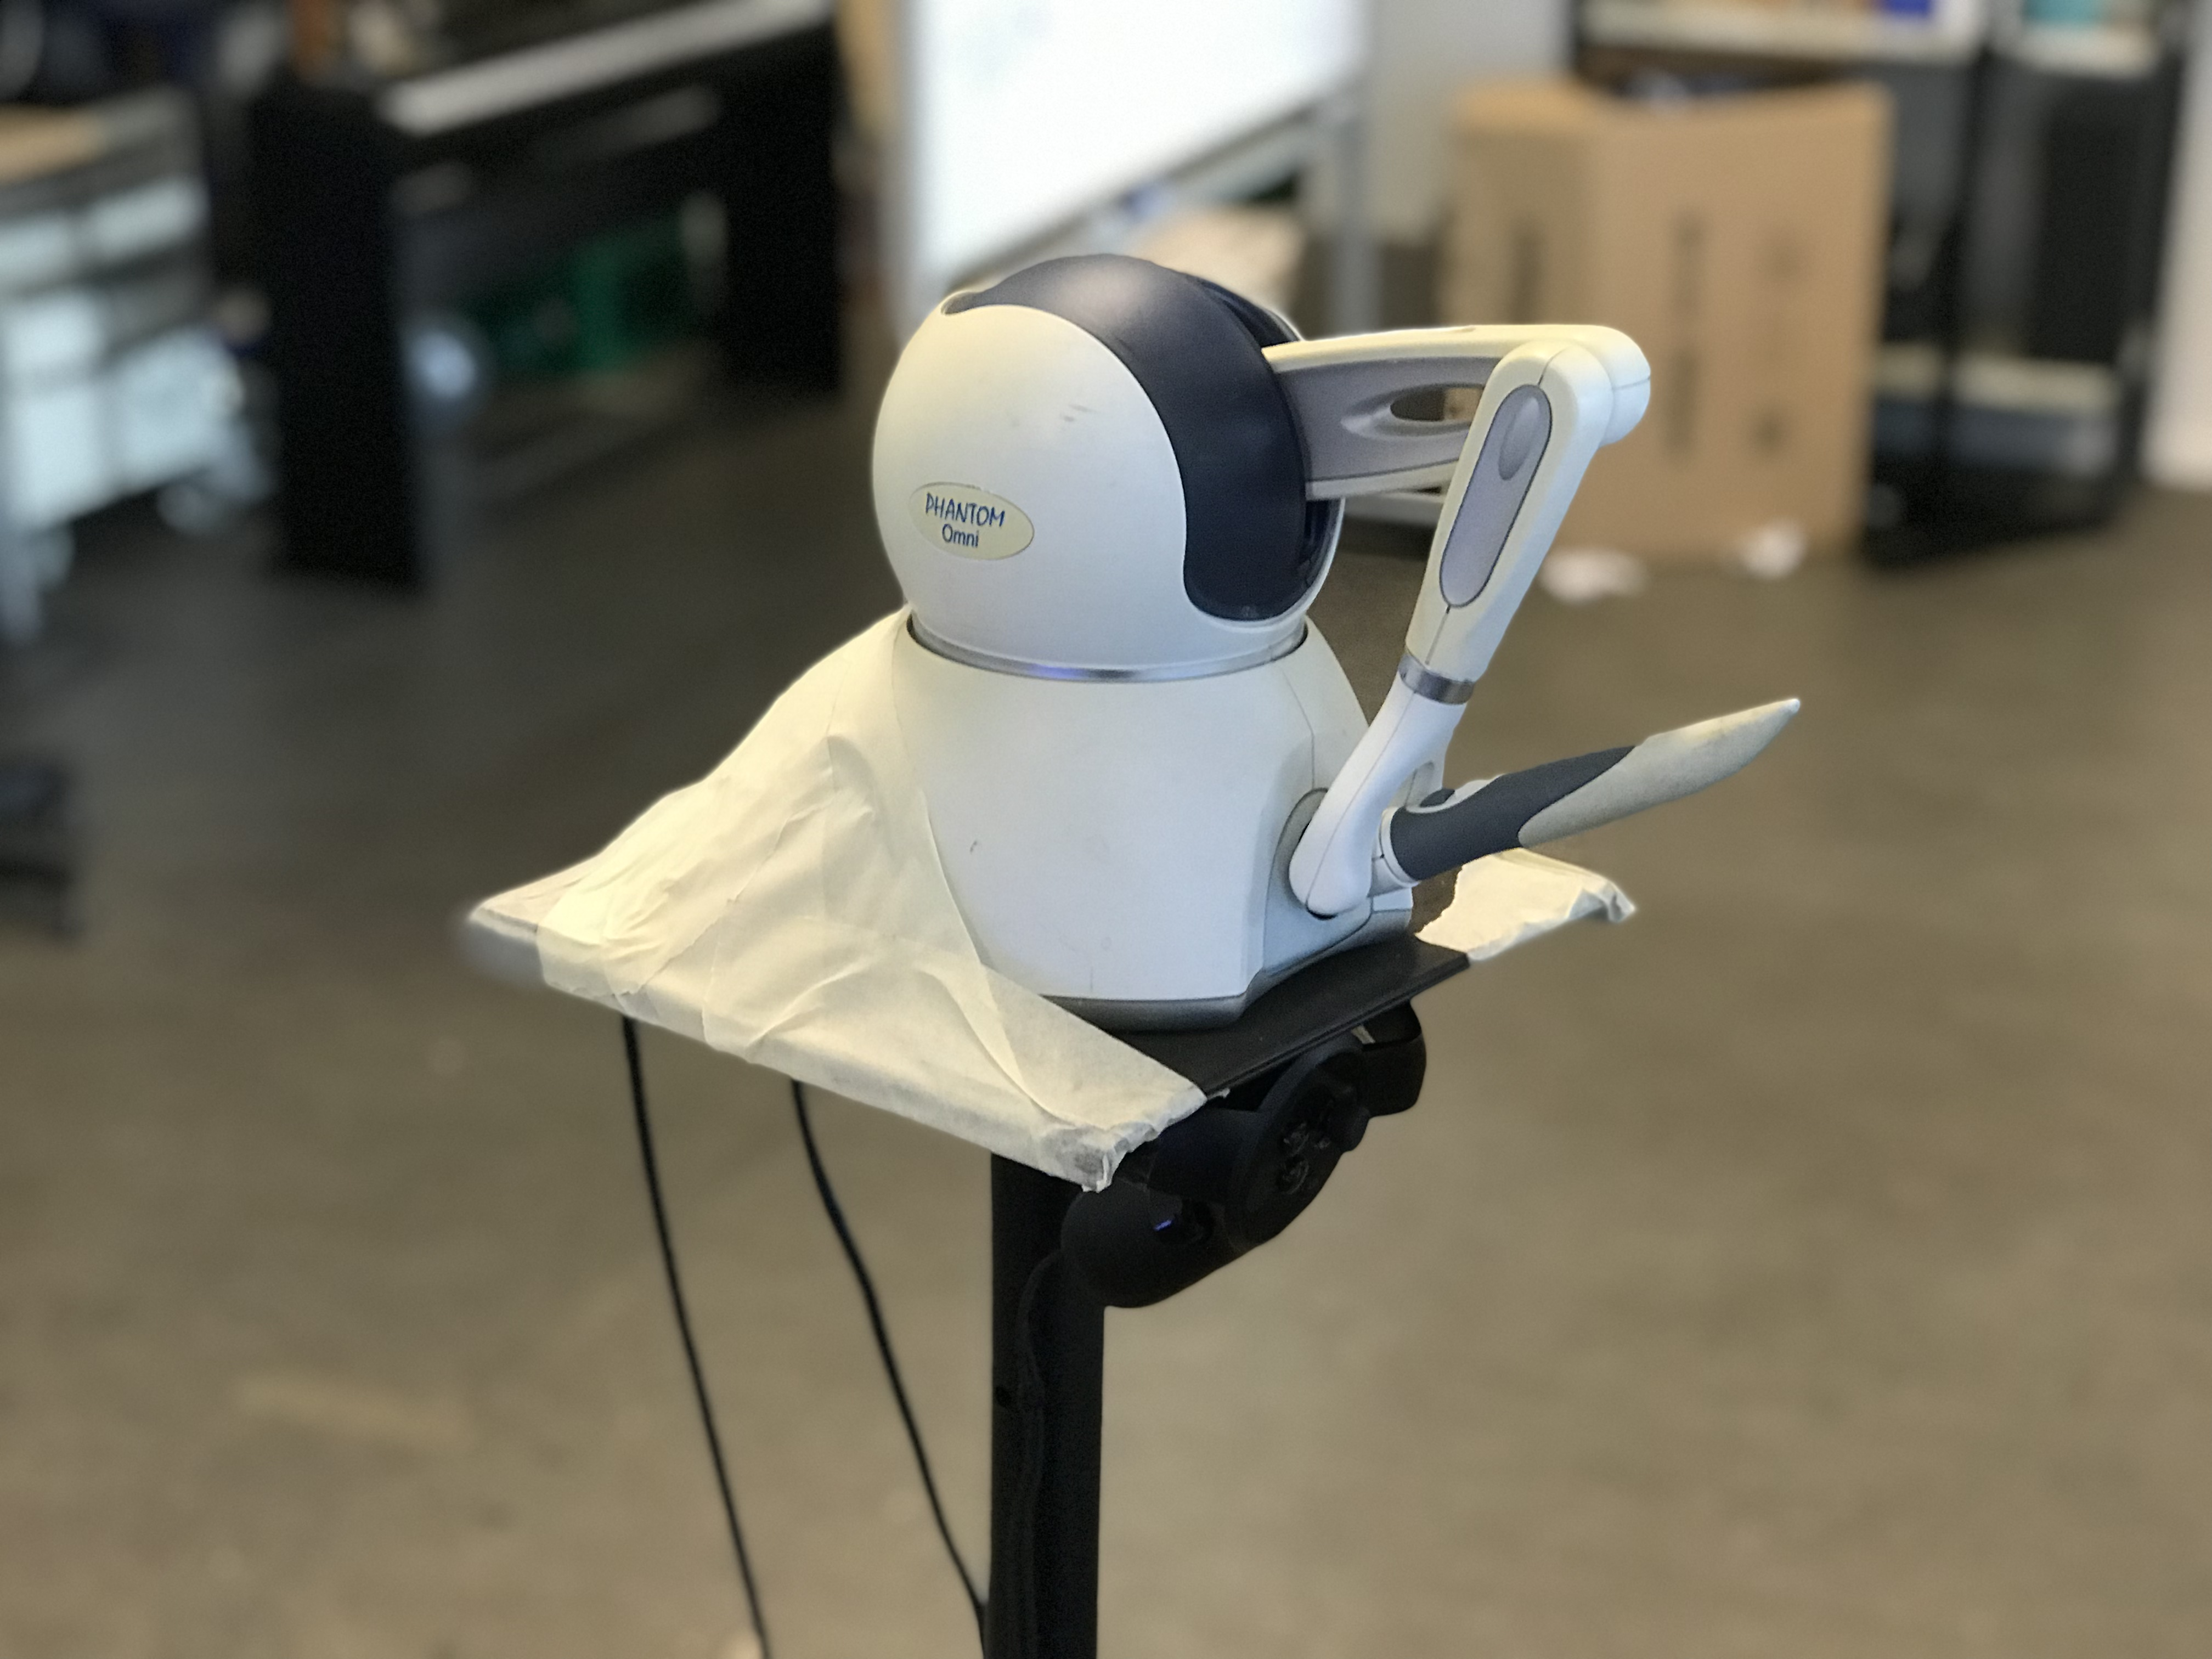
\includegraphics[width=1.0\columnwidth]{figures/omni.jpg}
% \centering
%   \caption{Diagram showing the system layout of the application. The user interacts with the system using the Omni -- which in turn provides haptic feedback -- and the Oculus Touch controller. These trigger the physical model of the tromba marina. Auditory feedback then comes from speakers and visual feedback from the Oculus Rift headset. A detailed explanation can be found in Section \ref{subsec:physicalSetup}. \label{fig:systemLayout}}
% \end{figure}

\begin{figure}[t]\includegraphics[width=\paperFigWidth\textwidth]{figures/Cumhur.jpg}
\centering
    \caption{User interacting with the physical setup. The Omni is mounted on a \textapprox125cm stand together with the right Oculus Touch controller used for location and tilting information. \label{fig:physicalSetup}}
\end{figure}
The setup shown in Figure \ref{fig:systemLayout} is implemented as follows: the user controls the application using the Omni (for tracking) and the left Oculus Touch controller which sends data to the computer running the application. The Omni produces haptic feedback based on Unity's physics engine calculating the interaction force between  the `(hidden) collision block'  and the virtual bow as shown in Figure \ref{fig:localGlobal}. This data simultaneously triggers the physical model which sends its output to a pair of speakers. The user wears a HMD that gives visual information about the location of the tromba marina (and medieval scene). The user's position in the VR environment is controlled by the HMD, but this dataflow is not visualised in the diagram. Lastly, the right Oculus Touch controller is attached to the stand the Omni is attached to, and sends position and tilting data to the application.



\section{Evaluation}\label{sec:eval}

The goal of the study was to (1) evaluate the  general experience of bowing in a VR environment using haptic feedback and accurate physical modelling and (2) to evaluate the  playability of a VR monochord instrument. This was done by exploring the quality of the software, the acoustic model, the interface and the mapping, as proposed by \cite{Barbosa2015} and implemented previously in a similar study \cite{Young2003}. To meet this aim, an investigative study was performed through which feedback on the virtual instrument was collected. In order to ensure a high level of validity and reliability, a triangulation of methods has been used: think aloud protocol \cite{Someren1994} throughout the interaction, observation and post-study self report through a modified Usability Metric for User Experience survey \cite{Finstad2010}. The study concluded with an semi-structured interview based on the observed actions, noted comments and questions loosely revolving around \textit{goals, operators, methods and selection} method \cite{Card1983}.

\subsection{Participants}

A total of 14 people (12 male, 2 female), 23-48 years old (M=29.5, SD=7.65)  participated in the study. All participants were students or staff at Aalborg University Copenhagen. The selection of participants was based on the single criterion that one had to have experience playing a musical instrument. Over 70\% of the participants have been playing an instrument for more than 5 years, guitar being the most common occurrence (25\%). There was only one participant experienced in playing bowed instruments (violin). The same participant mentioned playing the tromba marina briefly before, but the majority of the other participants had never heard (of) it. All but one participant have had tried VR experiences before joining the study. 

\subsection{Procedure and Task}

The experiment started with the participant reading an introduction about the experiment and completing a questionnaire covering several demographic questions (age, gender, musical experience, familiarity with the tromba marina and VR experience). They were then introduced to the setup and task, and controls were explained. The participants were informed that the study is exploring the experience of bowing in a VR environment. It was emphasised that the most important part of the experiment was for the participant to talk aloud with the phrase: ``anything positive, negative, basically anything that comes to mind, please speak out loud". Furthermore, the user was instructed to bow above the damping finger (visualised as a white sphere) at all times, as this is also the interaction with the real instrument. 

The interaction part was divided into two phases. Firstly, the participants were asked to freely explore the instrument on their own. Then, when they felt they are ready to move on, an audio recording made by the authors using the application was played, showcasing the system's capabilities, aiming to inspire the second phase of free exploration. It was stressed that the participants did not have to recreate what they heard, but to merely use it as inspiration. The experiment concluded with participants completing a questionnaire covering usability and playability of the system. Finally, a semi-structured interview was held which lasted 5 minutes on average. 

Throughout the interaction phase, the participants' actions were observed and noted by the authors, and their comments written down. Most participants were encouraged again to think aloud during their exploration. The full experiment lasted \textapprox30 minutes for all participants.
\subsection{Measurements}

Because the  goal of the study was to investigate the overall experience of bowing in VR, as well as evaluate the playability of the instrument,  self-reporting measurements were used in combination with the observations, interview and \textit{think aloud} notations. Specifically, after exposed to the instrument, the participants were asked to fill out a questionnaire containing 20 items related to the experience of interacting with the VRMI. The items can be broadly segmented into four categories: overall experience, haptic feedback, auditory feedback and visual feedback. Table \ref{tab:questions} presents the questions.

\begin{table}[h]
\centering
    \small
    \begin{tabular}{p{0.95\columnwidth}}
    \textbf{Questionnaire items:} \\
    \hline
    \\[-0.1in]
    \textit{Overall experience:} \\
    (1) It was easy to understand how to play the instrument.\\
    (2) I felt the instrument was hard to play.\\
    (3) I felt the instrument was expressive.\\
    (4) The instrument's capabilities did not match my expectations.\\
    (5) I felt I could easily achieve my goals.\\
    (6) I made many errors playing the instrument.\\
    (7) I am satisfied with the instrument.\\
    (8) I felt the instrument was boring.\\
    (9) Interacting with the instrument was frustrating.\\
    \hline
    \\[-0.1in]
    \textit{Haptic feedback:}  \\
    (10) I felt the haptic feedback was realistic.\\
    (11) I felt the haptic feedback was too strong.\\
    (12) I felt the haptic feedback was natural.\\
    \hline
    \\[-0.1in]
    \textit{Auditory feedback:}\\
    (13) I felt I was in control of the sound.\\
    (14) I felt the audio was matching my actions.\\
    (15) I felt the sound was matching the haptic feedback.\\
    (16) I felt the sound was matching the visuals.\\ 
    (17) I felt the sound was static.\\ 
    \hline
    \\[-0.1in]
    \textit{Visual feedback:}\\
    (18) I felt the visual feedback was helping me play.\\
    (19) I felt the visuals were confusing.\\
    (20) I felt the visuals were matching my actions.\\
    
    \hline
    \end{tabular}%
        \caption{The questionnaire items and corresponding anchors of the 5 point (1 -- 5) rating scales (Strongly disagree -- Strongly agree).}
    \label{tab:questions}
\end{table}
%
\section{Results}\label{sec:results}
This section presents the results obtained from the self-reported measure regarding the participants' experience as well as the qualitative findings from interview, observations and think aloud.

\subsection{Quantitative Data}
The data obtained for the questionnaire items was treated as ordinal and analysed in terms of central tendency (medians and mode), interquartile ranges, minimum and maximum ratings. Figure \ref{fig:boxplots} visualises the collected data. The mode was considered only when different from the median, specifically question 8, 13 and 14. It is worth noting that most of the items show a skewed normal distribution.

Question 1-9 paint a picture of how the instrument was perceived by the users. Questions 1, 2, 4, 5, 6 and 9 cover the perceived difficulty of using the system as a musical instrument. The answers to these questions show that even though participants generally found the instrument easy to understand, they had difficulty playing it and reaching their goals.
Questions 3, 7 and 8 cover their general opinion about the instrument. Participants generally felt satisfied and not bored with the instrument.
Questions 10-12 cover exclusively the impressions about haptic feedback. It can be seen that most participants found the haptic feedback to be realistic and generally natural and the force to be not too strong.
The questions 13-17 approach the auditory aspect of the instrument, focusing on its perceived characteristics. As can be seen from questions 13, 14 and 17, the participants felt a high level of command over the sound, and were satisfied with mapping between the haptic and auditory feedback. The same thing can be said about the visual mapping, as indicated by question 16. 
Items 18-20 investigate the perceived visual quality. It can be seen that the visuals helped the participants play and were implemented well, i.e., not confusing and matching their actions.

\begin{figure*}[!t]
    \centering
    \includegraphics[width=1.0\textwidth]{figures/Boxplots.jpg}
    \caption{Boxplots visualizing the results related to the 20 questionnaire items (shown in Table \ref{tab:questions}) in terms of medians (red lines), interquartile ranges (blue rectangles), minimum and maximum ratings (dashed lines), and outliers (red crosses). The y-axis maps "Strongly disagree -- Strongly agree" to a 1 -- 5 interval.}
    \label{fig:boxplots}
\end{figure*}

\subsection{Qualitative Data}
In order to present an accurate representation of the findings, this section will be split into two categories: actions -- covering the observed activities during the interaction phase, and oral feedback -- presenting the findings from the think aloud protocol and interviews.

\subsubsection{Observed Actions}
Since there were no tasks given to the participants, all actions were noted and analysed. That said, most users performed similar actions in their interaction phase. All participants experimented with bowing at different heights, but only a few of them tried to explore bowing heights for all discrete pitches. Most of them were satisfied with trying different heights on whatever pitch they found themselves at that time. In a similar fashion, all participants experimented with playing different pitches, both using the discrete buttons as well as the joystick. It is worth mentioning that many users tried to investigate the limits of the pitches they could play. Higher pitches usually resulted in little or no sound which was commented on by most. This behaviour is true to a real tromba marina, where higher harmonics are harder to excite than lower ones. The majority tried to perform some form of glissando, as well as bowing with different velocities, usually commenting on the findings. Due to the non-intrusive nature of observation, it was impossible to notice the pressure applied with the bow, but some participants explicitly mentioned that they tried to experiment with different forces. This was especially true in the second phase of interaction, when they experimented with a higher dynamic range of sounds. Another common occurrence was the attempt to play some sort of melody or riff. Simple melodies like \textit{Mary had a little lamb}, or \textit{Twinkle twinkle little star} were attempted, with various degrees of success. One participant tried to play a Mozart segment. The last commonality was found in the attempt to perform a sustained tone, with a constant bowing speed and a back-and-forth motion.

When it comes to seldom or individual actions, a great variance in experimentation was observed. Participants tried to hit the string with the bow, rotate the bow upwards to the point of it being parallel to the string, move the bow in an up-down (y-axis) motion, bow on the damping finger indicator and underneath it or play some form of vibrato or staccato. No one tried to tilt the stand supporting the Omni.

\subsubsection{Oral Feedback}

Generally the overall impression of the instrument was positive, described with words like: \textit{cool, fun, interesting, weird}, as well as \textit{hard} or \textit{difficult to play}. One participant's answer encapsulates this very well by saying: ``I got to express my ideas, but not perfect them". 

Just as described in the previous section, there was a general consensus on several reported characteristics. All participants that attempted to play the highest harmonic said it is hard to play, and that it felt frustrating. At the other end, several participants expressed their preference towards lower pitches, where some said that they prefer the sound produced when bowing under the damping finger (essentially playing the lower-pitched open string). Besides that, many reported that is was hard to maintain a sustained tone, regardless of the pitch. Another sound-related report was the inability to re-create the buzzing sound heard in the recording; one of the participants familiar with the tromba marina's mechanism even mentioned specifically that he ``couldn't get the bridge to rattle". When it comes to the pitch selection interface, the reports are very polarised between the joystick and the buttons. On one hand some describe the buttons as being more, \textit{fun, musical, melodic, useful} or \textit{easier}, while describing the joystick as \textit{useless, unrealistic, too hard} or \textit{meaningless}. On the other hand some participants clearly preferred the joystick describing it as \textit{natural, intuitive, interesting, expressive} or \textit{humane}, but everyone mentioned that the sensitivity of the joystick is too high, making it hard to land on the desired pitches. Due to the incremental nature of the damping fingers' position, it was impossible to skip over notes, a fact that was mentioned in different forms by several participants. Some noted that the control of the damping finger (`Y' for up the string and `X' for down) should have been inverted. Furthermore, some would have liked a more physical interaction for the damping finger, such as moving the controller up and down rather than using buttons.

When it comes to the haptic feedback, the majority was satisfied with it, mentioning that ``it feels nice", ``it feels good", ``is great", ``impressive - it felt natural", or ``it feels real", while one participant found it to be ``wild and a bit too powerful". A special case related to the haptic feedback was the bounce obtained by hitting the virtual string with the bow. Most subjects found it pleasing and were intrigued by its realistic feel, but the violin player repeatedly mentioned that it is ``unrealistic and way to powerful". One participant explicitly mentioned that the haptic feedback matches the auditory one, and his expectations.

Several participants noticed that the bow could rotate along its axis and asked whether it made a sonic difference or not, to which they were answered negatively. Besides that, there were very few comments regarding the visual aspect of the system, but most of these were positive. One participant mentioned that sometimes there's a gap between the string and the bow, and that it would be nice to observe one's hands.  No one mentioned anything related to the visual indication or the damping finger seen in Figure \ref{fig:vrView}.

The overall interaction was described offering a high degree of freedom on the bowing hand, but the pitch selecting hand was either not mentioned, or described as \textit{disconnected} several times. Some agreed that the instrument is hard to play, mentioning that it is \textit{frustrating}. However, most people estimated that they can perform better after practising more.

% \begin{figure}[ht]\includegraphics[width=1.0\columnwidth]{figures/PlayabilityChart.pdf}
% \centering
%   \caption{Playability chart of a virtual musical instrument \cite{Young2003}. \label{fig:oculusController}}
% \end{figure}

\section{Discussion}\label{sec:discussion}

\ifx
%############################
To cover in discussion chapter
#1. think aloud protocol might be bad 
#2. Example sound - some tried to do replicate but they couldn't - might have influenced the goal question
#3. Bounciness was regarded as really cool and realistic, even though it's more of a byproduct
#4. Bow length and passing through the string - Silvinging
#6. Miss alignment between bow initial position and haptic omni pen - Haptic omni has a gained/exaggerated motion mapping
#7. highest pitch it's hard to excite
#8. joystick is to sensitive, some hate it, some love it
#9. pitch range, and playing below the string
10. no one use the tilting?! p.s. we forgot to mention that we used Peter to help us design. 
11. talk about why the left hand is static

%############################
\fi

%Recalling our goal (at the beginning of Section \ref{sec:eval}) 
In this section, both the evaluation procedure itself and the results from Section \ref{sec:results} will be discussed.

\subsection{Procedure}
It is acknowledged that the cognitive load of speech and playing an instrument are overlapping \cite{Stowell2009}, therefore the \textit{think aloud protocol} might have not generated in the most abundant data possible. Most participants alternated between playing and speaking. This resulted in occasionally long breaks in either activities, and required participants to be encouraged to think aloud. Retrospectively, a structured activity schedule allocating time for playing and feedback could have been more productive. Similarly, using self report through Likert scales require large sample sizes to achieve a high level of accuracy\cite{Stowell2009}. Therefore the interpretation of results rooted into the qualitative data, and then validated using the quantitative data. 

Furthermore, as the data we obtained was purely through non-intrusive methods, it would have been useful to log the raw data provided by the Omni (such as the bowing pressure). This could then have been analysed to obtain a better understanding of the user's feedback.

Lastly, the audio did not fully match the sounds that were possible to create with the application. As the recording was quite distorted, the volume of the audio plugin was turned down during the test, but the recording was not remade. This will be elaborated on below.

\subsection{User Feedback}
The generally positive oral feedback about the overall experience is backed up by the quantitative data which showed that participants were satisfied and not bored with the instrument. They attempted to perform fundamental tasks as producing a sustained tone or playing simple melodies with various degrees of success, and when exposed to the example recording, some tried to recreate the sounds heard from the audio clip. Several participants mentioned that it was difficult to achieve this particular goal, a problem that finds its explanation in the difference in volume between the recording and the experiment scenario as mentioned above. This would be a point of improvement for future testing, as it could have impacted the answers for question 5 -- the lowest scoring question regarding the overall experience. Another reason for this question's answers could be linked to the inability to play the higher notes, or the limited pitch range, as presented in Section \ref{sec:results}, but these characteristics are inherited from the physical characteristics of the real instrument, so could be expected.

Interestingly, many participants believed that it was easy to understand how to play the instrument, but that they could become better after some more practice. %This can also be seen from the participants' answers to the questions covering perceived difficulty. 
This indicates that the setup has a low ``entry-level", with an envisioned high virtuosity ceiling. This is believed something desirable when creating computer based instruments \cite{Wessel2002}. Even though the implementation was inspired by a real instrument with a possibly different learning curve, as mentioned, it was not our goal to recreate it.  

The haptic feedback was considered positive and generally having an appropriate level of resistance to movements. The answers to questions 10 (realistic haptic feedback) and 12 (natural haptic feedback) correlate positively and question 15 (sound matching the haptic feedback) was also answered positively, giving a strong indication that the participants considered the haptic feedback real and according to their expectations.  It can be understood that the realism of the haptic feedback is estimated considering the multisensory experience and this result reassures that bowing in VR with our setup is possible.

Furthermore, many participants noticed that they could `bounce' the bow onto the string. Even though this behaviour was a byproduct of the implementation, participants generally liked this interaction and found it to be realistic and exciting.  

Many users noted that the full range of the bow could not be used. As mentioned in Section \ref{subsec:physicalSetup}, the virtual tromba marina was aligned with the physical position of the Omni and as the bow is held at one end, about half of the range could not be used for bowing. This was a commonly reported issue, and it could have impacted the answers for questions 4, 5, and 9. The reason for aligning the physical setup with the virtual tromba marina was the tilting interaction, so that if people wanted to interact with the entire instrument, they would be able to grab the physical setup. As none of the participants used this, we could discard the aforementioned alignment to be able to account for the entire range of the bow. %This was done in an attempt to compensate for the inconsistency between the movements of the bow in the real world, and the virtual world. This inconsistency was due to the fact that the Phantom Omni's Unity3D plugin applies an unknown gain coefficient to translation motions.  

The polarisation of the participants' opinion on the pitch control -- joystick versus buttons -- was backed up by the answers individuals gave on question 9 (interaction was frustrating). It could be argued that users preferring the joystick over the buttons had a harder time interacting with the instrument than the people preferring the buttons. As mentioned, all participants who mentioned the joystick interaction said it was too fast, explaining the above.

\section{Conclusions} \label{sec:conclusion}
This paper presents a virtual reality implementation of the tromba marina and its evaluation. Our goal was to evaluate the general experience of bowing in VR and to evaluate the playability of our implementation. The results show that the implementation was successful with participants finding the haptic feedback realistic and the general experience enjoyable and interesting on one hand, and difficult and frequently frustrating on the other hand. Nevertheless, all sensory modalities we focused on (auditory, haptic and visual) seemed to reinforce each other, inspiring participants to attempt to play melodies with the instrument. This was considered to be an important achievement.
Improvements on our application include the pitch control, which  should either be more physical, i.e., moving the pitch hand physically up and down the virtual string, or simply slower continuous control. Besides that, a better physical setup, allowing the users to utilise the entire bow is desired.
The findings of this paper prove that it is possible to create a satisfactory bowed VRMI using off-the-shelf hardware and accurate physical modelling. 

\subsection*{Acknowledgments}
We would like to thank Peter Williams for his valuable insights on playing the tromba marina, feedback on our application and providing access to his instrument replica. 

This work is supported by NordForsk's Nordic
University Hub Nordic Sound and Music Computing Network
NordicSMC, project number 86892.

% \defaultbib
\pagestyle{empty} %disable headers and footers

\makeatletter
\renewenvironment{thebibliography}[1]
     {\section{\bibname}%
      \@mkboth{\MakeUppercase\bibname}{\MakeUppercase\bibname}%
      \list{\@biblabel{\@arabic\c@enumiv}}%
           {\settowidth\labelwidth{\@biblabel{#1}}%
            \leftmargin\labelwidth
            \advance\leftmargin\labelsep
            \@openbib@code
            \usecounter{enumiv}%
            \let\p@enumiv\@empty
            \renewcommand\theenumiv{\@arabic\c@enumiv}}%
      \sloppy
      \clubpenalty4000
      \@clubpenalty \clubpenalty
      \widowpenalty4000%
      \sfcode`\.\@m}
     {\def\@noitemerr
       {\@latex@warning{Empty `thebibliography' environment}}%
      \endlist}
\makeatother

\bibliographystyle{IEEEtran} 
\bibliography{bib/paperA}

\end{document}




% \chapter{Real-Time Control of Large-Scale Modular Physical Models using the Sensel Morph}\label{paper:A}
%frontmatter
\pagestyle{plain} %disable headers and footers
\input{papers/paperA/frontPage.tex}
\ifpapers
    \includepdf[pages=-, pagecommand={}]{papers/paperA/paperA.pdf}
\fi
\pagestyle{plain} %disable headers and footers
\pdfbookmark[0]{Front page}{label:frontpage}%
\begin{titlepage}
  \addtolength{\hoffset}{0.5\evensidemargin-0.5\oddsidemargin} %set equal margins on the frontpage - remove this line if you want default margins
  \noindent%
  \begin{tabular}{@{}p{\textwidth}@{}}
    \toprule[2pt]
    \midrule
    \vspace{0.2cm}
    \begin{center}
      {\fontsize{23pt}{24pt}\selectfont\textbf{
      The Emulated Ensemble}}\\
      \vspace{0.5cm}\Large{Real-Time Simulation of Musical Instruments using Finite-Difference Time-Domain Methods}
    \end{center}
    \vspace{0.2cm}\\
    \midrule
    \toprule[2pt]
  \end{tabular}
  \vspace{4 cm}
  \begin{center}
    {\large
      Ph.D. Dissertation%Insert document type (e.g., Project Report)
    }\\
    \vspace{0.2cm}
    {\Large
      Silvin Willemsen%Insert your group name or real names here
    }
  \end{center}
  \vfill
  \begin{center}
  Dissertation submitted \today
  \end{center}
\end{titlepage}
\clearpage

\ifpapers
    \includepdf[pages=-, pagecommand={}]{papers/paperB/paperB.pdf}
\fi

% \pagestyle{plain} %disable headers and footers
\input{papers/paperC/frontPage.tex}
\ifpapers
    \includepdf[pages=-, pagecommand={}]{papers/paperC/paperC.pdf}
\fi

% \pagestyle{plain} %disable headers and footers
\input{papers/paperD/frontPage.tex}
\ifpapers
    \includepdf[pages=-, pagecommand={}]{papers/paperD/paperD.pdf}
\fi

% \pagestyle{plain} %disable headers and footers
\input{papers/paperE/frontPage.tex}
\ifpapers
    \includepdf[pages=-, pagecommand={}]{papers/paperE/paperE.pdf}
\fi

% \pagestyle{plain} %disable headers and footers
\input{papers/paperF/frontPage.tex}
\ifpapers
    \includepdf[pages=-, pagecommand={}]{papers/paperF/paperF.pdf}
\fi

% \pagestyle{plain} %disable headers and footers
\input{papers/paperG/frontPage.tex}
\ifpapers
    \includepdf[pages=-, pagecommand={}]{papers/paperG/paperG.pdf}
\fi

% \pagestyle{plain} %disable headers and footers
\input{papers/paperH/frontPage.tex}
\ifpapers
    \includepdf[pages=-, pagecommand={}]{papers/paperH/paperH.pdf}
\fi
      \pagestyle{fancy}
      % %  A simple AAU PhD thesis template (collection of papers).
%  2016-08-01 v. 1.3.1
%  Copyright 2012-2016 by Jesper Kjær Nielsen <jkn@es.aau.dk>
%
%  This is free software: you can redistribute it and/or modify
%  it under the terms of the GNU General Public License as published by
%  the Free Software Foundation, either version 3 of the License, or
%  (at your option) any later version.
%
%  This is distributed in the hope that it will be useful,
%  but WITHOUT ANY WARRANTY; without even the implied warranty of
%  MERCHANTABILITY or FITNESS FOR A PARTICULAR PURPOSE.  See the
%  GNU General Public License for more details.
%
%  You can find the GNU General Public License at <http://www.gnu.org/licenses/>.
%
\documentclass[10pt,twoside,openright]{book}
%%%%%%%%%%%%%%%%%%%%%%%%%%%%%%%%%%%%%%%%%%%%%%%%
% Language, Encoding and Fonts
% http://en.wikibooks.org/wiki/LaTeX/Internationalization
%%%%%%%%%%%%%%%%%%%%%%%%%%%%%%%%%%%%%%%%%%%%%%%%
% Select encoding of your inputs. Depends on
% your operating system and its default input
% encoding. Typically, you should use
%   Linux  : utf8 (most modern Linux distributions)
%            latin1 
%   Windows: ansinew
%            latin1 (works in most cases)
%   Mac    : applemac
% Notice that you can manually change the input
% encoding of your files by selecting "save as"
% an select the desired input encoding. 
\usepackage[utf8]{inputenc}
% Make latex understand and use the typographic
% rules of the language used in the document.
\usepackage[danish,english]{babel}
% Use the palatino font
\usepackage{newpxtext}
\linespread{1.05}         % Palatino needs more leading (space between lines)
% Choose the font encoding
% Choose the font encoding
\usepackage[T1]{fontenc}
%%%%%%%%%%%%%%%%%%%%%%%%%%%%%%%%%%%%%%%%%%%%%%%%
% Graphics and Tables
% http://en.wikibooks.org/wiki/LaTeX/Importing_Graphics
% http://en.wikibooks.org/wiki/LaTeX/Tables
% http://en.wikibooks.org/wiki/LaTeX/Colors
%%%%%%%%%%%%%%%%%%%%%%%%%%%%%%%%%%%%%%%%%%%%%%%%
% load a colour package
\usepackage[dvipsnames]{xcolor}
% UniPrint prefers that no colours are used in the template by default.
% However, if you want some colours, then you can easily change the following
\definecolor{aaublue}{RGB}{0,0,0}% black
%\definecolor{aaublue}{RGB}{33,26,82}% dark blue
% The standard graphics inclusion package
\usepackage{graphicx}
% Set up how figure and table captions are displayed
\usepackage{caption}
\captionsetup{%
  font=footnotesize,% set font size to footnotesize
  labelfont=bf % bold label (e.g., Figure 3.2) font
}
% Make the standard latex tables look so much better
\usepackage{array,booktabs}
\usepackage{tabularx}
\usepackage{multirow}
% Enable the use of frames around, e.g., theorems
% The framed package is used in the example environment
\usepackage{framed}
% Create beautiful plots using TikZ and PGFPLOTS
\usepackage{tikz,pgfplots}
%%%%%%%%%%%%%%%%%%%%%%%%%%%%%%%%%%%%%%%%%%%%%%%%
% Mathematics
% http://en.wikibooks.org/wiki/LaTeX/Mathematics
%%%%%%%%%%%%%%%%%%%%%%%%%%%%%%%%%%%%%%%%%%%%%%%%
% Defines new environments such as equation,
% align and split 
\usepackage{amsmath}
% Adds new math symbols
\usepackage{amssymb}
\usepackage{mathtools}

% Use theorems in your document
% The ntheorem package is also used for the example environment
% When using thmmarks, amsmath must be an option as well. Otherwise \eqref doesn't work anymore.
\usepackage[framed,amsmath,amsthm,thmmarks]{ntheorem}

%%%%%%%%%%%%%%%%%%%%%%%%%%%%%%%%%%%%%%%%%%%%%%%%
% Page Layout and appearance
% http://en.wikibooks.org/wiki/LaTeX/Page_Layout
%%%%%%%%%%%%%%%%%%%%%%%%%%%%%%%%%%%%%%%%%%%%%%%%
% Change margins, papersize, etc of the document
\usepackage[
  paperwidth=17cm, % width of a page
  paperheight=24cm, % height of a page
  outer=2.5cm, % right margin on an odd page
  inner=2.5cm, % left margin on an odd page
  top=2.5cm, % top margin
  bottom=2.5cm % bottom margin
  ]{geometry}
% Enable the crop package if you want to print on a4 paer
%\usepackage[a4,cam,center]{crop}
% Modify how \chapter, \section, etc. look
% \renewcommand{\thesection}{\arabic{section}}
% The titlesec package is very configureable
\usepackage{titlesec}
\titleformat*{\section}{\normalfont\Large\bfseries\color{aaublue}}
\titleformat*{\subsection}{\normalfont\large\bfseries\color{aaublue}}
\titleformat*{\subsubsection}{\normalfont\normalsize\bfseries\color{aaublue}}
%\titleformat*{\paragraph}{\normalfont\normalsize\bfseries\color{aaublue}}
%\titleformat*{\subparagraph}{\normalfont\normalsize\bfseries\color{aaublue}}
% Change some default names
\addto\captionsenglish{%this line is required when using the babel package
  % \renewcommand\appendixname{Paper} % change Appendix to Paper
  \renewcommand\bibname{References} % change Bibliography to references
  \renewcommand\figurename{Fig.} % change Figure to Fig.
}

% Change the headers and footers
\usepackage{fancyhdr}
\pagestyle{fancy}
\fancyhf{} %delete everything
\renewcommand{\headrulewidth}{0pt} %remove the horizontal line in the header
\fancyhead[CE]{\color{aaublue}\small\nouppercase\leftmark} %even page - chapter title
\fancyhead[CO]{\color{aaublue}\small\nouppercase\rightmark} %uneven page - section title
\fancyfoot[CE,CO]{\thepage} %page number on all pages
% Do not stretch the content of a page. Instead,
% insert white space at the bottom of the page
\raggedbottom
% Enable arithmetics with length. Useful when
% typesetting the layout.
\usepackage{calc}
% fix the marginpar command so it is always on the correct side
\usepackage{mparhack}
\usepackage{ragged2e}
\usepackage{longtable}
% \usepackage{pbox}

%%%%%%%%%%%%%%%%%%%%%%%%%%%%%%%%%%%%%%%%%%%%%%%%
% Bibliography
% http://en.wikibooks.org/wiki/LaTeX/Bibliography_Management
%%%%%%%%%%%%%%%%%%%%%%%%%%%%%%%%%%%%%%%%%%%%%%%%
% Bibliography for each chapter
% \usepackage[sectionbib]{chapterbib}
% Custom bibliograhy - used in the list of papers
\usepackage[resetlabels]{multibib}
% \usepackage[style=ieee, backend=biber]{biblatex}
% \addbibresource{bib/mybib.bib}

\newcites{main}{References}
\newcites{M}{Main Publications}
\newcites{S}{Publications with a Supervisory Role}
\newcites{O}{Other Publications}
\newcites{A}{References}


\setcounter{tocdepth}{1}
% \renewcommand*{\bibliographyitemlabel}{[\alph{enumiv}]}

% \makeatletter
% \newrobustcmd*{\mknumAlph}[1]{%
%   \begingroup
%   \blx@tempcnta=#1\relax
%   \ifnum\blx@tempcnta>702 %
%   \else
%     \ifnum\blx@tempcnta>26 %
%       \advance\blx@tempcnta\m@ne
%       \divide\blx@tempcnta26\relax
%       \blx@numalph\blx@tempcnta
%       \multiply\blx@tempcnta26\relax
%       \blx@tempcnta=\numexpr#1-\blx@tempcnta\relax
%     \fi
%   \fi
%   \blx@numAlph\blx@tempcnta
%   \endgroup}
% \def\blx@numAlph#1{%
%   \ifcase#1\relax\blx@warning@entry{Value out of range}\number#1\or
%   A\or B\or C\or D\or E\or F\or G\or H\or I\or J\or K\or L\or M\or
%   N\or O\or P\or Q\or R\or S\or T\or U\or V\or W\or X\or Y\or Z\else
%   \blx@warning@entry{Value out of range}\number#1\fi}
% \makeatother

% \DeclareFieldFormat{labelnumber}{\ifkeyword{mine}{\mknumAlph{#1}}{#1}}



% Change [1,2,3,4] into [1-4]
% \usepackage{cite}

%%%%%%%%%%%%%%%%%%%%%%%%%%%%%%%%%%%%%%%%%%%%%%%%
% Misc
%%%%%%%%%%%%%%%%%%%%%%%%%%%%%%%%%%%%%%%%%%%%%%%%
% Add bibliography and index to the table of
% contents
\usepackage{tocbibind}
% Enable subappendices
\usepackage{appendix}
\renewcommand{\setthesection}{\Alph{section}} % remove the chapter numbering
% Add the command \pageref{LastPage} which refers to the
% page number of the last page
\usepackage{lastpage}
% Add notes to in your document
\usepackage[
%  disable, %turn off todonotes
  colorinlistoftodos, %enable a coloured square in the list of todos
  textwidth=2cm, %set the width of the todonotes
  textsize=scriptsize, %size of the text in the todonotes
  ]{todonotes}
\setlength{\marginparwidth}{2cm}

%%%%%%%%%%%%%%%%%%%%%%%%%%%%%%%%%%%%%%%%%%%%%%%%
% Hyperlinks
% http://en.wikibooks.org/wiki/LaTeX/Hyperlinks
%%%%%%%%%%%%%%%%%%%%%%%%%%%%%%%%%%%%%%%%%%%%%%%%
% Enable hyperlinks and insert info into the pdf
% file. Hypperref should be loaded as one of the 
% last packages
\usepackage{hyperref}
\hypersetup{%
	pdfpagelabels=true,%
	plainpages=false,%
	pdfauthor={Author},%
	pdftitle={Title},%
	pdfsubject={Subject},%
	bookmarksnumbered=true,%
	colorlinks=true,%
	citecolor=aaublue,%
	filecolor=aaublue,%
	linkcolor=aaublue,% you should probably change this to black before printing
	urlcolor=aaublue,%
	pdfstartview=FitH%
}

\DeclareMathAlphabet\mathbfcal{OMS}{cmsy}{b}{n} % for paper A

\usepackage{xcolor}
\def\SBcomment[#1]{\textcolor{Red}{#1}}
\def\SWcomment[#1]{\textcolor{Cyan}{#1}}
\def\MDcomment[#1]{\textcolor{Green}{#1}}
\def\SScomment[#1]{\textcolor{Bittersweet}{#1}}

\usepackage{cases}
\usepackage[final]{pdfpages}
\usepackage{textcomp}
\newcommand{\textApprox}{\raisebox{0.5ex}{\texttildelow}}

\usepackage{dirtytalk}
\usepackage{subfig}
\usepackage{algorithm2e, setspace}
\usepackage{tikz}
\tikzset{>=latex}
\tikzstyle{block} = [draw,minimum size=0.5cm]
\usetikzlibrary{math,arrows,positioning,shapes.geometric, decorations.markings}

\usepackage{listings}
\usepackage{courier}
\usepackage{multirow}
\usepackage{xfrac}

\usepackage[most]{tcolorbox}
\usepackage{tabstackengine}
\stackMath
\newenvironment{rightcases}
  {\left.\begin{alignedat}{2}}
  {\end{alignedat}\right\rbrace}

  \newcommand\norm[1]{\left\lVert#1\right\rVert}

\def\eqrefMatlab[#1]{%
    \hypersetup{linkcolor=[HTML]008400}%
    \color[HTML]{008400}{\texttt{(\ref{#1}})}
}
\def\refMatlab[#1]{%
    \hypersetup{linkcolor=[HTML]008400}%
    \color[HTML]{008400}{\texttt{\ref{#1}}}}


\renewcommand{\lstlistingname}{Algorithm}% 
\def\setlstCpp
{
  \lstset{ %
  backgroundcolor=\color{black!0},   % choose the background color; you must add \usepackage{color} or \usepackage{xcolor}
  basicstyle=\footnotesize\ttfamily,        % the size of the fonts that are used for the code
  breakatwhitespace=true,         % sets if automatic breaks should only happen at whitespace
  breaklines=true,                 % sets automatic line breaking
  captionpos=b,                    % sets the caption-position to bottom
  commentstyle=\color[HTML]{008400},    % comment style
  % escapeinside={\%*}{*)},          % if you want to add LaTeX within your code
  extendedchars=true,              % lets you use non-ASCII characters; for 8-bits encodings only, does not work with UTF-8
  frame=tb,	                   	   % adds a frame around the code
  keepspaces=true,                 % keeps spaces in text, useful for keeping indentation of code (possibly needs columns=flexible)
  keywordstyle=\color[HTML]{B82BA1},       % keyword style
  language=C++,                 % the language of the code (can be overrided per snippet)
  % otherkeywords={*,...},           % if you want to add more keywords to the set
  numbers=none,                    % where to put the line-numbers; possible values are (none, left, right)
  numbersep=5pt,                   % how far the line-numbers are from the code
  numberstyle=\tiny\color{black},%\noncopynumber, % the style that is used for the line-numbers
  rulecolor=\color{black},         % if not set, the frame-color may be changed on line-breaks within not-black text (e.g. comments (green here))
  showspaces=false,                % show spaces everywhere adding particular underscores; it overrides 'showstringspaces'
  showstringspaces=false,          % underline spaces within strings only
  showtabs=false,                  % show tabs within strings adding particular underscores
  stepnumber=1,                    % the step between two line-numbers. If it's 1, each line will be numbered
  stringstyle=\color[HTML]{D12F1B}, % string literal style
  tabsize=2,	                   % sets default tabsize to 2 spaces
  title=\lstname,                  % show the filename of files included with \lstinputlisting; also try caption instead of title
  columns=fixed,                    % Using fixed column width (for e.g. nice alignment),
  deletekeywords={*, float},            % if you want to delete keywords from the given language
  }
}

\def\setlstMAT
{
  \lstset{ %
    backgroundcolor=\color[HTML]{FCFDDB},   % choose the background color; you must add \usepackage{color} or \usepackage{xcolor}
    basicstyle=\footnotesize\ttfamily,        % the size of the fonts that are used for the code
    breakatwhitespace=false,         % sets if automatic breaks should only happen at whitespace
    breaklines=true,                 % sets automatic line breaking
    captionpos=b,                    % sets the caption-position to bottom
    commentstyle=\color[HTML]{008400},    % comment style
    escapeinside={\%*}{*)},          % if you want to add LaTeX within your code
    extendedchars=true,              % lets you use non-ASCII characters; for 8-bits encodings only, does not work with UTF-8
    frame=tb,	                   	   % adds a frame around the code
    keepspaces=true,                 % keeps spaces in text, useful for keeping indentation of code (possibly needs columns=flexible)
    keywordstyle=\color[HTML]{0000FF},       % keyword style
    language=MATLAB,                 % the language of the code (can be overrided per snippet)
    otherkeywords={...},           % if you want to add more keywords to the set
    numbers=left,                    % where to put the line-numbers; possible values are (none, left, right)
    numbersep=5pt,                   % how far the line-numbers are from the code
    numberstyle=\tiny\color{black},%\noncopynumber, % the style that is used for the line-numbers
    rulecolor=\color{black},         % if not set, the frame-color may be changed on line-breaks within not-black text (e.g. comments (green here))
    showspaces=false,                % show spaces everywhere adding particular underscores; it overrides 'showstringspaces'
    showstringspaces=false,          % underline spaces within strings only
    showtabs=false,                  % show tabs within strings adding particular underscores
    stepnumber=1,                    % the step between two line-numbers. If it's 1, each line will be numbered
    stringstyle=\color[HTML]{A100F4}, % string literal style
    tabsize=2,	                   % sets default tabsize to 2 spaces
    title=\lstname,                  % show the filename of files included with \lstinputlisting; also try caption instead of title
    columns=fixed,                   % Using fixed column width (for e.g. nice alignment)
    deletekeywords={pi, zeros, plot, round, ceil, floor, cos, sin, sum, abs, eps, exp, toeplitz, eye, min, max, reshape, kron, speye, sqrt, sparse, ls, amp},            % if you want to delete keywords from the given language
    morestring=[b]"
  }
}% package inclusion and set up of the document
% see, e.g., http://en.wikibooks.org/wiki/LaTeX/Formatting#Hyphenation
% for more information on word hyphenation
\hyphenation{ex-am-ple hy-phen-a-tion short}
\hyphenation{long la-tex}
% 
% see, e.g., http://en.wikibooks.org/wiki/LaTeX/Customizing_LaTeX#New_commands
% for more information on how to create macros

%%%%%%%%%%%%%%%%%%%%%%%%%%%%%%%%%%%%%%%%%%%%%%%%
% Macros for the titlepage
%%%%%%%%%%%%%%%%%%%%%%%%%%%%%%%%%%%%%%%%%%%%%%%%
%Creates the aau titlepage
\newcommand{\aautitlepage}[3]{%
  {
    %set up various length
    \ifx\titlepageleftcolumnwidth\undefined
      \newlength{\titlepageleftcolumnwidth}
      \newlength{\titlepagerightcolumnwidth}
    \fi
    \setlength{\titlepageleftcolumnwidth}{0.5\textwidth-\tabcolsep}
    \setlength{\titlepagerightcolumnwidth}{\textwidth-2\tabcolsep-\titlepageleftcolumnwidth}
    %create title page
    \thispagestyle{empty}
    \noindent%
    \begin{tabular}{@{}ll@{}}
      \parbox{\titlepageleftcolumnwidth}{
        \iflanguage{danish}{%
          \includegraphics[width=\titlepageleftcolumnwidth]{AAUgraphics/aau_logo_da}
        }{%
          \includegraphics[width=\titlepageleftcolumnwidth]{AAUgraphics/aau_logo_en}
        }
      } &
      \parbox{\titlepagerightcolumnwidth}{\raggedleft\sf\small
        #2
      }\bigskip\\
       #1 &
      \parbox[t]{\titlepagerightcolumnwidth}{%
      \textbf{Abstract:}\bigskip\par
        \fbox{\parbox{\titlepagerightcolumnwidth-2\fboxsep-2\fboxrule}{%
          #3
        }}
      }\\
    \end{tabular}
    \vfill
    \iflanguage{danish}{%
      \noindent{\footnotesize\emph{Rapportens indhold er frit tilgængeligt, men offentliggørelse (med kildeangivelse) må kun ske efter aftale med forfatterne.}}
    }{%
      \noindent{\footnotesize\emph{The content of this report is freely available, but publication (with reference) may only be pursued due to agreement with the author.}}
    }
    \clearpage
  }
}

%Create english project info
\newcommand{\englishprojectinfo}[8]{%
  \parbox[t]{\titlepageleftcolumnwidth}{
    \textbf{Title:}\\ #1\bigskip\par
    \textbf{Theme:}\\ #2\bigskip\par
    \textbf{Project Period:}\\ #3\bigskip\par
    \textbf{Project Group:}\\ #4\bigskip\par
    \textbf{Participant(s):}\\ #5\bigskip\par
    \textbf{Supervisor(s):}\\ #6\bigskip\par
    \textbf{Copies:} #7\bigskip\par
    \textbf{Page Numbers:} \pageref{LastPage}\bigskip\par
    \textbf{Date of Completion:}\\ #8
  }
}

%Create danish project info
\newcommand{\danishprojectinfo}[8]{%
  \parbox[t]{\titlepageleftcolumnwidth}{
    \textbf{Titel:}\\ #1\bigskip\par
    \textbf{Tema:}\\ #2\bigskip\par
    \textbf{Projektperiode:}\\ #3\bigskip\par
    \textbf{Projektgruppe:}\\ #4\bigskip\par
    \textbf{Deltager(e):}\\ #5\bigskip\par
    \textbf{Vejleder(e):}\\ #6\bigskip\par
    \textbf{Oplagstal:} #7\bigskip\par
    \textbf{Sidetal:} \pageref{LastPage}\bigskip\par
    \textbf{Afleveringsdato:}\\ #8
  }
}

%%%%%%%%%%%%%%%%%%%%%%%%%%%%%%%%%%%%%%%%%%%%%%%%
% An example environment
%%%%%%%%%%%%%%%%%%%%%%%%%%%%%%%%%%%%%%%%%%%%%%%%
\theoremheaderfont{\normalfont\bfseries}
\theorembodyfont{\normalfont}
\theoremstyle{break}
\def\theoremframecommand{{\color{gray!50}\vrule width 5pt \hspace{5pt}}}
\newshadedtheorem{exa}{Example}[chapter]
\newenvironment{example}[1]{%
		\begin{exa}[#1]
}{%
		\end{exa}
}
% my new macros

\begin{document}
\DeclareGraphicsExtensions{.png,.jpg,.pdf, eps.}
\renewcommand\thesection{\arabic{section}}
\pagestyle{empty} %disable headers and footers

\graphicspath{figures/}
\def\paperFigWidth{0.8}

\begin{abstract}
This paper proposes a multisensory simulation of a tromba marina -- a bowed string instrument in virtual reality. The auditory feedback is generated by an accurate physical model, the haptic feedback is provided by the PHANTOM Omni, and the visual feedback is rendered through an Oculus Rift CV1 head-mounted display (HMD). Moreover, a user study exploring the experience of interacting with a virtual bowed string instrument is presented, as well as evaluating the playability of the system. The study comprises of both qualitative (observations, think aloud and interviews) and quantitative (survey) data collection methods. The results indicate that the implementation was successful, offering participants realistic feedback, as well as a satisfactory multisensory experience, allowing them to use the system as a musical instrument.
\end{abstract}

\section{Introduction}\label{sec:introduction}

\begin{figure}[h]
    \centering
    \includegraphics[width=1.0\columnwidth]{figures/trombaHorizontal.jpg}
    \caption{A tromba marina owned by \textit{Nationalmuseet} in Copenhagen, Denmark.}
    \label{fig:trombaHorizontal}
\end{figure}
The tromba marina is a bowed monochord from medieval Europe \cite{encyclopaedia2020} (see Figure \ref{fig:trombaHorizontal}). The string rests on a loose bridge that rattles against the body. This rattling mechanism creates a sound with brass- or trumpet-like qualities. Unlike other bowed string instruments, different frequencies are created by slightly damping the string with a finger of the non-bowing hand as opposed to pressing the string fully against the neck. This interaction at different locations along the string triggers the different harmonics of the open string. Furthermore, the tromba marina is bowed closer to the nut, and the finger determining the frequency is closer to the bridge (below the bow).
As the tromba marina is a rare instrument which can be merely found in museums, very few have the opportunity to play it and discover its interesting timbral possibilities. 
We wish to recreate the feeling of playing this instrument by using physics based  multisensory simulations \cite{pai2005multisensory}.

In the context of musical applications, physics based multisensory simulations have shown some interest in the sound and music computing community. 
As stated in 
\cite{danieau2012enhancing}, the combination of haptics and audio visual content has its own specific challenges worth investigating.
Sile O'Modhrain is one of the pioneers that noticed the tight connection between auditory and haptic feedback and investigated how haptic feedback can improve the playability of virtual instruments \cite{o2001playing}.
At the same time, Charles Nichols developed the vBow, a haptic human computer interface for bowing \cite{nichols2002vbow}.
For several years, researchers from ACROE in Grenoble have developed multisensory instruments based on the mass-spring-system paradigm, with custom-made bowing interfaces \cite{florens1990modeles,luciani2005action}.
Such multisensory simulations have recently been made open source \cite{villeneuve2019mass}.
Haptic feedback has also been combined with digital waveguide models for simulating bowed string interactions \cite{sinclair2009audio}.

Simulating the feeling of string-instrument vibrations is particularly important since it has been shown how vibrations' level can be strongly perceived \cite{askenfelt1992vibration}. 
We use democratized VR technologies controlled by a commercial device called the PHANTOM Omni (or simply Omni) by SenseAble Technologies (now 3D Systems) \cite{phantom}.
The Omni is a six-degrees-of-freedom system providing the tracking and haptic feedback (up to 3.3 N) in our application.
Using the same device, Avanzini and Crosato tested the influence of haptic and auditory cues on perception of material stiffness   \cite{avanzini2006}.
Auditory stimuli were obtained using a physically-based audio model of impact, in which the colliding objects are described as modal resonators that interact through a non-linear impact force \cite{avanzini2004physical}.
Auditory stiffness was varied while haptic stiffness was kept constant. Results show a significant interaction between auditory stiffness and haptic stiffness, the first affecting the perception of the second. Passalenti et. al's also used the Omni to simulate the act of plucking a virtual guitar string \cite{passalenti2019a, passalenti2019b, Fontana2020}.

%We want to emphasize that the visuals are only used for guiding the user, as we are most interested in the haptic feedback and audio.

The goal of this project is to explore the experience of interacting with virtual bowed instrument by using physics based simulations and haptic feedback, together with a visual virtual reality (VR) experience. This effectively makes the implementation a virtual reality musical instrument (VRMI) \cite{Serafin2016}. The tromba marina is used solely as inspiration because it affords itself to being a solid starting point by having only one string. Besides that, the rarity of the instrument ensures that the participants do not have prior experience playing a tromba marina, nullifying possible comparisons between a real instrument and the virtual one. At no point the system was evaluated as an alternative to the real tromba marina. The system (and its evaluation) is targeted towards musicians in order to avoid discouragement frequently encountered when non-musicians interact with musical instruments. It is assumed that musicians acknowledge that mastering any instrument require extended study, therefore it is expected that they will not evaluate this system exclusively based on its difficulty to play.

We start by describing the implementation of the system, both from the hardware and software perspective in Section \ref{sec:implementation}, followed by presenting a study that evaluates the setup in Section \ref{sec:eval}. Section \ref{sec:results} shows the results of the evaluation and Section \ref{sec:discussion} discusses these. Finally, concluding remarks appear in \ref{sec:conclusion}.

\section{Implementation}\label{sec:implementation}
The virtual tromba marina consists of three main components: auditory, visual and haptic feedback, all of which will be elaborated on in this section. For visuals, the Oculus Rift CV1 setup was used \cite{Oculus2020}. The setup consists of a head-mounted display (HMD) and a pair of of wireless controllers that provide tracking information and user input through several buttons and a joystick. A diagram showing the full setup of the system can be found in Figure \ref{fig:systemLayout}. The controls, their mapping to the system and the final setup of the system will also be presented. A video showing the implementation can be found in \cite{Trombavideo2020}.

\subsection{Auditory Feedback}
The audio is generated by a physical model of the tromba marina presented in a companion paper \cite{Willemsen2020}. Some parameters of the model are exposed and can be controlled by the user. These are the velocity, force and position of the bow and the position of the finger inducing the harmonics. The algorithm will not be discussed in detail here, but the mapping to the various parameters of the model will be described in Section \ref{sec:controls}.
\begin{figure}[h]\includegraphics[width=\paperFigWidth\textwidth]{figures/blockdiagram.png}
\centering
    \caption{Diagram showing the system layout of the application. The user interacts with the system using the Omni -- which in turn provides haptic feedback -- and the Oculus Touch controller. These trigger the physical model of the tromba marina. Auditory feedback then comes from speakers and visual feedback from the Oculus Rift headset. A detailed explanation can be found in Section \ref{subsec:physicalSetup}. \label{fig:systemLayout}}
\end{figure}
\subsection{Visual Feedback}
The application was built using the cross-platform game engine Unity3D (or simply Unity) \cite{unity} which can be used to build VR applications. Even though the visual feedback is not the focus of the implementation and eventual evaluation, it was used to guide the users' movements and give them a sense of where the virtual instrument was located. Figure \ref{fig:vrView} shows a screenshot of the view from the HMD, depicting the virtual instrument, the bow and the damping finger indicator. A 3D model of the tromba marina was made inspired by a real-life instrument (presented in \cite{Baldwin2016}) available to the authors. The overall environment resembled a medieval room, providing context to tromba marina's historical nature.

\begin{figure}[ht]\includegraphics[width=\paperFigWidth\textwidth]{figures/vrView.jpg}
\centering
    \caption{The view from the head-mounted display (HMD). The damping finger is highlighted and shown as a transparent white sphere. \label{fig:vrView}}
\end{figure}

\subsection{Haptic Feedback}
The PHANTOM Omni (or simply Omni) is a six-degrees-of-freedom tracking and haptic system developed by SensAble Technologies (see Figure \ref{fig:omni}). The device has a pen-shaped arm that a user interacts with.  

\begin{figure}[t]\includegraphics[width=\paperFigWidth\textwidth]{figures/omniSchematic.png}
\centering
    \caption{The PHANTOM Omni has six axes of rotation, three of which provide force feedback (A1-3), and three only tracking position (B1-3). Together, these axes provide six degrees of freedom: x, y and z positions of B2 (according to the shown coordinate system) and rotations of the pen. \label{fig:omni}}
\end{figure}

The raw data provided by the Omni are 1) the absolute position of pivot point B2 (three degrees of freedom), 2) the rotation (three degrees of freedom), and 3) the pressure (touching depth). The latter is calculated from the absolute euclidean distance between the virtual collision point of the object (in our case the bow) and the virtual position of the pen.

The axes are labelled as follows in relation to the virtual tromba marina (also see global coordinate system in Figure \ref{fig:localGlobal}): x-axis (width): horizontally across the soundboard (the common interaction direction), y-axis (height): floor to ceiling, and z-axis (depth): perpendicular to the soundboard. The orientation of the Omni with respect to the aforementioned axis can be seen from the coordinate system in Figure \ref{fig:omni}.

The fact that pivot points B1-3 do not provide force feedback gives rise to an issue in our application. The virtual bow's frog (where it is held by the player) has been placed at the pivot point B2, whereas the interaction between the virtual bow and string happens at an offset as seen in Figure \ref{fig:localGlobal}. To solve this issue, we created a separate game object with which the bow (pivot point B2 to be exact) will interact with in the virtual world Figure \ref{fig:localGlobal}. This `(hidden) collision block' lives in a local coordinate system and its x and y-position exactly follow that of the Omni-pen. The y-rotation will change the rotation of the local coordinate system and uses the virtual string as the center point. If, for any reason, the bow ends up behind the string, the collision block will be offset to the left along the (local) x-axis so that no collision occurs when trying to return the bow to the normal playing area. 

\begin{figure}[t]\includegraphics[width=\paperFigWidth\textwidth]{figures/globalLocalUpdated.png}
\centering
    \caption{Top-down view of the global and local coordinate system (x-z--plane). The rotation of the local coordinate system around the (global) y-axis is determined by the y-rotation of the bow. The (normally hidden) collision block lives in the local coordinate system. Its (local) x and y-position follows the (local) x and y-position of B2.\label{fig:localGlobal}}
\end{figure}
Through a list of pseudophysical parameters, the collision forces computed by Unity's physics engine are mapped to the haptic feedback produced by the Omni. Through empirical testing, the following pseudophysical parameters have been found: \textit{Stiffness}: 0.003, \textit{Damping}: 0.0071, \textit{Static Friction}: 0, \textit{Dynamic Friction}: 0.109, and \textit{Pop-through}: 0. For more information, please refer to \cite{OmniAPI2018}.

Throughout implementation, it was considered to actuate the Omni's pen with the output of the physical model used for the auditory feedback, in order to replicate the stick-slip interaction encountered in a real bowing scenario. This was deemed unnecessary, as the Omni's internal gearing systems provide a similar, though uncorrelated, haptic feedback, which satisfied the authors.

% \begin{table}[h]
%     \centering
%     \begin{tabular}{|c|c|}
%     \hline
%         Parameter & Value \\\hline
%         Stiffness & $0.003$ \\
%         Damping & $0.0071$ \\
%         Static Friction & 0 \\
%         Dynamic Friction & 0.109 \\ 
%         Pop-through & 0\\\hline
%     \end{tabular}
%     \caption{Pseudophysical parameters chosen for the haptics.}
%     \label{tab:pseudoParams}
% \end{table}
%
\subsection{Controls and Mapping}\label{sec:controls}
As most people are right-handed, it was chosen to also have the bow in the right hand in the application. The (now-local) x-velocity of the Omni is mapped to the bow velocity, pressure to bow force and y-position (including rotation around the local z-axis) to bow position. The left hand is used to control the pitch by changing the position of the damping finger along the string. This position is defined as
\begin{equation}\label{eq:node}
    x_\text{f} = L\cdot n^{-1},
\end{equation}
%
where $L$ is the length of the string and $n \in [2,8]$. If $n$ is an integer, it is the number of the harmonic we want to induce. The lowest harmonic has been set at half the string length $L/2$, meaning that the string is never completely open. The highest harmonic (8 in this case) has been chosen to be the one that can still be (comfortably) reached. The location of the damping finger $x_\text{f}$ is controlled using the `X' and `Y' buttons and the joystick on the left Oculus Touch controller. % (see Figure \ref{fig:oculusController}). 
The buttons are used for ``discrete harmonic" control of the damping finger, i.e. integer values of $n$ in Equation \eqref{eq:node}, where `Y' increases $n$ and `X' decreases it. The joystick allows for fine pitch control, i.e., decimal values of $n$, and moves the damping finger up and down the string. The latter could potentially create pitch glides in the output sound of the application, but make it harder to `hit' a perfect harmonic according to Equation \eqref{eq:node}. If a button is pressed while the current finger position is between two discrete points, the position will move to the next or previous discrete position, depending on the button pressed.
%As the position of the first node along the string is at \begin{equation}\label{eq:node}
%     x_\text{node} = L\cdot n^{-1},
% \end{equation}
% where $L$ is the length of the string and $n \in [2,8]$ is the harmonic number, we want the damping finger to be set to these positions to induce these harmonics. The lowest harmonic has been set at half the string length $L/2$, meaning that the string is never completely open. The highest harmonic has been chosen to be the one that can still be (comfortably) played. The location of the damping finger ($x_\text{f}$) is controlled using the `X' and `Y' buttons and the joystick on the left Oculus controller (see Figure \ref{fig:oculusController}). The buttons are for discrete control of the damping finger, where `Y' increases $n$ in Equation \eqref{eq:node} and `X' decreases it. The joystick allows for fine pitch control  and moves the damping finger up and down the string. The latter could potentially create pitch glides in the output sound of the application, but make it harder to `hit' a perfect harmonic according to Equation \eqref{eq:node}. If a button is pressed while the current finger position is between two discrete points, the position will move to the next or previous discrete position, depending on the button pressed.

% \begin{figure}[ht]\includegraphics[width=1.0\columnwidth]{figures/controller.png}
% \centering
%   \caption{The left Oculus Touch controller. The controls for changing the pitch are highlighted. \label{fig:oculusController}}
% \end{figure}
\subsection{Physical Setup}\label{subsec:physicalSetup}
The physical setup is shown in Figure \ref{fig:physicalSetup}. The Omni is mounted on a stand at \textapprox125 cm to match the approximate bowing height of the real instrument. As can be seen in Figure \ref{fig:physicalSetup}, the right Oculus Touch controller is mounted right underneath the Omni. This is used to align the physical setup with the virtual tromba marina, both in the x-z--plane but also the height of the bow in the application. After the scene is initialised the controller is used for a tilting interaction so that the instrument can rest on the user's body, as is done with the real instrument. The aforementioned alignment came with a drawback -- as the center of the x-axis range of the Omni was aligned with the tromba marina and B2 was aligned with one end of the bow, only half of the range of the Omni could be used for bowing.

% \begin{figure}[ht]\includegraphics[width=1.0\columnwidth]{figures/omni.jpg}
% \centering
%   \caption{Diagram showing the system layout of the application. The user interacts with the system using the Omni -- which in turn provides haptic feedback -- and the Oculus Touch controller. These trigger the physical model of the tromba marina. Auditory feedback then comes from speakers and visual feedback from the Oculus Rift headset. A detailed explanation can be found in Section \ref{subsec:physicalSetup}. \label{fig:systemLayout}}
% \end{figure}

\begin{figure}[t]\includegraphics[width=\paperFigWidth\textwidth]{figures/Cumhur.jpg}
\centering
    \caption{User interacting with the physical setup. The Omni is mounted on a \textapprox125cm stand together with the right Oculus Touch controller used for location and tilting information. \label{fig:physicalSetup}}
\end{figure}
The setup shown in Figure \ref{fig:systemLayout} is implemented as follows: the user controls the application using the Omni (for tracking) and the left Oculus Touch controller which sends data to the computer running the application. The Omni produces haptic feedback based on Unity's physics engine calculating the interaction force between  the `(hidden) collision block'  and the virtual bow as shown in Figure \ref{fig:localGlobal}. This data simultaneously triggers the physical model which sends its output to a pair of speakers. The user wears a HMD that gives visual information about the location of the tromba marina (and medieval scene). The user's position in the VR environment is controlled by the HMD, but this dataflow is not visualised in the diagram. Lastly, the right Oculus Touch controller is attached to the stand the Omni is attached to, and sends position and tilting data to the application.



\section{Evaluation}\label{sec:eval}

The goal of the study was to (1) evaluate the  general experience of bowing in a VR environment using haptic feedback and accurate physical modelling and (2) to evaluate the  playability of a VR monochord instrument. This was done by exploring the quality of the software, the acoustic model, the interface and the mapping, as proposed by \cite{Barbosa2015} and implemented previously in a similar study \cite{Young2003}. To meet this aim, an investigative study was performed through which feedback on the virtual instrument was collected. In order to ensure a high level of validity and reliability, a triangulation of methods has been used: think aloud protocol \cite{Someren1994} throughout the interaction, observation and post-study self report through a modified Usability Metric for User Experience survey \cite{Finstad2010}. The study concluded with an semi-structured interview based on the observed actions, noted comments and questions loosely revolving around \textit{goals, operators, methods and selection} method \cite{Card1983}.

\subsection{Participants}

A total of 14 people (12 male, 2 female), 23-48 years old (M=29.5, SD=7.65)  participated in the study. All participants were students or staff at Aalborg University Copenhagen. The selection of participants was based on the single criterion that one had to have experience playing a musical instrument. Over 70\% of the participants have been playing an instrument for more than 5 years, guitar being the most common occurrence (25\%). There was only one participant experienced in playing bowed instruments (violin). The same participant mentioned playing the tromba marina briefly before, but the majority of the other participants had never heard (of) it. All but one participant have had tried VR experiences before joining the study. 

\subsection{Procedure and Task}

The experiment started with the participant reading an introduction about the experiment and completing a questionnaire covering several demographic questions (age, gender, musical experience, familiarity with the tromba marina and VR experience). They were then introduced to the setup and task, and controls were explained. The participants were informed that the study is exploring the experience of bowing in a VR environment. It was emphasised that the most important part of the experiment was for the participant to talk aloud with the phrase: ``anything positive, negative, basically anything that comes to mind, please speak out loud". Furthermore, the user was instructed to bow above the damping finger (visualised as a white sphere) at all times, as this is also the interaction with the real instrument. 

The interaction part was divided into two phases. Firstly, the participants were asked to freely explore the instrument on their own. Then, when they felt they are ready to move on, an audio recording made by the authors using the application was played, showcasing the system's capabilities, aiming to inspire the second phase of free exploration. It was stressed that the participants did not have to recreate what they heard, but to merely use it as inspiration. The experiment concluded with participants completing a questionnaire covering usability and playability of the system. Finally, a semi-structured interview was held which lasted 5 minutes on average. 

Throughout the interaction phase, the participants' actions were observed and noted by the authors, and their comments written down. Most participants were encouraged again to think aloud during their exploration. The full experiment lasted \textapprox30 minutes for all participants.
\subsection{Measurements}

Because the  goal of the study was to investigate the overall experience of bowing in VR, as well as evaluate the playability of the instrument,  self-reporting measurements were used in combination with the observations, interview and \textit{think aloud} notations. Specifically, after exposed to the instrument, the participants were asked to fill out a questionnaire containing 20 items related to the experience of interacting with the VRMI. The items can be broadly segmented into four categories: overall experience, haptic feedback, auditory feedback and visual feedback. Table \ref{tab:questions} presents the questions.

\begin{table}[h]
\centering
    \small
    \begin{tabular}{p{0.95\columnwidth}}
    \textbf{Questionnaire items:} \\
    \hline
    \\[-0.1in]
    \textit{Overall experience:} \\
    (1) It was easy to understand how to play the instrument.\\
    (2) I felt the instrument was hard to play.\\
    (3) I felt the instrument was expressive.\\
    (4) The instrument's capabilities did not match my expectations.\\
    (5) I felt I could easily achieve my goals.\\
    (6) I made many errors playing the instrument.\\
    (7) I am satisfied with the instrument.\\
    (8) I felt the instrument was boring.\\
    (9) Interacting with the instrument was frustrating.\\
    \hline
    \\[-0.1in]
    \textit{Haptic feedback:}  \\
    (10) I felt the haptic feedback was realistic.\\
    (11) I felt the haptic feedback was too strong.\\
    (12) I felt the haptic feedback was natural.\\
    \hline
    \\[-0.1in]
    \textit{Auditory feedback:}\\
    (13) I felt I was in control of the sound.\\
    (14) I felt the audio was matching my actions.\\
    (15) I felt the sound was matching the haptic feedback.\\
    (16) I felt the sound was matching the visuals.\\ 
    (17) I felt the sound was static.\\ 
    \hline
    \\[-0.1in]
    \textit{Visual feedback:}\\
    (18) I felt the visual feedback was helping me play.\\
    (19) I felt the visuals were confusing.\\
    (20) I felt the visuals were matching my actions.\\
    
    \hline
    \end{tabular}%
        \caption{The questionnaire items and corresponding anchors of the 5 point (1 -- 5) rating scales (Strongly disagree -- Strongly agree).}
    \label{tab:questions}
\end{table}
%
\section{Results}\label{sec:results}
This section presents the results obtained from the self-reported measure regarding the participants' experience as well as the qualitative findings from interview, observations and think aloud.

\subsection{Quantitative Data}
The data obtained for the questionnaire items was treated as ordinal and analysed in terms of central tendency (medians and mode), interquartile ranges, minimum and maximum ratings. Figure \ref{fig:boxplots} visualises the collected data. The mode was considered only when different from the median, specifically question 8, 13 and 14. It is worth noting that most of the items show a skewed normal distribution.

Question 1-9 paint a picture of how the instrument was perceived by the users. Questions 1, 2, 4, 5, 6 and 9 cover the perceived difficulty of using the system as a musical instrument. The answers to these questions show that even though participants generally found the instrument easy to understand, they had difficulty playing it and reaching their goals.
Questions 3, 7 and 8 cover their general opinion about the instrument. Participants generally felt satisfied and not bored with the instrument.
Questions 10-12 cover exclusively the impressions about haptic feedback. It can be seen that most participants found the haptic feedback to be realistic and generally natural and the force to be not too strong.
The questions 13-17 approach the auditory aspect of the instrument, focusing on its perceived characteristics. As can be seen from questions 13, 14 and 17, the participants felt a high level of command over the sound, and were satisfied with mapping between the haptic and auditory feedback. The same thing can be said about the visual mapping, as indicated by question 16. 
Items 18-20 investigate the perceived visual quality. It can be seen that the visuals helped the participants play and were implemented well, i.e., not confusing and matching their actions.

\begin{figure*}[!t]
    \centering
    \includegraphics[width=1.0\textwidth]{figures/Boxplots.jpg}
    \caption{Boxplots visualizing the results related to the 20 questionnaire items (shown in Table \ref{tab:questions}) in terms of medians (red lines), interquartile ranges (blue rectangles), minimum and maximum ratings (dashed lines), and outliers (red crosses). The y-axis maps "Strongly disagree -- Strongly agree" to a 1 -- 5 interval.}
    \label{fig:boxplots}
\end{figure*}

\subsection{Qualitative Data}
In order to present an accurate representation of the findings, this section will be split into two categories: actions -- covering the observed activities during the interaction phase, and oral feedback -- presenting the findings from the think aloud protocol and interviews.

\subsubsection{Observed Actions}
Since there were no tasks given to the participants, all actions were noted and analysed. That said, most users performed similar actions in their interaction phase. All participants experimented with bowing at different heights, but only a few of them tried to explore bowing heights for all discrete pitches. Most of them were satisfied with trying different heights on whatever pitch they found themselves at that time. In a similar fashion, all participants experimented with playing different pitches, both using the discrete buttons as well as the joystick. It is worth mentioning that many users tried to investigate the limits of the pitches they could play. Higher pitches usually resulted in little or no sound which was commented on by most. This behaviour is true to a real tromba marina, where higher harmonics are harder to excite than lower ones. The majority tried to perform some form of glissando, as well as bowing with different velocities, usually commenting on the findings. Due to the non-intrusive nature of observation, it was impossible to notice the pressure applied with the bow, but some participants explicitly mentioned that they tried to experiment with different forces. This was especially true in the second phase of interaction, when they experimented with a higher dynamic range of sounds. Another common occurrence was the attempt to play some sort of melody or riff. Simple melodies like \textit{Mary had a little lamb}, or \textit{Twinkle twinkle little star} were attempted, with various degrees of success. One participant tried to play a Mozart segment. The last commonality was found in the attempt to perform a sustained tone, with a constant bowing speed and a back-and-forth motion.

When it comes to seldom or individual actions, a great variance in experimentation was observed. Participants tried to hit the string with the bow, rotate the bow upwards to the point of it being parallel to the string, move the bow in an up-down (y-axis) motion, bow on the damping finger indicator and underneath it or play some form of vibrato or staccato. No one tried to tilt the stand supporting the Omni.

\subsubsection{Oral Feedback}

Generally the overall impression of the instrument was positive, described with words like: \textit{cool, fun, interesting, weird}, as well as \textit{hard} or \textit{difficult to play}. One participant's answer encapsulates this very well by saying: ``I got to express my ideas, but not perfect them". 

Just as described in the previous section, there was a general consensus on several reported characteristics. All participants that attempted to play the highest harmonic said it is hard to play, and that it felt frustrating. At the other end, several participants expressed their preference towards lower pitches, where some said that they prefer the sound produced when bowing under the damping finger (essentially playing the lower-pitched open string). Besides that, many reported that is was hard to maintain a sustained tone, regardless of the pitch. Another sound-related report was the inability to re-create the buzzing sound heard in the recording; one of the participants familiar with the tromba marina's mechanism even mentioned specifically that he ``couldn't get the bridge to rattle". When it comes to the pitch selection interface, the reports are very polarised between the joystick and the buttons. On one hand some describe the buttons as being more, \textit{fun, musical, melodic, useful} or \textit{easier}, while describing the joystick as \textit{useless, unrealistic, too hard} or \textit{meaningless}. On the other hand some participants clearly preferred the joystick describing it as \textit{natural, intuitive, interesting, expressive} or \textit{humane}, but everyone mentioned that the sensitivity of the joystick is too high, making it hard to land on the desired pitches. Due to the incremental nature of the damping fingers' position, it was impossible to skip over notes, a fact that was mentioned in different forms by several participants. Some noted that the control of the damping finger (`Y' for up the string and `X' for down) should have been inverted. Furthermore, some would have liked a more physical interaction for the damping finger, such as moving the controller up and down rather than using buttons.

When it comes to the haptic feedback, the majority was satisfied with it, mentioning that ``it feels nice", ``it feels good", ``is great", ``impressive - it felt natural", or ``it feels real", while one participant found it to be ``wild and a bit too powerful". A special case related to the haptic feedback was the bounce obtained by hitting the virtual string with the bow. Most subjects found it pleasing and were intrigued by its realistic feel, but the violin player repeatedly mentioned that it is ``unrealistic and way to powerful". One participant explicitly mentioned that the haptic feedback matches the auditory one, and his expectations.

Several participants noticed that the bow could rotate along its axis and asked whether it made a sonic difference or not, to which they were answered negatively. Besides that, there were very few comments regarding the visual aspect of the system, but most of these were positive. One participant mentioned that sometimes there's a gap between the string and the bow, and that it would be nice to observe one's hands.  No one mentioned anything related to the visual indication or the damping finger seen in Figure \ref{fig:vrView}.

The overall interaction was described offering a high degree of freedom on the bowing hand, but the pitch selecting hand was either not mentioned, or described as \textit{disconnected} several times. Some agreed that the instrument is hard to play, mentioning that it is \textit{frustrating}. However, most people estimated that they can perform better after practising more.

% \begin{figure}[ht]\includegraphics[width=1.0\columnwidth]{figures/PlayabilityChart.pdf}
% \centering
%   \caption{Playability chart of a virtual musical instrument \cite{Young2003}. \label{fig:oculusController}}
% \end{figure}

\section{Discussion}\label{sec:discussion}

\ifx
%############################
To cover in discussion chapter
#1. think aloud protocol might be bad 
#2. Example sound - some tried to do replicate but they couldn't - might have influenced the goal question
#3. Bounciness was regarded as really cool and realistic, even though it's more of a byproduct
#4. Bow length and passing through the string - Silvinging
#6. Miss alignment between bow initial position and haptic omni pen - Haptic omni has a gained/exaggerated motion mapping
#7. highest pitch it's hard to excite
#8. joystick is to sensitive, some hate it, some love it
#9. pitch range, and playing below the string
10. no one use the tilting?! p.s. we forgot to mention that we used Peter to help us design. 
11. talk about why the left hand is static

%############################
\fi

%Recalling our goal (at the beginning of Section \ref{sec:eval}) 
In this section, both the evaluation procedure itself and the results from Section \ref{sec:results} will be discussed.

\subsection{Procedure}
It is acknowledged that the cognitive load of speech and playing an instrument are overlapping \cite{Stowell2009}, therefore the \textit{think aloud protocol} might have not generated in the most abundant data possible. Most participants alternated between playing and speaking. This resulted in occasionally long breaks in either activities, and required participants to be encouraged to think aloud. Retrospectively, a structured activity schedule allocating time for playing and feedback could have been more productive. Similarly, using self report through Likert scales require large sample sizes to achieve a high level of accuracy\cite{Stowell2009}. Therefore the interpretation of results rooted into the qualitative data, and then validated using the quantitative data. 

Furthermore, as the data we obtained was purely through non-intrusive methods, it would have been useful to log the raw data provided by the Omni (such as the bowing pressure). This could then have been analysed to obtain a better understanding of the user's feedback.

Lastly, the audio did not fully match the sounds that were possible to create with the application. As the recording was quite distorted, the volume of the audio plugin was turned down during the test, but the recording was not remade. This will be elaborated on below.

\subsection{User Feedback}
The generally positive oral feedback about the overall experience is backed up by the quantitative data which showed that participants were satisfied and not bored with the instrument. They attempted to perform fundamental tasks as producing a sustained tone or playing simple melodies with various degrees of success, and when exposed to the example recording, some tried to recreate the sounds heard from the audio clip. Several participants mentioned that it was difficult to achieve this particular goal, a problem that finds its explanation in the difference in volume between the recording and the experiment scenario as mentioned above. This would be a point of improvement for future testing, as it could have impacted the answers for question 5 -- the lowest scoring question regarding the overall experience. Another reason for this question's answers could be linked to the inability to play the higher notes, or the limited pitch range, as presented in Section \ref{sec:results}, but these characteristics are inherited from the physical characteristics of the real instrument, so could be expected.

Interestingly, many participants believed that it was easy to understand how to play the instrument, but that they could become better after some more practice. %This can also be seen from the participants' answers to the questions covering perceived difficulty. 
This indicates that the setup has a low ``entry-level", with an envisioned high virtuosity ceiling. This is believed something desirable when creating computer based instruments \cite{Wessel2002}. Even though the implementation was inspired by a real instrument with a possibly different learning curve, as mentioned, it was not our goal to recreate it.  

The haptic feedback was considered positive and generally having an appropriate level of resistance to movements. The answers to questions 10 (realistic haptic feedback) and 12 (natural haptic feedback) correlate positively and question 15 (sound matching the haptic feedback) was also answered positively, giving a strong indication that the participants considered the haptic feedback real and according to their expectations.  It can be understood that the realism of the haptic feedback is estimated considering the multisensory experience and this result reassures that bowing in VR with our setup is possible.

Furthermore, many participants noticed that they could `bounce' the bow onto the string. Even though this behaviour was a byproduct of the implementation, participants generally liked this interaction and found it to be realistic and exciting.  

Many users noted that the full range of the bow could not be used. As mentioned in Section \ref{subsec:physicalSetup}, the virtual tromba marina was aligned with the physical position of the Omni and as the bow is held at one end, about half of the range could not be used for bowing. This was a commonly reported issue, and it could have impacted the answers for questions 4, 5, and 9. The reason for aligning the physical setup with the virtual tromba marina was the tilting interaction, so that if people wanted to interact with the entire instrument, they would be able to grab the physical setup. As none of the participants used this, we could discard the aforementioned alignment to be able to account for the entire range of the bow. %This was done in an attempt to compensate for the inconsistency between the movements of the bow in the real world, and the virtual world. This inconsistency was due to the fact that the Phantom Omni's Unity3D plugin applies an unknown gain coefficient to translation motions.  

The polarisation of the participants' opinion on the pitch control -- joystick versus buttons -- was backed up by the answers individuals gave on question 9 (interaction was frustrating). It could be argued that users preferring the joystick over the buttons had a harder time interacting with the instrument than the people preferring the buttons. As mentioned, all participants who mentioned the joystick interaction said it was too fast, explaining the above.

\section{Conclusions} \label{sec:conclusion}
This paper presents a virtual reality implementation of the tromba marina and its evaluation. Our goal was to evaluate the general experience of bowing in VR and to evaluate the playability of our implementation. The results show that the implementation was successful with participants finding the haptic feedback realistic and the general experience enjoyable and interesting on one hand, and difficult and frequently frustrating on the other hand. Nevertheless, all sensory modalities we focused on (auditory, haptic and visual) seemed to reinforce each other, inspiring participants to attempt to play melodies with the instrument. This was considered to be an important achievement.
Improvements on our application include the pitch control, which  should either be more physical, i.e., moving the pitch hand physically up and down the virtual string, or simply slower continuous control. Besides that, a better physical setup, allowing the users to utilise the entire bow is desired.
The findings of this paper prove that it is possible to create a satisfactory bowed VRMI using off-the-shelf hardware and accurate physical modelling. 

\subsection*{Acknowledgments}
We would like to thank Peter Williams for his valuable insights on playing the tromba marina, feedback on our application and providing access to his instrument replica. 

This work is supported by NordForsk's Nordic
University Hub Nordic Sound and Music Computing Network
NordicSMC, project number 86892.

% \defaultbib
\pagestyle{empty} %disable headers and footers

\makeatletter
\renewenvironment{thebibliography}[1]
     {\section{\bibname}%
      \@mkboth{\MakeUppercase\bibname}{\MakeUppercase\bibname}%
      \list{\@biblabel{\@arabic\c@enumiv}}%
           {\settowidth\labelwidth{\@biblabel{#1}}%
            \leftmargin\labelwidth
            \advance\leftmargin\labelsep
            \@openbib@code
            \usecounter{enumiv}%
            \let\p@enumiv\@empty
            \renewcommand\theenumiv{\@arabic\c@enumiv}}%
      \sloppy
      \clubpenalty4000
      \@clubpenalty \clubpenalty
      \widowpenalty4000%
      \sfcode`\.\@m}
     {\def\@noitemerr
       {\@latex@warning{Empty `thebibliography' environment}}%
      \endlist}
\makeatother

\bibliographystyle{IEEEtran} 
\bibliography{bib/paperA}

\end{document}




    \end{appendices}
    \begin{appendices}
      \renewcommand\appendixname{Appendix} 
      \renewcommand\thesection{\thechapter.\arabic{section}}
      \renewcommand{\theequation}{\thechapter.\arabic{equation}}

      \setcounter{chapter}{0} % reset stuff
      \part{Appendix}
      \label{part:appendix}  
      \chapter{List of Symbols}\label{app:listOfSymbols}
{\centering\renewcommand{\arraystretch}{1.1}
\begin{longtable}{ p{2cm} p{6cm} p{3cm}  }
 Symbol & Description & Unit\\
 \hline\\
 \endhead
 $A$ & Cross-sectional area & m$^2$\\
 $c$ & Wave speed & m/s\\
 $E$ & Young's Modulus & Pa (kg$\cdot$m$^{-1}\cdot$s$^{-2}$)\\
 $f_\text{s}$ & Sample rate & s$^{-1}$\\
 $F_\alpha$ & Connection force string & N (kg$\cdot$m$\cdot$s$^{-2}$)\\
 $F_\beta$ & Connection force plate & N\\
 $h$ & Grid spacing & m \\ 
 $H$ & Plate thickness & m \\ 
 $I$ & Area moment of inertia \cite{Desv2017} & m$^4$\\
 $l$ & Spatial index to grid function & - \\
 $L$ & String length & m\\
 $k$ & Time step ($1/f_\text{s}$) & s\\
 $K_1$ & Linear spring coefficient & N/m\\
 $K_3$ & Non-linear spring coefficient & N$\cdot$m$^{-3}$\\
 $n$ & Sample index to grid function & - \\
 $N$ & Number of points string & -\\
 $T$ & String tension & N\\
 $u$ & State variable ($u(x,t)\text{ or }u(x,y,t)$) & m (displacement)\\ 
 $\gamma$ & Scaled wave speed & s$^{-1}$\\
 $\kappa$ & Stiffness coefficient & m$^2$/s (string)\\
  & & m$^4\cdot$s$^{-2}$ (plate)\\
 $\lambda$ & Courant number for the wave equation & \SWcomment[m/s]\\
 $\mu$ & Similar to courant number but for plate & \SWcomment[m/s]\\
 $\nu$ & Poisson's ratio & -\\
 $\eta$ & Relative displacement spring & m\\
 $\rho$ & Material density & kg$\cdot$m$^{-3}$\\
\end{longtable}}
\chapter*{List of Abbreviations\markboth{List of Abbreviations}{List of Abbreviations}}
{\centering\renewcommand{\arraystretch}{1.1}
\begin{longtable}{ p{3cm} p{8cm}}
 Abbreviation & Definition\\
 \hline\\
 \endhead
 1D & one-dimensional or one dimension\\
 2D & two-dimensional or two dimensions\\
 3D & three-dimensional or three dimensions \\
 DoF & Degrees of freedom \\
 DSP & Digital signal processing \\
 Eq. & Equation \\
 Eqs. & Equations\\
 FD & Finite-difference\\
 FDTD & Finite-difference time-domain\\
 GUI & Graphical user interface\\
 LSI & Linear shift-invariant\\
 LTI & Linear time-invariant\\
 ODE & Ordinary differential equation\\
 PDE & Partial differential equation\\
 VR & Virtual reality
\end{longtable}}
\chapter{Code Snippets}
\renewcommand\thesection{\thechapter.\arabic{section}}

\section{Mass-Spring System (Section \ref{sec:massSpringSystem})}\label{app:massSpringCode}

\setlstMAT
\begin{lstlisting}
%% Initialise varibles
fs = 44100;             % sample rate [Hz]
k = 1 / fs;             % time step [s]
lengthSound = fs;       % length of the simulation (1 second) [samples]

f0 = 440;               % fundamental frequency [Hz]
omega0 = 2 * pi * f0;   % angular (fundamental) frequency [Hz]
M = 1;                  % mass [kg]
K = omega0^2 * M;       % spring constant [N/m]

%% initial conditions (u0 = 1, d/dt u0 = 0)
u = 1;                  
uPrev = 1;

%% Simulation loop
for n = 1:lengthSound
    
    % Update equation Eq.%* \eqrefMatlab[eq:massSpringUpdate] *)
    uNext = 2 * u - uPrev - K * k^2 / M * u; 
    
    out(n) = u;
    
    % Update system states
    uPrev = u;
    u = uNext;
end
\end{lstlisting}
\chapter{Intuition for the Damping Terms in the Stiff String PDE}\label{app:intuitionSigma1}
This appendix will delve deeper into the damping terms in the PDE of the stiff string presented in Chapter \ref{ch:stiffString}, especially the frequency-dependent damping term $2\sigma_1\pt\pxx u$. Recalling the compact version of the PDE of the stiff string in Eq. \eqref{eq:stiffStringPDECompact}:
\begin{equation}
    \ptt u = c^2 \pxx u - \kappa^2 \pxxxx u - 2 \sz \pt u + 2 \so \pt \pxx u,
\end{equation}
consider first the frequency-independent damping term $-2\sz\pt u$. The more positive the velocity $\partial_tu$ is, i.e., the string is moving upwards, the more this term applies a negative, or downwards force (/effect) on the string. Vice versa, a more negative velocity will make this term apply a more positive force on the string. 

As for the frequency-dependent damping term, apart from the obvious $\sigma_1$, the effect of the term increases with an increase of $\partial_t\partial_x^2u$, which literally describes the `rate of change of the curvature' of the string.

Let's first talk about positive and negative curvature, i.e., when $\partial_x^2u > 0$ or $\partial_x^2u < 0$. Counterintuitively, in the positive case, the curve points downwards. Think about the function $f(x) = x^2$. It has a positive curvature (at any point), but has a minimum. This can be proven by taking $x=0$ and setting grid spacing $h=1$.
\begin{equation}
  \begin{aligned}
  \delta_{xx}f(x) &= \frac{1}{h^2} \left(f(-1)-2f(0)+f(1)\right), \\
  &= \frac{1}{1^2} \left((-1)^2-2\cdot0^2+1^2\right),\\
  &= \left(1-0+1\right) = 2.
  \end{aligned}
\end{equation}
In other words, the second derivative of the function $f(x)=x^2$ around $x=0$ is positive.

As the term does not only include a second-order spatial derivative but also a first-order time derivative, this is referred to as a positive or negative \textit{rate of change} of the curvature, i.e., when $\partial_t\partial_x^2u>0$ or $\partial_t\partial_x^2u<0$. A positive rate of change of the curvature means that the string either has a positive curvature and is getting more positive, i.e., the string gets more curved over time, or that the string has a negative curvature and is getting less negative, i.e., the string gets less curved or 'loosens up' over time.  In the same way, a negative rate of change of curvature means that the string either has a negative curvature and is getting more negative, or that the string has a positive curvature and is getting less positive. 

Let's see some examples. Take the same function described before, but now $f$ changes over time, e.g. $f(x, t)=tx^2$. When $t$ increases over time, the curvature gets bigger. Repeating the above with $x=0$ and grid spacing $h = 1$, but now with $t=2$ and step size $k=1$, and with a backwards time derivative yields:
  \begin{alignat*}{3}
    \delta_{t-}\delta_{xx}f(x,t) &= \frac{1}{kh^2}\bigg(&&f(-1, 2) - 2f(0, 2) + f(1, 2) \\
    & &&- \Big(f(-1, 1) - 2f(0, 1) + f(1, 1)\Big)\bigg),\\
    & = \frac{1}{1\cdot 1^2}\bigg(&&2\cdot(-1)^2-2\cdot2\cdot(0)^2+2\cdot1^2\\
    & &&-\Big(1\cdot(-1)^2-2\cdot1\cdot(0)+1\cdot(1^2)\Big)\Bigg),\\
    &=2+2-&&(1+1)=2.
  \end{alignat*}
So the rate of change of the curvature is positive, i.e., the already positively curved function $x^2$ gets more curved over time.

If the curvature around a point along a string gets more positive (or less negative) over time, the force applied to that point will be positive, effectively `trying' to reduce the curvature. Vice versa, if the curvature around a point along a string gets more negative (or less positive) over time, the force applied will be negative, again `trying' to reduce the curvature. 

From an auditory point of view, higher curvature generally means higher frequency. As the frequency-dependent damping term reduces the curvature along the string, it effectively damps higher frequencies.
 
% The fact the frequency-dependent term to be added rather than subtracted, is caused by the fact that a location along the string with a positive curvature implies that its neighbouring locations have relatively more positive displacement than itself. This translated to the force/effect this term has on the scheme means...
 
    \end{appendices}
  \end{subappendices}
\fi
% \titleformat{%command
%   \chapter
% }[%shape
% display%
% ]{%format
%   \normalfont\huge 
% }{%label
%   \begin{center}\color{aaublue}\chaptertitlename\ \thechapter\end{center}
% }{%style
%   1cm
% }{%code before title
%   \thispagestyle{empty}\begin{center}\Large
% [%code after title
% ]
%   \end{center}}
\pagebreak
\pagestyle{empty}
\justify
\todo{format the blurb}Digital versions of musical instruments have been created for several decades, and for good reason! They are more compact, more easy to maintain, and less difficult to play than their real-life counterparts. One way to digitise an instrument is to record it and play back the samples, but this does not capture the entire range of expression of the real instrument. Simulating an instrument based on its physics, including its geometry and material properties, is much more flexible to player control. Although it requires more computational power to generate the sound in real time, the simulation could possibly go beyond what is physically possible. A violin growing into a cello, bowing your trumpet, your imagination is the limit...
% \includepaper{papers/paperA/paperA}
% \includepaper{papers/paperB/paperB}
\end{document}
